\documentclass[8pt, handout]{beamer} 

%% Math packages
%%
\usepackage{amsmath,amsthm,amssymb}
% Removes the "Too many math alphabets used in version normal" error.
\newcommand\hmmax{0}
\newcommand\bmmax{0}
\usepackage[new]{old-arrows}
\usepackage{cancel}
\usepackage{mathdots}
\usepackage{venndiagram}
\usepackage{mathrsfs}          % Math script font

% Graphics
%%
\graphicspath{{./}{figs/}}
\usepackage{graphicx}
\usepackage{tikz}
\usetikzlibrary{arrows}
\usetikzlibrary{decorations.markings}
\usetikzlibrary{decorations.pathreplacing}
\usetikzlibrary{patterns}
\usetikzlibrary{shapes.geometric}
\usetikzlibrary{matrix}
\usepackage{tikz-3dplot}
\usepackage{tkz-graph}
\usepackage{tikz-cd}

%% Colors (most are in colors.tex file)
%%
\usepackage{xcolor}
\usepackage{color}
\usepackage{visualalgebra}  %% Put this *after* the TikZ packages
\usepackage{visualalgebraslides}  %% Put this *after* "visualalgebra"

%% Page layout packages
%%
\usepackage{url}
\usepackage{multicol}
\usepackage{multirow}
\usepackage[numbers,square,sort&compress]{natbib}

%% Font and formatting packages
%%
\usepackage[english]{babel}    % Removing this causes compiler error
\usepackage{alltt}             % Like verbatim, but excludes \ and { }
\usepackage{enumerate}         % [shortlabels] option??
\usepackage{comment}
\usepackage{soul}              % strikeout text
\usepackage{bm}                % Bold math
\usepackage[T1]{fontenc}
\usepackage{relsize}

%% Fixes the \mathbf{} not working for fonts under 10pt
\usepackage{cmbright}
\fontencoding{OT1}\fontfamily{cmbr}\selectfont %to load ot1cmbr.fd
\DeclareFontShape{OT1}{cmbr}{bx}{n}{% change bx definition
<->cmbrbx10%
}{}
\normalfont

\makeatletter
\renewcommand*\env@matrix[1][\arraystretch]{%
  \edef\arraystretch{#1}%
  \hskip -\arraycolsep
  \let\@ifnextchar\new@ifnextchar
  \array{*\c@MaxMatrixCols c}}
\makeatother


%%=======================================================================

%% Beamer packages
%%
\mode<presentation>
{
  \usetheme{boadilla} 
  \useinnertheme{rectangles}
  \usecolortheme{dolphin}
}

\setbeamersize{text margin left=6mm}
\setbeamersize{text margin right=6mm}
\setbeamersize{sidebar width right=0mm}
\setbeamersize{sidebar width left=0mm}
\setbeamertemplate{navigation symbols}{}

\def\newblock{\hskip .11em plus .33em minus .07em}

% Other options: ball, circle, square 
\setbeamertemplate{enumerate items}[default]
%\setbeamercolor{enumerate subitem}{fg=red!80!black}
\def\opacity{0.5}
\setbeamercovered{transparent}
%\setbeamercovered{invisible}

\newcommand{\Pause}{}      %% Comment this out => lots more page breaks


%%====================================================================

\title[Isomorphism theorems!]{Isomorphism theorems!}

\author[\href{mailto:sbagley@westminsteru.edu}{S. Bagley}]
       {\href{mailto:sbagley@westminsteru.edu}{Spencer Bagley}}

\institute[Westminster] { 
  \normalsize With many thanks to Matthew Macauley, \\
  \url{http://www.math.clemson.edu/~macaule/}}

\date[31 Mar 2025]{31 Mar 2025}

\begin{document}

\frame{\titlepage}

%%====================================================================

\begin{frame}{Preview: embeddings vs. quotients} %\Pause

  The difference between \Alert{embeddings} and \Balert{quotient
    maps} can be seen in the subgroup lattice:
  
  \vspace{-2mm}

  %% Subgroups lattices of AGL_1(Z_5), Dic_{10}, and a cave picture
  %%
  \[
  \begin{tikzpicture}[shorten >= -2pt, shorten <= -2pt,scale=.65]
    \tikzstyle{every node}=[font=\small]
    \begin{scope}[shift={(7,1.6)},scale=1.3,yscale=1.2]
      \node(Dic10) at (0,3) {$\Dic_{10}$};
      \node(r) at (-1.5,2) {$C_{10}$};
      \node(s) at (-.5,1.1) {$C_4$}; 
      \node(rs) at (.15,1.1) {$C_4$}; 
      \node(r2s) at (.8,1.1) {$C_4$}; 
      \node(r3s) at (1.45,1.1) {$C_4$};
      \node(r4s) at (2.1,1.1) {$C_4$};
      \node (r5) at (0,0) {$C_2$};
      \node (r2) at (-1.75,1.3) {\color{midgray}$C_5$};
      \node (1) at (0,-1) {\color{midgray}$C_1$};
      \draw (Dic10) to (r); \draw (r) to (r5);
      \draw (Dic10) to (s); \draw (Dic10) to (rs); 
      \draw (Dic10) to (r2s); \draw (Dic10) to (r3s); \draw (Dic10) to (r4s);
      \draw (r5) to (s); \draw (r5) to (rs); \draw (r5) to (r2s);
      \draw (r5) to (r3s); \draw (r5) to (r4s);
      \draw[faded] (1) to (r5); \draw[faded] (1) to (r2); 
      \draw[faded] (r) to (r2); 
    \end{scope}
    %%
    \begin{scope}[shift={(0,0)},scale=1.3,yscale=1.2]
      \node (Fr20) at (0,4) {\color{midgray}$\AGL_1(\Z_5)$};
      \node(s2-t) at (-.15,2.9) {$D_5$};
      \node (t) at (-1.4,2.2) {$C_5$};
      \node (s) at (-.7,2) {\color{midgray}$C_4$};
      \node (st) at (.25,2) {\color{midgray}$C_4$};
      \node (s3t) at (1.15,2) {\color{midgray}$C_4$};
      \node (ts) at (1.8,2) {\color{midgray}$C_4$};
      \node (ts3) at (2.5,2) {\color{midgray}$C_4$};
      \node(s2) at (-.45,1.1) {$C_2$}; 
      \node(ts2) at (.25,1.1) {$C_2$}; 
      \node(sts) at (1.15,1.1) {$C_2$}; 
      \node(s2t2) at (1.8,1.1) {$C_2$};
      \node(s2t) at (2.5,1.1) {$C_2$};
      \node (1) at (0,0) {$C_1$};
      \draw[bend right=5,faded] (Fr20) to (s); 
      \draw[faded] (Fr20) to (st); 
      \draw[faded] (Fr20) to (s3t);
      \draw[faded] (Fr20) to (ts); 
      \draw[faded] (Fr20) to (ts3); 
      \draw[faded] (Fr20) to (s2-t);
      %%
      \draw (s2-t) to (t); \draw (t) to (1);
      \draw (s2-t) to (s2); \draw (s2-t) to (ts2);
      \draw (s2-t) to (sts);
      \draw (s2-t) to (s2t2); 
      \draw[bend left=10] (s2-t) to (s2t);
      %%
      \draw[faded] (s) to (s2); \draw[faded] (st) to (ts2);
      \draw[faded] (s3t) to (sts); \draw[faded] (ts) to (s2t2);
      \draw[faded] (ts3) to (s2t); 
      %%
      \draw (1) to (s2); \draw (1) to (ts2); \draw (1) to (sts);
      \draw (1) to (s2t2); \draw (1) to (s2t);
    \end{scope}
    %%
    \begin{scope}[shift={(13,3)}]
      \node at (0,0) {\includegraphics[width=1.4in,height=2in]{cave.jpg}};
    \end{scope}
  \end{tikzpicture}
  \]

  In one of these groups, $D_5$ is a \Alert{subgroup}, and it rises up from the floor.
  
  \bigskip
  In the other, it arises as a \Balert{quotient}, and it descends from the ceiling.

  \bigskip\Pause
  
  This, and much more, will be consequences of the celebrated
  \textbf{isomorphism theorems}.
 
\end{frame}

%%====================================================================

\begin{frame}{Preview: subgroups, quotients, and subquotients} %\Pause

%% Subgroup lattice of the derived series of SL2(Z3), and two short exact sequences
  %%

  Often, we'll see familiar subgroup lattices in the middle of a larger
  lattice. \bigskip

  These are called \textbf{subquotients}.
  
  \[
  \begin{tikzpicture}[shorten >= -2pt, shorten <= -2pt,scale=.55]
    %%
    %\tikzstyle{every node}=[font=\small]
    \tikzstyle{B} = [draw, very thick]
    \begin{scope}[shift={(0,0)},xscale=.75]
      \node (G) at (-.5,8.5) {$\SL_2(\Z_3)$};
      \node (Q8) at (-2.5,6) {$Q_8$};
      \node (C6-1) at (.5,5) {$C_6$};
      \node (C6-2) at (1.6,5) {$C_6$};
      \node (C6-3) at (2.7,5) {$C_6$};
      \node (C6-4) at (3.95,5) {$C_6$};
      \node (C4-1) at (-3.75,4) {$C_4$};
      \node (C4-2) at (-2.5,4) {$C_4$};
      \node (C4-3) at (-1.25,4) {$C_4$};
      \node (C3-1) at (.9,3) {$C_3$};
      \node (C3-2) at (2,3) {$C_3$};
      \node (C3-3) at (3.1,3) {$C_3$};
      \node (C3-4) at (4.35,3) {$C_3$};
      \node (C2) at (-2.5,2) {$C_2$};      
      \node (1) at (-2.5,0) {$C_1$};
      %%
      \draw[f] (1) -- (C2);
      \draw[f] (1) -- (C3-1);
      \draw[f] (1) -- (C3-2);
      \draw[f] (1) -- (C3-3);
      \draw[f] (1) -- (C3-4);
      \draw[B] (C2) -- (C4-1);
      \draw[B] (C2) -- (C4-2);
      \draw[B] (C2) -- (C4-3);
      \draw[f] (C2) -- (C6-1);
      \draw[f] (C2) -- (C6-2);
      \draw[f] (C2) -- (C6-3);
      \draw[f] (C2) -- (C6-4);
      \draw[f] (C3-1) -- (C6-1);
      \draw[f] (C3-2) -- (C6-2);
      \draw[f] (C3-3) -- (C6-3);
      \draw[f] (C3-4) -- (C6-4);
      \draw[B] (C4-1) -- (Q8);
      \draw[B] (C4-2) -- (Q8);
      \draw[B] (C4-3) -- (Q8);
      \draw[f] (G) -- (Q8);
      \draw[f] (G) -- (C6-1);
      \draw[f] (G) -- (C6-2);
      \draw[f] (G) -- (C6-3);
      \draw[f] (G) -- (C6-4);
    \end{scope}
    %%
    \begin{scope}[shift={(8.5,0)},xscale=.75]
      %\tikzstyle{every node}=[font=\small]
      \node at (-.5,1) {\small \emph{subgroup of a quotient}};
      \node (G) at (-.5,8.5) {$A_4$};
      \node (Q8) at (-2.5,6) {$V_4$};
      \node (C6-1) at (.5,5) {$C_3$};
      \node (C6-2) at (1.6,5) {$C_3$};
      \node (C6-3) at (2.7,5) {$C_3$};
      \node (C6-4) at (3.95,5) {$C_3$};
      \node (C4-1) at (-3.75,4) {$C_2$};
      \node (C4-2) at (-2.5,4) {$C_2$};
      \node (C4-3) at (-1.25,4) {$C_2$};
      \node (C2) at (-2.5,2) {$C_1$};      
      %%
      \draw[B] (C2) -- (C4-1);
      \draw[B] (C2) -- (C4-2);
      \draw[B] (C2) -- (C4-3);
      \draw[f] (C2) -- (C6-1);
      \draw[f] (C2) -- (C6-2);
      \draw[f] (C2) -- (C6-3);
      \draw[f] (C2) -- (C6-4);
      \draw[B] (C4-1) -- (Q8);
      \draw[B] (C4-2) -- (Q8);
      \draw[B] (C4-3) -- (Q8);
      \draw[f] (G) -- (Q8);
      \draw[f] (G) -- (C6-1);
      \draw[f] (G) -- (C6-2);
      \draw[f] (G) -- (C6-3);
      \draw[f] (G) -- (C6-4);
    \end{scope}
    %%
    \begin{scope}[shift={(17,0)},xscale=.75]
      \node at (-2.5,7      ) {\small \emph{quotient of a subgroup}};
      \node (Q8) at (-2.5,6) {$Q_8$};
      \node (C4-1) at (-3.75,4) {$C_4$};
      \node (C4-2) at (-2.5,4) {$C_4$};
      \node (C4-3) at (-1.25,4) {$C_4$};
      \node (C2) at (-2.5,2) {$C_2$};      
      \node (1) at (-2.5,0) {$C_1$};
      %%
      \draw[f] (1) -- (C2);
      \draw[B] (C2) -- (C4-1);
      \draw[B] (C2) -- (C4-2);
      \draw[B] (C2) -- (C4-3);
      \draw[B] (C4-1) -- (Q8);
      \draw[B] (C4-2) -- (Q8);
      \draw[B] (C4-3) -- (Q8);
    \end{scope}
  \end{tikzpicture}
  \]
  
  The \emph{isomorphism theorems} relates the structure of a group to that of its quotients and subquotients.
  

\end{frame}

  
%%====================================================================

\begin{frame}{Every homomorphism image is a quotient} \Pause
  
  The following is one of the central results in group theory.
  
  \smallskip
  
  \begin{block}{Fundamental homomorphism theorem (FHT)}
    If $\phi\colon G\to H$ is a homomorphism, then $\Image(\phi)\cong
    G/\Ker(\phi)$.
  \end{block}
  
  \medskip\Pause
  
  The FHT says that every homomorphism can be decomposed into two steps: (i)
  quotient out by the kernel, and then (ii) relabel the nodes via
  $\phi$.
  %%
  %% Commutative diagram of FHT
  %%
  \[
  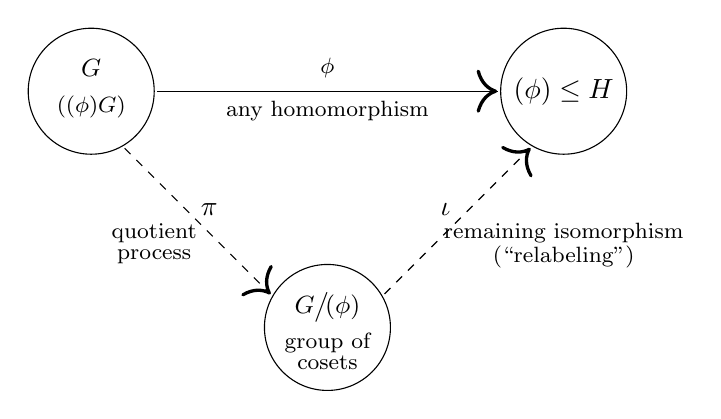
\begin{tikzpicture}[scale=1]
  \tikzset{bigarrow/.style={decoration={markings,mark=at position .99
        with {\arrow[scale=3]{>}}}, postaction={decorate}, 
      shorten >= 1pt, shorten <= 1pt}}
  \tikzstyle{to} = [draw, -stealth]
    \draw (0,0) circle (.8);
    \node at (0,.3) {\small $G$};
    \node at (0,-.2) {\footnotesize ($\Ker(\phi)\normaleq G$)};
    \node at (3,.3) {\footnotesize $\phi$};
    \node at (3,-.25) {\footnotesize any homomorphism};
    %%
    \begin{scope}[shift={(3,-3)}]
      \draw (0,0) circle (.8);
      \node at (0,.25) {\small $G\big/\!\Ker(\phi)$};
      \node at (0,-.2) {\footnotesize group of};
      \node at (0,-.45) {\footnotesize cosets};
    \end{scope}
    %%
    \begin{scope}[shift={(6,0)}]
      \draw (0,0) circle (.8);
      \node at (0,0) {$\Image(\phi)\leq H$};
    \end{scope}
    %%
    \draw [bigarrow] (.8,0) to (5.2,0);
    \draw [bigarrow, dashed] (.4,-.7) to (2.3,-2.6);
    \node at (1.5,-1.5) {$\pi$};
    \node at (.8,-1.8) {\footnotesize quotient};
    \node at (.8,-2.1) {\footnotesize process};
    \draw [bigarrow, dashed] (3.7,-2.6) to (5.6,-.7);
    \node at (4.5,-1.5) {$\iota$};
    \node at (6,-1.8) {\footnotesize remaining isomorphism};
    \node at (6,-2.1) {\footnotesize (``relabeling'')};
  \end{tikzpicture}
  \]
  
\end{frame}

%%====================================================================

\begin{frame}{Visualizing the FHT via Cayley graphs}

  (This is HW 8.14.)

  %%
  %% Commutative diagram of FHT (Cayley graphs)
  %%
  \[
  \begin{tikzpicture}[scale=.9]
   \tikzstyle{every node}=[font=\small]
    \begin{scope}[shift={(0,0)}]
      \draw[cosetBlue, fill=cosetBlue] (45:1) circle (.35);
      \draw[cosetBlue, fill=cosetBlue] (135:1) circle (.35);
      \draw[cosetBlue, fill=cosetBlue] (-45:1) circle (.35);
      \draw[cosetBlue, fill=cosetBlue] (-135:1) circle (.35);
      \draw[cosetBlue, fill=cosetBlue] (45:2) circle (.35);
      \draw[cosetBlue, fill=cosetBlue] (135:2) circle (.35);
      \draw[cosetBlue, fill=cosetBlue] (-45:2) circle (.35);
      \draw[cosetBlue, fill=cosetBlue] (-135:2) circle (.35);
      \draw[cosetBlue, fill=cosetBlue,rotate=45] (1,.35) rectangle (2,-.35);
      \draw[cosetBlue, fill=cosetBlue,rotate=135] (1,.35) rectangle (2,-.35);
      \draw[cosetBlue, fill=cosetBlue,rotate=-45] (1,.35) rectangle (2,-.35);
      \draw[cosetBlue, fill=cosetBlue,rotate=-135] (1,.35) rectangle (2,-.35);
      %%
      \node (1) at (135:2) [v] {$1$};
      \node (i) at (45:2) [v] {$i$};
      \node (k) at (-45:2) [v] {$k$};
      \node (j) at (-135:2) [v] {$j$};
      \node (-1) at (135:1) [v] {$-1$};
      \node (-i) at (45:1) [v] {$-i$};
      \node (-k) at (-45:1) [v] {$-k$};
      \node (-j) at (-135:1) [v] {$-j$};
      \node at (-1.8,.95) {$\mathbf{N}$};
      \node at (-1.8,-.95) {$\mathbf{jN}$};
      \node at (1.8,.95) {$\mathbf{iN}$};
      \node at (1.8,-.95) {$\mathbf{kN}$};
      %%
      \path[b] (1) to (i);
      \path[b] (i) to (-1);
      \path[b] (-1) to (-i);
      \path[b] (-i) to (1);
      %%
      \path[b] (-j) to (-k);
      \path[b] (-k) to (j);
      \path[b] (j) to (k);
      \path[b] (k) to (-j);
      %%
      \path[r] (-k) to (-i);
      \path[r] (-i) to (k);
      \path[r] (k) to (i);
      \path[r] (i) to (-k);
      %% 
      \path[r] (1) to (j);
      \path[r] (j) to (-1);
      \path[r] (-1) to (-j);
      \path[r] (-j) to (1);
      %%
      \path[gg] (1) to (-1);
      \path[gg] (j) to (-j);
      \path[gg] (i) to (-i);
      \path[gg] (k) to (-k);
      %%
      \node at (0,0) {\normalsize $Q_8$};
      \draw[-stealth] (2,0) -- (6.3,0) node[midway,above]{\normalsize $\phi$};
      \draw[-stealth] (0,-2) -- (2,-4) node[midway,below
        left]{\normalsize \quad\small{``\emph{quotient map}''}\quad $\pi$};
    \end{scope}
    %%
    \begin{scope}[shift={(4,-5)}]
    \tikzstyle{every node}=[font=\small]
      \tikzstyle{v} = [circle, draw, fill=lightgray,inner sep=0pt, minimum size=5mm]
      \node at (0,3) {\Large $\phi=\iota\circ\pi$};
      \node (e) at (135:1.5) [v] {$N$};
      \node (h) at (45:1.5) [v] {$iN$};
      \node (v) at (-135:1.5) [v] {$jN$};
      \node (b) at (-45:1.5) [v] {$kN$};
      \draw [bb] (e) to (h);
      \draw [bb] (v) to (b);
      \draw [rr] (e) to (v);
      \draw [rr] (h) to (b);
      \node at (0,0) {\normalsize $Q_8/N$};
      \draw[-stealth] (1.75,1) -- (4,3.5) node[midway,below
        right]{\normalsize $\iota$\quad\small{``\emph{relabeling map}''}};
    \end{scope}
    %%
    \begin{scope}[shift={(8,0)}]
      \tikzstyle{every node}=[font=\small]
      \node (e) at (135:1.5) [v] {$e$};
      \node (h) at (45:1.5) [v] {$v$};
      \node (v) at (-135:1.5) [v] {$h$};
      \node (b) at (-45:1.5) [v] {$r$};
      \draw [bb] (e) to (h);
      \draw [bb] (v) to (b);
      \draw [rr] (e) to (v);
      \draw [rr] (h) to (b);
      \node at (0,0) {\normalsize $V_4$};
    \end{scope}
  \end{tikzpicture}
  \]
  
\end{frame}

%%====================================================================

\begin{frame}{Visualizing the FHT via Cayley tables} 
  
  Here's another way to think about the homomorphism
  \[
  \phi\colon Q_8\longonto V_4,\qquad \phi(i)=v,\;\;\phi(j)=h
  \]
  as the composition of: \smallskip
  \begin{itemize}
  \item a quotient by $N=\Ker(\phi)=\<-1\>=\{\pm1\}$, \smallskip
  \item a \emph{relabeling map} $\iota\colon Q_8/N\to V_4$. 
  \end{itemize}
  
  \vspace{2mm}

  %%
  %% Commutative diagram of FHT: Q_8/<-1>
  %%
  \[
  \begin{tikzpicture}[scale=.42]
  \colorlet{color1}{tLime}
  \colorlet{color-1}{tGreen}
  \colorlet{colori}{tRed}
  \colorlet{color-i}{tPink}
  \colorlet{colorj}{tBlue}
  \colorlet{color-j}{tPurple}
  \colorlet{colork}{tOrange}
  \colorlet{color-k}{tYellow}
  %%  
  \newcommand*{\n}{9}%
    \begin{scope}[shift={(0,0)}]
      \tikzstyle{every node}=[font=\footnotesize]
      %% Left column of colors
      \path[fill=color1] (-.1,8) rectangle ++(1,1);
      \path[fill=color-1] (-.1,7) rectangle ++(1,1);
      \path[fill=colori] (-.1,6) rectangle ++(1,1);
      \path[fill=color-i] (-.1,5) rectangle ++(1,1);
      \path[fill=colorj] (-.1,4) rectangle ++(1,1);
      \path[fill=color-j] (-.1,3) rectangle ++(1,1);
      \path[fill=colork] (-.1,2) rectangle ++(1,1);
      \path[fill=color-k] (-.1,1) rectangle ++(1,1);
      %%
      %% Top row of colors
      \path[fill=color1] (1,9.1) rectangle ++(1,1);
      \path[fill=color-1] (2,9.1) rectangle ++(1,1);
      \path[fill=colori] (3,9.1) rectangle ++(1,1);
      \path[fill=color-i] (4,9.1) rectangle ++(1,1);
      \path[fill=colorj] (5,9.1) rectangle ++(1,1);
      \path[fill=color-j] (6,9.1) rectangle ++(1,1);
      \path[fill=colork] (7,9.1) rectangle ++(1,1);
      \path[fill=color-k] (8,9.1) rectangle ++(1,1);
      %%
      %% All red entries in the table
      \path[fill=color1] (1,8) rectangle ++(1,1);
      \path[fill=color1] (2,7) rectangle ++(1,1);
      \path[fill=color1] (3,5) rectangle ++(1,1);
      \path[fill=color1] (4,6) rectangle ++(1,1);
      \path[fill=color1] (5,3) rectangle ++(1,1);
      \path[fill=color1] (6,4) rectangle ++(1,1);
      \path[fill=color1] (7,1) rectangle ++(1,1);
      \path[fill=color1] (8,2) rectangle ++(1,1);
      %%
      \path[fill=color-1] (1,7) rectangle ++(1,1);
      \path[fill=color-1] (2,8) rectangle ++(1,1);
      \path[fill=color-1] (3,6) rectangle ++(1,1);
      \path[fill=color-1] (4,5) rectangle ++(1,1);
      \path[fill=color-1] (5,4) rectangle ++(1,1);
      \path[fill=color-1] (6,3) rectangle ++(1,1);
      \path[fill=color-1] (7,2) rectangle ++(1,1);
      \path[fill=color-1] (8,1) rectangle ++(1,1);
      %%
      \path[fill=colori] (1,6) rectangle ++(1,1);
      \path[fill=colori] (2,5) rectangle ++(1,1);
      \path[fill=colori] (3,8) rectangle ++(1,1);
      \path[fill=colori] (4,7) rectangle ++(1,1);
      \path[fill=colori] (5,1) rectangle ++(1,1);
      \path[fill=colori] (6,2) rectangle ++(1,1);
      \path[fill=colori] (7,4) rectangle ++(1,1);
      \path[fill=colori] (8,3) rectangle ++(1,1);
      %%
      \path[fill=color-i] (1,5) rectangle ++(1,1);
      \path[fill=color-i] (2,6) rectangle ++(1,1);
      \path[fill=color-i] (3,7) rectangle ++(1,1);
      \path[fill=color-i] (4,8) rectangle ++(1,1);
      \path[fill=color-i] (5,2) rectangle ++(1,1);
      \path[fill=color-i] (6,1) rectangle ++(1,1);
      \path[fill=color-i] (7,3) rectangle ++(1,1);
      \path[fill=color-i] (8,4) rectangle ++(1,1);
      %%
      \path[fill=colorj] (1,4) rectangle ++(1,1);
      \path[fill=colorj] (2,3) rectangle ++(1,1);
      \path[fill=colorj] (3,2) rectangle ++(1,1);
      \path[fill=colorj] (4,1) rectangle ++(1,1);
      \path[fill=colorj] (5,8) rectangle ++(1,1);
      \path[fill=colorj] (6,7) rectangle ++(1,1);
      \path[fill=colorj] (7,5) rectangle ++(1,1);
      \path[fill=colorj] (8,6) rectangle ++(1,1);
      %%
      \path[fill=color-j] (1,3) rectangle ++(1,1);
      \path[fill=color-j] (2,4) rectangle ++(1,1);
      \path[fill=color-j] (3,1) rectangle ++(1,1);
      \path[fill=color-j] (4,2) rectangle ++(1,1);
      \path[fill=color-j] (5,7) rectangle ++(1,1);
      \path[fill=color-j] (6,8) rectangle ++(1,1);
      \path[fill=color-j] (7,6) rectangle ++(1,1);
      \path[fill=color-j] (8,5) rectangle ++(1,1);
      %%
      \path[fill=colork] (1,2) rectangle ++(1,1);
      \path[fill=colork] (2,1) rectangle ++(1,1);
      \path[fill=colork] (3,3) rectangle ++(1,1);
      \path[fill=colork] (4,4) rectangle ++(1,1);
      \path[fill=colork] (5,6) rectangle ++(1,1);
      \path[fill=colork] (6,5) rectangle ++(1,1);
      \path[fill=colork] (7,8) rectangle ++(1,1);
      \path[fill=colork] (8,7) rectangle ++(1,1);
      %%
      \path[fill=color-k] (1,1) rectangle ++(1,1);
      \path[fill=color-k] (2,2) rectangle ++(1,1);
      \path[fill=color-k] (3,4) rectangle ++(1,1);
      \path[fill=color-k] (4,3) rectangle ++(1,1);
      \path[fill=color-k] (5,5) rectangle ++(1,1);
      \path[fill=color-k] (6,6) rectangle ++(1,1);
      \path[fill=color-k] (7,7) rectangle ++(1,1);
      \path[fill=color-k] (8,8) rectangle ++(1,1);
      %%
      \foreach \i in {1,...,\n} {
        \draw [very thin] (\i,1) -- (\i,\n); 
        \draw [very thin] (\i,\n+.1) -- (\i,\n+1.1); 
        \draw [very thin] (1,\i) -- (\n,\i); 
        \draw [very thin] (-.1,\i) -- (.9,\i); 
      } 
      \draw (-.1,1) rectangle ++(1,8);
      \draw (1,9.1) rectangle ++(8,1);
      \node at (0.4,8.5) {$1$};
      \node at (0.4,7.5) {$-1$};
      \node at (0.4,6.5) {$i$};
      \node at (0.4,5.5) {$-i$}; 
      \node at (0.4,4.5) {$j$}; 
      \node at (0.4,3.5) {$-j$};
      \node at (0.4,2.5) {$k$};
      \node at (0.4,1.5) {$-k$};
      %% 
      \node at (1.5,9.6) {$1$};
      \node at (2.5,9.6) {$-1$};
      \node at (3.5,9.6) {$i$};
      \node at (4.5,9.6) {$-i$}; 
      \node at (5.5,9.6) {$j$}; 
      \node at (6.5,9.6) {$-j$};
      \node at (7.5,9.6) {$k$};
      \node at (8.5,9.6) {$-k$};
      %%
      \node at (1.5,8.5) {$1$};
      \node at (1.5,7.5) {$-1$};
      \node at (1.5,6.5) {$i$};
      \node at (1.5,5.5) {$-i$}; 
      \node at (1.5,4.5) {$j$}; 
      \node at (1.5,3.5) {$-j$};
      \node at (1.5,2.5) {$k$};
      \node at (1.5,1.5) {$-k$};
      %%
      \node at (2.5,8.5) {$-1$};
      \node at (2.5,7.5) {$1$};
      \node at (2.5,6.5) {$-i$};
      \node at (2.5,5.5) {$i$}; 
      \node at (2.5,4.5) {$-j$}; 
      \node at (2.5,3.5) {$j$};
      \node at (2.5,2.5) {$-k$};
      \node at (2.5,1.5) {$k$};
      %%
      \node at (3.5,8.5) {$i$};
      \node at (3.5,7.5) {$-i$};
      \node at (3.5,6.5) {$-1$};
      \node at (3.5,5.5) {$1$}; 
      \node at (3.5,4.5) {$-k$}; 
      \node at (3.5,3.5) {$k$};
      \node at (3.5,2.5) {$j$};
      \node at (3.5,1.5) {$-j$};
      %%
      \node at (4.5,8.5) {$-i$};
      \node at (4.5,7.5) {$i$};
      \node at (4.5,6.5) {$1$};
      \node at (4.5,5.5) {$-1$}; 
      \node at (4.5,4.5) {$k$}; 
      \node at (4.5,3.5) {$-k$};
      \node at (4.5,2.5) {$-j$};
      \node at (4.5,1.5) {$j$};
      %%
      \node at (5.5,8.5) {$j$};
      \node at (5.5,7.5) {$-j$};
      \node at (5.5,6.5) {$k$};
      \node at (5.5,5.5) {$-k$}; 
      \node at (5.5,4.5) {$-1$}; 
      \node at (5.5,3.5) {$1$};
      \node at (5.5,2.5) {$-i$};
      \node at (5.5,1.5) {$i$};
      %%
      \node at (6.5,8.5) {$-j$};
      \node at (6.5,7.5) {$j$};
      \node at (6.5,6.5) {$-k$};
      \node at (6.5,5.5) {$k$}; 
      \node at (6.5,4.5) {$1$}; 
      \node at (6.5,3.5) {$-1$};
      \node at (6.5,2.5) {$i$};
      \node at (6.5,1.5) {$-i$};
      %%
      \node at (7.5,8.5) {$k$};
      \node at (7.5,7.5) {$-k$};
      \node at (7.5,6.5) {$-j$};
      \node at (7.5,5.5) {$j$}; 
      \node at (7.5,4.5) {$i$}; 
      \node at (7.5,3.5) {$-i$};
      \node at (7.5,2.5) {$-1$};
      \node at (7.5,1.5) {$1$};
      %%
      \node at (8.5,8.5) {$-k$};
      \node at (8.5,7.5) {$k$};
      \node at (8.5,6.5) {$j$};
      \node at (8.5,5.5) {$-j$}; 
      \node at (8.5,4.5) {$-i$}; 
      \node at (8.5,3.5) {$i$};
      \node at (8.5,2.5) {$1$};
      \node at (8.5,1.5) {$-1$};
      %%
      \filldraw[fill=white,opacity=0.7] 
      (1,1)--(9,1)--(9,9)--(1,9)--cycle;
      \draw[thick] (3,1)--(3,9);
      \draw[thick] (5,1)--(5,9);
      \draw[thick] (7,1)--(7,9); 
      \draw[thick] (1,3)--(9,3);
      \draw[thick] (1,5)--(9,5);
      \draw[thick] (1,7)--(9,7);
      \node at (2,8) {\large\bf $\mathbf{N}$};
      \node at (4,8) {\large\bf $\mathbf{iN}$};
      \node at (6,8) {\large\bf $\mathbf{jN}$};
      \node at (8,8) {\large\bf $\mathbf{kN}$};
      \node at (2,6) {\large\bf $\mathbf{iN}$};
      \node at (4,6) {\large\bf $\mathbf{N}$};
      \node at (6,6) {\large\bf $\mathbf{kN}$};
      \node at (8,6) {\large\bf $\mathbf{jN}$};
      \node at (2,4) {\large\bf $\mathbf{jN}$};
      \node at (4,4) {\large\bf $\mathbf{kN}$};
      \node at (6,4) {\large\bf $\mathbf{N}$};
      \node at (8,4) {\large\bf $\mathbf{iN}$};
      \node at (2,2) {\large\bf $\mathbf{kN}$};
      \node at (4,2) {\large\bf $\mathbf{jN}$};
      \node at (6,2) {\large\bf $\mathbf{iN}$};
      \node at (8,2) {\large\bf $\mathbf{N}$};
      \draw[-stealth] (10,5) -- (13,5) node[midway,above]{\large $\iota$};
    \end{scope}
    %%
    \begin{scope}[shift={(14,0)}]
      \tikzstyle{every node}=[font=\footnotesize]
      %% Left column of colors
      \path[fill=color1] (-.1,8) rectangle ++(1,1);
      \path[fill=color-1] (-.1,7) rectangle ++(1,1);
      \path[fill=colori] (-.1,6) rectangle ++(1,1);
      \path[fill=color-i] (-.1,5) rectangle ++(1,1);
      \path[fill=colorj] (-.1,4) rectangle ++(1,1);
      \path[fill=color-j] (-.1,3) rectangle ++(1,1);
      \path[fill=colork] (-.1,2) rectangle ++(1,1);
      \path[fill=color-k] (-.1,1) rectangle ++(1,1);
      %%
      %% Top row of colors
      \path[fill=color1] (1,9.1) rectangle ++(1,1);
      \path[fill=color-1] (2,9.1) rectangle ++(1,1);
      \path[fill=colori] (3,9.1) rectangle ++(1,1);
      \path[fill=color-i] (4,9.1) rectangle ++(1,1);
      \path[fill=colorj] (5,9.1) rectangle ++(1,1);
      \path[fill=color-j] (6,9.1) rectangle ++(1,1);
      \path[fill=colork] (7,9.1) rectangle ++(1,1);
      \path[fill=color-k] (8,9.1) rectangle ++(1,1);
      %
      %% All red entries in the table
      \path[fill=color1] (1,8) rectangle ++(1,1);
      \path[fill=color1] (2,7) rectangle ++(1,1);
      \path[fill=color1] (3,5) rectangle ++(1,1);
      \path[fill=color1] (4,6) rectangle ++(1,1);
      \path[fill=color1] (5,3) rectangle ++(1,1);
      \path[fill=color1] (6,4) rectangle ++(1,1);
      \path[fill=color1] (7,1) rectangle ++(1,1);
      \path[fill=color1] (8,2) rectangle ++(1,1);
      %%
      \path[fill=color-1] (1,7) rectangle ++(1,1);
      \path[fill=color-1] (2,8) rectangle ++(1,1);
      \path[fill=color-1] (3,6) rectangle ++(1,1);
      \path[fill=color-1] (4,5) rectangle ++(1,1);
      \path[fill=color-1] (5,4) rectangle ++(1,1);
      \path[fill=color-1] (6,3) rectangle ++(1,1);
      \path[fill=color-1] (7,2) rectangle ++(1,1);
      \path[fill=color-1] (8,1) rectangle ++(1,1);
      %%
      \path[fill=colori] (1,6) rectangle ++(1,1);
      \path[fill=colori] (2,5) rectangle ++(1,1);
      \path[fill=colori] (3,8) rectangle ++(1,1);
      \path[fill=colori] (4,7) rectangle ++(1,1);
      \path[fill=colori] (5,1) rectangle ++(1,1);
      \path[fill=colori] (6,2) rectangle ++(1,1);
      \path[fill=colori] (7,4) rectangle ++(1,1);
      \path[fill=colori] (8,3) rectangle ++(1,1);
      %%
      \path[fill=color-i] (1,5) rectangle ++(1,1);
      \path[fill=color-i] (2,6) rectangle ++(1,1);
      \path[fill=color-i] (3,7) rectangle ++(1,1);
      \path[fill=color-i] (4,8) rectangle ++(1,1);
      \path[fill=color-i] (5,2) rectangle ++(1,1);
      \path[fill=color-i] (6,1) rectangle ++(1,1);
      \path[fill=color-i] (7,3) rectangle ++(1,1);
      \path[fill=color-i] (8,4) rectangle ++(1,1);
      %%
      \path[fill=colorj] (1,4) rectangle ++(1,1);
      \path[fill=colorj] (2,3) rectangle ++(1,1);
      \path[fill=colorj] (3,2) rectangle ++(1,1);
      \path[fill=colorj] (4,1) rectangle ++(1,1);
      \path[fill=colorj] (5,8) rectangle ++(1,1);
      \path[fill=colorj] (6,7) rectangle ++(1,1);
      \path[fill=colorj] (7,5) rectangle ++(1,1);
      \path[fill=colorj] (8,6) rectangle ++(1,1);
      %%
      \path[fill=color-j] (1,3) rectangle ++(1,1);
      \path[fill=color-j] (2,4) rectangle ++(1,1);
      \path[fill=color-j] (3,1) rectangle ++(1,1);
      \path[fill=color-j] (4,2) rectangle ++(1,1);
      \path[fill=color-j] (5,7) rectangle ++(1,1);
      \path[fill=color-j] (6,8) rectangle ++(1,1);
      \path[fill=color-j] (7,6) rectangle ++(1,1);
      \path[fill=color-j] (8,5) rectangle ++(1,1);
      %%
      \path[fill=colork] (1,2) rectangle ++(1,1);
      \path[fill=colork] (2,1) rectangle ++(1,1);
      \path[fill=colork] (3,3) rectangle ++(1,1);
      \path[fill=colork] (4,4) rectangle ++(1,1);
      \path[fill=colork] (5,6) rectangle ++(1,1);
      \path[fill=colork] (6,5) rectangle ++(1,1);
      \path[fill=colork] (7,8) rectangle ++(1,1);
      \path[fill=colork] (8,7) rectangle ++(1,1);
      %%
      \path[fill=color-k] (1,1) rectangle ++(1,1);
      \path[fill=color-k] (2,2) rectangle ++(1,1);
      \path[fill=color-k] (3,4) rectangle ++(1,1);
      \path[fill=color-k] (4,3) rectangle ++(1,1);
      \path[fill=color-k] (5,5) rectangle ++(1,1);
      \path[fill=color-k] (6,6) rectangle ++(1,1);
      \path[fill=color-k] (7,7) rectangle ++(1,1);
      \path[fill=color-k] (8,8) rectangle ++(1,1);
      %%
      \foreach \i in {1,...,\n} {
        \draw [very thin] (\i,1) -- (\i,\n); 
        \draw [very thin] (\i,\n+.1) -- (\i,\n+1.1); 
        \draw [very thin] (1,\i) -- (\n,\i); 
        \draw [very thin] (-.1,\i) -- (.9,\i); 
      } 
      \draw (-.1,1) rectangle ++(1,8);
      \draw (1,9.1) rectangle ++(8,1);
      \node at (0.4,8.5) {$1$};
      \node at (0.4,7.5) {$-1$};
      \node at (0.4,6.5) {$i$};
      \node at (0.4,5.5) {$-i$}; 
      \node at (0.4,4.5) {$j$}; 
      \node at (0.4,3.5) {$-j$};
      \node at (0.4,2.5) {$k$};
      \node at (0.4,1.5) {$-k$};
      %% 
      \node at (1.5,9.6) {$1$};
      \node at (2.5,9.6) {$-1$};
      \node at (3.5,9.6) {$i$};
      \node at (4.5,9.6) {$-i$}; 
      \node at (5.5,9.6) {$j$}; 
      \node at (6.5,9.6) {$-j$};
      \node at (7.5,9.6) {$k$};
      \node at (8.5,9.6) {$-k$};
      %%
      \node at (1.5,8.5) {$1$};
      \node at (1.5,7.5) {$-1$};
      \node at (1.5,6.5) {$i$};
      \node at (1.5,5.5) {$-i$}; 
      \node at (1.5,4.5) {$j$}; 
      \node at (1.5,3.5) {$-j$};
      \node at (1.5,2.5) {$k$};
      \node at (1.5,1.5) {$-k$};
      %%
      \node at (2.5,8.5) {$-1$};
      \node at (2.5,7.5) {$1$};
      \node at (2.5,6.5) {$-i$};
      \node at (2.5,5.5) {$i$}; 
      \node at (2.5,4.5) {$-j$}; 
      \node at (2.5,3.5) {$j$};
      \node at (2.5,2.5) {$-k$};
      \node at (2.5,1.5) {$k$};
      %%
      \node at (3.5,8.5) {$i$};
      \node at (3.5,7.5) {$-i$};
      \node at (3.5,6.5) {$-1$};
      \node at (3.5,5.5) {$1$}; 
      \node at (3.5,4.5) {$-k$}; 
      \node at (3.5,3.5) {$k$};
      \node at (3.5,2.5) {$j$};
      \node at (3.5,1.5) {$-j$};
      %%
      \node at (4.5,8.5) {$-i$};
      \node at (4.5,7.5) {$i$};
      \node at (4.5,6.5) {$1$};
      \node at (4.5,5.5) {$-1$}; 
      \node at (4.5,4.5) {$k$}; 
      \node at (4.5,3.5) {$-k$};
      \node at (4.5,2.5) {$-j$};
      \node at (4.5,1.5) {$j$};
      %%
      \node at (5.5,8.5) {$j$};
      \node at (5.5,7.5) {$-j$};
      \node at (5.5,6.5) {$k$};
      \node at (5.5,5.5) {$-k$}; 
      \node at (5.5,4.5) {$-1$}; 
      \node at (5.5,3.5) {$1$};
      \node at (5.5,2.5) {$-i$};
      \node at (5.5,1.5) {$i$};
      %%
      \node at (6.5,8.5) {$-j$};
      \node at (6.5,7.5) {$j$};
      \node at (6.5,6.5) {$-k$};
      \node at (6.5,5.5) {$k$}; 
      \node at (6.5,4.5) {$1$}; 
      \node at (6.5,3.5) {$-1$};
      \node at (6.5,2.5) {$i$};
      \node at (6.5,1.5) {$-i$};
      %%
      \node at (7.5,8.5) {$k$};
      \node at (7.5,7.5) {$-k$};
      \node at (7.5,6.5) {$-j$};
      \node at (7.5,5.5) {$j$}; 
      \node at (7.5,4.5) {$i$}; 
      \node at (7.5,3.5) {$-i$};
      \node at (7.5,2.5) {$-1$};
      \node at (7.5,1.5) {$1$};
      %%
      \node at (8.5,8.5) {$-k$};
      \node at (8.5,7.5) {$k$};
      \node at (8.5,6.5) {$j$};
      \node at (8.5,5.5) {$-j$}; 
      \node at (8.5,4.5) {$-i$}; 
      \node at (8.5,3.5) {$i$};
      \node at (8.5,2.5) {$1$};
      \node at (8.5,1.5) {$-1$};
      %%
      \filldraw[fill=white,opacity=0.7] 
      (1,1)--(9,1)--(9,9)--(1,9)--cycle;
      \draw[thick] (3,1)--(3,9);
      \draw[thick] (5,1)--(5,9);
      \draw[thick] (7,1)--(7,9); 
      \draw[thick] (1,3)--(9,3);
      \draw[thick] (1,5)--(9,5);
      \draw[thick] (1,7)--(9,7);
      \node at (2,8) {\large\bf $\mathbf{e}$};
      \node at (4,8) {\large\bf $\mathbf{v}$};
      \node at (6,8) {\large\bf $\mathbf{h}$};
      \node at (8,8) {\large\bf $\mathbf{r}$};
      \node at (2,6) {\large\bf $\mathbf{v}$};
      \node at (4,6) {\large\bf $\mathbf{e}$};
      \node at (6,6) {\large\bf $\mathbf{r}$};
      \node at (8,6) {\large\bf $\mathbf{h}$};
      \node at (2,4) {\large\bf $\mathbf{h}$};
      \node at (4,4) {\large\bf $\mathbf{r}$};
      \node at (6,4) {\large\bf $\mathbf{e}$};
      \node at (8,4) {\large\bf $\mathbf{v}$};
      \node at (2,2) {\large\bf $\mathbf{r}$};
      \node at (4,2) {\large\bf $\mathbf{h}$};
      \node at (6,2) {\large\bf $\mathbf{v}$};
      \node at (8,2) {\large\bf $\mathbf{e}$};
    \end{scope}
  \end{tikzpicture}
  \]
  
\end{frame}

%%====================================================================

\begin{frame}{FHT preliminaries}
  
  \begin{block}{Proposition (HW 8.9)}
    The \Balert{kernel} of any homomorphism $\phi\colon G\to
    H$, is a \Balert{normal subgroup}.
  \end{block}
  
  \begin{exampleblock}{Proof} \Pause
    Let $N:=\Ker(\phi)$. First, we'll show that it's a
    subgroup. \Pause \Balert{Take any $a,b\in N$}. \medskip\pause
    
    \textbf{Identity}: $\phi(e)=e$. $\hfill\checkmark$
    
    \medskip\pause
    
    \textbf{Closure}:
    $\phi(ab)\Pause=\phi(a)\,\phi(b)\Pause=e\cdot e=e$. $\hfill\checkmark$
    
    \medskip\pause
    
    \textbf{Inverse}:
    $\phi(a^{-1})\Pause=\phi(a)^{-1}\Pause=e^{-1}\Pause=e$. 
    $\hfill\checkmark$ \medskip\pause
    
    Now we'll show it's normal. \Pause Take any $n\in N$. We'll show that
    $gng^{-1}\in N$ for all $g\in G$. \medskip\pause
    
    By the homomorphism property,
    \[
    \phi(gng^{-1})\Pause=\phi(g)\,\phi(n)\,\phi(g^{-1})
    \Pause=\phi(g)\cdot e\cdot\phi(g)^{-1}\Pause=e.
    \]
    \Pause Therefore, $gng^{-1}\in\Ker(\phi)$. $\hfill\Box$
  \end{exampleblock}
  
  \Pause
  
  \begin{alertblock}{Key observation}
    Given any homomorphism $\phi\colon G\to H$, we can \emph{always}
    form the quotient group $G/\Ker(\phi)$.
  \end{alertblock}
  
\end{frame}

%%====================================================================

\begin{frame}{FHT preliminaries}
  
  \begin{block}{Proposition (HW 8.10)}
    Let $\phi\colon G\to H$ be a homomorphism. Then each
    \Balert{preimage} $\phi^{-1}(h)$ is a \Balert{coset} of
    $\Ker(\phi)$.
  \end{block}
  
  \begin{exampleblock}{Proof} \Pause
    Let $N=\Ker(\phi)$ and take any $g\in\phi^{-1}(h)$. (This means
    \Balert{$\phi(g)=h$}.) \medskip\Pause
    
    We claim that \Alert{$\phi^{-1}(h)=gN$}. \Pause We need to verify both
    $\subseteq$ and $\supseteq$. \medskip\pause
    
    ``$\subseteq$'': Take $a\in\phi^{-1}(h)$, i.e.,
    \Balert{$\phi(a)=h$}. \Pause We need to show that 
    $a\in gN$. \medskip\pause
    
    From basic properties of cosets, we have the equivalences
    \[
    a\in gN\Pause\quad\Longleftrightarrow\quad 
    aN=gN\Pause\quad\Longleftrightarrow\quad 
    g^{-1}aN=N \Pause\quad\Longleftrightarrow\quad 
    g^{-1}a\in N.
    \]
    \Pause This last condition is true because
    \[
    \phi(g^{-1}a)\Pause=\phi(g)^{-1}\phi(a)\Pause
    =h^{-1}\cdot h=1_H. \tag*{$\checkmark$}
    \]
    \pause
    
    ``$\supseteq$'': Pick any $gn\in gN$. \Pause This is in
    $\phi^{-1}(h)$ because
    \[
    \phi(gn)\Pause=\phi(g)\phi(n)\Pause=h\cdot 1_H\Pause=h. \tag*{$\checkmark$}
    \]
    \vspace{-3mm}
  \end{exampleblock}
    
\end{frame}

%%====================================================================

\begin{frame}{Proof of the FHT}
  
  \begin{block}{Fundamental homomorphism theorem} 
    If $\phi\colon G\to H$ is a homomorphism, then $\Image(\phi)\cong
    G/\Ker(\phi)$.
  \end{block}
  
  \begin{exampleblock}{Proof} \Pause
    We'll construct an explicit map $\iota\colon
    G/\Ker(\phi)\longrightarrow\Image(\phi)$ and prove that it's an
    isomorphism.
    
    \medskip\pause
    
    Let $N=\Ker(\phi)$, and recall that $G/N=\{gN\mid g\in
    G\}$. \Pause Define
    \[
    \Alert{\iota\colon G/N\longrightarrow\Image(\phi)\,,\qquad\quad \iota\colon
      gN\longmapsto\Pause\phi(g)}\,.
    \]
    
    \Pause
    
    \pause $\bullet$ \underline{\emph{Show $\iota$ is well-defined}}\,: \Pause
    We must show that if $aN=bN$, then $\iota(aN)=\iota(bN)$.
    
    \medskip\Pause 
    
    Suppose $aN=bN$. \Pause We have
    \[
    aN=bN \quad\Longrightarrow\quad\Pause b^{-1}aN=N
    \quad\Longrightarrow\quad\Pause b^{-1}a\in N\,.\Pause
    \]
    \pause By definition of $b^{-1}a\in\Ker(\phi)$,%\Pause
    \[
    1_H=\phi(b^{-1}a)\Pause=\phi(b^{-1})\,\phi(a)\Pause
    =\phi(b)^{-1}\,\phi(a)\Pause\quad\Longrightarrow\quad
    {\color{blue}\phi(a)=\phi(b)}\,.
    \]
    
    \Pause
    %\vspace{-0.15in}
    
    By definition of $\iota$:\quad
    $\iota(aN)={\color{blue}\phi(a)}\Pause={\color{blue}\phi(b)}\Pause
    =\iota(bN)$. $\hfill\checkmark$
  \end{exampleblock}

\end{frame}

%%====================================================================

\begin{frame}{Proof of FHT (cont.) [{\small Recall: 
    $\quad \iota\colon G/N\rightarrow\Image(\phi)\,,\quad\iota\colon 
    gN\mapsto\phi(g)$}]} 

  \begin{exampleblock}{Proof (cont.)}
    $\bullet$ \underline{\emph{Show $\iota$ is a homomorphism}}\,: \Pause We must
    show that $\iota(aN\cdot bN)=\iota(aN)\,\iota(bN)$. 
    
    \medskip\Pause
    
    \begin{center}\renewcommand{\arraystretch}{1.2}
      \begin{tabular}{rcllll}
        $\iota(aN\cdot bN)$ & $=$ & $\iota(abN)$ &&&($aN\cdot bN:=abN$)\Pause
        \\  
        & $=$ & $\phi(ab)$ &&& (definition of $\iota$) \Pause \\
        & $=$ & $\phi(a)\,\phi(b)$&&& ($\phi$ is a homomorphism)\Pause\\
        & $=$ & $\iota(aN)\,\iota(bN$) &&& (definition of $\iota$)
      \end{tabular}
    \end{center}
    
    \Pause Thus, $\iota$ is a homomorphism. $\hfill\checkmark$ 
    
    \bigskip\Pause
    
    \pause $\bullet$ \underline{\emph{Show $\iota$ is surjective (onto)}}\,:
    
    \medskip\Pause
    
    Take any element in the codomain (here, $\Image(\phi)$). \Pause We need to
    find an element in the domain (here, $G/N$) that gets mapped to it
    by $\iota$.
    
    \Pause\bigskip
    
    Pick any $\phi(a)\in\Image(\phi)$. \Pause By defintion, $\iota(aN)=\phi(a)$,
    hence $\iota$ is surjective. $\hfill\checkmark$ 
    
  \end{exampleblock}
  
\end{frame}

%%====================================================================

\begin{frame}{Proof of FHT (cont.) [{\small Recall: 
        $\quad\iota\colon G/N\rightarrow\Image(\phi)\,,\quad\iota\colon 
        gN\mapsto\phi(g)$}]}
  
  \begin{exampleblock}{Proof (cont.)} %\Pause
    
    $\bullet$ \underline{\emph{Show $\iota$ is injective (1--1)}}\,: \Pause
    We must show that $\iota(aN)=\iota(bN)$ implies $aN=bN$.
    
    \pause
    \bigskip
    
    Suppose that $\iota(aN)=\iota(bN)$. \Pause Then
    
    \begin{center}\renewcommand{\arraystretch}{1.2}
      \begin{tabular}{rclll}
        $\iota(aN)=\iota(bN)$ & $\Longrightarrow$ & $\phi(a)=\phi(b)$ & 
        (by definition) \Pause \\
        & $\Longrightarrow$ & $\phi(b)^{-1}\,\phi(a)=1_H$ \Pause & \\ 
        & $\Longrightarrow$ & $\phi(b^{-1}a)=1_H$ &
        ($\phi$ is a homom.) \Pause \\
        & $\Longrightarrow$ & $b^{-1}a\in N$ &
        (definition of $\Ker(\phi)$) \Pause \\
        & $\Longrightarrow$ & $b^{-1}aN=N$ & 
        ($aH=H\;\Leftrightarrow\;a\in H$) \Pause \\
        & $\Longrightarrow$ & $aN=bN$ & 
      \end{tabular}
    \end{center}
    
    Thus, $\iota$ is injective. $\hfill\checkmark$ 
    
    \bigskip\pause
    
    In summary, since $\iota\colon G/N\to\Image(\phi)$ is a well-defined
    homomorphism that is \Alert{injective} (1--1) and
    {\color{blue}surjective} (onto), it is an \textbf{isomorphism}.
    
    \bigskip\Pause
    
    Therefore, $G/N\cong\Image(\phi)$, and the FHT is proven. $\hfill\Box$
    
  \end{exampleblock}
  
\end{frame}

%%====================================================================

\begin{frame}{Consequences of the FHT} 
  
  \begin{block}{Corollary}
    If $\phi\colon G\to H$ is a homomorphism, then $\Image\phi\leq H$.
  \end{block}

  \Pause
    
  \begin{exampleblock}{The two ``extreme cases''}%\Pause
    \begin{itemize}
    \item If $\phi\colon G\into H$ is an \Balert{embedding}, then
      $\Ker(\phi)=\{1_G\}$. \Pause The FHT says that
      \[
      \Image(\phi)\cong G/\{1_G\}\cong G.
      \]    
      \vspace{-4mm}\Pause
    \item If $\phi\colon G\to H$ is the \Balert{trivial map}
      $\phi(g)=1_H$ for all $h\in G$, then $\Ker(\phi)=G$. \Pause The FHT
      says that
      \[
      \{1_H\}=\Image(\phi)\cong G/G.
      \]
      \vspace{-3mm}
    \end{itemize}  
  \end{exampleblock}
  
  \smallskip\Pause
  
  Let's use the FHT to determine all homomorphisms $\phi\colon
  C_4\to C_3$.
  
  \smallskip\Pause
  
  \begin{itemize}
  \item By the FHT, $G/\Ker\phi\cong\Image\phi\leq C_3$, and so \Pause
    $|\Image\phi|=1$ or $3$. \smallskip\Pause
  \item Since $\Ker\phi\leq C_4$, Lagrange's Theorem also tells us that
    $|\Ker\phi|\in\{1,2,4\}$, \Pause and hence
    $|\Image\phi|=|G/\Ker\phi|\in\{1,2,4\}$. \medskip\Pause
  \end{itemize}
  
  Thus, $|\Image\phi|=1$, and so the \emph{only} homomorphism $\phi\colon C_4\to
  C_3$ is the trivial one.
\end{frame}

%%====================================================================

\begin{frame}{Consequences of the FHT} %\Pause
  
  Let's do a more complicated example: find all homomorphisms
  $\phi\colon\Z_{44}\to\Z_{16}$. \medskip\Pause
  
  By the FHT,
  \[
  \Z_{44}/\Ker(\phi)\cong\Image(\phi)\leq\Z_{16}.
  \]
  \Pause This means that $44/|\Ker(\phi)|$ must be $1$, $2$, $4$, \st{$8$},
  or \st{$16$}.
  
  \medskip\Pause
  
  Also, $|\Ker(\phi)|$ must divide $44$. \Pause We are left with
  three cases: \Balert{$|\Ker(\phi)|=44$, $22$, or
    $11$}. \smallskip\Pause
  
  \begin{exampleblock}{Reminder}
    For each $d\mid n$, the group $\Z_n$ has a unique
    subgroup of order $d$, which is $\<n/d\>$. 
  \end{exampleblock}
  
  \smallskip\Pause
  
  \begin{itemize}
  \item \textbf{Case 1}: \Balert{$|\Ker(\phi)|=44$}, which forces
    $|\Image(\phi)|=1$, and so $\phi(1)=0$ is the trivial
    homomorphism. \medskip\Pause
  \item \textbf{Case 2}: \Balert{$|\Ker(\phi)|=22$}. \Pause By the FHT,
    $|\Image(\phi)|=2$, which means $\Image(\phi)=\{0,8\}$, and so
    $\phi(1)=8$. \medskip\Pause
  \item \textbf{Case 3}: \Balert{$|\Ker(\phi)|=11$}. \Pause By the FHT,
    $|\Image(\phi)|=4$, which means $\Image(\phi)=\{0,4,8,12\}$. \medskip\Pause
    
    There are two subcases: $\phi(1)=4$ or $\phi(1)=12$.
  \end{itemize}
  
\end{frame}

%%====================================================================

\begin{frame}{What does ``well-defined'' really mean?} 
  
  Recall that we've seen the term ``\textbf{well-defined}'' arise in
  different contexts: \smallskip\Pause
  \begin{itemize}
  \item a well-defined \Balert{binary operation} on a set $G/N$
    of cosets, \smallskip\Pause
  \item a well-defined \Alert{function} $\iota\colon G/N\to H$ from a
    set (group) of cosets. \Pause
  \end{itemize}
  
  \medskip
  
  In both of these cases, well-defined means that: 
  \begin{center}
    ``\emph{our definition doesn't depend on our choice of coset representative}.'' 
  \end{center}
  
  \Pause
  
  Formally:
  
  \begin{itemize}
  \item If $N\normaleq G$, then $aN\cdot bN:=abN$ is a
    {\color{blue}well-defined binary operation} on the set $G/N$ of
    cosets, \Pause because
    \[
    \text{if\; $a_1N=a_2N$\; and\; $b_1N=b_2N$},\;\;\Pause \text{then\; $a_1b_1N=a_2b_2N$}. 
    \] \vspace{-5mm}\Pause
  \item The map $\iota\colon G/N\to H$, where $\iota(aN)=\phi(a)$, is a 
    {\color{red}well-defined homomorphism}, \Pause meaning that    
    \[
    \text{if\; $aN=bN$,\; then\, $\iota(aN)=\iota(bN)$\, (that is, $\phi(a)=\phi(b)$) holds.}
    \]
  \end{itemize}
  
  \vspace{-1mm}\Pause
  
  \begin{alertblock}{Remark}
    Whenever we define a map and the domain is a \emph{quotient}, we
    must show it's well-defined.
  \end{alertblock}
  
\end{frame}

%%====================================================================

\begin{frame}{What does ``well-defined'' really mean?}

  In some sense, well-defined and injective are ``dual'' concepts: \smallskip
  \begin{itemize}
  \item $f$ is \Balert{well-defined} if the same input cannot map to
    different outputs
  \item (that is, $f$ is a function!)
  \item $f$ is \Balert{injective} if different inputs cannot map to
    the same output.
  \end{itemize}
  
  
  %% Picture of 1-1 vs. well-defined
  %%
  \[
  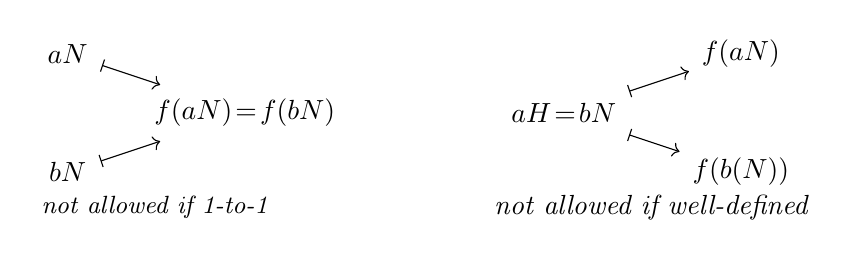
\begin{tikzpicture}[scale=.6,xscale=1.5]
    \begin{scope}[scale=2.5,inner sep=5pt]
      \node at (.5,-.8) {\small \emph{not allowed if 1-to-1}};
      \node (a) at (0,.5) {$aN$};
      \node (f) at (1,0) {$f(aN)\!=\!f(bN)$};
      \node (b) at (0,-.5) {$bN$};
      \draw[|->] (a) to (f);
      \draw[|->] (b) to (f);
    \end{scope}
    %%
    \begin{scope}[shift={(7,0)},scale=2.5,inner sep=4.5pt]
      \node at (.5,-.8) {\emph{not allowed if well-defined}};
      \node (fA) at (1,.5) {$f(aN)$};
      \node (aH) at (0,0) {$aH\!=\!bN$};
      \node (fB) at (1,-.5) {$f(b(N))$};
      \draw[|->] (aH) to (fA);
      \draw[|->] (aH) to (fB);
    \end{scope}
  \end{tikzpicture}
  \]

  Let's revisit the proof of the FHT, and the map
  \[
  \iota\colon G/N\to H,\qquad \iota(aN)=\phi(a),\qquad
  \text{where\, $N=\Ker(\phi)$}.
  \]

  Showing $\iota$ is well-defined is done as follows:
  \[
  aN\!=\!bN\hspace{1mm}\Rightarrow\hspace{1mm}
  b^{-1}aN\!=\!N \hspace{1mm}\Rightarrow\hspace{1mm}
  b^{-1}a\in\!N \hspace{1mm}\Rightarrow\hspace{1mm}
  \phi(b^{-1}a)\!=\!1
  \hspace{1mm}\Rightarrow\hspace{1mm}
  \phi(a)\!=\!\phi(b) \hspace{1mm}\Rightarrow\hspace{1mm}
  \iota(aN)\!=\!\iota(bN).
  \]
  Reversing each $\Rightarrow$ shows $\iota$ is 1-to-1.
  
  
\end{frame}

%%====================================================================

\begin{frame}{How to show two groups are isomorphic}
  
  The standard way to show $G\cong H$ is to \Alert{construct an
    isomorphism} $\phi\colon G\to H$.
  
  \medskip\Pause
  
  When the domain is a quotient, there is another method, due to the FHT. 
  
  \smallskip\Pause
  
  \begin{alertblock}{Useful technique}
    Suppose we want to show that $G/N\cong H$. There are two
    approaches: \Pause
    \begin{enumerate}
    \item[(i)] Define a map $\phi\colon G/N\to H$ and prove that it is
      \Galert{well-defined}, a \Alert{homomorphism}, and a
      \Balert{bijection}. \Pause
    \item[(ii)] Define a map $\phi\colon G\to H$ and prove that it is a
      \Alert{homomorphism}, a \Balert{surjection} (onto), and
      that \Palert{$\Ker\phi=N$}. 
    \end{enumerate}
  \end{alertblock}
  
  \smallskip\Pause
  
  Usually, Method~(ii) is easier. Showing well-definedness and
  injectivity can be tricky.
  
  \medskip\Pause
  
  For example, Method~(ii) works quite well in showing the
  following: \smallskip\Pause
  %%
  \begin{itemize}
  \item $\Z/\<n\>\cong\Z_n$; \smallskip\Pause
  \item $\Q^*/\<-1\>\cong\Q^+$; \smallskip\Pause
  \item $AB/B\cong A/(A\cap B)\quad$  \smallskip\Pause
  \item $G/(A\cap B)\cong (G/A)\times(G/B)\quad$ (if $G=AB$).
  \end{itemize}
  
\end{frame}

%%====================================================================

\begin{frame}{A picture of the isomorphism 
    $\iota\colon\Z/\<12\>\longrightarrow\Z_{12}$} \vspace{-4mm}

  %%
  %% Commutative diagram of FHT: Z/12Z
  %%
  \begin{figure}[!ht]
    \begin{tikzpicture}[scale=.65,box/.style={anchor=south}]
      \begin{scope}[shift={(-5.5,6.5)},scale=1]
        \tikzstyle{every node}=[font=\tiny]
        \tikzstyle{v} = [circle, draw, fill=lightgray,inner sep=0pt, minimum size=3mm]
        \node (-4) at (-3.9,0) {$\Large\Alert{\mathbf{\cdots}}$};
        \node (-3) at (-3,0) [v] {$-\!3$};
        \node (-2) at (-2,0) [v] {$-\!2$};
        \node (-1) at (-1,0) [v] {$-\!1$};
        \node (0) at (0,0) [v] {$0$};
        \node (1) at (1,0) [v] {$1$};
        \node (2) at (2,0) [v] {$2$};
        \node (3) at (3,0) [v] {$3$};
        \node (4) at (3.9,0) {$\Large\Alert{\mathbf{\cdots}}$};
        \draw [r] (-4) to (-3);
        \draw [r] (-3) to (-2); \draw [r] (-2) to (-1);
        \draw [r] (-1) to (0); \draw [r] (0) to (1);
        \draw [r] (1) to (2); \draw [r] (2) to (3);
        \draw [r] (3) to (4);
        \node at (0,1) {\large $\Z$};
        \draw [-stealth'] (4.4,0) to node[above] {\normalsize $\phi=\iota\circ\pi$} (7.5,0);
        \draw [-stealth'] (-1,-1.5) to node[below left] {\normalsize $\pi$} (.5,-4.5);
      \end{scope}
      %%
      \begin{scope}[shift={(5.5,6.5)},scale=1.85]
        \tikzstyle{every node}=[font=\scriptsize]
        \tikzstyle{v} = [circle, draw, fill=lightgray,inner sep=0pt, minimum size=3mm]
        \tikzstyle{r} = [draw,very thick,eRed,-stealth,bend right=8]
        \node (0) at (0:1) [v] {$0$};
        \node (1) at (30:1) [v] {$1$};
        \node (2) at (60:1) [v] {$2$};
        \node (3) at (90:1) [v] {$3$};
        \node (4) at (120:1) [v] {$4$};
        \node (5) at (150:1) [v] {$5$};
        \node (6) at (180:1) [v] {$6$};
        \node (7) at (210:1) [v] {$7$};
        \node (8) at (240:1) [v] {$8$};
        \node (9) at (270:1) [v] {$9$};
        \node (10) at (300:1) [v] {$10$};
        \node (11) at (330:1) [v] {$11$};
        \draw [r] (0) to (1); \draw [r] (1) to (2);
        \draw [r] (2) to (3); \draw [r] (3) to (4);
        \draw [r] (4) to (5); \draw [r] (5) to (6);
        \draw [r] (6) to (7); \draw [r] (7) to (8);
        \draw [r] (8) to (9); \draw [r] (9) to (10);
        \draw [r] (10) to (11); \draw [r] (11) to (0); 
        \node at (0,0) {\large $\Z_{12}$};
      \end{scope}
      %%
      \begin{scope}[shift={(0,0)},scale=1.5]
        \tikzstyle{r} = [draw,very thick,eRed,-stealth,bend right=8]
        \tikzstyle{every node}=[font=\scriptsize]
        \draw[cosetBlue, fill=cosetBlue] (0:2.6) circle (.28);
        \draw[cosetBlue, fill=cosetBlue] (0:1.4) circle (.28);
        \draw[cosetBlue, fill=cosetBlue,rotate=0] (1.4,-.28) rectangle (2.6,.28);
        %%
        \draw[cosetBlue, fill=cosetBlue,rotate=30] (0:2.65) circle (.28);
        \draw[cosetBlue, fill=cosetBlue,rotate=30] (0:1.45) circle (.28);
        \draw[cosetBlue, fill=cosetBlue,rotate=30] (1.45,-.28) rectangle (2.65,.28);
        %%
        \draw[cosetBlue, fill=cosetBlue,rotate=60] (0:2.7) circle (.28);
        \draw[cosetBlue, fill=cosetBlue,rotate=60] (0:1.5) circle (.28);
        \draw[cosetBlue, fill=cosetBlue,rotate=60] (1.5,-.28) rectangle (2.7,.28);
        %%
        \draw[cosetBlue, fill=cosetBlue,rotate=90] (0:2.75) circle (.28);
        \draw[cosetBlue, fill=cosetBlue,rotate=90] (0:1.55) circle (.28);
        \draw[cosetBlue, fill=cosetBlue,rotate=90] (1.55,-.28) rectangle (2.75,.28);
        %%
        \draw[cosetBlue, fill=cosetBlue,rotate=120] (0:2.8) circle (.28);
        \draw[cosetBlue, fill=cosetBlue,rotate=120] (0:1.6) circle (.28);
        \draw[cosetBlue, fill=cosetBlue,rotate=120] (1.6,-.28) rectangle (2.8,.28);
        %%
        %%
        \draw[cosetBlue, fill=cosetBlue,rotate=150] (0:2.85) circle (.28);
        \draw[cosetBlue, fill=cosetBlue,rotate=150] (0:1.65) circle (.28);
        \draw[cosetBlue, fill=cosetBlue,rotate=150] (1.65,-.28) rectangle (2.85,.28);
        %%
        \draw[cosetBlue, fill=cosetBlue,rotate=180] (0:2.9) circle (.28);
        \draw[cosetBlue, fill=cosetBlue,rotate=180] (0:1.7) circle (.28);
        \draw[cosetBlue, fill=cosetBlue,rotate=180] (1.7,-.28) rectangle (2.9,.28);
        %%
        \draw[cosetBlue, fill=cosetBlue,rotate=210] (0:2.95) circle (.28);
        \draw[cosetBlue, fill=cosetBlue,rotate=210] (0:1.75) circle (.28);
        \draw[cosetBlue, fill=cosetBlue,rotate=210] (1.75,-.28) rectangle (2.95,.28);
        %%
        \draw[cosetBlue, fill=cosetBlue,rotate=240] (0:2.4) circle (.28);
        \draw[cosetBlue, fill=cosetBlue,rotate=240] (0:1.2) circle (.28);
        \draw[cosetBlue, fill=cosetBlue,rotate=240] (1.2,-.28) rectangle (2.4,.28);
        %%
        \draw[cosetBlue, fill=cosetBlue,rotate=270] (0:2.45) circle (.28);
        \draw[cosetBlue, fill=cosetBlue,rotate=270] (0:1.25) circle (.28);
        \draw[cosetBlue, fill=cosetBlue,rotate=270] (1.25,-.28) rectangle (2.45,.28);
        %%
        \draw[cosetBlue, fill=cosetBlue,rotate=300] (0:2.5) circle (.28);
        \draw[cosetBlue, fill=cosetBlue,rotate=300] (0:1.3) circle (.28);
        \draw[cosetBlue, fill=cosetBlue,rotate=300] (1.3,-.28) rectangle (2.5,.28);
        %%
        \draw[cosetBlue, fill=cosetBlue,rotate=330] (0:2.55) circle (.28);
        \draw[cosetBlue, fill=cosetBlue,rotate=330] (0:1.35) circle (.28);
        \draw[cosetBlue, fill=cosetBlue,rotate=330] (1.35,-.28) rectangle (2.55,.28);
        %%
        \node [rotate=-17] (-17) at (200:1.2) {$\large\Alert{\mathbf{\ddots}}$};
        \node (-16) at (240:1.2) [v] {$-\!16$};
        \node (-15) at (270:1.25) [v] {$-\!15$};
        \node (-14) at (300:1.3) [v] {$-\!14$};
        \node (-13) at (330:1.35) [v] {$-\!13$};
        \node (-12) at (0:1.4) [v] {$-\!12$};
        \node (-11) at (30:1.45) [v] {$-\!11$};
        \node (-10) at (60:1.5) [v] {$-\!10$};
        \node (-9) at (90:1.55) [v] {$-9$};
        \node (-8) at (120:1.6) [v] {$-8$};
        \node (-7) at (150:1.65) [v] {$-7$};
        \node (-6) at (180:1.7) [v] {$-6$};
        \node (-5) at (210:1.75) [v] {$-5$};
        \node (-4) at (240:1.8) [v] {$-4$};
        \node (-3) at (270:1.85) [v] {$-3$};
        \node (-2) at (300:1.9) [v] {$-2$};
        \node (-1) at (330:1.95) [v] {$-1$};      
        \node (0) at (0:2) [v] {$0$};
        \node (1) at (30:2.05) [v] {$1$};
        \node (2) at (60:2.1) [v] {$2$};
        \node (3) at (90:2.15) [v] {$3$};
        \node (4) at (120:2.2) [v] {$4$};
        \node (5) at (150:2.25) [v] {$5$};
        \node (6) at (180:2.3) [v] {$6$};
        \node (7) at (210:2.35) [v] {$7$};
        \node (8) at (240:2.4) [v] {$8$};
        \node (9) at (270:2.45) [v] {$9$};
        \node (10) at (300:2.5) [v] {$10$};
        \node (11) at (330:2.55) [v] {$11$};
        \node (12) at (0:2.6) [v] {$12$};
        \node (13) at (30:2.65) [v] {$13$};
        \node (14) at (60:2.7) [v] {$14$};
        \node (15) at (90:2.75) [v] {$15$};
        \node (16) at (120:2.8) [v] {$16$};
        \node (17) at (150:2.85) [v] {$17$};
        \node (18) at (180:2.9) [v] {$18$};
        \node (19) at (210:2.95) [v] {$19$};
        \node [rotate=-15]  (20) at (230:3.02) {$\Large\Alert{\mathbf{\ddots}}$};
        %%
        \draw [r] (-17) to (-16);
        \draw [r] (-16) to (-15); \draw [r] (-15) to (-14);
        \draw [r] (-14) to (-13); \draw [r] (-13) to (-12);
        \draw [r] (-12) to (-11); \draw [r] (-11) to (-10);
        \draw [r] (-10) to (-9); \draw [r] (-9) to (-8);
        \draw [r] (-8) to (-7); \draw [r] (-7) to (-6);
        \draw [r] (-6) to (-5); \draw [r] (-5) to (-4);
        \draw [r] (-4) to (-3); \draw [r] (-3) to (-2);
        \draw [r] (-2) to (-1); \draw [r] (-1) to (0);
        \draw [r] (0) to (1); \draw [r] (1) to (2);
        \draw [r] (2) to (3); \draw [r] (3) to (4);
        \draw [r] (4) to (5); \draw [r] (5) to (6);
        \draw [r] (6) to (7); \draw [r] (7) to (8);
        \draw [r] (8) to (9); \draw [r] (9) to (10);
        \draw [r] (10) to (11); \draw [r] (11) to (12); 
        \draw [r] (12) to (13); \draw [r] (13) to (14);
        \draw [r] (14) to (15); \draw [r] (15) to (16);
        \draw [r] (16) to (17); \draw [r] (17) to (18);
        \draw [r] (18) to (19); \draw [r] (19) to (20);
        \node at (0,0) {\large $\Z/\<12\>$};
        \draw [-stealth'] (3,1) to [bend left=0] node[below right] {\normalsize $\iota$} (4,2.5);
      \end{scope}
    \end{tikzpicture}
  \end{figure}
  
\end{frame}

%%====================================================================

\begin{frame}{The Isomorphism Theorems}
  
  The fundamental homomorphism theorem (FHT), or Noether's isomorphism theorem, is the first of four
  basic theorems about homomorphisms and their structure. 
  
  \bigskip\Pause
  
  These are commonly called ``\Alert{The Isomorphism
    Theorems}.''   \smallskip\Pause
  
  \begin{itemize}
  \item \Balert{Fundamental homomorphism
    theorem}: ``\emph{All homomorphic images are quotients}''  \smallskip\Pause
  \item \Balert{Correspondence theorem} or \Balert{lattice theorem}: Characterizes ``\emph{subgroups of quotients}'' \smallskip\Pause
  \item \Balert{Fraction theorem}: Characterizes ``\emph{quotients of quotients}'' \smallskip\Pause
  \item \Balert{Diamond theorem}: ``\emph{Duality of subquotients}.'' \smallskip\Pause
  \end{itemize}
  
  These all have analogues for other algebraic structures, e.g.,
  rings, vector spaces, modules, Lie algebras.
  
  \bigskip\Pause
  
  All of these theorems can look messy and unmotivated algebraically.
  
  \bigskip\Pause
  
  However, they all have beautiful visual interpretations, especially
  involving subgroup lattices.
  
\end{frame}

%%====================================================================

\begin{frame}{The correspondence theorem: subgroups of quotients}
  
  Given $N\normaleq G$, the quotient $G/N$ has a group structure, via
  $aN\cdot bN=abN$. \medskip\Pause
  
  Moreover, by the FHT theorem, \emph{every} homomorphism image is a
  quotient. \smallskip\Pause
  
  \begin{exampleblock}{Natural question}
    What are the subgroups of a quotient?
  \end{exampleblock}
  
  \smallskip\Pause
  
  Fortunately, this has a simple answer that is easy to remember.
  
  \smallskip\Pause
  
  \begin{alertblock}{Correspondence theorem (informal)}
    The \Balert{subgroups of the quotient} $G/N$ are \Balert{quotients of the
      subgroups} $H\leq G$ that contain $N$. \medskip\Pause
    
    Moreover, ``most properties'' of $H/N\leq G/N$ are inherited from $H\leq G$.
  \end{alertblock}
  
  \smallskip\Pause
  
  This is best understood by interpreting the subgroup lattices of $G$
  and $G/N$.
  
  \medskip\Pause
  
  Let's do some examples for intuition, and then state the
  correspondence theorem formally.
  
\end{frame}

%%====================================================================

\begin{frame}{The correspondence theorem: subgroups of quotients}
  
  Compare $G=C_3 \rtimes C_4$ with the quotient by $N=\<r^3\>$. (This is HW 7.7.)
  %%
  %% Quotient Dic_6 / <r^3>  (Cayley diagrams)
  %%
  \[
  \begin{tikzpicture}[scale=.7,baseline=1.3ex,auto]
    \tikzstyle{every node}=[font=\footnotesize]
    \node at (2.5,1.95) {\normalsize $G/N$};
    \begin{scope}[shift={(.2,0)},scale=1]
      \draw (0,0) rectangle (1,.5);
      \node[anchor=south] at (.22,0) {$s$};
      \draw[anchor=south] (.73,0) node{$r^3\!s$};
      \node (123-b) at (1,.25) {};
      \node (123-out) at (.55,0) {}; \node (123-in) at (.55,.5) {};
    \end{scope}
    %%
    \begin{scope}[shift={(-1,-.9)}]  % was (-1.25,-.722)
      \draw (0,0) rectangle (1,.5);
      \node[anchor=south] at (.24,0) {$r^2s$};
      \draw[anchor=south] (.75,0) node{$r^5\!s$};
      \node (231-b) at (.2,0) {};
      \node (231-in) at (1,.25) {}; \node (231-out) at (0,.5) {};
    \end{scope}
    %%
    \begin{scope}[shift={(-1,.9)}]
      \draw (0,0) rectangle (1,.5);
      \node[anchor=south] at (.25,0) {$rs$};
      \draw[anchor=south] (.75,0) node{$r^4\!s$};
      \node (312-b) at (.2,.5) {};
      \node (312-in) at (0,0) {}; \node (312-out) at (1,.25) {};
    \end{scope}
    %%
    \begin{scope}[shift={(2,0)}]
      \draw (0,0) rectangle (1,.5);
      \node[anchor=south] at (.25,0) {$1$};
      \draw[anchor=south] (.75,0) node{$r^3$};
      \node (132-b) at (0,.25) {};
      \node (132-in) at (0,0) {}; \node (132-out) at (0,.5) {};
    \end{scope}
    %%
    \begin{scope}[shift={(-2.25,-2.15)}]
      \draw (0,0) rectangle (1,.5);
      \node[anchor=south] at (.25,0) {$r^2$};
      \draw[anchor=south] (.75,0) node{$r^5$};
      \node (213-b) at (.8,.5) {};
      \node (213-in) at (.3,.5) {}; \node (213-out) at (1,.25) {};
    \end{scope}
    %%
    \begin{scope}[shift={(-2.25,2.15)}]
      \draw (0,0) rectangle (1,.5);
      \node[anchor=south] at (.25,0) {$r$};
      \draw[anchor=south] (.75,0) node{$r^4$};
      \node (321-b) at (.8,0) {};
      \node (321-in) at (1,.25) {}; \node (321-out) at (.3,0) {};
    \end{scope}
    %%
    \begin{scope}[shift={(0,0)},shorten >= -2pt, shorten <= -2pt]
      \draw [bb] (123-b) -- (132-b); % node[midway,above]{$\;\;\;\;f$};
      \draw [bb] (231-b) -- (213-b); % node[midway,above]{$f$};
      \draw [bb] (312-b) -- (321-b); % 
      \draw [r] (123-out) to[bend left=24] (231-in); % %% [s]-->[sr]
      \draw [r] (231-out) to[bend left=35] (312-in); 
      \draw [r] (312-out) to[bend left=24] (123-in); % %% [1]-->[r]
      \draw [r] (132-out) to[bend right=35] (321-in); % %% [r]-->[r^2]
      \draw [r] (321-out) to[bend right=30] (213-in); % node[midway,above]{$r$};
      \draw [r] (213-out) to[bend right=35] (132-in); % node[midway,above]{$\;\;r$};
    \end{scope}
    %%
    %% Cayley graph 
    \begin{scope}[shift={(-8,.2)},scale=1.1]
      %%
      \tikzstyle{R-out} = [draw, very thick, eRed,-stealth,bend right=15]
      \tikzstyle{R-in} = [draw, very thick, eRed,-stealth,bend left=12]
      \tikzstyle{B} = [draw, very thick, eBlue,-stealth,bend left=25]
      \tikzstyle{every node}=[font=\small]
      %%
      \node at (-2.75,1.5) {\normalsize $G=C_3 \rtimes C_4$};
      \node (1) at (0:2) [v] {$1$};
      \node (r) at (60:2) [v] {$r$};
      \node (r2) at (120:2) [v] {$r^2$};
      \node (r3) at (180:2) [v] {$r^3$};
      \node (r4) at (240:2) [v] {$r^4$};
      \node (r5) at (300:2) [v] {$r^5$};
      \node (s) at (0:1) [v] {$s$};
      \node (rs) at (60:1) [v] {$rs$};
      \node (r2s) at (120:1) [v] {$r^2\!s$};
      \node (r3s) at (180:1) [v] {$r^3\!s$};
      \node (r4s) at (240:1) [v] {$r^4\!s$};
      \node (r5s) at (300:1) [v] {$r^5\!s$};
      \path[R-out] (1) to (r);
      \path[R-out] (r) to (r2);
      \path[R-out] (r2) to (r3);
      \path[R-out] (r3) to (r4);
      \path[R-out] (r4) to (r5);
      \path[R-out] (r5) to (1);
      \path[R-in] (rs) to (s);
      \path[R-in] (r2s) to (rs);
      \path[R-in] (r3s) to (r2s);
      \path[R-in] (r4s) to (r3s);
      \path[R-in] (r5s) to (r4s);
      \path[R-in] (s) to (r5s);
      %%
      \path[b] (1) to (s);
      \path[B] (s) to (r3);
      \path[b] (r3) to (r3s);
      \path[B] (r3s) to (1);
      %%
      \path[b] (r) to (rs);
      \path[B] (rs) to (r4);
      \path[b] (r4) to (r4s);
      \path[B] (r4s) to (r);
      %%
      \path[b] (r2) to (r2s);
      \path[B] (r2s) to (r5);
      \path[b] (r5) to (r5s);
      \path[B] (r5s) to (r2);
    \end{scope}
  \end{tikzpicture}
  \]  
  We know the subgroups structure of
  $G/N=\big\{N,\;rN,\;r^2N,\;sN,\;rsN,\;r^2\!sN\big\}\cong D_3$. \medskip\Pause
  
  ``\emph{The subgroups of the
    quotient $G/N$ are the quotients of the subgroups that contain $N$}.''
  
  %\vspace{2mm}

  %%
  %% Quotient Dic_6 / <r^3>  (shoeboxes)
  %%
  \[
  \begin{tikzpicture}[scale=.61]
    \tikzstyle{every node}=[font=\footnotesize,anchor=south]
    \begin{scope}[shift={(11,0)}]
    \node at (2,2.7) {``\emph{shoeboxes; lids on}''};
      \draw[thin,fill=faded] (0,0) rectangle (2,2.4);
      \draw[thin] (2,2.4) to (4,2.4); 
      \draw[thin] (0,1.6) to (4,1.6);
      \draw[thin] (0,.8) to (4,.8);
      \draw[thin] (2,0) to (4,0);
      \draw[thin] (4,0) to (4,2.4);
      \node at (1,.13) {$N$};
      \node at (3,.13) {$sN$};
      \node at (1,.93) {$rN$};
      \node at (3,.93) {$rsN$};
      \node at (1,1.73) {$r^2N$};
      \node at (3,1.73) {$r^2\!sN$};
      \node at (2,-.8) {\small $\<rN\>\leq G/N$};
    \end{scope}
    %%
    \begin{scope}[shift={(5.5,0)}]
      \draw[thin,fill=faded] (0,0) rectangle (2,2.4);
      \node at (2,2.7) {``\emph{shoeboxes; lids off}''};
      \draw[thin] (2,2.4) to (4,2.4); 
      \draw[thin] (0,1.6) to (4,1.6);
      \draw[thin] (0,.8) to (4,.8);
      \draw[thin] (2,0) to (4,0);
      \draw[thin] (4,0) to (4,2.4);
      \node at (.5,.13) {$1$};
      \node at (1.5,.13) {$r^3$};
      \node at (2.5,.13) {$s$};
      \node at (3.5,.13) {$r^3\!s$};
      \node at (.5,.93) {$r$};
      \node at (1.5,.93) {$r^4$};
      \node at (2.5,.93) {$rs$};
      \node at (3.5,.93) {$r^4\!s$};
      \node at (.5,1.73) {$r^2$};
      \node at (1.5,1.73) {$r^5$};
      \node at (2.5,1.73) {$r^2\!s$};
      \node at (3.5,1.73) {$r^5\!s$};
      \node at (2,-.8) {\small $\<r\>/N\leq G/N$};
    \end{scope}
    %%
    \begin{scope}[shift={(0,0)}]
      \draw[thin,fill=faded] (0,0) rectangle (2,2.4);
      \node at (2,2.7) {``\emph{shoes out of the box}''};
      \draw[thin] (2,2.4) to (4,2.4); 
      \draw[thin] (2,0) to (4,0);
      \draw[thin] (4,0) to (4,2.4);
      \node at (.5,.13) {$1$};
      \node at (1.5,.13) {$r^3$};
      \node at (2.5,.13) {$s$};
      \node at (3.5,.13) {$r^3\!s$};
      \node at (.5,.93) {$r$};
      \node at (1.5,.93) {$r^4$};
      \node at (2.5,.93) {$rs$};
      \node at (3.5,.93) {$r^4\!s$};
      \node at (.5,1.73) {$r^2$};
      \node at (1.5,1.73) {$r^5$};
      \node at (2.5,1.73) {$r^2\!s$};
      \node at (3.5,1.73) {$r^5\!s$};
      \node at (2,-.8) {\small $\<r\>\leq G$};
    \end{scope}
  \end{tikzpicture}
  \]
  
\end{frame}

%%====================================================================

\begin{frame}{The correspondence theorem: subgroups of quotients} \smallskip
  
  Here is the subgroup lattice of $G=C_3 \rtimes C_4$, and of the quotient
  $G/N$, where $N=\<r^3\>$.
  %%
  %% Quotient Dic_6 / <r^3>  (subgroup lattices)
  %%
  \[
  \begin{tikzpicture}[scale=.6,auto]
    \begin{scope}[shift={(0,-0)},shorten >= -2pt, shorten <= -2pt]
      \tikzstyle{every node}=[font=\small]
      \node(G) at (0,6) {$\<r,s\>$};
      \node(b) at (-1.5,4.5) {$\<r\>$};
      \node(aa) at (0,1.5) {$\<r^3\>$};
      \node(bb) at (-2,2.25) {\color{faded}$\<r^2\>$};
      \node(a) at (.5,24/7) {$\<s\>$};
      \node(ab) at (1.75,24/7) { $\<rs\>$};
      \node(ba) at (3,24/7) {$\<r^2\!s\>$};
      \node(1) at (0,0) {\color{faded}$\<1\>$};
      \draw[faded](1)--(aa); \draw[faded](1)--(bb);
      \draw(b)--(aa); \draw[faded](b)--(bb);
      \draw(G)--(a); \draw(G)--(ab); \draw(G)--(ba); \draw(G)--(b);
      \draw(aa)--(a); \draw(aa)--(ab); \draw(aa)--(ba);
    \end{scope}
    %%
    \begin{scope}[shift={(12.75,-0)},shorten >= -2pt, shorten <= -2pt]
      \tikzstyle{every node}=[font=\small]
      \node(G) at (0,6) {$\<rN,sN\>$};
      \node(b) at (-1.5,4.5) {$\<rN\>$};
      \node(aa) at (0,1.5) {$\<N\>$};
      \node(a) at (.5,24/7) {$\<sN\>$};
      \node(ab) at (1.75,24/7) { $\<rsN\>$};
      \node(ba) at (3,24/7) {$\<r^2\!sN\>$};
      \draw(b)--(aa);
      \draw(G)--(a); \draw(G)--(ab); \draw(G)--(ba); \draw(G)--(b);
      \draw(aa)--(a); \draw(aa)--(ab); \draw(aa)--(ba);
    \end{scope}
    %%
    \begin{scope}[shift={(6.25,-0)},shorten >= -2pt, shorten <= -2pt]
      \tikzstyle{every node}=[font=\footnotesize]
      \node(G) at (0,6.2) {$\<r,s\>/\<r^3\>$};
      \node(b) at (-1.5,4.5) {$\<r\>\!/\!\<r^3\>$};
      \node(aa) at (0,1.5) {$\<r^3\>\!/\!\<r^3\>$};
      \node(a) at (.4,24/7) {$\<s\>\!/\!\<r^3\>$};
      \node(ab) at (1.75,24/7) { $\<rs\>\!/\!\<r^3\>$};
      \node(ba) at (3.25,24/7) {$\<r^2s\>\!/\!\<r^3\>$};
      \draw(b)--(aa); 
      \draw(G)--(a); \draw(G)--(ab); \draw(G)--(ba); \draw(G)--(b);
      \draw(aa)--(a); \draw(aa)--(ab); \draw(aa)--(ba);
    \end{scope}
  \end{tikzpicture}
  \]
  ``\emph{The subgroups of the
    quotient $G/N$ are the quotients of the subgroups that contain $N$}.''
    
  \medskip

  %%
  %% Quotient Dic_6 / <r^3>  (shoeboxes)
  %%
  \[
  \begin{tikzpicture}[scale=.61]
    \tikzstyle{every node}=[font=\footnotesize,anchor=south]
    %%
    \begin{scope}[shift={(11,0)}]
      \node at (2,2.7) {``\emph{shoeboxes; lids on}''};
      \draw[thin,fill=faded] (0,0) rectangle (4,.8);
      \draw[thin] (0,2.4) to (4,2.4); 
      \draw[thin] (0,1.6) to (4,1.6);
      \draw[thin] (0,.8) to (4,.8);
      \draw[thin] (2,0) to (4,0);
      \draw[thin] (4,0) to (4,2.4);
      \draw[thin] (0,.8) to (0,2.4);
      \draw[thin] (2,0) to (2,2.4);
      \node at (1,.13) {$N$};
      \node at (3,.13) {$sN$};
      \node at (1,.93) {$rN$};
      \node at (3,.93) {$rsN$};
      \node at (1,1.73) {$r^2N$};
      \node at (3,1.73) {$r^2\!sN$};
      \node at (2,-.8) {\small $\<sN\>\leq G/N$};
    \end{scope}
    %%
    \begin{scope}[shift={(5.5,0)}]
      \node at (2,2.7) {``\emph{shoeboxes; lids off}''};
      \draw[thin,fill=faded] (0,0) rectangle (4,.8);
      \draw[thin] (0,2.4) to (4,2.4); 
      \draw[thin] (0,1.6) to (4,1.6);
      \draw[thin] (0,.8) to (4,.8);
      \draw[thin] (2,0) to (4,0);
      \draw[thin] (4,0) to (4,2.4);
      \draw[thin] (0,.8) to (0,2.4);
      \node at (.5,.13) {$1$};
      \node at (1.5,.13) {$r^3$};
      \node at (2.5,.13) {$s$};
      \node at (3.5,.13) {$r^3\!s$};
      \node at (.5,.93) {$r$};
      \node at (1.5,.93) {$r^4$};
      \node at (2.5,.93) {$rs$};
      \node at (3.5,.93) {$r^4\!s$};
      \node at (.5,1.73) {$r^2$};
      \node at (1.5,1.73) {$r^5$};
      \node at (2.5,1.73) {$r^2\!s$};
      \node at (3.5,1.73) {$r^5\!s$};
      \node at (2,-.8) {\small $\<s\>/N\leq G/N$};
      \draw[thin] (2,0) to (2,2.4);
    \end{scope}
    %%
    \begin{scope}[shift={(0,0)}]
      \node at (2,2.7) {``\emph{shoes out of the box}''};
      \draw[thin,fill=faded] (0,0) rectangle (4,.8);
      \draw[thin] (0,2.4) to (4,2.4); 
      \draw[thin] (0,.8) to (4,.8);
      \draw[thin] (2,0) to (4,0);
      \draw[thin] (4,0) to (4,2.4);
      \draw[thin] (0,.8) to (0,2.4);
      \node at (.5,.13) {$1$};
      \node at (1.5,.13) {$r^3$};
      \node at (2.5,.13) {$s$};
      \node at (3.5,.13) {$r^3\!s$};
      \node at (.5,.93) {$r$};
      \node at (1.5,.93) {$r^4$};
      \node at (2.5,.93) {$rs$};
      \node at (3.5,.93) {$r^4\!s$};
      \node at (.5,1.73) {$r^2$};
      \node at (1.5,1.73) {$r^5$};
      \node at (2.5,1.73) {$r^2\!s$};
      \node at (3.5,1.73) {$r^5\!s$};
      \node at (2,-.8) {\small $\<s\>\leq G$};
    \end{scope}
  \end{tikzpicture}
  \]

  \end{frame}

%%====================================================================

\begin{frame}{The correspondence theorem: subgroups of quotients} %\Pause

  \begin{alertblock}{Correspondence theorem (informally)}
    There is a bijection between \Alert{subgroups of $G/N$} and
    {\color{blue}subgroups of $G$ that contain $N$}. \medskip\Pause
    
    ``Everything that we want to be true'' about the subgroup lattice of $G/N$ 
    is inherited from the subgroup lattice of $G$. \medskip\Pause
    
    Most of these can be summarized as: 
    \[
    \text{``\emph{The \underline{\hspace{15mm}} of the quotient is
        just the quotient of the \underline{\hspace{15mm}}}''}
    \]
  \end{alertblock}
  
  \begin{block}{Correspondence theorem (formally)}
    Let $N\leq H\leq G$ and $N\leq K\leq G$ be chains of subgroups and
    $N\normaleq G$. Then
    %%
    \begin{enumerate}
    \item Subgroups of the quotient $G/N$ are quotients of the
      subgroup $H\leq G$ that contain $N$.
    \item $H/N\normaleq G/N$ if and only if $H\normaleq G$
    \item $[G/N:H/N]=[G:H]$
    \item $H/N\cap K/N=(H\cap K)/N$
    \item $\<H/N,K/N\>=\<H,K\>/N$
    \item $H/N$ is conjugate to $K/N$ in $G/N$ iff $H$ is
      conjugate to $K$ in $G$.
    \end{enumerate}
  \end{block}
  
\end{frame}

%%====================================================================

\begin{frame}{The correspondence theorem: subgroups of quotients} 
  
  All parts of the correspondence theorem have nice subgroup lattice
  interpretations. \medskip\Pause
  
  We've already interpreted the the first part. \medskip\Pause
  
  Here's what the next four parts say.

  %%
  %% Correspondence thoerem, parts 1-4.
  %%
  \[
  \begin{tikzpicture}[scale=.6]
    \begin{scope}[shift={(0,0)},scale=1.7]
      \node (G) at (0,4) {$G$};
      \node (H) at (0,3) {$H$};
      \node (K) at (0,2) {$K$};
      \node (N) at (0,1) {$N$};
      \node (1) at (0,0) {$1$};
      \draw[dashed] (H) circle [x radius=.3cm, y radius=.2cm];
      \draw (G) -- (H) node[left,pos=.5] {\footnotesize $a$}; 
      \draw (H) -- (K) node[left,pos=.5] {\footnotesize $b$};
      \draw (K) -- (N) node[left,pos=.5] {\footnotesize $c$};  
      \draw (N) to (1);
    \end{scope}
    %%
    \begin{scope}[shift={(3,0)},scale=1.7,shorten >= -2pt, shorten <= -2pt]
      \node (G/N) at (0,4) {$G/N$};
      \node (H/N) at (0,3) {$H/N$};
      \node (K/N) at (0,2) {$K/N$};
      \node (N/N) at (0,1) {$N/N$};
      \draw[dashed] (H/N) circle [x radius=.35cm, y radius=.25cm];
      \draw (G/N) -- (H/N) node[left,pos=.5] {\footnotesize $a$}; 
      \draw (H/N) -- (K/N) node[left,pos=.5] {\footnotesize $b$};
      \draw (K/N) -- (N/N) node[left,pos=.5] {\footnotesize $c$}; 
    \end{scope}
    %%%
    \begin{scope}[shift={(7,0)},scale=1.7]
      \node (G) at (0,4) {$G$};
      \node (HcupK) at (0,3) {$\<H,K\>$};
      \node (H) at (-.75,2.15) {$H$};
      \node (K) at (.75,1.85) {$K$};
      \node (HcapK) at (0,1) {$H\cap K$};
      \node (N) at (0,0) {$N$};
      \node (1) at (0,-1) {$1$};
      \draw (G) -- (HcupK);
      \draw (HcupK) -- (H); \draw (HcupK) -- (K);
      \draw (HcapK) -- (H); \draw (HcapK) -- (K);
      \draw (HcapK) -- (N);
      \draw (N) -- (1);
    \end{scope}
    %%
    \begin{scope}[shift={(11,0)},scale=1.7]
      \node (G/N) at (0,4) {$G/N$};
      \node (HcupK/N) at (0,3) {$\<H,K\>/N$};
      \node (H/N) at (-.75,2.15) {$H/N$};
      \node (K/N) at (.75,1.85) {$K/N$};
      \node (HcapK/N) at (0,1) {$(H\cap K)/N$};
      \node (N/N) at (0,0) {$N/N$};
      \draw (G/N) -- (HcupK/N);
      \draw (HcupK/N) -- (H/N); \draw (HcupK/N) -- (K/N);
      \draw (HcapK/N) -- (H/N); \draw (HcapK/N) -- (K/N);
      \draw (HcapK/N) -- (N/N);
    \end{scope}
    %%
    \begin{scope}[shift={(15.5,0)},scale=1.7]
      \node (G/N) at (0,4) {$G/N$};
      \node (HcupK/N) at (0,3) {$\<H/N,K/N\>$};
      \node (H/N) at (-.75,2.15) {$H/N$};
      \node (K/N) at (.75,1.85) {$K/N$};
      \node (HcapK/N) at (0,1) {$H/N\cap K/N$};
      \node (N/N) at (0,0) {$N/N$};
      \draw (G/N) -- (HcupK/N);
      \draw (HcupK/N) -- (H/N); \draw (HcupK/N) -- (K/N);
      \draw (HcapK/N) -- (H/N); \draw (HcapK/N) -- (K/N);
      \draw (HcapK/N) -- (N/N);
    \end{scope}
  \end{tikzpicture}
  \]
  
\end{frame}

%%====================================================================

\begin{frame}{The correspondence theorem: subgroups of quotients} 
  
  The last part says that we can characterize the conjugacy classes of $G/N$
  from those of $G$.
  %%
  %% Correspondence thoerem, part 5
  %%
  \[
  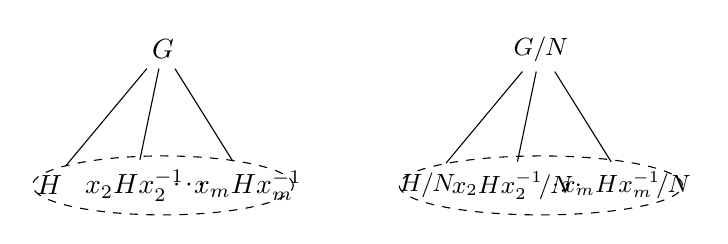
\begin{tikzpicture}[scale=.6]    
    \begin{scope}[shift={(0,0)},scale=1.2,yscale=.8]
      \tikzstyle{every node}=[font=\normalsize]
      \node (G) at (0,4) {$G$};
      \node (H) at (-2,1) {$H$};
      \node (H2) at (-.5,1) {$x_2Hx_2^{-1}$};
      \node (H3) at (.5,1) {$\cdots$};
      \node (Hl) at (1.5,1) {$x_m Hx_m^{-1}$};
      \draw (G)--(H); %node[above left,pos=.5] {\footnotesize $n$};
      \draw (G) -- (H2); \draw (G) -- (Hl);
      \draw[dashed] (0,1) circle [x radius=2.3cm, y radius=.65cm];
    \end{scope}
    %%
    \begin{scope}[shift={(8,0)},scale=1.2,yscale=.8]
      \tikzstyle{every node}=[font=\small]
      \node (G) at (0,4) {$G/N$};
      \node (H) at (-2,1) {$H/N$};
      \node (H2) at (-.5,1) {$x_2Hx_2^{-1}\!/N$};
      \node (H3) at (.5,1) {$\cdots$};
      \node (Hl) at (1.5,1) {$x_m Hx_m^{-1}\!/N$};
      \draw (G)--(H); %node[above left,pos=.5] {\footnotesize $n$};
      \draw (G) -- (H2); \draw (G) -- (Hl);
      \draw[dashed] (0,1) circle [x radius=2.5cm, y radius=.65cm];
    \end{scope}
  \end{tikzpicture}
  \]
  
  \medskip\Pause
  
  Let's apply that to find the conjugacy classes of $C_4\!\rtimes\!C_4$
  by inspection alone.
  %%
  %% Correspondence thoerem, part 5, C_4\rtimes C_4
  %%
  \[
  \begin{tikzpicture}[shorten >= -2pt, shorten <= -2pt,xscale=1.2,scale=.7]
    \tikzstyle{every node}=[font=\footnotesize]
    \begin{scope}[shift={(0,0)},scale=.75,yscale=1.6,scale=.9]
      \node (G) at (0,4) {$C_4\!\rtimes\!C_4$};
      \node (C4xC2-1) at (-1.5,3) {$C_4\!\times\!C_2$};
      \node (C4xC2-2) at (0,3) {$C_4\!\times\!C_2$};
      \node (C4xC2-3) at (1.5,3) {$C_4\!\times\!C_2$};
      \node (C4-1) at (-3,2) {$C_4$};
      \node (C4-2) at (-2,2) {$C_4$};
      \node (C4-3) at (-1.33,2) {$C_4$};
      \node (C4-4) at (-.67,2) {$C_4$};
      \node [faded] (C4-5) at (1.5,2) {$C_4$};
      \node [faded] (C4-6) at (3,2) {$C_4$};
      \node (V4) at (0,2) {$V_4$};
      \node (C2-1) at (-1.5,1) {$C_2$};
      \node [faded] (C2-2) at (0,1) {$C_2$};
      \node [faded] (C2-3) at (1.5,1) {$C_2$};
      \node [faded] (1) at (0,0) {$C_1$};
      \draw [thick] (G) to (C4xC2-1);
      \draw [thick] (G) to (C4xC2-2);
      \draw [thick] (G) to (C4xC2-3);
      \draw [thick] (C4xC2-1) to (C4-1);
      \draw [thick] (C4xC2-1) to (C4-2);
      \draw [thick] (C4xC2-1) to (V4); 
      \draw [thick] (C4xC2-2) to (C4-3);
      \draw [thick] (C4xC2-2) to (C4-4);
      \draw [thick] (C4xC2-2) to (V4); 
      \draw [faded] (C4xC2-3) to (C4-5);
      \draw [faded] (C4xC2-3) to (C4-6);
      \draw [thick] (C4xC2-3) to (V4);
      \draw [thick] (C4-1) to (C2-1); \draw [thick] (C4-2) to (C2-1);
      \draw [thick] (C4-3) to (C2-1); \draw [thick] (C4-4) to (C2-1);
      \draw [thick] (V4) to (C2-1); 
      \draw [faded] (V4) to (C2-2); \draw [faded] (V4) to (C2-3);
      \draw [faded] (C4-5) to (C2-3); \draw [faded] (C4-6) to (C2-3);
      \draw [faded] (C2-1) to (1); 
      \draw [faded] (C2-2) to (1); 
      \draw [faded] (C2-3) to (1);
    \end{scope}
    %%
    \begin{scope}[shift={(4.75,0)},scale=.75,yscale=1.6,scale=.9]
      \node (G) at (0,4) {$C_4\!\rtimes\!C_4$};
      \node (C4xC2-1) at (-1.5,3) {$C_4\!\times\!C_2$};
      \node (C4xC2-2) at (0,3) {$C_4\!\times\!C_2$};
      \node (C4xC2-3) at (1.5,3) {$C_4\!\times\!C_2$};
      \node [faded] (C4-1) at (-3,2) {$C_4$};
      \node [faded] (C4-2) at (-2,2) {$C_4$};
      \node [faded] (C4-3) at (-1.33,2) {$C_4$};
      \node [faded] (C4-4) at (-.67,2) {$C_4$};
      \node [faded] (C4-5) at (1.5,2) {$C_4$};
      \node [faded] (C4-6) at (3,2) {$C_4$};
      \node (V4) at (0,2) {$V_4$};
      \node [faded] (C2-1) at (-1.5,1) {$C_2$};
      \node (C2-2) at (0,1) {$C_2$};
      \node [faded] (C2-3) at (1.5,1) {$C_2$};
      \node [faded] (1) at (0,0) {$C_1$};
      \draw [thick] (G) to (C4xC2-1); \draw [thick] (G) to (C4xC2-2);
      \draw [thick] (G) to (C4xC2-3);
      \draw [faded] (C4xC2-1) to (C4-1);
      \draw [faded] (C4xC2-1) to (C4-2);
      \draw [thick] (C4xC2-1) to (V4);
      \draw [faded] (C4xC2-2) to (C4-3);
      \draw [faded] (C4xC2-2) to (C4-4);
      \draw [thick] (C4xC2-2) to (V4); 
      \draw [faded] (C4xC2-3) to (C4-5);
      \draw [faded] (C4xC2-3) to (C4-6);
      \draw [thick] (C4xC2-3) to (V4);
      \draw [faded] (C4-1) to (C2-1); \draw [faded] (C4-2) to (C2-1);
      \draw [faded] (C4-3) to (C2-1); \draw [faded] (C4-4) to (C2-1);
      \draw [faded] (V4) to (C2-1);
      \draw [thick] (V4) to (C2-2); 
      \draw [faded] (V4) to (C2-3);
      \draw [faded] (C4-5) to (C2-3); \draw [faded] (C4-6) to (C2-3);
      \draw [faded] (C2-1) to (1); \draw [faded] (C2-2) to (1); 
      \draw [faded] (C2-3) to (1);
    \end{scope}
    %%
    \begin{scope}[shift={(9.5,0)},scale=.75,yscale=1.6,scale=.9]
      \node (G) at (0,4) {$C_4\!\rtimes\!C_4$};
      \node (C4xC2-1) at (-1.5,3) {$C_4\!\times\!C_2$};
      \node (C4xC2-2) at (0,3) {$C_4\!\times\!C_2$};
      \node (C4xC2-3) at (1.5,3) {$C_4\!\times\!C_2$};
      \node [faded] (C4-1) at (-3,2) {$C_4$};
      \node [faded] (C4-2) at (-2,2) {$C_4$};
      \node [faded] (C4-3) at (-1.33,2) {$C_4$};
      \node [faded] (C4-4) at (-.67,2) {$C_4$};
      \node (C4-5) at (1.5,2) {$C_4$};
      \node (C4-6) at (3,2) {$C_4$};
      \node (V4) at (0,2) {$V_4$};
      \node [faded] (C2-1) at (-1.5,1) {$C_2$};
      \node [faded] (C2-2) at (0,1) {$C_2$};
      \node (C2-3) at (1.5,1) {$C_2$};
      \node [faded] (1) at (0,0) {$C_1$};
      \draw [thick] (G) to (C4xC2-1);
      \draw [thick] (G) to (C4xC2-2); \draw [thick] (G) to (C4xC2-3);
      \draw [faded] (C4xC2-1) to (C4-1);
      \draw [faded] (C4xC2-1) to (C4-2);
      \draw [thick] (C4xC2-1) to (V4);
      \draw [faded] (C4xC2-2) to (C4-3);
      \draw [faded] (C4xC2-2) to (C4-4);
      \draw [thick] (C4xC2-2) to (V4); 
      \draw [thick] (C4xC2-3) to (C4-5);
      \draw [thick] (C4xC2-3) to (C4-6);
      \draw [thick] (C4xC2-3) to (V4);
      \draw [faded] (C4-1) to (C2-1); \draw [faded] (C4-2) to (C2-1);
      \draw [faded] (C4-3) to (C2-1); \draw [faded] (C4-4) to (C2-1);
      \draw [faded] (V4) to (C2-1); \draw [faded] (V4) to (C2-2); 
      \draw [thick] (V4) to (C2-3);
      \draw [thick] (C4-5) to (C2-3); \draw [thick] (C4-6) to (C2-3);
      \draw [faded] (C2-1) to (1); \draw [faded] (C2-2) to (1); 
      \draw [faded] (C2-3) to (1);
    \end{scope}
  \end{tikzpicture}
  \]
  
\end{frame}

%%====================================================================

\begin{frame}{The correspondence theorem: subgroups of quotients} %\Pause
  
  Let's prove the first (main) part of the correspondence theorem.
  
  \begin{block}{Correspondence theorem (first part)}
    The subgroups of the quotient $G/N$ are quotients of the
    subgroup $H\leq G$ that contain $N$.
  \end{block}
  
  \begin{exampleblock}{Proof}
    Let $S$ be a subgroup of $G/N$. \Pause Then $S$ is a collection of
    cosets, i.e.,
    \[
    S=\big\{hN\mid h\in H\big\},
    \]
    for some \Balert{subset} $H\subseteq G$. \Pause We just need to
    show that $H$ is a subgroup. \medskip\pause

    We'll use the \Balert{one-step subgroup test}: take
    $h_1N,\,h_2N\in S$. \Pause Then $S$ must also contain
    \begin{equation}\label{eqn:H/N}
    (h_1N)(h_2N)^{-1}=(h_1N)(h_2^{-1}N)=(h_1h_2^{-1})N.
    \end{equation}
    That is, $h_1h_2^{-1}\in H$, which means that $H$ is a
    subgroup. $\hfill\checkmark$ \medskip\pause

    Conversely, suppose that $N\leq H\leq G$. \Pause The one-step subgroup
    test shows that $H/N\leq G/N$; see Eq.~\eqref{eqn:H/N}. $\hfill\Box$
  \end{exampleblock}
  
  \smallskip\Pause
  
  The other parts are straightforward and will be left as exercises.
\end{frame}

%%====================================================================

\begin{frame}{The ``subgroup'' and ``quotient'' operations commute} 
  
  \begin{alertblock}{Key idea}
    The \Balert{quotient of a subgroup} is just the \Balert{subgroup
      of the quotient}.
  \end{alertblock}

  \medskip\Pause
  
  \textbf{Example}: Consider the group $G=\SL_2(\Z_3)$.
  %%
  %% Quotient of a subgroup of SL_2(Z_3)
  %%
  \[
  \hspace*{-2mm}
  \begin{tikzpicture}[node distance=1cm,shorten >= -2pt, shorten <= -2pt,scale=.6]
    %%
    \begin{scope}[shift={(0,0)}]
      \tikzstyle{every node}=[font=\footnotesize]
      \node (1) {$\<1\>$};
      \node (a3) at (-2.5,2) {$\<a^3\>$};
      \node (a2) at (.9,3) {$\<a^2\>$};
      \node (b2) at (2,3) {$\<b^2\>$};
      \node (abab) at (3.1,3) {$\<(ab)^2\>$};
      \node (baba) at (4.35,3) {$\<(ba)^2\>$};
      \node (a2b) at (-3.75,4) {$\<a^2b\>$};
      \node (aba) at (-2.5,4) {$\<aba\>$};
      \node (ab2) at (-1.25,4) {$\<ab^2\>$};
      \node (a) at (.5,5) {$\<a\>$};
      \node (b) at (1.6,5) {$\<b\>$};
      \node (ab) at (2.7,5) {$\<ab\>$};
      \node (ba) at (3.95,5) {$\<ba\>$};
      \node (a2b-ab2) at (-2.5,6) {$\<a^2b,ab^2\>$};
      \node (G) at (0,8) {$G=\<a,b\>$};
      \draw (1) -- (a3);
      \draw (1) -- (a2);
      \draw (1) -- (b2);
      \draw (1) -- (abab);
      \draw (1) -- (baba);
      \draw (a3) -- (a2b);
      \draw (a3) -- (aba);
      \draw (a3) -- (ab2);
      \draw (a3) -- (a);
      \draw (a3) -- (b);
      \draw (a3) -- (ab);
      \draw (a3) -- (ba);
      \draw (a2) -- (a);
      \draw (b2) -- (b);
      \draw (abab) -- (ab);
      \draw (baba) -- (ba);
      \draw (a2b) -- (a2b-ab2);
      \draw (aba) -- (a2b-ab2);
      \draw (ab2) -- (a2b-ab2);
      \draw (G) -- (a2b-ab2);
      \draw (G) -- (a);
      \draw (G) -- (b);
      \draw (G) -- (ab);
      \draw (G) -- (ba);
    \end{scope}
    %%
    \begin{scope}[shift={(10,0)}]
      \tikzstyle{every node}=[font=\footnotesize]
      \node (1) at (-2.5,0) {\color{faded}$\<1\>$};
      \node (a3) at (-2.5,2) {$\<a^3\>$};
      \node (a2b) at (-3.75,4) {$\<a^2b\>$};
      \node (aba) at (-2.5,4) {$\<aba\>$};
      \node (ab2) at (-1.25,4) {$\<ab^2\>$};
      \node (a2b-ab2) at (-2.5,6) {$\<a^2b,ab^2\>$};
      \draw[faded] (1) -- (a3);
      \draw (a3) -- (a2b);
      \draw (a3) -- (aba);
      \draw (a3) -- (ab2);
      \draw (a2b) -- (a2b-ab2);
      \draw (aba) -- (a2b-ab2);
      \draw (ab2) -- (a2b-ab2);
      \node at (-2.5,7.5) {\normalsize subgroup $\bm{H\cong Q_8}$};
    \end{scope}
    %%
    \begin{scope}[shift={(15,0)}]
      \tikzstyle{every node}=[font=\scriptsize]
      \node (a3) at (-2.5,2) {$\<a^3\>/N$};
      \node (a2b) at (-3.75,4) {\hspace{-2mm}$\<a^2b\>/N$};
      \node (aba) at (-2.5,4) {$\<aba\>/N$};
      \node (ab2) at (-1.25,4) {$\<ab^2\>/N$};
      \node (a2b-ab2) at (-2.5,6) {\hspace{2mm}$\<a^2b,ab^2\>/N$};
      \draw (a3) -- (a2b);
      \draw (a3) -- (aba);
      \draw (a3) -- (ab2);
      \draw (a2b) -- (a2b-ab2);
      \draw (aba) -- (a2b-ab2);
      \draw (ab2) -- (a2b-ab2);
      \node at (-2.5,7.5) {\normalsize $\bm{H/N\cong V_4}$};
      \node at (-2.5,1) {\normalsize ``\emph{quotient of the subgroup}''};
    \end{scope}
  \end{tikzpicture}
  \]
  
\end{frame}

%%====================================================================

\begin{frame}{The ``subgroup'' and ``quotient'' operations commute} 
  
  \begin{alertblock}{Key idea}
    The \Balert{quotient of a subgroup} is just the \Balert{subgroup
      of the quotient}.
  \end{alertblock}
  
  \medskip
  
  \textbf{Example}: Consider the group $G=\SL_2(\Z_3)$. %\vspace{-4mm}
  %%
  %% Subgroup of a quotient of SL_2(Z_3)
  %%
  \[
  \hspace*{-2mm}
  \begin{tikzpicture}[node distance=1cm,shorten >= -2pt, shorten <= -2pt,scale=.6]
    \begin{scope}[shift={(0,0)}]
      \tikzstyle{every node}=[font=\tiny]
      \node at (-3.5,7.5) {\normalsize quotient $\bm{G/N\cong A_4}$};
      \node (1) {\color{faded}$\<1\>$};
      \node (a3) at (-2.5,2) {$\<a^3\>/N$};
      \node (a2) at (.9,3) {\color{faded}$\<a^2\>$};
      \node (b2) at (2,3) {\color{faded}$\<b^2\>$};
      \node (abab) at (3.1,3) {\color{faded}$\<(ab)^2\>$};
      \node (baba) at (4.35,3) {\color{faded}$\<(ba)^2\>$};
      \node (a2b) at (-3.75,4) {$\<a^2b\>/N$};
      \node (aba) at (-2.5,4) {$\<aba\>/N$};
      \node (ab2) at (-1.25,4) {$\<ab^2\>/N$};
      \node (a) at (.5,5) {$\<a\>/N$};
      \node (b) at (1.6,5) {$\<b\>/N$};
      \node (ab) at (2.7,5) {$\<ab\>/N$};
      \node (ba) at (3.95,5) {$\<ba\>/N$};
      \node (a2b-ab2) at (-2.5,6) {$\<a^2b,ab^2\>/N$};
      \node (G) at (0,8) {$\<a,b\>/N$};
      \draw[faded] (1) -- (a3);
      \draw[faded] (1) -- (a2);
      \draw[faded] (1) -- (b2);
      \draw[faded] (1) -- (abab);
      \draw[faded] (1) -- (baba);
      \draw (a3) -- (a2b);
      \draw (a3) -- (aba);
      \draw (a3) -- (ab2);
      \draw (a3) -- (a);
      \draw (a3) -- (b);
      \draw (a3) -- (ab);
      \draw (a3) -- (ba);
      \draw[faded] (a2) -- (a);
      \draw[faded] (b2) -- (b);
      \draw[faded] (abab) -- (ab);
      \draw[faded] (baba) -- (ba);
      \draw (a2b) -- (a2b-ab2);
      \draw (aba) -- (a2b-ab2);
      \draw (ab2) -- (a2b-ab2);
      \draw (G) -- (a2b-ab2);
      \draw (G) -- (a);
      \draw (G) -- (b);
      \draw (G) -- (ab);
      \draw (G) -- (ba);
    \end{scope}
    %%
    \begin{scope}[shift={(11,0)}]
      \tikzstyle{every node}=[font=\tiny]
      \node at (-2.5,7.5) {\normalsize$\bm{V_4\cong H/N\leq G/N}$};
      \node (a3) at (-2.5,2) {$\<a^3\>/N$};
      \node (a2b) at (-3.75,4) {$\<a^2b\>/N$};
      \node (aba) at (-2.5,4) {$\<aba\>/N$};
      \node (ab2) at (-1.25,4) {$\<ab^2\>/N$};
      \node (a2b-ab2) at (-2.5,6) {$\<a^2b,ab^2\>/N$};
      \draw (a3) -- (a2b);
      \draw (a3) -- (aba);
      \draw (a3) -- (ab2);
      \draw (a2b) -- (a2b-ab2);
      \draw (aba) -- (a2b-ab2);
      \draw (ab2) -- (a2b-ab2);
      \node at (-2.5,1) {\normalsize ``\emph{subgroup of the quotient}''};
    \end{scope}
  \end{tikzpicture}
  \]
  
\end{frame}

%%====================================================================

\begin{frame}{The fraction theorem: quotients of quotients} \smallskip
  
  The correspondence theorem characterizes the \Balert{subgroup
    structure} of the quotient $G/N$. \medskip\Pause

  Every subgroup of $G/N$ is of the form $H/N$, where $N\leq H\leq
  G$. \medskip\Pause

  Moreover, if $H\normaleq G$, then
  $H/N\normaleq G/N$. \Pause In this case, we can ask:
  \[
  \text{\emph{What is the quotient group $(G/N)/(H/N)$ isomorphic to?}}
  \]
  
  \vspace{-2mm}\Pause
  
  \begin{block}{Fraction theorem}
    Given a chain $N\leq H\leq G$ of normal subgroups of $G$,
    \[
    (G/N)/(H/N)\cong G/H.
    \]
  \end{block}
  
  \vspace{-4mm}

  %%
  %% Fraction thoerem, SA_8 lattices
  %%
  \[
  \begin{tikzpicture}[node distance=1cm,shorten >= -2pt, shorten <= -2pt,scale=.5]
    \tikzstyle{every node}=[font=\footnotesize]
    \begin{scope}[shift={(0,0)}]
      \node (G) at (3.5,6) {$\hspace{5mm}\SA_8\!=\!G$};
      \node(rs) at (3.5,4.5) {$\<rs\>$};
      \node(r2-s) at (1.75,4.5) {$\<r^2,s\>$};
      \node(r) at (5.25,4.5) {$\<r\>$};
      \node(r4-s) at (0,3) {$\<r^4,s\>$};
      \node(r2s) at (1.75,3) {$\<r^2s\>$};
      \node(r2) at (3.5,3) {$\hspace{6mm}\<r^2\>\!=\!H$};
      \node(s) at (-1.75,1.5) {\color{faded}$\<s\>$};
      \node(r4s) at (0,1.5) {\color{faded}$\<r^4s\>$};
      \node(r4) at (1.75,1.5) {$\hspace{6mm}\<r^4\>\!=\!N$};
      \node(1) at (0,0) {\color{faded}$\<1\>$};
      \draw[faded] (1) -- (s);
      \draw[faded] (1) -- (r4s);
      \draw[faded] (1) -- (r4);
      \draw[faded] (s) -- (r4-s);
      \draw[faded] (r4s) -- (r4-s);
      \draw [thick] (r4) -- (r4-s); 
      \draw [thick] (r4) -- (r2s);
      \draw [thick] (r4) -- (r2);
      \draw [thick] (r4-s) -- (r2-s);
      \draw [thick] (r2s) -- (r2-s);
      \draw [thick] (r2) -- (r2-s);
      \draw [thick] (r2) -- (r);
      \draw [thick] (r2) -- (rs);
      \draw [thick] (r2-s) -- (G);
      \draw [thick] (r) -- (G);
      \draw [thick] (rs) -- (G);
    \end{scope}
    %%
    \begin{scope}[shift={(7,0)}]
      \node(G) at (3.5,6) {$G/N$};
      \node(rs) at (3.5,4.5) {$\<rs\>/N$};
      \node(r2-s) at (1.75,4.5) {$\<r^2,s\>/N$};
      \node(r) at (5.25,4.5) {$\<r\>/N$};
      \node(r4-s) at (0,3) {\color{faded}$\<r^4,s\>\!/N$};
      \node(r2s) at (1.75,3) {\color{faded}$\<r^2s\>\!/N$};
      \node(r2) at (3.5,3) {$\<r^2\>/N$};
      \node(r4) at (1.75,1.5) {\color{faded}$\<r^4\>/N$};
      \draw[faded] (r4) -- (r4-s);
      \draw[faded] (r4) -- (r2s);
      \draw[faded] (r4) -- (r2);
      \draw[faded] (r4-s) -- (r2-s);
      \draw[faded] (r2s) -- (r2-s);
      \draw [thick] (r2) -- (r2-s);
      \draw [thick] (r2) -- (r);
      \draw [thick] (r2) -- (rs);
      \draw [thick] (r2-s) -- (G);
      \draw [thick] (r) -- (G);
      \draw [thick] (rs) -- (G);
    \end{scope}
    %%
    \begin{scope}[shift={(14.75,0)}]
      \node(G) at (3.5,6) {$G/H$};
      \node(rs) at (3.5,4.5) {$\<rs\>\!/H$};
      \node(r2-s) at (1.75,4.5) {$\<r^2\!,s\>\!/H$};
      \node(r) at (5.25,4.5) {$\<r\>\!/H$};
      \node(r2) at (3.5,3) {$\<r^2\>\!/H$};
      %%
      \node(r4-s) at (0,3) {\color{faded}$\<r^4,s\>$};
      \node(r2s) at (1.75,3) {\color{faded}$\<r^2s\>$};
      \node(s) at (-1.75,1.5) {\color{faded}$\<s\>$};
      \node(r4s) at (0,1.5) {\color{faded}$\<r^4s\>$};
      \node(r4) at (1.75,1.5) {\color{faded}$\<r^4\>$};
      \node(1) at (0,0) {\color{faded}$\<1\>$};
      \draw[faded] (r4) -- (r4-s);
      \draw[faded] (r4) -- (r2s);
      \draw[faded] (r4) -- (r2);
      \draw[faded] (r4-s) -- (r2-s);
      \draw[faded] (r2s) -- (r2-s);
      \draw[faded] (1) -- (s);
      \draw[faded] (1) -- (r4s);
      \draw[faded] (1) -- (r4);
      \draw[faded] (s) -- (r4-s);
      \draw[faded] (r4s) -- (r4-s);
      \draw [thick] (r2) -- (r2-s);
      \draw [thick] (r2) -- (r);
      \draw [thick] (r2) -- (rs);
      \draw [thick] (r2-s) -- (G);
      \draw [thick] (r) -- (G);
      \draw [thick] (rs) -- (G);
    \end{scope}
  \end{tikzpicture}
  \]
  
\end{frame}

%%====================================================================

\begin{frame}{The fraction theorem: quotients of quotients} %\smallskip
    
  \begin{block}{Fraction theorem}
    Given a chain $N\leq H\leq G$ of normal subgroups of $G$, \vspace{-1mm}
    \[
    (G/N)/(H/N)\cong G/H.
    \]
  \end{block}

  \vspace{-3mm}

  %% Three subgroup lattices of quotients of G/N showing the fraction thm
  \[
  \begin{tikzpicture}[node distance=1cm,shorten >= -2pt, shorten <= -2pt,scale=.45,xscale=1]
    \begin{scope}[shift={(0,0)}]
     \tikzstyle{every node}=[font=\footnotesize]
      \node(G) at (3.5,6) {$\hspace{5mm}\SA_8\!=\!G$};
      \node(rs) at (3.5,4.5) {$\<rs\>$};
      \node(r2-s) at (1.75,4.5) {$\<r^2,s\>$};
      \node(r) at (5.25,4.5) {$\<r\>$};
      \node(r4-s) at (0,3) {\hspace{-1mm}$\<r^4,s\>$};
      \node(r2s) at (1.75,3) {$\<r^2s\>$};
      \node(r2) at (3.5,3) {\hspace{4mm}$\<r^2\>\!=\!\Balert{H}$};
      \node(s) at (-1.75,1.5) {\color{faded}$\<s\>$};
      \node(r4s) at (0,1.5) {\color{faded}$\<r^4s\>$};
      \node(r4) at (1.75,1.5) {\hspace{4mm}$\<r^4\>\!=\!\Alert{N}$};
      \node(1) at (0,0) {\color{faded}$\<1\>$};
      \draw[faded] (1) -- (s);
      \draw[faded] (1) -- (r4s);
      \draw[faded] (1) -- (r4);
      \draw[faded] (s) -- (r4-s);
      \draw[faded] (r4s) -- (r4-s);
      \draw[thick] (r4) -- (r4-s);
      \draw[thick] (r4) -- (r2s);
      \draw[thick] (r4) -- (r2);
      \draw[thick] (r4-s) -- (r2-s);
      \draw[thick] (r2s) -- (r2-s);
      \draw[thick] (r2) -- (r2-s);
      \draw[thick] (r2) -- (r);
      \draw[thick] (r2) -- (rs);
      \draw[thick] (r2-s) -- (G);
      \draw[thick] (r) -- (G);
      \draw[thick] (rs) -- (G);
    \end{scope}
    %%
    \begin{scope}[shift={(7.5,0)}]
     \tikzstyle{every node}=[font=\footnotesize]
      \node(G) at (3.5,6) {$G\!/\!N$};
      \node(rs) at (3.5,4.5) {$\<rs\>\!/\!N$};
      \node(r2-s) at (1.75,4.5) {$\<r^2\!,s\>\!/\!N$};
      \node(r) at (5.25,4.5) {$\<r\>\!/\!N$};
      \node(r4-s) at (0,3) {\hspace{-2mm}$\<r^4,s\>\!/\!N$};
      \node(r2s) at (1.75,3) {$\<r^2s\>\!/\!N$};
      \node(r2) at (3.5,3) {\hspace{8mm}$\<r^2\>\!/\!N\!=\!\Balert{H\!/\!N}$};
      \node(r4) at (1.75,1.5) {$N\!/\!N$};
      \draw[thick] (r4) -- (r4-s);
      \draw[thick] (r4) -- (r2s);
      \draw[thick] (r4) -- (r2);
      \draw[thick] (r4-s) -- (r2-s);
      \draw[thick] (r2s) -- (r2-s);
      \draw[thick] (r2) -- (r2-s);
      \draw[thick] (r2) -- (r);
      \draw[thick] (r2) -- (rs);
      \draw[thick] (r2-s) -- (G);
      \draw[thick] (r) -- (G);
      \draw[thick] (rs) -- (G);
    \end{scope}
      \begin{scope}[shift={(15,0)}]
      \tikzstyle{every node}=[font=\footnotesize]
      \node(G) at (3.5,6) {$C_4\!\times\!C_2$};
      \node(rs) at (3.5,4.5) {$C_4$};
      \node(r2-s) at (1.75,4.5) {$V_4$};
      \node(r) at (5.25,4.5) {$C_4$};
      \node(r4-s) at (0,3) {$C_2$};
      \node(r2s) at (1.75,3) {$C_2$};
      \node(r2) at (3.5,3) {$C_2$};
      \node(r4) at (1.75,1.5) {$C_1$};
      \draw[thick] (r4) -- (r4-s);
      \draw[thick] (r4) -- (r2s);
      \draw[thick] (r4) -- (r2);
      \draw[thick] (r4-s) -- (r2-s);
      \draw[thick] (r2s) -- (r2-s);
      \draw[thick] (r2) -- (r2-s);
      \draw[thick] (r2) -- (r);
      \draw[thick] (r2) -- (rs);
      \draw[thick] (r2-s) -- (G);
      \draw[thick] (r) -- (G);
      \draw[thick] (rs) -- (G);
    \end{scope}
  \end{tikzpicture}
  \]

  \vspace{-7mm}

  %% Four subgroup lattices of quotients of G/N showing the fraction thm
  \[
  \begin{tikzpicture}[scale=.45,xscale=1,shorten >= -2pt, shorten <= -2pt]
    %%
    \begin{scope}[shift={(0,0)}]
    \tikzstyle{every node}=[font=\footnotesize]
      \node(G) at (3.5,6) {$G\!/\!N$};
      \node(rs) at (3.5,4.5) {$\<rs\>\!/\!N$};
      \node(r2-s) at (1.75,4.5) {$\<r^2,s\>\!/\!N$};
      \node(r) at (5.25,4.5) {$\<r\>\!/\!N$};
      \node[faded] (r4-s) at (0,3) {$\<r^4\!,s\>\!/\!N$};
      \node[faded] (r2s) at (1.75,3) {$\<r^2s\>\!/\!N$};
      \node (r2) at (3.5,3) {\hspace{7mm}$\<r^2\>\!/\!N\!=\!\Balert{H\!/\!N}$};
      \node[faded] (r4) at (1.75,1.5) {$\<r^4\>\!/\!N$};
      \draw[f] (r4) -- (r4-s);
      \draw[f] (r4) -- (r2s);
      \draw[f] (r4) -- (r2);
      \draw[f] (r4-s) -- (r2-s);
      \draw[f] (r2s) -- (r2-s);
      \draw[thick] (r2) -- (r2-s);
      \draw[thick] (r2) -- (r);
      \draw[thick] (r2) -- (rs);
      \draw[thick] (r2-s) -- (G);
      \draw[thick] (r) -- (G);
      \draw[thick] (rs) -- (G);
    \end{scope}
    %%
    \begin{scope}[shift={(5.75,0)},shorten >= -2pt, shorten <= -2pt]
      \tikzstyle{every node}=[font=\small]
      \node(G) at (3.5,6) {$\frac{G\!/\!N}{H\!/\!N}$};
      \node(rs) at (3.5,4.5) {$\frac{\<rs\>\!/\!N}{H\!/\!N}$};
      \node(r2-s) at (1.75,4.5) {$\frac{\<r^2\!,s\>\!/\!N}{H\!/\!N}$};
      \node(r) at (5.25,4.5) {$\frac{\<r\>\!/\!N}{H\!/\!N}$};
      \node(r2) at (3.5,3) {$\frac{H\!/\!N}{H\!/\!N}$};
      \draw[thick,shorten >= -5pt, shorten <= -5pt] (r2) -- (r2-s);
      \draw[thick,shorten >= -5pt, shorten <= -5pt] (r2) -- (r);
      \draw[thick] (r2) -- (rs);
      \draw[thick,shorten >= -5pt, shorten <= -5pt] (r2-s) -- (G);
      \draw[thick,shorten >= -5pt, shorten <= -5pt] (r) -- (G);
      \draw[thick] (rs) -- (G);
    \end{scope}
    %%
    \begin{scope}[shift={(11.5,0)}]
    \tikzstyle{every node}=[font=\footnotesize]
      \node(G) at (3.5,6) {$G\!/\!H$};
      \node(rs) at (3.5,4.5) {$\<rs\>\!/\!H$};
      \node(r2-s) at (1.75,4.5) {$\<r^2,s\>\!/\!H$};
      \node(r) at (5.25,4.5) {$\<r\>\!/\!H$};
      \node(r2) at (3.5,3) {$H\!/\!H$};
      %%
      \draw[thick] (r2) -- (r2-s);
      \draw[thick] (r2) -- (r);
      \draw[thick] (r2) -- (rs);
      \draw[thick] (r2-s) -- (G);
      \draw[thick] (r) -- (G);
      \draw[thick] (rs) -- (G);
    \end{scope}
    %%
    \begin{scope}[shift={(17,0)}]
    \tikzstyle{every node}=[font=\footnotesize]
      \node(G) at (3.5,6) {$V_4$};
      \node(rs) at (3.5,4.5) {$C_2$};
      \node(r2-s) at (1.75,4.5) {$C_2$};
      \node(r) at (5.25,4.5) {$C_2$};
      \node(r2) at (3.5,3) {$C_1$};
      \draw[thick] (r2) -- (r2-s);
      \draw[thick] (r2) -- (r);
      \draw[thick] (r2) -- (rs);
      \draw[thick] (r2-s) -- (G);
      \draw[thick] (r) -- (G);
      \draw[thick] (rs) -- (G);
    \end{scope}
    %%
  \end{tikzpicture}
  \]

\end{frame}

%%====================================================================

\begin{frame}{The fraction theorem: quotients of quotients} \smallskip
  
  Let's continue our example of the semiabelian group
  $G=\SA_8=\<r,s\>$. \smallskip
  
  %%%%%%%%%%%%%%%%%%%%%%%%%%%%%%%%%%%%%%%%%%%%

  %%
  %% Fraction thoerem, SA_8 (shoeboxes)
  %%
  \[
  \begin{tikzpicture}[xscale=.9,scale=.7]
    %%%%%%%%%%%%%
    \begin{scope}[shift={(0,0)}]
      \tikzstyle{every node}=[font=\footnotesize,anchor=south]
      \begin{scope}[shift={(0,3.5)}]
        \draw[thick,rounded corners] (0,0) rectangle (4,3.2);
        \draw[thick,eBlue,rounded corners] (.1,.1) rectangle (1.95,1.55);     
        \draw[thick,eRed,rounded corners] (.2,.2) rectangle (1.85,.2+.575);
        %% 
        \node at (.5,2.45) {$r^3$};
        \node at (1.5,2.45) {$r^7$};
        \node at (.5,1.75) {$r$};
        \node at (1.5,1.75) {$r^5$};
        %%
        \node at (2.5,2.45) {$r^3s$};
        \node at (3.45,2.45) {$r^7s$};
        \node at (2.5,1.75) {$rs$};
        \node at (3.45,1.75) {$r^5s$};
        %%
        \node at (.5,.9) {$r^2$};
        \node at (1.5,.9) {$r^6$};
        \node at (.5,.2) {$1$};
        \node at (1.5,.2) {$r^4$};
        %%
        \node at (2.5,.9) {$r^2s$};
        \node at (3.45,.9) {$r^6s$};
        \node at (2.5,.2) {$s$};
        \node at (3.45,.2) {$r^4s$};
        %% 
        \node at (2,-.75) {\small $\Alert{N}\leq \Balert{H}\leq G$};
      \end{scope}
    \end{scope}
    %%%%%%%%%%%%%%%%%%%%%%%%%%%%%%%
    \begin{scope}[shift={(5.5,0)}]
      \tikzstyle{every node}=[font=\footnotesize,anchor=south,faded]
      %%
      \begin{scope}[shift={(0,3.5)}]
        \draw[thick,rounded corners] (0,0) rectangle (4,3.2);
        %% (upper-left)
        \draw[thick,xBlue,fill=cosetBlue,rounded corners] (.1,1.65) rectangle (1.95,3.1);
        \draw[thick,xRed,fill=cosetRed,rounded corners] (.2,3-.575) rectangle (1.85,3);
        \draw[thick,xRed,fill=cosetRed,rounded corners] (.2,1.75) rectangle (1.85,1.75+.575);
        %% (lower-left)
        \draw[thick,xBlue,fill=cosetBlue,rounded corners] (.1,.1) rectangle (1.95,1.55);     
        \draw[thick,xRed,fill=cosetRed,rounded corners] (.2,1.45-.575) rectangle (1.85,1.45);
        \draw[thick,xRed,fill=cosetRed,rounded corners] (.2,.2) rectangle (1.85,.2+.575);
        %% (upper-right)
        \draw[thick,xBlue,fill=cosetBlue,rounded corners] (2.05,1.65) rectangle (3.9,3.1);
        \draw[thick,xRed,fill=cosetRed,rounded corners] (2.15,3-.575) rectangle (3.8,3);
        \draw[thick,xRed,fill=cosetRed,rounded corners] (2.15,1.75) rectangle (3.8,1.75+.575);
        %% (lower-right)
        \draw[thick,xBlue,fill=cosetBlue,rounded corners] (2.05,.1) rectangle (3.9,1.55);   
        \draw[thick,xRed,fill=cosetRed,rounded corners] (2.15,1.45-.575) rectangle (3.8,1.45);
        \draw[thick,xRed,fill=cosetRed,rounded corners] (2.15,.2) rectangle (3.8,.2+.575);
        %% 
        \node at (.5,2.45) {$r^3$};
        \node at (1.5,2.45) {$r^7$};
        \node at (.5,1.75) {$r$};
        \node at (1.5,1.75) {$r^5$};
        %%
        \node at (2.5,2.45) {$r^3s$};
        \node at (3.45,2.45) {$r^7s$};
        \node at (2.5,1.75) {$rs$};
        \node at (3.45,1.75) {$r^5s$};
        %%
        \node at (.5,.9) {$r^2$};
        \node at (1.5,.9) {$r^6$};
        \node at (.5,.2) {$1$};
        \node at (1.5,.2) {$r^4$};
        %%
        \node at (2.5,.9) {$r^2s$};
        \node at (3.45,.9) {$r^6s$};
        \node at (2.5,.2) {$s$};
        \node at (3.45,.2) {$r^4s$};
        %%
        \node at (1,2.45) {\Alert{$\mathbf{r^3N}$}};
        \node at (1,1.77) {\Alert{$\mathbf{rN}$}};
        \node at (3,2.45) {\Alert{$\mathbf{r^3sN}$}};
        \node at (3,1.77) {\Alert{$\mathbf{rsN}$}};
        %%
        \node at (1,.9) {\Alert{$\mathbf{r^2N}$}};
        \node at (1,.22) {\Alert{$\mathbf{N}$}};
        \node at (3,.9) {\Alert{$\mathbf{r^2sN}$}};
        \node at (3,.22) {\Alert{$\mathbf{sN}$}};
        %%
        \node at (2,-.75) {\small\Alert{$G/N=\<rN,sN\>\cong C_4\times C_2$}};
        \node at (2,-1.25) {\small\Balert{$H/N=\<r^2N\>=\{N,r^2N\}\cong C_2$}};
      \end{scope}
    \end{scope}
    %%%%%%%%%%%%%%%%%%%%%%%%%%%%%%%
    \begin{scope}[shift={(11,0)}]
      \tikzstyle{every node}=[font=\footnotesize,anchor=south,faded]
      \begin{scope}[shift={(0,3.5)}]
        \draw[thick,rounded corners] (0,0) rectangle (4,3.2);
        %% (upper-left)
        \draw[thick,xBlue,fill=cosetBlue,rounded corners] (.1,1.65) rectangle (1.95,3.1);
        \draw[thick,xBlue,fill=cosetBlue,rounded corners] (.1,.1) rectangle (1.95,1.55);     
        \draw[thick,xBlue,fill=cosetBlue,rounded corners] (2.05,1.65) rectangle (3.9,3.1);
        \draw[thick,xBlue,fill=cosetBlue,rounded corners] (2.05,.1) rectangle (3.9,1.55);   
        %% 
        \node at (.5,2.45) {$r^3$};
        \node at (1.5,2.45) {$r^7$};
        \node at (.5,1.75) {$r$};
        \node at (1.5,1.75) {$r^5$};
        %%
        \node at (2.5,2.45) {$r^3s$};
        \node at (3.45,2.45) {$r^7s$};
        \node at (2.5,1.75) {$rs$};
        \node at (3.45,1.75) {$r^5s$};
        %%
        \node at (.5,.9) {$r^2$};
        \node at (1.5,.9) {$r^6$};
        \node at (.5,.2) {$1$};
        \node at (1.5,.2) {$r^4$};
        %%
        \node at (2.5,.9) {$r^2s$};
        \node at (3.45,.9) {$r^6s$};
        \node at (2.5,.2) {$s$};
        \node at (3.45,.2) {$r^4s$};
        \node at (1,2.1) {\normalsize\Balert{$\mathbf{rH}$}};
        \node at (1,.55) {\normalsize\Balert{$\mathbf{H}$}};
        \node at (3,2.1) {\normalsize\Balert{$\mathbf{rsH}$}};
        \node at (3,.55) {\normalsize\Balert{$\mathbf{sH}$}};
        %%
        \node at (2,-.75) {\small\Balert{$G/H=\<rH,sH\>\cong V_4$}};
        \node at (2,-1.25) {\small\Balert{$(G/N)/(H/N)\cong G/H$}};
      \end{scope}
    \end{scope}
  \end{tikzpicture}
  \]
  
  %%%%%%%%%%%%%%%%%%%%%%%%%%%%%%%%%%%%%%

  %%
  %% Fraction thoerem, SA_8 (Cayley graphs)
  %%
  \[
  \begin{tikzpicture}[xscale=.95,scale=.6]
    \begin{scope}
      \node at (3.25,2.4) {\large $(G/N)/(H/N)$};
      \tikzstyle{every node}=[font=\footnotesize,anchor=south,faded]
      %%
      \begin{scope}[shift={(0,3.5)}]
        \draw[thick,xBlue,fill=cosetBlue,rounded corners] (0,0) rectangle (2,1.6);
        \draw[thick,fRed,rounded corners,fill=cosetRed] (.1,.1) rectangle (1.9,.75);
        \draw[thick,fRed,rounded corners,fill=cosetRed] (.1,.85) rectangle (1.9,1.5);
        \node at (.5,.9) {$r^3$};
        \node at (1.5,.9) {$r^7$};
        \node at (.5,.15) {$r$};
        \node at (1.5,.15) {$r^5$};
        \node[xRed] at (1,.45) {\normalsize $\mathbf{rN\<r^2N\>}$};
        \draw[ultra thick,eBlue] (2,.8)--(4.5,.8);
      \end{scope}
      %%
      \begin{scope}[shift={(0,0)}]
        \draw[thick,xBlue,fill=cosetBlue,rounded corners] (0,0) rectangle (2,1.6);
        \draw[thick,fRed,rounded corners,fill=cosetRed] (.1,.1) rectangle (1.9,.75);
        \draw[thick,fRed,rounded corners,fill=cosetRed] (.1,.85) rectangle (1.9,1.5);
        \node at (.5,.9) {$r^2$};
        \node at (1.5,.9) {$r^6$};
        \node at (.5,.15) {$1$};
        \node at (1.5,.15) {$r^4$};
        \node[xRed] at (1,.45) {\normalsize $\mathbf{\<r^2N\>}$};
        \draw[ultra thick,eBlue] (2,.8)--(4.5,.8);
        \draw[ultra thick,eRed] (1,1.6)--(1,3.5);
      \end{scope}
      %%
      \begin{scope}[shift={(4.5,3.5)}]
        \draw[thick,xBlue,fill=cosetBlue,rounded corners] (0,0) rectangle (2,1.6);
        \draw[thick,fRed,rounded corners,fill=cosetRed] (.1,.1) rectangle (1.9,.75);
        \draw[thick,fRed,rounded corners,fill=cosetRed] (.1,.85) rectangle (1.9,1.5);
        \node at (.5,.9) {$r^3\!s$};
        \node at (1.5,.9) {$r^7\!s$};
        \node at (.5,.15) {$rs$};
        \node at (1.5,.15) {$r^5\!s$};
        \node[xRed] at (1,.45) {\normalsize $\mathbf{rsN\<r^2N\>}$};
      \end{scope}
      %%
      \begin{scope}[shift={(4.5,0)}]
        \draw[thick,xBlue,fill=cosetBlue,rounded corners] (0,0) rectangle (2,1.6);
        \draw[thick,fRed,rounded corners,fill=cosetRed] (.1,.1) rectangle (1.9,.75);
        \draw[thick,fRed,rounded corners,fill=cosetRed] (.1,.85) rectangle (1.9,1.5);
        \node at (.5,.9) {$r^2\!s$};
        \node at (1.5,.9) {$r^6\!s$};
        \node at (.5,.15) {$s$};
        \node at (1.5,.15) {$r^4\!s$};
        \node[xRed] at (1,.45) {\normalsize $\mathbf{sN\<r^2N\>}$};
        \draw[ultra thick,eRed] (1,1.6)--(1,3.5);
      \end{scope}  
    \end{scope}
    %%%%%%%%%%%%%%%%%%%%%%%%%%%%%%%%%%%%%%%%%%%%%%%%%%%%
    \begin{scope}[shift={(9,0)}]
      \node at (3.25,2.4) {\large $G/H$};
      \tikzstyle{every node}=[font=\footnotesize,anchor=south,faded]
      %%
      \begin{scope}[shift={(0,3.5)}]
        \draw[thick,xBlue,fill=cosetBlue,rounded corners] (0,0) rectangle (2,1.6);
        \node at (.5,.9) {$r^3$};
        \node at (1.5,.9) {$r^7$};
        \node at (.5,.15) {$r$};
        \node at (1.5,.15) {$r^5$};
        \node[xBlue] at (1,.45) {\normalsize $\mathbf{rH}$};
        \draw[ultra thick,eBlue] (2,.8)--(4.5,.8);
      \end{scope}
      %%
      \begin{scope}[shift={(0,0)}]
        \draw[thick,xBlue,fill=cosetBlue,rounded corners] (0,0) rectangle (2,1.6);
        \node at (.5,.9) {$r^2$};
        \node at (1.5,.9) {$r^6$};
        \node at (.5,.15) {$1$};
        \node at (1.5,.15) {$r^4$};
        \node[xBlue] at (1,.45) {\normalsize $\mathbf{H}$};
        \draw[ultra thick,eRed] (1,1.6)--(1,3.5);
        \draw[ultra thick,eBlue] (2,.8)--(4.5,.8);
      \end{scope}
      %%
      \begin{scope}[shift={(4.5,3.5)}]
        \draw[thick,xBlue,fill=cosetBlue,rounded corners] (0,0) rectangle (2,1.6);
        \node at (.5,.9) {$r^3\!s$};
        \node at (1.5,.9) {$r^7\!s$};
        \node at (.5,.15) {$rs$};
        \node at (1.5,.15) {$r^5\!s$};
        \node[xBlue] at (1,.45) {\normalsize $\mathbf{rsH}$};
      \end{scope}
      %%
      \begin{scope}[shift={(4.5,0)}]
        \draw[thick,xBlue,fill=cosetBlue,rounded corners] (0,0) rectangle (2,1.6);
        \node at (.5,.9) {$r^2\!s$};
        \node at (1.5,.9) {$r^6\!s$};
        \node at (.5,.15) {$s$};
        \node at (1.5,.15) {$r^4\!s$};
        \node[xBlue] at (1,.45) {\normalsize $\mathbf{sH}$};
        \draw[ultra thick,eRed] (1,1.6)--(1,3.5);
      \end{scope}  
    \end{scope}
    %%%%%%%%%%%%% 
  \end{tikzpicture}
  \]
      
\end{frame}

%%====================================================================

\begin{frame}{The fraction theorem: quotients of quotients} \smallskip
  
  \begin{block}{Fraction theorem}
    Given a chain $N\leq H\leq G$ of normal subgroups of $G$,
    \[
    (G/N)/(H/N)\cong G/H.
    \]
  \end{block}
  
  \Pause
  
  \begin{exampleblock}{Proof}
    This is tailor-made for the FHT. Define the map
    \[
    \Alert{\phi\colon G/N\longto G/H,\qquad\phi\colon
      gN\longmapsto\Pause gH}.
    \]
    \pause $\bullet$ \underline{\emph{Show $\phi$ is well-defined}}\,:
    Suppose $g_1N=g_2N$. \Pause Then $g_1=g_2n$ for some $n\in
    N$. \Pause But $n\in H$ because $N\leq H$. \Pause Thus,
    $g_1H=g_2H$, \Pause i.e., $\phi(g_1N)=\phi(g_2N)$. $\hfill\checkmark$ 
    
    \medskip\pause
    
    $\bullet$ \underline{\emph{$\phi$ is clearly onto and a
        homomorphism}}. $\hfill\checkmark$
    
    \medskip\pause
    
    $\bullet$ \underline{\emph{Apply the FHT}}:
    \begin{center}
      \renewcommand{\arraystretch}{1.2}
      \begin{tabular}{rcl}
        $\Ker(\phi)$ & $=$ & $\big\{gN\in G/N \mid \phi(gN)=H\big\}$ \\ \Pause
        & $=$ & $\big\{gN\in G/N \mid gH=H\big\}$ \\ \Pause
        & $=$ & $\big\{gN\in G/N\mid g\in H\big\}\Pause=H/N$ \\
      \end{tabular}
    \end{center}
    \Pause By the FHT, $(G/N)/\Ker(\phi)=(G/N)/(H/N)\Pause\cong
    \Image(\phi)\Pause=G/H$. $\hfill\Box$
    
  \end{exampleblock}
  
\end{frame}

%%====================================================================

\begin{frame}{The fraction theorem: quotients of quotients} \smallskip

  For another visualization, consider $G=\Z_6\times\Z_4$ and write
  elements as strings. \medskip\Pause
  
  Consider the subgroups $N=\<30,02\>\cong V_4$ and
  $H=\<30,01\>\cong\Z_2\times\Z_4$. \medskip\Pause
  
  Notice that $N\leq H\leq G$, and $H=N\cup(01\!+\!N)$, and 
  \begin{align*}
    G/N&=\big\{N,\;01\!+\!N,\;10\!+\!N,\;11\!+\!N,\;20\!+\!N,\;21\!+\!N\big\},\qquad H/N=\{N,\;01\!+\!N\} \\
    G/H&=\Big\{N\cup (01\!+\!N),\;(10\!+\!N)\cup (11\!+\!N),\;(20\!+\!N)\cup (21\!+\!N)\Big\} \\
    (G/N)/(H/N)&=\Big\{\{N,\;01\!+\!N\},\;\{10\!+\!N,\;11\!+\!N\},\;\{20\!+\!N,\;21\!+\!N\}\Big\}.
  \end{align*}

  %%
  %% Fraction thoerem, Z6 x Z4 (shoeboxes)
  %%
  \[
  \begin{tikzpicture}[scale=.5]
    \tikzstyle{every node}=[font=\footnotesize]
    %%
    \begin{scope}[shift={(0,0)}]
      \draw[thick,rounded corners] (-.25,-.25) rectangle (4.2,6.2);
      \draw[thick,xBlue,rounded corners] (0,0) rectangle (3.9,1.9);
      \node at (.6,5.4) {$50$}; \node at (1.4,5.4) {$52$};
      \node at (.6,4.6) {$20$}; \node at (1.4,4.6) {$22$};
      %%
      \node at (2.6,5.4) {$51$}; \node at (3.4,5.4) {$53$};
      \node at (2.6,4.6) {$21$}; \node at (3.4,4.6) {$23$};
      %%
      \node at (.6,3.4) {$40$}; \node at (1.4,3.4) {$42$};
      \node at (.6,2.6) {$10$}; \node at (1.4,2.6) {$12$};
      %%
      \node at (2.6,3.4) {$41$}; \node at (3.4,3.4) {$43$};
      \node at (2.6,2.6) {$11$}; \node at (3.4,2.6) {$13$};
      %%
      \draw[thick,xRed,rounded corners] (.2,.2) rectangle (1.75,1.75);
      \node at (.6,1.4) {$30$}; \node at (1.4,1.4) {$32$};
      \node at (.6,.6) {$00$}; \node at (1.4,.6) {$02$};
      %%
      \node at (2.6,1.4) {$31$}; \node at (3.4,1.4) {$33$};
      \node at (2.6,.6) {$01$}; \node at (3.4,.6) {$03$};
      %%
      \node at (2,-.8) {${\color{xRed}N}\leq {\color{xBlue}H}\leq G$}; 
    \end{scope}
    %%
    \begin{scope}[shift={(6,0)}]
      \tikzstyle{every node}=[font=\footnotesize,text=faded];
      \draw[thick,rounded corners] (-.25,-.25) rectangle (4.2,6.2);
      \draw[thick,xBlue,rounded corners,fill=cosetBlue] (0,0) rectangle (3.95,1.9);
      \draw[thick,xBlue,rounded corners,fill=cosetBlue] (0,2) rectangle (3.9,3.9);
      \draw[thick,xBlue,rounded corners,fill=cosetBlue] (0,4) rectangle (3.9,5.9);
      \draw[thick,xRed,fill=cosetRed,rounded corners] (.2,4.2) rectangle (1.75,5.75);
      \node at (.6,5.4) {$50$}; \node at (1.4,5.4) {$52$};
      \node at (.6,4.6) {$20$}; \node at (1.4,4.6) {$22$};
      \node[xRed] at (0.7,5) {$\textbf{20}\!+$};
      \node[xRed] at (1.35,5) {\large{$\mathbf{N}$}};
      %%
      \draw[thick,xRed,fill=cosetRed,rounded corners] (2.2,4.2) rectangle (3.75,5.75);
      \node at (2.6,5.4) {$51$}; \node at (3.4,5.4) {$53$};
      \node at (2.6,4.6) {$21$}; \node at (3.4,4.6) {$23$};
      \node[xRed] at (2.7,5) {$\textbf{21}\!+$};
      \node[xRed] at (3.35,5) {\large{$\mathbf{N}$}};
      %%
      \draw[thick,xRed,fill=cosetRed,rounded corners] (.2,2.2) rectangle (1.75,3.75);
      \node at (.6,3.4) {$40$}; \node at (1.4,3.4) {$42$};
      \node at (.6,2.6) {$10$}; \node at (1.4,2.6) {$12$};
      \node[xRed] at (.7,3) {$\textbf{10}\!+$};
      \node[xRed] at (1.35,3) {\large{$\mathbf{N}$}};
      %%
      \draw[thick,xRed,fill=cosetRed,rounded corners] (2.2,2.2) rectangle (3.75,3.75);
      \node at (2.6,3.4) {$41$}; \node at (3.4,3.4) {$43$};
      \node at (2.6,2.6) {$11$}; \node at (3.4,2.6) {$13$};
      \node[xRed] at (2.7,3) {$\textbf{11}\!+$};
      \node[xRed] at (3.35,3) {\large{$\mathbf{N}$}};
      %%
      \draw[thick,xRed,fill=cosetRed,rounded corners] (.2,.2) rectangle (1.75,1.75);
      \node at (.6,1.4) {$30$}; \node at (1.4,1.4) {$32$};
      \node at (.6,.6) {$00$}; \node at (1.4,.6) {$02$};
      \node[xRed] at (1,1) {\large$\mathbf{N}$};
      %%
      \draw[thick,xRed,fill=cosetRed,rounded corners] (2.2,.2) rectangle (3.75,1.75);
      \node at (2.6,1.4) {$31$}; \node at (3.4,1.4) {$33$};
      \node at (2.6,.6) {$01$}; \node at (3.4,.6) {$03$};
      \node[xRed] at (2.7,1) {$\textbf{01}\!+$};
      \node[xRed] at (3.35,1) {\large{$\mathbf{N}$}};
      \node[xRed] at (2,-.8) {$G/N$ consists of 6 cosets};
      \node[xRed] at (2,-1.4) {$H/N=\{N,\,\,01\!+\!N\}$};
    \end{scope}
    %%
    %%
    \begin{scope}[shift={(12,0)}]
      \tikzstyle{every node}=[font=\footnotesize,text=faded];
      \draw[thick,rounded corners] (-.25,-.25) rectangle (4.2,6.2);
      \draw[thick,xBlue,rounded corners,fill=cosetBlue] (0,0) rectangle (3.9,1.9);
      \draw[thick,xBlue,rounded corners,fill=cosetBlue] (0,2) rectangle (3.9,3.9);
      \draw[thick,xBlue,rounded corners,fill=cosetBlue] (0,4) rectangle (3.9,5.9);
      \node at (.6,5.4) {$50$}; \node at (1.4,5.4) {$52$};
      \node at (.6,4.6) {$20$}; \node at (1.4,4.6) {$22$};
      %%
      \node at (2.6,5.4) {$51$}; \node at (3.4,5.4) {$53$};
      \node at (2.6,4.6) {$21$}; \node at (3.4,4.6) {$23$};
      %%
      \node at (.6,3.4) {$40$}; \node at (1.4,3.4) {$42$};
      \node at (.6,2.6) {$10$}; \node at (1.4,2.6) {$12$};
      %%
      \node at (2.6,3.4) {$41$}; \node at (3.4,3.4) {$43$};
      \node at (2.6,2.6) {$11$}; \node at (3.4,2.6) {$13$};
      %%
      \node at (.6,1.4) {$30$}; \node at (1.4,1.4) {$32$};
      \node at (.6,.6) {$00$}; \node at (1.4,.6) {$02$};
      %%
      \node at (2.6,1.4) {$31$}; \node at (3.4,1.4) {$33$};
      \node at (2.6,.6) {$01$}; \node at (3.4,.6) {$03$};
      %%
      \node[xBlue] at (1.8,5) {$\textbf{20}+$};
      \node[xBlue] at (2.47,5) {\large{$\mathbf{H}$}};
      \node[xBlue] at (1.8,3) {$\textbf{10}+$};
      \node[xBlue] at (2.47,3) {\large{$\mathbf{H}$}};
      \node[xBlue] at (2,1) {\large$\mathbf{H}$};
      \node[xBlue] at (2,-.8) {$G/H$ consists of 3 cosets};
      \node[xBlue] at (2,-1.4) {$(G/N)/(H/N)\cong G/H$};
    \end{scope}
  \end{tikzpicture}
  \]
  
\end{frame}

%%====================================================================

\begin{frame}{The diamond theorem: duality of subquotients}
  
  \vspace{-3mm}
  
  \begin{columns}
    \begin{column}{.77\textwidth}
      \begin{block}{Diamond theorem}
        Suppose $A,B\leq G$, and that $A$ normalizes $B$. \Pause Then
        %%
        \begin{enumerate}[(i)]
        \item $A\cap B\normaleq A$ and $B\normaleq AB$. \Pause
        \item The following quotient groups are isomorphic:
          \[
          AB/B\cong A/(A\cap B)
          \]
        \end{enumerate}
      \end{block}
    \end{column}
    %%
    \begin{column}{.2\textwidth}
      \[
      \begin{tikzpicture}[shorten >= -1pt, shorten <= -1pt,scale=.85]
        \begin{scope}[shift={(0,0)}]
          \node(G) at (0,3) {$G$};
          \node(AB) at (0,2) {$AB$};
          \node(A) at (-1,1) {$A$};
          \node(B) at (1,1) {$B$};
          \node(AcapB) at (0,0) {$A\!\cap\!B$};
          \draw (G) -- (AB);
          \draw (AB) -- (A); \draw (AB) -- (B);
          \draw (AcapB) -- (A); \draw (AcapB) -- (B);
          \draw[dashed,faded] (.5,1.5) circle [x radius=1.15cm,y radius=.5cm,rotate=-45];
          \draw[dashed,faded] (-.45,.5) circle [x radius=1.15cm,y radius=.5cm,rotate=-45];
        \end{scope}
      \end{tikzpicture}
      \]
    \end{column}
  \end{columns}
  
  \Pause\vspace{-2mm}
  
  \begin{exampleblock}{Proof (sketch)}
    Define the following map \vspace{-2mm}
    \[
    \phi\colon A\longto AB/B\,,\qquad\phi\colon a\longmapsto\Pause aB\,.
    \]
    
    \vspace{-6mm}\Pause
    
    If we can show: \vspace{-2mm}\Pause
    \begin{multicols}{3}
      \begin{enumerate}
      \item $\phi$ is a homomorphism, %\Pause
      \item $\phi$ is surjective (onto), %\Pause
      \item $\Ker(\phi)=A\cap B$, 
      \end{enumerate}
    \end{multicols}
    
    \vspace{-2mm}
    
    then the result will follow \emph{immediately} from the FHT. %\Pause
    The details are left as HW.   
  \end{exampleblock}
  
  \Pause
  
  \begin{block}{Corollary}
    Let $A,B\leq G$, with one of them normalizing the other. Then
    $
    \displaystyle|AB|=\frac{|A|\cdot|B|}{|A\cap B|}.
    $
  \end{block}
  
\end{frame}

%%====================================================================

\begin{frame}{The diamond theorem: duality of subquotients}
  
  Let $G=\Z_2\times\Z_6$, and consider subgroups $A=\<(1,0),(0,3)\>$,
  and $B=\<(0,2)\>$. \medskip\Pause
  
  Then $G=AB$, and $A\cap B=\<(0,0)\>$. \medskip\Pause
  
  Let's interpret the diamond theorem $AB/B\cong A/A\cap B$ in terms
  of the subgroup lattice.
  %%
  %% Diamond thoerem, Z2 x Z6 (lattice)
  %%
  \[
  \begin{tikzpicture}[shorten >= -2pt, shorten <= -2pt]
    \tikzstyle{every node}=[font=\small]
    \tikzstyle{B} = [thick]
    \begin{scope}[shift={(0,0)}]
      \node(G) at (0,6) {$\Z_2\times\Z_6$};
      \node(12) at (1,5) {$\<(1,2)\>$};
      \node(11) at (2,5) {$\<(1,1)\>$};
      \node(01) at (3,5) {$\<(0,1)\>$};
      \node(10-03) at (-2,4) {$\<(1,0),(0,3)\>$};
      \node(02) at (2,3) {$\<(0,2)\>$};
      \node(10) at (-3,2) {$\<(1,0)\>$};
      \node(13) at (-2,2) {$\<(1,3)\>$};
      \node(03) at (-1,2) {$\<(0,3)\>$};
      \node(00) at (0,1) {$\<(0,0)\>$};
      \draw[faded] (10-03) to (G);
      \draw[faded] (12) to (10); 
      \draw[faded] (11) to (13); 
      \draw[faded] (01) to (03);
      \draw[faded] (00) to (02);
      \draw[B] (G) to (12); \draw[B] (G) to (11); 
      \draw[B] (G) to (01);
      \draw[B] (02) to (12); \draw[B] (02) to (11); 
      \draw[B] (02) to (01);
      \draw[B] (10-03) to (10); \draw[B] (10-03) to (13); 
      \draw[B] (10-03) to (03); 
      \draw[B] (00) to (10); \draw[B] (00) to (13); 
      \draw[B] (00) to (03); 
    \end{scope}
    %%
    \begin{scope}[shift={(-4,0)}]
      \node[anchor=east] at (0,6) {\textbf{Index} $=1$};
      \node[anchor=east] at (0,5) {$2$};
      \node[anchor=east] at (0,4) {$3$};
      \node[anchor=east] at (0,3) {$4$};
      \node[anchor=east] at (0,2) {$6$};
      \node[anchor=east] at (0,1) {$12$};
   \end{scope}
   %%
    \begin{scope}[shift={(5,0)}]
      \node[anchor=east] at (0,6) {\textbf{Order} $=12$};
      \node[anchor=east] at (0,5) {$6$};
      \node[anchor=east] at (0,4) {$4$};
      \node[anchor=east] at (0,3) {$3$};
      \node[anchor=east] at (0,2) {$2$};
      \node[anchor=east] at (0,1) {$1$};
   \end{scope}
  \end{tikzpicture}
  \]
  
  The fact that the subgroup lattice of $V_4$ is diamond shaped is coincidental.
  
\end{frame}

%%====================================================================

\begin{frame}{The diamond theorem: duality of subquotients}

%% Subgroup lattice of Q8\rtimes C9
%%
  \[
  \begin{tikzpicture}[shorten >= -2pt, shorten <= -2pt,xscale=1.1, scale=.7]
    %%
    \tikzstyle{every node}=[font=\small]
    \tikzstyle{B} = [thick]
    %%
    \begin{scope}[shift={(-7,0)}]
     \tikzstyle{every node}=[font=\small]
      \node[anchor=east] at (0,8.8) {\textbf{Index} $=1$};
      \node[anchor=east] at (0,6.5) {$3$};
      \node[anchor=east] at (0,5.8) {$4$};
      \node[anchor=east] at (0,5) {$6$};
      \node[anchor=east] at (0,4.33) {$8$};
      \node[anchor=east] at (0,3.97) {$9$};
      \node[anchor=east] at (0,3.5) {$12$};
      \node[anchor=east] at (0,2.5) {$18$};
      \node[anchor=east] at (0,2) {$24$};
      \node[anchor=east] at (0,1) {$36$};
      \node[anchor=east] at (0,0) {$72$};
   \end{scope}
   %%
   \begin{scope}[shift={(6.25,0)}]
     \tikzstyle{every node}=[font=\small]
      \node[anchor=east] at (0,8.8) {\textbf{Order} $=72$};
      \node[anchor=east] at (0,6.5) {$24$};
      \node[anchor=east] at (0,5.8) {$18$};
      \node[anchor=east] at (0,5) {$12$};
      \node[anchor=east] at (0,4.33) {$9$};
      \node[anchor=east] at (0,3.97) {$8$};
      \node[anchor=east] at (0,3.5) {$6$};
      \node[anchor=east] at (0,2.5) {$4$};
      \node[anchor=east] at (0,2) {$3$};
      \node[anchor=east] at (0,1) {$2$};
      \node[anchor=east] at (0,0) {$1$};
   \end{scope}
   %%
    \begin{scope}[shift={(0,0)}]
      %\tikzstyle{every node}=[font=\footnotesize]
      \node (G) at (-1.75,8.8) {$Q_8\rtimes C_9$};
      \node[xBlue] (Q8xC3) at (-3.5,6.5) {\hspace{-6mm}$AB\!=\!Q_8\times C_3$};
      \node (C18-1) at (2.8,5.8) {$C_{18}$}; \node (C18-2) at (2.1,5.8) {$C_{18}$};
      \node (C18-3) at (1.4,5.8) {$C_{18}$}; \node (C18-4) at (.7,5.8) {$C_{18}$};
      \node (C12-1) at (-1.05,4.5+.5) {$C_{12}$}; \node (C12-2) at (-1.75,4.5+.5) {$C_{12}$};
      \node (C12-3) at (-2.45,4.5+.5) {$C_{12}$};
      \node (C9-1) at (4.55,4.3) {$C_9$}; \node (C9-2) at (3.85,4.3) {$C_9$};
      \node (C9-3) at (3.15,4.3) {$C_9$}; \node (C9-4) at (2.45,4.3) {$C_9$};
      \node[xBlue] (Q8) at (-5.25,4.5-.5) {\hspace{-4mm}$A\!=\!Q_8$};
      \node[xBlue] (C6) at (0,3+.5) {\hspace{-4mm}$B\!=\!C_6$};
      \node (C4-1) at (-2.8,3-.5) {$C_4$}; \node (C4-2) at (-3.5,3-.5) {$C_4$}; \node (C4-3) at (-4.2,3-.5) {$C_4$};
      \node (C3) at (1.75,1.5+.5) {$C_3$};
      \node[xBlue] (C2) at (-1.75,1.5-.5) {\hspace{-10mm}$A\cap B\!=\!C_2$};
      \node (1) at (0,0-.5) {$C_1$};
      \draw[f] (C6) to (C3); \draw[f] (C3) to (1);
      \draw[f] (Q8xC3) to (Q8); 
      \draw[f] (C2) to (1);
      \draw[f] (C12-1) to (C4-1); \draw[f] (C12-2) to (C4-2);  \draw[f] (C12-3) to (C4-3); 
      \draw[f] (C6) to (C2);
      \draw[f] (C9-1) to (C3); \draw[f] (C9-2) to (C3); \draw[f] (C9-3) to (C3); \draw[f] (C9-4) to (C3); 
      \draw[f] (C18-1) to (C6); \draw[f] (C18-2) to (C6); \draw[f] (C18-3) to (C6); \draw[f] (C18-4) to (C6); 
      \draw[f] (C18-1) to (C9-1); \draw[f] (C18-2) to (C9-2); 
      \draw[f] (C18-3) to (C9-3); \draw[f] (C18-4) to (C9-4);
      \draw[f] (G) to (C18-1); \draw[f] (G) to (C18-2); \draw[f] (G) to (C18-3); \draw[f] (G) to (C18-4); 
      \draw[f] (G) to (Q8xC3);
      \draw[B] (Q8xC3) to (C12-1); \draw[B] (Q8xC3) to (C12-2); \draw[B] (Q8xC3) to (C12-3); 
      \draw[B] (C12-1) to (C6); \draw[B] (C12-2) to (C6); \draw[B] (C12-3) to (C6);
      \draw[B] (Q8) to (C4-1); \draw[B] (Q8) to (C4-2); \draw[B] (Q8) to (C4-3);
      \draw[B] (C4-1) to (C2); \draw[B] (C4-2) to (C2); \draw[B] (C4-3) to (C2);
    \end{scope}
    %%%
    \end{tikzpicture}
    \]

    \end{frame}
    
%%====================================================================

\begin{frame}{The diamond theorem illustrated by a ``pizza diagram''}

  %%
  %% Pizza diagram
  %%
  The following analogy is due to Douglas Hofstadter:
  \[
  \begin{tikzpicture}[scale=.67]
    \draw (0,0) circle [radius=4cm];
    \draw[cosetBlue,fill=cosetBlue] (0,0) --  (0:4) arc(0:45:4) -- cycle;
    \draw[cosetRed,fill=cosetRed,opacity=.5] (0,0) circle [radius=2.25cm];
    \draw[very thick,eRed] (0,0) circle [radius=2.25cm];
    \draw[very thick,eBlue] (0,0) --  (0:4) arc(0:45:4) -- cycle;
    \draw (0,0) -- (90:4); \draw (0,0) -- (270:4);
    \draw (0,0) -- (45:4); \draw (-45:4) -- (135:4);
    \draw (0:4) -- (180:4); \draw (0,0) -- (225:4);
    \node at (45-22.5:3) {\Balert{$B$}};
    \node at (270-22.5:2.7) {\Alert{$A$}};
    \node at (90-22.5:3) {\Balert{$a_2B$}};
    \node at (135-22.5:3) {\Balert{$a_3B$}}; 
    \node at (180-22.5:3) {\Balert{$a_4B$}}; 
    \node at (0-22.5:3) {\Balert{$a_nB$}};
    \node at (45-22.5:1.5) [label={[label distance=-1.5mm]0:{\Alert{$1$}}}] {$\bullet$};
    \node at (90-18:1.5) [label={[label distance=-2.5mm]0:{\Alert{$a_2$}}}] {$\bullet$};
    \node at (135-25:1.5) [label={[label distance=-2.25mm]180:{\Alert{$a_3$}}}] {$\bullet$};
    \node at (180-20:1.5) [label={[label distance=-2.5mm]180:{\Alert{$a_4$}}}] {$\bullet$};
    \node at (0-25:1.4) [label={[label distance=-2.5mm]0:{\Alert{$a_n$}}}] {$\bullet$};
    \node at (225-22.5:1.75) [rotate=-67.5] {\footnotesize$\mathbf{\dots}$};
    \node at (315-22.5:1.75) [rotate=22.5] {\footnotesize$\mathbf{\dots}$};
    \node at (225-22.5:3.15) [rotate=-67.5] {\footnotesize$\mathbf{\dots}$};
    \node at (315-22.5:3.15) [rotate=22.5] {\footnotesize$\mathbf{\dots}$};
    %%
    \begin{scope}[shift={(5.5,0)},scale=1.1]
      \node at (0,3) [anchor=west] {$AB=$ large pizza};
      \node at (0,2) [anchor=west] {\Alert{$A=$ small pizza}};
      \node at (0,1) [anchor=west] {\Balert{$B=$ large pizza slice}};
      \node at (0,0) [anchor=west] {\Palert{$A\cap B=$ small pizza slice}};
      \node at (0,-1) [anchor=west] {$AB/B=\{\text{large pizza slices}\}$};
      \node at (0,-2) [anchor=west] {$A/(A\cap B)=\{\text{small pizza slices}\}$};
      \node at (0,-3) [anchor=west] {\textbf{Diamond theorem}: $AB/B\cong A/(A\cap B)$};
    \end{scope}
  \end{tikzpicture}
  \]

\end{frame}


%%====================================================================

\begin{frame}{The diamond theorem: duality of subquotients}

  \begin{block}{Proposition}
    Suppose $H$ is a subgroup of $S_n$ that is not contained in
    $A_n$. Then exactly half of the permutations in $H$ are even.
  \end{block}

  %%
  %% Diamond theorem and even permutations
  %%
  \[
  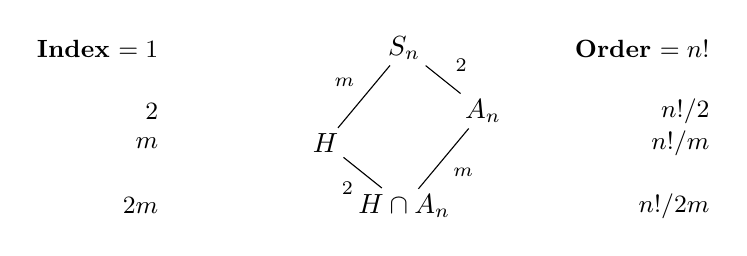
\begin{tikzpicture}[shorten >= -2pt, shorten <= -2pt,scale=1]
      \begin{scope}[shift={(-3,0)}]
     \tikzstyle{every node}=[font=\small]
      \node[anchor=east] at (0,2) {\textbf{Index} $=1$};
      \node[anchor=east] at (0,1.2) {$2$};
      \node[anchor=east] at (0,.8) {$m$};
      \node[anchor=east] at (0,0) {$2m$};
   \end{scope}
   %%
   \begin{scope}[shift={(4,0)}]
     \tikzstyle{every node}=[font=\small]
      \node[anchor=east] at (0,2) {\textbf{Order} $=n!$};
      \node[anchor=east] at (0,1.2) {$n!/2$};
      \node[anchor=east] at (0,.8) {$n!/m$};
      \node[anchor=east] at (0,0) {$n!/2m$};
   \end{scope}
   %%
    \begin{scope}[shift={(0,0)}]
      \node(AB) at (0,2) {$S_n$};
      \node(A) at (-1,.8) {$H$};
      \node(B) at (1,1.2) {$A_n$};
      \node(AcapB) at (0,0) {$H\cap A_n$};
      \path[-] (AB) edge node[above left,pos=.5] {\scriptsize $m$} (A);
      \path[-] (AB) edge node[above right,pos=.6] {\scriptsize $2$} (B);
      \path[-] (AcapB) edge node[below left,pos=.5] {\scriptsize $2$} (A);
      \path[-] (AcapB) edge node[below right,pos=.5] {\scriptsize $m$} (B);
    \end{scope}
  \end{tikzpicture}
  \]
  
  \Pause
  
  \begin{exampleblock}{Proof}
    It suffices to show that $[H:H\cap A_n]=2$, or
    equivalently, that $H/(H\cap A_n)\cong C_2$. \medskip\Pause
    
    Since $H\nleq A_n$, the product $HA_n$ must be strictly larger,
    and so $HA_n=S_n$. \medskip\Pause
    
    By the diamond theorem,
    \[
    H/(H\cap A_n)=HA_n/A_n=S_n/A_n\cong C_2. \tag*{$\hfill\Box$}
    \]
  \end{exampleblock}
  
\end{frame}

%%====================================================================

\begin{frame}{A generalization of the FHT} 
  
  \begin{block}{Theorem (exercise)}
    Every homomorphism $\phi\colon G\to H$ can be \Balert{factored} as
    a quotient and embedding: \vspace{-1mm}
    %%
    %% Commutative diagram: quotient + embedding 
    %%
    \[
    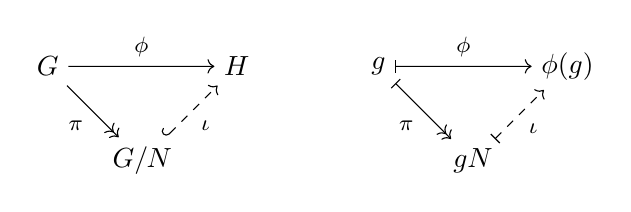
\begin{tikzpicture}[scale=1.2,baseline=(current bounding  box.center)]]
        \begin{scope}[shift={(0,0)}]
          \node (G) at (-1,1) {$G$};
          \node (G/N) at (0,0) {$G/N$};
          \node (H) at (1,1) {$H$};
          \draw[->>] (G) -- (G/N) node[midway,below left]{\footnotesize $\pi$};
          \draw[->] (G) -- (H) node[midway,above]{\footnotesize $\phi$};
          \draw[right hook->,dashed] (G/N) -- (H) node[midway,below right]{\footnotesize $\iota$};
        \end{scope}
        %%
        \begin{scope}[shift={(3.5,0)}]
          \node (G) at (-1,1) {$g$};
          \node (G/N) at (0,0) {$gN$};
          \node (H) at (1,1) {$\phi(g)$};
          \draw[|->>] (G) -- (G/N) node[midway,below left]{\footnotesize $\pi$};
          \draw[|->] (G) -- (H) node[midway,above]{\footnotesize $\phi$};
          \draw[|->,dashed] (G/N) -- (H) node[midway,below right]{\footnotesize $\iota$};
        \end{scope}
    \end{tikzpicture}
    \]
  \end{block}
  
  \vspace{-2mm}
  
  %%
  %% Commutative diagram showing a homomorphism $Q_8\to A_4$ factoring through $V_4$ (lattices)
  %%
  \[
  \begin{tikzpicture}[scale=1.1,shorten >= -2.5pt, shorten <= -2.5pt,scale=.65]
    \tikzstyle{every node}=[font=\small]
    \tikzstyle{E} = [draw, faded];
    \tikzstyle{V} = [faded];
    \tikzstyle{N} = [draw, very thick, eBlue];
    \tikzstyle{H} = [draw, very thick, eRed];
    %%
    %%  G=Q_8
    \begin{scope}[shift={(0,0)}]
      \node[black] (Q8) at (0,3) {$\hspace{-5mm}G\!=\!Q_8$};
      \node[black] (i) at (-1,2) {$\<i\>$};
      \node[black] (j) at (0,2) {$\<j\>$};
      \node[black] (k) at (1,2) {$\<k\>$};
      \node[xBlue] (-1) at (0,1) {$\hspace{-10mm}\Ker(\phi)\!=\!\<-1\>$};
      \node[xBlue] (1) at (0,0) {$\<1\>$};
      \draw (Q8)--(i); 
      \draw (Q8)--(j); 
      \draw (Q8)--(k);
      \draw (-1)--(i); 
      \draw (-1)--(j); 
      \draw (-1)--(k);
      \draw[N] (1)--(-1); 
      \draw [->, thick] (1.75,2) to [bend left=0] node[above] {$\phi$} (7.5,2);
      \draw [->>, thick] (1,1) to [bend left=0] node[below left] {$\pi$} (3.5,-1);
    \end{scope}
    %% Q=V_4
    \begin{scope}[shift={(4.5,-2.5)}]
      \node (Q8) at (0,2) {$\hspace{9mm}G/N\!\cong\!\Image(\phi)$};
      \node (i) at (-1,1) {$\<iN\>$};
      \node (j) at (0,1) {$\<jN\>$};
      \node (k) at (1,1) {$\<kN\>$};
      \node (-1) at (0,0) {$\<N\>$};
      \draw (Q8)--(i); 
      \draw (Q8)--(j); 
      \draw (Q8)--(k);
      \draw (-1)--(i); 
      \draw (-1)--(j); 
      \draw (-1)--(k);
      \draw [right hook->, thick,dashed] (1.5,1.25) to [bend left=0] node[below right] {$\iota$} (3.75,3);
    \end{scope}
    %%
    \begin{scope}[shift={(10,0)},xscale=1.2]
      \node[faded] (A4) at (0,3.25) {$\hspace{4mm}A_4\!=\!H$};
      \node (V4) at (-.65,2) {$\hspace{-8mm}\Image(\phi)\!=\!V_4$};
      \node[V] (C34) at (.25,1.5) {$C_3$};
      \node[V] (C33) at (.65,1.5){$C_3$};
      \node[V] (C32) at (1.05,1.5){$C_3$};
      \node[V] (C31) at (1.45,1.5) {$C_3$};
      \node (C21) at (-.25,1) {$C_2$};
      \node (C22) at (-.65,1) {$C_2$};
      \node (C23) at (-1.05,1) {$C_2$};
      \node (1) at (0,0) {$C_1$};
      \draw[E] (A4)--(V4);
      \draw[E] (A4)--(C31);
      \draw[E] (A4)--(C32);
      \draw[E] (A4)--(C33);
      \draw[E] (A4)--(C34);
      \draw[E] (C31)--(1);
      \draw[E] (C32)--(1);
      \draw[E] (C33)--(1);
      \draw[E] (C34)--(1);
      \draw (V4)--(C21);
      \draw (V4)--(C22);
      \draw (V4)--(C23);
      \draw (C21)--(1);
      \draw (C22)--(1);
      \draw (C23)--(1);
    \end{scope}
    \node at (4.5,1) {\Large $\phi=\iota\circ\pi$};
 \end{tikzpicture}
 \]
 
\end{frame}

%%====================================================================

\begin{frame}{A generalization of the FHT} 

  %%
  %% Commutative diagram showing a homomorphism $Q_8\to A_4$ factoring through $V_4$ (Cayley graphs)
  %%
  \[
  \begin{tikzpicture}[scale=1]
    %%    
    \tikzstyle{every node}=[font=\small]    
    %%
    \begin{scope}[shift={(0,0)}]
      \draw[cosetBlue, fill=cosetBlue] (45:1) circle (.35);
      \draw[cosetBlue, fill=cosetBlue] (135:1) circle (.35);
      \draw[cosetBlue, fill=cosetBlue] (-45:1) circle (.35);
      \draw[cosetBlue, fill=cosetBlue] (-135:1) circle (.35);
      \draw[cosetBlue, fill=cosetBlue] (45:2) circle (.35);
      \draw[cosetBlue, fill=cosetBlue] (135:2) circle (.35);
      \draw[cosetBlue, fill=cosetBlue] (-45:2) circle (.35);
      \draw[cosetBlue, fill=cosetBlue] (-135:2) circle (.35);
      \draw[cosetBlue, fill=cosetBlue,rotate=45] (1,.35) rectangle (2,-.35);
      \draw[cosetBlue, fill=cosetBlue,rotate=135] (1,.35) rectangle (2,-.35);
      \draw[cosetBlue, fill=cosetBlue,rotate=-45] (1,.35) rectangle (2,-.35);
      \draw[cosetBlue, fill=cosetBlue,rotate=-135] (1,.35) rectangle (2,-.35);
      %%
      \node (1) at (135:2) [v] {$1$};
      \node (i) at (45:2) [v] {$i$};
      \node (k) at (-45:2) [v] {$k$};
      \node (j) at (-135:2) [v] {$j$};
      \node (-1) at (135:1) [v] {$-1$};
      \node (-i) at (45:1) [v] {$-i$};
      \node (-k) at (-45:1) [v] {$-k$};
      \node (-j) at (-135:1) [v] {$-j$};
      \node at (-1.8,.95) {\small $\mathbf{N}$};
      \node at (-1.8,-.95) {\small $\mathbf{jN}$};
      \node at (1.8,.95) {\small $\mathbf{iN}$};
      \node at (1.8,-.95) {\small $\mathbf{kN}$};
      %%
      \path[b] (1) to (i);
      \path[b] (i) to (-1);
      \path[b] (-1) to (-i);
      \path[b] (-i) to (1);
      %%
      \path[b] (-j) to (-k);
      \path[b] (-k) to (j);
      \path[b] (j) to (k);
      \path[b] (k) to (-j);
      %%
      \path[r] (-k) to (-i);
      \path[r] (-i) to (k);
      \path[r] (k) to (i);
      \path[r] (i) to (-k);
      %% 
      \path[r] (1) to (j);
      \path[r] (j) to (-1);
      \path[r] (-1) to (-j);
      \path[r] (-j) to (1);
      %%
      \path[gg] (1) to (-1);
      \path[gg] (j) to (-j);
      \path[gg] (i) to (-i);
      \path[gg] (k) to (-k);
      %%
      \node at (0,0) {\normalsize $Q_8$};        
      \draw[->] (1.75,0) -- (5.25,0) node[midway,above]{$\phi$};
      \draw[->>] (0,-1.75) -- (2.25,-4) node[midway,below left]{$\pi$};
    \end{scope}
    %%
    \begin{scope}[shift={(3.5,-4)},scale=.8]
      \tikzstyle{v} = [circle,fill=lightgray,draw,inner sep=0pt, minimum size=7mm]
      \node[v] (e) at (135:1.5) [v] {\small $N$};
      \node[v] (h) at (45:1.5) [v] {\small $iN$};
      \node[v] (v) at (-135:1.5) [v] {\small $jN$};
      \node[v] (b) at (-45:1.5) [v] {\small $kN$};   
      \draw [bb] (e) to (h);
      \draw [bb] (v) to (b);
      \draw [rr] (e) to (v);
      \draw [rr] (h) to (b);
      \node at (0,0) {$\bm{Q_8/N\!\cong\!V_4}$};
      \draw[right hook->,dashed] (1.6,0) -- (4.25,2.1) node[midway,below
        right]{$\iota$};
    \end{scope}
    %%
    %%
    %%
    \begin{scope}[shift={(7.25,0)},scale=.75,bend angle=55]
      \tikzstyle{every node}=[font=\small]
      \tikzstyle{v-light} = [circle, draw, gray, fill=lightgray,inner sep=0pt, 
        minimum size=5.5mm]
      %%
      \begin{scope}[shift={(0:2)}]
        \node at (0,1.75) {\normalsize $\bm{H=A_4}$};
        \node (e) at (-.75,.75) [v] {$e$};
        \node (x) at (.75,.75) [v] {$x$};
        \node (z) at (-.75,-.75) [v] {$z$};
        \node (y) at (.75,-.75) [v] {$y$};
      \end{scope}
      %%
      \begin{scope}[shift={(120:2)}]
        \node[v-light] (a) at (-.75,.75) [v] {$a$};
        \node[v-light] (c) at (.75,.75) [v] {$c$};
        \node[v-light] (d) at (-.75,-.75) [v] {$d$};
        \node[v-light] (b) at (.75,-.75) [v] {$b$};
        \draw [bbFaded] (a) to (c);
        \draw [bbFaded] (d) to (b);
        \draw [rrFaded] (a) to (d);
        \draw [rrFaded] (c) to (b);
      \end{scope}
      %%
      \begin{scope}[shift={(240:2)}]
        \node[v-light] (dd) at (.75,-.75) [v] {$d^2$};
        \node[v-light] (bb) at (.75,.75) [v] {$b^2$};
        \node[v-light] (aa) at (-.75,.75) [v] {$a^2$};
        \node[v-light] (cc) at (-.75,-.75) [v] {$c^2$}; 
        \draw [bbFaded] (aa) to (bb);
        \draw [bbFaded] (cc) to (dd);
        \draw [rrFaded] (aa) to (cc);
        \draw [rrFaded] (bb) to (dd);
      \end{scope}
      %%
      \draw [gFaded] (x) to [bend right=20] (b);
      \draw [gFaded] (e) to [bend right=20] (a);
      \draw [gFaded] (z) to [bend right=7] (c);
      \draw [gFaded] (y) to [bend right=5] (d);
      \draw [gFaded] (a) to [bend right=25] (aa);
      \draw [gFaded] (b) to [bend right=8] (cc);
      \draw [gFaded] (c) to [bend right=22] (dd);
      \draw [gFaded] (d) to [bend right=10] (bb);
      \draw [gFaded] (aa) to [bend right=10] (e);
      \draw [gFaded] (bb) to [bend right=25] (y);
      \draw [gFaded] (cc) to [bend right=25] (x);
      \draw [gFaded] (dd) to [bend right=10] (z);
      \draw [bb] (e) to (x);
      \draw [bb] (z) to (y);
      \draw [rr] (e) to (z);
      \draw [rr] (x) to (y);
      \node at (0:2) {\normalsize $\Image(\phi)$};
    \end{scope}
    \node at (3.5,-1.5) {\Large $\phi=\iota\circ\pi$};
  \end{tikzpicture}
  \]
  
\end{frame}

%%====================================================================

\begin{frame}{A theorem of Hans Zassenhaus} \setbeamercovered{invisible}

  \begin{block}{Butterfly lemma (see book for proof)}
    Let $A,B$ be subgroups of a group, that contain $M\normaleq A$ and
    $N\normaleq B$. Then
    \begin{enumerate}
    \item $(A\cap N)M\normaleq (A\cap B)M$,
    \item $(B\cap M)N\normaleq (A\cap B)N$,
    \item The following quotient groups are isomorphic:
      \[
      \frac{(A\cap B)M}{(A\cap N)M}\cong\frac{(A\cap B)N}{(B\cap M)N}.
      \]
    \end{enumerate}
  \end{block}

  \vspace{-2mm}\pause
  
  \[
  \begin{tikzpicture}[scale=.6]
    \begin{scope}[scale=1,shorten >= -2pt, shorten <= -2pt]
      \tikzstyle{every node}=[font=\footnotesize]
      \node (AM) at (-1.5,0) {$A\cap M$};
      \node (BN) at (1.5,0) {$B\cap N$};
      \node (AMBN) at (0,1.5) {$(A\cap M)(B\cap N)$};
      \node (M) at (-3,1.75) {$M$};
      \node (N) at (3,1.75) {$N$};
      \node (BMN) at (1.5,3) {$(B\cap M)N$};
      \node (ANM) at (-1.5,3) {$(A\cap N)M$};
      \node (AB) at (0,4) {$A\cap B$};
      \node (ABM) at (-1.5,5.25) {$(A\cap B)M$};
      \node (ABN) at (1.5,5.25) {$(A\cap B)N$};
      \node (A) at (-1.5,6.25) {$A$};
      \node (B) at (1.5,6.25) {$B$};
      \draw (AM) to (M); \draw (BN) to (N);
      \draw (AM) to (AMBN); 
      \draw (BN) to (AMBN);
      \draw (ANM) to (AMBN); \draw (BMN) to (AMBN);
      \draw [very thick,eBlue] (AB) to (AMBN);
      \draw (M) to (ANM); \draw (N) to (BMN);
      \draw (ABM) to (AB);
      \draw (ABN) to (AB);
      \draw [very thick,eBlue] (ABM) to (ANM);
      \draw [very thick,eBlue] (ABN) to (BMN);
      \draw (A) -- (ABM); \draw (B) -- (ABN); 
    \end{scope}
    %%
    \begin{scope}[shift={(8,0)},scale=1,shorten >= -2pt, shorten <= -2pt]
      \tikzstyle{every node}=[font=\footnotesize]
      \node (AM) at (-3.5,6.25) {$A\cap M$};
      \node (BN) at (3.5,6.25) {$B\cap N$};
      \node (AMBN) at (0,4.75) {$(A\cap M)(B\cap N)$};
      \node (M) at (-3,4.25) {$M$};
      \node (N) at (3,4.25) {$N$};
      \node (BMN) at (1.5,3.75) {$(B\cap M)N$};
      \node (ANM) at (-1.5,3.75) {$(A\cap N)M$};
      \node (AB) at (0,3) {$A\cap B$};
      \node (ABM) at (-2,1) {$(A\cap B)M$};
      \node (ABN) at (2,1) {$(A\cap B)N$};
      \node (A) at (-3,0) {$A$};
      \node (B) at (3,0) {$B$};
      \draw (AM) to (M); \draw (BN) to (N);
      \draw (AM) to [bend left] (AMBN); 
      \draw (BN) to [bend right] (AMBN);
      \draw (ANM) to (AMBN); \draw (BMN) to (AMBN);
      \draw [very thick,eBlue] (AB) to (AMBN);
      \draw (M) to (ANM); \draw (N) to (BMN);
      \draw (ABM) to [bend right] (AB);
      \draw (ABN) to [bend left] (AB);
      \draw [very thick,eBlue] (ABM) to [bend left] (ANM);
      \draw [very thick,eBlue] (ABN) to [bend right] (BMN);
      \draw (A) -- (ABM); \draw (B) -- (ABN); 
    \end{scope}
  \end{tikzpicture}
  \]
  
\end{frame}


%%====================================================================

\begin{frame}{The quotient $G/Z(G)$ can \emph{never} be a nontrivial cyclic subgroup}
  
  \begin{block}{Lemma (exercise; see images below)}
    If $G/Z(G)$ is cyclic, then $G$ is abelian.
  \end{block}

  \vspace{-4mm}

  %% Shoebox diagram of G/Z(G), and the subgroup lattice of C7xC6.
  \[
  \begin{tikzpicture}[scale=.7]
    %%
    \newcommand\Hh{6.5} % height of 42
    \newcommand\Hg{5.5} % height of 21
    \newcommand\Hf{4.5} % height of 14
    \newcommand\He{3.5} % height of 7
    \newcommand\Hd{2.5} % height of 6
    \newcommand\Hc{1.5} % height of 3
    \newcommand\Hb{1} % height of 2
    \newcommand\Ha{0} % height of 1
    \tikzstyle{every node}=[font=\footnotesize,anchor=south]
    \begin{scope}[shift={(0,0)},scale=1.5,xscale=1.1]
      \node at (2.25,3.25)
            {\normalsize \emph{$\bm{G/Z(G)=\<gZ\>}$, where $Z\!=\!Z(G)$}};
      \draw[thin] (0,0) rectangle (4.5,3);
      \draw[thin,fill=faded] (0,0) rectangle (4.5,.5);
      \draw[thin] (0,2.5) to (4.5,2.5);
      \draw[thin] (0,1.5) to (4.5,1.5);
      \draw[thin] (0,1) to (4.5,1);
      %%
      \node[anchor=west] at (.2,2.77) {$\bullet\;g^{n-1}$};
      \node[anchor=west] at (.85,2.77) {$\bullet\;g^{n-1}\!z_1$};
      \node[anchor=west] at (1.7,2.77) {$\bullet\;g^{n-1}\!z_2$};
      \node[anchor=west] at (2.55,2.77) {$\bullet\;g^{n-1}\!z_3$};
      \node[anchor=west] at (3.35,2.77) {$\cdots$};
      \node[anchor=east] at (4.43,2.77) {\normalsize $\bm{g^{n-1}\!Z}$};
      %%
      \node at (2.25,1.77) {\Large $\bm\vdots$};
      %%
      \node[anchor=west] at (.2,1.27) {$\bullet\;g^2$};
      \node[anchor=west] at (.85,1.27) {$\bullet\;g^2z_1$};
      \node[anchor=west] at (1.7,1.27) {$\bullet\;g^2\!z_2$};
      \node[anchor=west] at (2.55,1.27) {$\bullet\;g^2\!z_3$};
      \node[anchor=west] at (3.35,1.27) {$\cdots$};
      \node[anchor=east] at (4.43,1.27) {\normalsize $\bm{g^2\!Z}$};
      %%
      \node[anchor=west] at (.2,.77) {$\bullet\;g$};
      \node[anchor=west] at (.85,.77) {$\bullet\;gz_1$};
      \node[anchor=west] at (1.7,.77) {$\bullet\;gz_2$};
      \node[anchor=west] at (2.55,.77) {$\bullet\;gz_3$};
      \node[anchor=west] at (3.35,.77) {$\cdots$};
      \node[anchor=east] at (4.43,.77) {\normalsize $\bm{gZ}$};
      %%
      \node[anchor=west] at (.2,.27) {$\bullet\;e$};
      \node[anchor=west] at (.85,.27) {$\bullet\;z_1$};
      \node[anchor=west] at (1.7,.27) {$\bullet\;z_2$};
      \node[anchor=west] at (2.55,.27) {$\bullet\;z_3$};
      \node[anchor=west] at (3.35,.27) {$\cdots$};
      \node[anchor=east] at (4.43,.27) {\normalsize $\bm{Z}$};
      %%
    \end{scope}
    %%
    \begin{scope}[shift={(11.8,-1.25)},scale=1,shorten >= -1pt, shorten <= -1pt,xscale=.7,yscale=1.15]
      \tikzstyle{every node}=[font=\footnotesize]
      \node(G) at (-1.75,\Hh) {\small $C_7\!\rtimes\!C_6$};
      \node(C7-C3) at (-4.25,\Hg) {\small $C_7\!\rtimes\!C_3$};
      \node(D7) at (-1.75,\Hf) {\small $D_7$};
      \node(C7) at (-4.25,\He) {\small $C_7$};
      \node(C3-1) at (-1.25,\Hc) {$C_3$};
      \node(C3-2) at (-.75,\Hc) {$C_3$};
      \node(C3-3) at (-.25,\Hc) {$C_3$};
      \node(C3-4) at (.25,\Hc) {$C_3$};
      \node(C3-5) at (.75,\Hc) {$C_3$};
      \node(C3-6) at (1.25,\Hc) {$C_3$};
      \node(C3-7) at (1.75,\Hc) {$C_3$};
      \node(C6-1) at (3.25,\Hd) {$C_6$};
      \node(C6-2) at (3.75,\Hd) {$C_6$};
      \node(C6-3) at (4.25,\Hd) {$C_6$};
      \node(C6-4) at (4.75,\Hd) {$C_6$};
      \node(C6-5) at (5.25,\Hd) {$C_6$};
      \node(C6-6) at (5.75,\Hd) {$C_6$};
      \node(C6-7) at (6.25,\Hd) {$C_6$};
      \node(C2-1) at (3.25,\Hb) {$C_2$};
      \node(C2-2) at (3.75,\Hb) {$C_2$};
      \node(C2-3) at (4.25,\Hb) {$C_2$};
      \node(C2-4) at (4.75,\Hb) {$C_2$};
      \node(C2-5) at (5.25,\Hb) {$C_2$};
      \node(C2-6) at (5.75,\Hb) {$C_2$};
      \node(C2-7) at (6.25,\Hb) {$C_2$};
      \node(1) at (0,\Ha) {\small $C_1$};
      \draw[faded] (G) to (C7-C3);
      \draw[faded] (G) to (D7);
      \draw[faded] (G) to (C6-1);
      \draw[faded] (G) to (C6-2);
      \draw[faded] (G) to (C6-3);
      \draw[faded] (G) to (C6-4);
      \draw[faded] (G) to (C6-5);
      \draw[faded] (G) to (C6-6);
      \draw[faded] (G) to (C6-7);
      \draw[faded] (D7) to (C7);
      \draw[faded] (D7) to (C2-1);
      \draw[faded] (D7) to (C2-2);
      \draw[faded] (D7) to (C2-3);
      \draw[faded] (D7) to (C2-4);
      \draw[faded] (D7) to (C2-5);
      \draw[faded] (D7) to (C2-6);
      \draw[faded] (D7) to (C2-7);
      \draw[faded] (C7-C3) to (C7);
      \draw[faded] (C7) to (1);
      \draw[faded] (C7-C3) to (C3-1);
      \draw[faded] (C7-C3) to (C3-2);
      \draw[faded] (C7-C3) to (C3-3);
      \draw[faded] (C7-C3) to (C3-4);
      \draw[faded] (C7-C3) to (C3-5);
      \draw[faded] (C7-C3) to (C3-6);
      \draw[faded] (C7-C3) to (C3-7);
      \draw[faded] (C6-1) to (C2-1);
      \draw[faded] (C6-2) to (C2-2);
      \draw[faded] (C6-3) to (C2-3);
      \draw[faded] (C6-4) to (C2-4);
      \draw[faded] (C6-5) to (C2-5);
      \draw[faded] (C6-6) to (C2-6);
      \draw[faded] (C6-7) to (C2-7);
      \draw[faded] (C6-1) to (C3-1);
      \draw[faded] (C6-2) to (C3-2);
      \draw[faded] (C6-3) to (C3-3);
      \draw[faded] (C6-4) to (C3-4);
      \draw[faded] (C6-5) to (C3-5);
      \draw[faded] (C6-6) to (C3-6);
      \draw[faded] (C6-7) to (C3-7);
      \draw[faded] (1) to (C3-1);
      \draw[faded] (1) to (C3-2);
      \draw[faded] (1) to (C3-3);
      \draw[faded] (1) to (C3-4);
      \draw[faded] (1) to (C3-5);
      \draw[faded] (1) to (C3-6);
      \draw[faded] (1) to (C3-7);
      \draw[faded] (1) to (C2-1);
      \draw[faded] (1) to (C2-2);
      \draw[faded] (1) to (C2-3);
      \draw[faded] (1) to (C2-4);
      \draw[faded] (1) to (C2-5);
      \draw[faded] (1) to (C2-6);
      \draw[faded] (1) to (C2-7);
    \end{scope}
    \end{tikzpicture}
%    \caption{Left: If $G/Z(G)$ is cyclic, then arbitrary elements $a,b\in G$ must have the form $a=g^iz_1$ and $b=g^jz_2$ for some $i,j\in\Z$ and $z_1,z_2\in Z(G)$. Right: The center of $G=C_7\!\rtimes\!C_6$ cannot be $C_7\!\rtimes\!C_3$, $D_7$, and $C_7$ because these all have cyclic quotients with $G$.}\label{fig11:F-contraction-lemma}
  \]
  Note that if $G$ is abelian, then $Z(G)=G$.
  
  \end{frame}

%%====================================================================

\begin{frame}{Commutators}
  
  We've seen how to divide $\Z$ by $\<12\>$, thereby ``forcing'' all
  multiples of $12$ to be zero. This is one way to construct the
  integers modulo 12: $\Z_{12}\cong\Z/\<12\>$.
  
  \medskip\Pause
  
  Now, suppose $G$ is nonabelian. We'd like to divide $G$ by its
  ``non-abelian parts,'' making them zero and leaving only ``abelian
  parts'' in the resulting quotient.
  
  \medskip\Pause
  
  A \Alert{commutator} is an element of the form $aba^{-1}b^{-1}$.
  Since $G$ is nonabelian, \emph{there are non-identity commutators:
    $aba^{-1}b^{-1}\neq e$ in $G$}.

  %%
  %% Commutators in the Cayley graph
  %%
  \[
  \begin{tikzpicture}[scale=.6,auto]
  \tikzstyle{v} = [circle, draw, fill=lightgray,inner sep=0pt, 
    minimum size=2.25mm]
    \begin{scope}[shift={(0,0)}]
      \node at (-1.75,0) {$ab=ba$};
      \node (e) at (0,0) [v] {{\tiny $*$}};
      \node (a) at (1,-1) [v] {};
      \node (b) at (1,1) [v] {};
      \node (ab) at (2,0) [v] {};
      \draw [b] (e) to (a);
      \draw [r] (a) to (ab);
      \draw [r] (e) to (b);
      \draw [b] (b) to (ab);
    \end{scope}
    %%
    \begin{scope}[shift={(8,0)}]
      \node at (-1.75,0) {$ab\neq ba$};
      \node (e) at (0,0) [v] {{\tiny $*$}};
      \node (a) at (1,1) [v] {};
      \node (b) at (2.3,1) [v] {};
      \node (c) at (3.3,0) [v] {};
      \node (d) at (2.3,-1) [v] {};
      \draw [r] (e) to (a);
      \draw [b] (a) to (b);
      \draw [r] (c) to (b);
      \draw [b] (d) to (c);
    \end{scope}
  \end{tikzpicture}
  \]
  In this case, the set
  $C:=\{aba^{-1}b^{-1}\mid a,b\in G\}$ contains \emph{more} than the identity.
  
  \smallskip\Pause  
  
  \begin{block}{Definition}
    The \Alert{commutator subgroup} $G'$ of $G$ is
    \[
    G':=\left\<aba^{-1}b^{-1}\mid a,b\in G\right\>.
    \]
  \end{block}

  \smallskip\Pause
  
  The commutator subgroup is normal in $G$, and $G/G'$ is abelian
  (homework).
  
\end{frame}

%%====================================================================

\begin{frame}{The abelianization of a group} 
  
  \begin{block}{Definition}
    The \Alert{abelianization} of $G$ is the quotient group
    $G/G'$.
  \end{block}
  
  \smallskip\Pause
  
  The commutator subgroup $G'$ is the \Balert{smallest normal
    subgroup} $N$ of $G$ such that $G/N$ is abelian. {[Note that $G$
      would be the ``largest'' such subgroup.]}
  
  \medskip\Pause
  
  Equivalently, the quotient $G/G'$ is the {\color{blue}largest
    abelian quotient} of $G$. {[Note that $G/G\cong\<e\>$ would be the
      ``smallest'' such quotient.]}
  
  \smallskip\Pause
  
  \begin{exampleblock}{Universal property of commutator subgroups}
    Suppose $f\colon G\to A$ is a homomorphism to an abelian group
    $A$. \Pause Then there is a unique homomorphism $h\colon G/G'\to
    A$ such that $f=h\circ\pi$: \vspace{-2mm}
    \[
    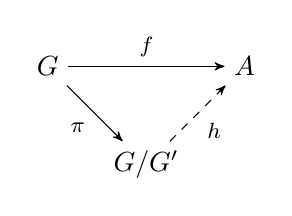
\begin{tikzpicture}[scale=2.5]
    \tikzstyle{e} = [draw, -stealth']
    \begin{scope}[shift={(0,0)}]
        \node (G) at (0,0) {$G$};
        \node (A) at (1,0) {$A$};
        \node (G/G') at (.5,-.5) {$G/G'$};
        \draw [e] (G) -- (A) node[midway,above]{\footnotesize $f$};
        \draw [e] (G) -- (G/G') node[midway,below left]{\footnotesize $\pi$};
        \draw [e,dashed] (G/G') -- (A) node[midway,below right]{\footnotesize $h$};
      \end{scope}
    \end{tikzpicture}
    \]
    We say that $f$ ``factors through'' the
    abelianization, $G/G'$.
  \end{exampleblock}
  
\end{frame}

%%====================================================================

\begin{frame}{Some examples of abelianizations} \smallskip

  By the isormophism theorems, we can usually identitfy the commutator
  subgroup $G$ and abelianation by inspection, from the subgroup lattice.

  \vspace{-5mm}

  %%
  %% Commutator subgroups in subgroup lattices
  %%
  \[
  \begin{tikzpicture}[node distance=1cm,shorten >= -2pt, shorten <= -2pt,
      scale=.5]
    \begin{scope}[shift={(-2,-8)},scale=1.75] %% D_4 lattice
      %\tikzstyle{every node}=[font=\small]
      \node (D4) at (0,4) {$D_4$};
      \node (r2-f) at (-1.25,3) {$\<r^2,f\>$};
      \node (r) at (0,3) {$\<r\>$};
      \node (r2-rf) at (1.25,3) {$\<r^2,rf\>$};
      %%
      \node (f) at (-2.5,2) {$\color{faded}\<f\>$};
      \node (r2f) at (-1.25,2) {$\color{faded}\<r^2f\>$};
      \node (r2) at (0,2) {$\<r^2\>$};
      \node (r3f) at (1.25,2) {$\color{faded}\<r^3f\>$};
      \node (rf) at (2.5,2) {$\color{faded}\<rf\>$};
      %%
      \node (1) at (0,1) {$\color{faded}\<1\>$};
      %%
      \draw (D4) to (r2-f); \draw (D4) to (r); \draw (D4) to (r2-rf);
      \draw[faded] (r2-f) to (f); \draw[faded] (r2-f) to (r2f); 
      \draw (r2-f) to (r2);
      \draw[faded] (r2-rf) to (rf); \draw[faded] (r2-rf) to (r3f); 
      \draw (r2-rf) to (r2); \draw (r2) to (r); 
      \draw[faded] (r2) to (1); \draw[faded] (f) to (1);
      \draw[faded] (r2f) to (1); \draw[faded] (r3f) to (1); 
      \draw (rf)[faded] to (1);
    \end{scope}
    %%
    \begin{scope}[shift={(10.5,1.5)},scale=1,shorten >= -2pt, shorten <= -2pt]
      %\tikzstyle{every node}=[font=\small]
      \node(G) at (0,6) {$\Dic_6$};
      \node(b) at (-1.5,4.5) {$\<r\>$};
      \node(aa) at (0,1.5) {$\color{faded}\<r^3\>$};
      \node(bb) at (-2,2.25) {$\<r^2\>$};
      \node(a) at (.5,24/7) {$\color{faded}\<s\>$};
      \node(ab) at (1.75,24/7) {$\color{faded}\<rs\>$};
      \node(ba) at (3,24/7) {$\color{faded}\<r^2\!s\>$};
      \node(1) at (0,0) {$\color{faded}\left\<1\right\>$};
      \draw[faded] (1) to (aa); 
      \draw[faded] (1) to (bb);
      \draw[faded] (b) to (aa);
      \draw (b) to (bb);
      \draw[faded] (aa) to (a);
      \draw[faded] (aa) to (ab);
      \draw[faded] (aa) to (ba);
      \draw[faded] (G) to (a);
      \draw[faded] (G) to (ab);
      \draw[faded] (G) to (ba);
      \draw (G) to (b);   
    \end{scope}
    %%
    \begin{scope}[shift={(0,0)},scale=1.1]
      \tikzstyle{every node}=[font=\small]
      \node(A4) at (0,6) {\small $A_4$};
      \node(V4) at (2.25,4) {$\<(12)(34),(13)(24)\>$};
      \node(C34) at (-.75,3) {$\color{faded}\<(234)\>$};
      \node(C33) at (-2.25,3){$\color{faded}\<(134)\>$};
      \node(C32) at (-3.75,3){$\color{faded}\<(124)\>$};
      \node(C31) at (-5.25,3) {$\color{faded}\<(123)\>$};
      \node(C21) at (.75,2) {\footnotesize $\color{faded}\<(12)(34))\>$};
      \node(C22) at (2.75,2) {\footnotesize $\color{faded}\<(13)(24)\>$};
      \node(C23) at (4.75,2) {\footnotesize $\color{faded}\<(14)(23))\>$};
      \node(1) at (0,0) {$\color{faded}\left\<e\right\>$};
      \draw (A4)--(V4);
      \draw[faded] (A4)--(C31);
      \draw[faded] (A4)--(C32);
      \draw[faded] (A4)--(C33);
      \draw[faded] (A4)--(C34);
      \draw[faded] (C31)--(1);
      \draw[faded] (C32)--(1);
      \draw[faded] (C33)--(1);
      \draw[faded] (C34)--(1);
      \draw[faded] (V4)--(C21);
      \draw[faded] (V4)--(C22);
      \draw[faded] (V4)--(C23);
      \draw[faded] (C21)--(1);
      \draw[faded] (C22)--(1);
      \draw[faded] (C23)--(1);
    \end{scope}
    %%
    \begin{scope}[shift={(9,-6.5)},scale=1.15]
      %\tikzstyle{every node}=[font=\small]
      \node(G) at (3.5,6) {$\SA_8$};
      \node(rs) at (3.5,4.5) {$\<rs\>$};
      \node(r2-s) at (1.75,4.5) {$\<r^2,s\>$};
      \node(r) at (5.25,4.5) {$\<r\>$};
      \node(r4-s) at (0,3) {$\<r^4,s\>$};
      \node(r2s) at (1.75,3) {$\<r^2s\>$};
      \node(r2) at (3.5,3) {$\<r^2\>$};
      \node(s) at (-1.75,1.5) {\color{faded}$\<s\>$};
      \node(r4s) at (0,1.5) {\color{faded}$\<r^4s\>$};
      \node(r4) at (1.75,1.5) {$\<r^4\>$};
      \node(1) at (0,0) {\color{faded}$\<1\>$};
      \draw[faded] (1) -- (s);
      \draw[faded] (1) -- (r4s);
      \draw[faded] (1) -- (r4);
      \draw[faded] (s) -- (r4-s);
      \draw[faded] (r4s) -- (r4-s);
      \draw (r4) -- (r4-s);
      \draw (r4) -- (r2s);
      \draw (r4) -- (r2);
      \draw (r4-s) -- (r2-s);
      \draw (r2s) -- (r2-s);
      \draw (r2) -- (r2-s);
      \draw (r2) -- (r);
      \draw (r2) -- (rs);
      \draw (r2-s) -- (G);
      \draw (r) -- (G);
      \draw (rs) -- (G);
    \end{scope}
  \end{tikzpicture}
  \]
  
\end{frame}

%%====================================================================

\begin{frame}{Automorphisms} %\Pause
  
  We have already seen automorphisms of cyclic groups:
  ``\emph{structure-preserving rewirings}.'' \medskip\Pause
  
  For a general group $G$, an \Alert{automorphism} is a isomorphism
  $\phi\colon G\to G$. \medskip\Pause
  
  The set of automorphisms of $G$ defines the \Balert{automorphism
    group} of $G$, denoted $\Aut(G)$. \medskip\Pause
  
  \begin{block}{Proposition}
    The automorphism group of $\Z_n$ is $\Aut(\Z_n)=\big\{\sigma_a\mid
    a\in U_n\big\}\cong U_n$, where 
    \[
    \sigma_a\colon\Z_n\longto\Z_n\,,\qquad\sigma_a(1)=a\,.
    \]
  \end{block}
  
  \vspace{-4mm}

  %%
  %% Cayley table: U_7 and Aut(C_7)
  %%
  \[
  \begin{tikzpicture}[scale=.55]
    %%    
  \colorlet{color-1}{tYellow}
  \colorlet{color-2}{tRed}
  \colorlet{color-3}{tOrange}
  \colorlet{color-4}{tBlue}
  \colorlet{color-5}{tGreen}
  \colorlet{color-6}{tPurple}
  \tikzstyle{v} = [circle, draw, fill=lightgray,inner sep=0pt,
    minimum size=1.75mm]
  \tikzstyle{r-thin} = [draw, thick, eRed,-stealth]  
    \begin{scope}[shift={(18,6.5)},scale=.9]
      \tikzstyle{every node}=[font=\tiny]
      \node (1) at (0:1) [v] {$1$};
      \node (r) at (51.45:1) [v] {};
      \node (r2) at (102.9:1) [v] {};
      \node (r3) at (154.3:1) [v] {};
      \node (r4) at (205.7:1) [v] {};
      \node (r5) at (257.1:1) [v] {};
      \node (r6) at (308.6:1) [v] {};
      \draw [r-thin] (1) to (r); \draw [r-thin] (r) to (r2); 
      \draw [r-thin] (r2) to (r3); \draw [r-thin] (r3) to (r4);
      \draw [r-thin] (r4) to (r5); \draw [r-thin] (r5) to (r6); 
      \draw [r-thin] (r6) to (1);
      \node at (0,0) {\small $\sigma_1$};
    \end{scope}
    %%
    \begin{scope}[shift={(16,4)},scale=.9]
      \tikzstyle{every node}=[font=\tiny]
      \node (1) at (0:1) [v] {$1$};
      \node (r) at (51.45:1) [v] {};
      \node (r2) at (102.9:1) [v] {};
      \node (r3) at (154.3:1) [v] {};
      \node (r4) at (205.7:1) [v] {};
      \node (r5) at (257.1:1) [v] {};
      \node (r6) at (308.6:1) [v] {};
      \draw [r-thin] (1) to (r2); \draw [r-thin] (r2) to (r4); 
      \draw [r-thin] (r4) to (r6); \draw [r-thin] (r6) to (r);
      \draw [r-thin] (r) to (r3); \draw [r-thin] (r3) to (r5); 
      \draw [r-thin] (r5) to (1);
      \node at (0,0) {\small $\sigma_2$};
    \end{scope}
    %%
    \begin{scope}[shift={(20,4)},scale=.9]
      \tikzstyle{every node}=[font=\tiny]
      \node (1) at (0:1) [v] {$1$};
      \node (r) at (51.45:1) [v] {};
      \node (r2) at (102.9:1) [v] {};
      \node (r3) at (154.3:1) [v] {};
      \node (r4) at (205.7:1) [v] {};
      \node (r5) at (257.1:1) [v] {};
      \node (r6) at (308.6:1) [v] {};
      \draw [r-thin] (1) to (r3); \draw [r-thin] (r3) to (r6); 
      \draw [r-thin] (r6) to (r2); \draw [r-thin] (r2) to (r5);
      \draw [r-thin] (r5) to (r); \draw [r-thin] (r) to (r4); 
      \draw [r-thin] (r4) to (1);
      \node at (0,0) {\footnotesize $\sigma_{\!3}$};
    \end{scope}    
    %%
    \begin{scope}[shift={(18,1.5)},scale=.9]  
      \tikzstyle{every node}=[font=\tiny]
      \node (1) at (0:1) [v] {$1$};
      \node (r) at (51.45:1) [v] {};
      \node (r2) at (102.9:1) [v] {};
      \node (r3) at (154.3:1) [v] {};
      \node (r4) at (205.7:1) [v] {};
      \node (r5) at (257.1:1) [v] {};
      \node (r6) at (308.6:1) [v] {};
      \draw [r-thin] (1) to (r6); \draw [r-thin] (r6) to (r5); 
      \draw [r-thin] (r5) to (r4); \draw [r-thin] (r4) to (r3);
      \draw [r-thin] (r3) to (r2); \draw [r-thin] (r2) to (r); 
      \draw [r-thin] (r) to (1);
      \node at (0,0) {\small $\sigma_6$};
    \end{scope}
    %%
    \tikzstyle{every node}=[font=\small]
    \begin{scope}[scale=0.85,shift={(0,0)}]
      \node at (4,8.7) {\normalsize $\mathbf{U_7=\<3\>\cong C_6}$};
      \path[fill=color-1] (-0.1,6) rectangle ++(1,1);
      \path[fill=color-2] (-0.1,5) rectangle ++(1,1);
      \path[fill=color-3] (-0.1,4) rectangle ++(1,1);
      \path[fill=color-4] (-0.1,3) rectangle ++(1,1);
      \path[fill=color-5] (-0.1,2) rectangle ++(1,1);
      \path[fill=color-6] (-0.1,1) rectangle ++(1,1);
      %%
      \path[fill=color-1] (1,7.1) rectangle ++(1,1);
      \path[fill=color-2] (2,7.1) rectangle ++(1,1);
      \path[fill=color-3] (3,7.1) rectangle ++(1,1);
      \path[fill=color-4] (4,7.1) rectangle ++(1,1);
      \path[fill=color-5] (5,7.1) rectangle ++(1,1);
      \path[fill=color-6] (6,7.1) rectangle ++(1,1);
      %%
      \path[fill=color-1] (1,6) rectangle ++(1,1);
      \path[fill=color-2] (1,5) rectangle ++(1,1);
      \path[fill=color-3] (1,4) rectangle ++(1,1);
      \path[fill=color-4] (1,3) rectangle ++(1,1);
      \path[fill=color-5] (1,2) rectangle ++(1,1);
      \path[fill=color-6] (1,1) rectangle ++(1,1);
      %%
      \path[fill=color-2] (2,6) rectangle ++(1,1);
      \path[fill=color-4] (2,5) rectangle ++(1,1);
      \path[fill=color-6] (2,4) rectangle ++(1,1);
      \path[fill=color-1] (2,3) rectangle ++(1,1);
      \path[fill=color-3] (2,2) rectangle ++(1,1);
      \path[fill=color-5] (2,1) rectangle ++(1,1);
      %%
      \path[fill=color-3] (3,6) rectangle ++(1,1);
      \path[fill=color-6] (3,5) rectangle ++(1,1);
      \path[fill=color-2] (3,4) rectangle ++(1,1);
      \path[fill=color-5] (3,3) rectangle ++(1,1);
      \path[fill=color-1] (3,2) rectangle ++(1,1);
      \path[fill=color-4] (3,1) rectangle ++(1,1);
      %%
      \path[fill=color-4] (4,6) rectangle ++(1,1);
      \path[fill=color-1] (4,5) rectangle ++(1,1);
      \path[fill=color-5] (4,4) rectangle ++(1,1);
      \path[fill=color-2] (4,3) rectangle ++(1,1);
      \path[fill=color-6] (4,2) rectangle ++(1,1);
      \path[fill=color-3] (4,1) rectangle ++(1,1);
      %%
      \path[fill=color-5] (5,6) rectangle ++(1,1);
      \path[fill=color-3] (5,5) rectangle ++(1,1);
      \path[fill=color-1] (5,4) rectangle ++(1,1);
      \path[fill=color-6] (5,3) rectangle ++(1,1);
      \path[fill=color-4] (5,2) rectangle ++(1,1);
      \path[fill=color-2] (5,1) rectangle ++(1,1);
      %%
      \path[fill=color-6] (6,6) rectangle ++(1,1);
      \path[fill=color-5] (6,5) rectangle ++(1,1);
      \path[fill=color-4] (6,4) rectangle ++(1,1);
      \path[fill=color-3] (6,3) rectangle ++(1,1);
      \path[fill=color-2] (6,2) rectangle ++(1,1);
      \path[fill=color-1] (6,1) rectangle ++(1,1);
      %%
      \foreach \i in {1,...,7} {
        \draw [very thin] (\i,1) -- (\i,7); 
        \draw [very thin] (\i,7+.1) -- (\i,7+1.1); 
        \draw [very thin] (1,\i) -- (7,\i); 
        \draw [very thin] (-0.1,\i) -- (.9,\i); 
      } 
      \draw [very thin] (1,7+.1) rectangle (7,7+1.1);
      \draw [very thin] (-0.1,1) rectangle (.9,7);
      \node at (0.4,6.5) {$1$};
      \node at (0.4,5.5) {$2$};
      \node at (0.4,4.5) {$3$};
      \node at (0.4,3.5) {$4$};
      \node at (0.4,2.5) {$5$};
      \node at (0.4,1.5) {$6$};
      %%
      \node at (1.5,7.6) {$1$};
      \node at (2.5,7.6) {$2$};
      \node at (3.5,7.6) {$3$};
      \node at (4.5,7.6) {$4$};
      \node at (5.5,7.6) {$5$};
      \node at (6.5,7.6) {$6$}; %
      %%
      \node at (1.5,6.5) {$1$};
      \node at (1.5,5.5) {$2$};
      \node at (1.5,4.5) {$3$};
      \node at (1.5,3.5) {$4$};
      \node at (1.5,2.5) {$5$};
      \node at (1.5,1.5) {$6$};
      %%
      \node at (2.5,6.5) {$2$};
      \node at (2.5,5.5) {$4$};
      \node at (2.5,4.5) {$6$};
      \node at (2.5,3.5) {$1$};
      \node at (2.5,2.5) {$3$};
      \node at (2.5,1.5) {$5$};
      %%
      \node at (3.5,6.5) {$3$};
      \node at (3.5,5.5) {$6$};
      \node at (3.5,4.5) {$2$};
      \node at (3.5,3.5) {$5$};
      \node at (3.5,2.5) {$1$};
      \node at (3.5,1.5) {$4$};
      %%
      \node at (4.5,6.5) {$4$};
      \node at (4.5,5.5) {$1$};
      \node at (4.5,4.5) {$5$};
      \node at (4.5,3.5) {$2$};
      \node at (4.5,2.5) {$6$};
      \node at (4.5,1.5) {$3$};
      %%
      \node at (5.5,6.5) {$5$};
      \node at (5.5,5.5) {$3$};
      \node at (5.5,4.5) {$1$};
      \node at (5.5,3.5) {$6$};
      \node at (5.5,2.5) {$4$};
      \node at (5.5,1.5) {$2$};
      %%
      \node at (6.5,6.5) {$6$};
      \node at (6.5,5.5) {$5$};
      \node at (6.5,4.5) {$4$};
      \node at (6.5,3.5) {$3$};
      \node at (6.5,2.5) {$2$};
      \node at (6.5,1.5) {$1$};
    \end{scope}
    %%%%
    %%%%%=============================================================
    %%%%
    \begin{scope}[scale=0.85,shift={(9.5,0)}]
      \node at (4,8.7) {\normalsize
        $\mathbf{\Aut(C_7)}=\<\sigma_3\>\cong\mathbf{U_7}$};
      \path[fill=color-1] (-0.1,6) rectangle ++(1,1);
      \path[fill=color-2] (-0.1,5) rectangle ++(1,1);
      \path[fill=color-3] (-0.1,4) rectangle ++(1,1);
      \path[fill=color-4] (-0.1,3) rectangle ++(1,1);
      \path[fill=color-5] (-0.1,2) rectangle ++(1,1);
      \path[fill=color-6] (-0.1,1) rectangle ++(1,1);
      %%
      \path[fill=color-1] (1,7.1) rectangle ++(1,1);
      \path[fill=color-2] (2,7.1) rectangle ++(1,1);
      \path[fill=color-3] (3,7.1) rectangle ++(1,1);
      \path[fill=color-4] (4,7.1) rectangle ++(1,1);
      \path[fill=color-5] (5,7.1) rectangle ++(1,1);
      \path[fill=color-6] (6,7.1) rectangle ++(1,1);
      %%
      \path[fill=color-1] (1,6) rectangle ++(1,1);
      \path[fill=color-2] (1,5) rectangle ++(1,1);
      \path[fill=color-3] (1,4) rectangle ++(1,1);
      \path[fill=color-4] (1,3) rectangle ++(1,1);
      \path[fill=color-5] (1,2) rectangle ++(1,1);
      \path[fill=color-6] (1,1) rectangle ++(1,1);
      %%
      \path[fill=color-2] (2,6) rectangle ++(1,1);
      \path[fill=color-4] (2,5) rectangle ++(1,1);
      \path[fill=color-6] (2,4) rectangle ++(1,1);
      \path[fill=color-1] (2,3) rectangle ++(1,1);
      \path[fill=color-3] (2,2) rectangle ++(1,1);
      \path[fill=color-5] (2,1) rectangle ++(1,1);
      %%
      \path[fill=color-3] (3,6) rectangle ++(1,1);
      \path[fill=color-6] (3,5) rectangle ++(1,1);
      \path[fill=color-2] (3,4) rectangle ++(1,1);
      \path[fill=color-5] (3,3) rectangle ++(1,1);
      \path[fill=color-1] (3,2) rectangle ++(1,1);
      \path[fill=color-4] (3,1) rectangle ++(1,1);
      %%
      \path[fill=color-4] (4,6) rectangle ++(1,1);
      \path[fill=color-1] (4,5) rectangle ++(1,1);
      \path[fill=color-5] (4,4) rectangle ++(1,1);
      \path[fill=color-2] (4,3) rectangle ++(1,1);
      \path[fill=color-6] (4,2) rectangle ++(1,1);
      \path[fill=color-3] (4,1) rectangle ++(1,1);
      %%
      \path[fill=color-5] (5,6) rectangle ++(1,1);
      \path[fill=color-3] (5,5) rectangle ++(1,1);
      \path[fill=color-1] (5,4) rectangle ++(1,1);
      \path[fill=color-6] (5,3) rectangle ++(1,1);
      \path[fill=color-4] (5,2) rectangle ++(1,1);
      \path[fill=color-2] (5,1) rectangle ++(1,1);
      %%
      \path[fill=color-6] (6,6) rectangle ++(1,1);
      \path[fill=color-5] (6,5) rectangle ++(1,1);
      \path[fill=color-4] (6,4) rectangle ++(1,1);
      \path[fill=color-3] (6,3) rectangle ++(1,1);
      \path[fill=color-2] (6,2) rectangle ++(1,1);
      \path[fill=color-1] (6,1) rectangle ++(1,1);
      %%
      \foreach \i in {1,...,7} {
        \draw [very thin] (\i,1) -- (\i,7); 
        \draw [very thin] (\i,7+.1) -- (\i,7+1.1); 
        \draw [very thin] (1,\i) -- (7,\i); 
        \draw [very thin] (-0.1,\i) -- (.9,\i); 
      } 
      \draw [very thin] (1,7+.1) rectangle (7,7+1.1);
      \draw [very thin] (-0.1,1) rectangle (.9,7);
      \node at (0.4,6.5) {$\sigma_1$};
      \node at (0.4,5.5) {$\sigma_2$};
      \node at (0.4,4.5) {$\sigma_3$};
      \node at (0.4,3.5) {$\sigma_4$};
      \node at (0.4,2.5) {$\sigma_5$};
      \node at (0.4,1.5) {$\sigma_6$};
      %%
      \node at (1.5,7.6) {$\sigma_1$};
      \node at (2.5,7.6) {$\sigma_2$};
      \node at (3.5,7.6) {$\sigma_3$};
      \node at (4.5,7.6) {$\sigma_4$};
      \node at (5.5,7.6) {$\sigma_5$};
      \node at (6.5,7.6) {$\sigma_6$};
      %%
      \node at (1.5,6.5) {$\sigma_1$};
      \node at (1.5,5.5) {$\sigma_2$};
      \node at (1.5,4.5) {$\sigma_3$};
      \node at (1.5,3.5) {$\sigma_4$};
      \node at (1.5,2.5) {$\sigma_5$};
      \node at (1.5,1.5) {$\sigma_6$};
      %%
      \node at (2.5,6.5) {$\sigma_2$};
      \node at (2.5,5.5) {$\sigma_4$};
      \node at (2.5,4.5) {$\sigma_6$};
      \node at (2.5,3.5) {$\sigma_1$};
      \node at (2.5,2.5) {$\sigma_3$};
      \node at (2.5,1.5) {$\sigma_5$};
      %%
      \node at (3.5,6.5) {$\sigma_3$};
      \node at (3.5,5.5) {$\sigma_6$};
      \node at (3.5,4.5) {$\sigma_2$};
      \node at (3.5,3.5) {$\sigma_5$};
      \node at (3.5,2.5) {$\sigma_1$};
      \node at (3.5,1.5) {$\sigma_4$};
      %%
      \node at (4.5,6.5) {$\sigma_4$};
      \node at (4.5,5.5) {$\sigma_1$};
      \node at (4.5,4.5) {$\sigma_5$};
      \node at (4.5,3.5) {$\sigma_2$};
      \node at (4.5,2.5) {$\sigma_6$};
      \node at (4.5,1.5) {$\sigma_3$};
      %%
      \node at (5.5,6.5) {$\sigma_5$};
      \node at (5.5,5.5) {$\sigma_3$};
      \node at (5.5,4.5) {$\sigma_1$};
      \node at (5.5,3.5) {$\sigma_6$};
      \node at (5.5,2.5) {$\sigma_4$};
      \node at (5.5,1.5) {$\sigma_2$};
      %%
      \node at (6.5,6.5) {$\sigma_6$};
      \node at (6.5,5.5) {$\sigma_5$};
      \node at (6.5,4.5) {$\sigma_4$};
      \node at (6.5,3.5) {$\sigma_3$};
      \node at (6.5,2.5) {$\sigma_2$};
      \node at (6.5,1.5) {$\sigma_1$};
    \end{scope}
  \end{tikzpicture}
  \]

\end{frame}

%%====================================================================

\begin{frame}{An example: the automorphism group of $C_7$} 

  %%
  %% Cayley graph of Aut(C_7)
  %%
  \[
  \hspace*{-4mm}
  \begin{tikzpicture}[scale=.96,baseline=-.5ex]
  \tikzstyle{v} = [circle, draw, fill=lightgray,inner sep=0pt,
    minimum size=3.5mm]
  \tikzstyle{v-y} = [circle, draw, fill=vYellow,inner sep=0pt, 
    minimum size=3.5mm]
  \tikzstyle{r-thin} = [draw, thick, eRed,-stealth]
    %%
    \node at (0,0) {\Large $\Aut(C_7)\cong U_7=\<3\>$};
    \tikzstyle{every node}=[font=\footnotesize]
    \draw [p] (18:3.5) to [bend right=12] (42:3.5);
    \draw [p] (78:3.5) to [bend right=12] (102:3.5);
    \draw [p] (138:3.5) to [bend right=12] (162:3.5);
    \draw [p] (198:3.5) to [bend right=12] (222:3.5);
    \draw [p] (258:3.5) to [bend right=12] (282:3.5);
    \draw [p] (318:3.5) to [bend right=12] (342:3.5);
    %%
    \begin{scope}[shift={(0:3)},scale=.85]
      \node (1) at (0:1) [v-y] {$1$};
      \node (r) at (51.45:1) [v-y] {$r$};
      \node (r2) at (102.9:1) [v] {$r^2$};
      \node (r3) at (154.3:1) [v] {$r^3$};
      \node (r4) at (205.7:1) [v] {$r^4$};
      \node (r5) at (257.1:1) [v] {$r^5$};
      \node (r6) at (308.6:1) [v] {$r^6$};
      \draw [r-thin] (1) to (r); \draw [r-thin] (r) to (r2);
      \draw [r-thin] (r2) to (r3); \draw [r-thin] (r3) to (r4);
      \draw [r-thin] (r4) to (r5); \draw [r-thin] (r5) to (r6);
      \draw [r-thin] (r6) to (1);
      \node at (0,0) {\Large Id=$\sigma_1$};
    \end{scope}
    %%
    \begin{scope}[shift={(60:3)},scale=.85]
      \node at (2.5,.3) {\normalsize ``\emph{tripling map}'' $\sigma_3$};
      \node at (2.5,-.3) {\normalsize$U_7=\<3\>$};
      \node (1) at (0:1) [v-y] {$1$};
      \node (r) at (51.45:1) [v] {$r$};
      \node (r2) at (102.9:1) [v] {$r^2$};
      \node (r3) at (154.3:1) [v-y] {$r^3$};
      \node (r4) at (205.7:1) [v] {$r^4$};
      \node (r5) at (257.1:1) [v] {$r^5$};
      \node (r6) at (308.6:1) [v] {$r^6$};
      \draw [r-thin] (1) to (r3); \draw [r-thin] (r3) to (r6);
      \draw [r-thin] (r6) to (r2); \draw [r-thin] (r2) to (r5);
      \draw [r-thin] (r5) to (r); \draw [r-thin] (r) to (r4);
      \draw [r-thin] (r4) to (1);
      \node at (0,0) {\Large $\phi$};
    \end{scope}
    %%
    \begin{scope}[shift={(120:3)},scale=.85]
      \node at (-2.8,.3) {\normalsize ``\emph{doubling map}'' $\sigma_2$};
      \node at (-2.8,-.3) {\normalsize $3^2\equiv 2\!\pmod{7}$};
      \node (1) at (0:1) [v-y] {$1$};
      \node (r) at (51.45:1) [v] {$r$};
      \node (r2) at (102.9:1) [v-y] {$r^2$};
      \node (r3) at (154.3:1) [v] {$r^3$};
      \node (r4) at (205.7:1) [v] {$r^4$};
      \node (r5) at (257.1:1) [v] {$r^5$};
      \node (r6) at (308.6:1) [v] {$r^6$};
      \draw [r-thin] (1) to (r2); \draw [r-thin] (r2) to (r4);
      \draw [r-thin] (r4) to (r6); \draw [r-thin] (r6) to (r);
      \draw [r-thin] (r) to (r3); \draw [r-thin] (r3) to (r5);
      \draw [r-thin] (r5) to (1);
      \node at (0,0) {\Large $\phi^2$};
    \end{scope}
    %%
    \begin{scope}[shift={(180:3)},scale=.85]
      \node at (-2.8,.3) {\normalsize ``\emph{sextupling map}'' $\sigma_6$};
      \node at (-2.8,-.3) {\normalsize $3^3\equiv 6\!\pmod{7}$};
      \node (1) at (0:1) [v-y] {$1$};
      \node (r) at (51.45:1) [v] {$r$};
      \node (r2) at (102.9:1) [v] {$r^2$};
      \node (r3) at (154.3:1) [v] {$r^3$};
      \node (r4) at (205.7:1) [v] {$r^4$};
      \node (r5) at (257.1:1) [v] {$r^5$};
      \node (r6) at (308.6:1) [v-y] {$r^6$};
      \draw [r-thin] (1) to (r6); \draw [r-thin] (r6) to (r5);
      \draw [r-thin] (r5) to (r4); \draw [r-thin] (r4) to (r3);
      \draw [r-thin] (r3) to (r2); \draw [r-thin] (r2) to (r);
      \draw [r-thin] (r) to (1);      
      \node at (0,0) {\Large $\phi^3$};
    \end{scope}
    %%
    \begin{scope}[shift={(240:3)},scale=.85]
      \node at (-3.2,.3) {\normalsize ``\emph{quadrupling map}'' $\sigma_4$};
      \node at (-3,-.3) {\normalsize $3^4\equiv 4\!\pmod{7}$};
      \node (1) at (0:1) [v-y] {$1$};
      \node (r) at (51.45:1) [v] {$r$};
      \node (r2) at (102.9:1) [v] {$r^2$};
      \node (r3) at (154.3:1) [v] {$r^3$};
      \node (r4) at (205.7:1) [v-y] {$r^4$};
      \node (r5) at (257.1:1) [v] {$r^5$};
      \node (r6) at (308.6:1) [v] {$r^6$};
      \draw [r-thin] (1) to (r4); \draw [r-thin] (r4) to (r);
      \draw [r-thin] (r) to (r5); \draw [r-thin] (r5) to (r2);
      \draw [r-thin] (r2) to (r6); \draw [r-thin] (r6) to (r3);
      \draw [r-thin] (r3) to (1);      
      \node at (0,0) {\normalsize $\phi^4$};
    \end{scope}
    %%
    \begin{scope}[shift={(300:3)},scale=.85]
      \node at (3.2,.3) {\normalsize ``\emph{quintupling map}'' $\sigma_5$};
      \node at (3.2,-.3) {\normalsize $3^5\equiv 5\!\pmod{7}$};      
      \node (1) at (0:1) [v-y] {$1$};
      \node (r) at (51.45:1) [v] {$r$};
      \node (r2) at (102.9:1) [v] {$r^2$};
      \node (r3) at (154.3:1) [v] {$r^3$};
      \node (r4) at (205.7:1) [v] {$r^4$};
      \node (r5) at (257.1:1) [v-y] {$r^5$};
      \node (r6) at (308.6:1) [v] {$r^6$};
      \draw [r-thin] (1) to (r5); \draw [r-thin] (r5) to (r3);
      \draw [r-thin] (r3) to (r);
      \draw [r-thin] (r) to (r6); \draw [r-thin] (r6) to (r4);
      \draw [r-thin] (r4) to (r2);
      \draw [r-thin] (r2) to (1);      
      \node at (0,0) {\Large $\phi^5$};
    \end{scope}
  \end{tikzpicture}
  \]
  
\end{frame}

%%====================================================================

\begin{frame}{Automorphisms of noncyclic groups}
    
  An automorphism is determined by where it sends the generators.
  
  \begin{exampleblock}{Examples} 
    \begin{enumerate}
    \item An automorphism $\phi$ of $V_4=\<h,v\>$ is determined by the
      image of $h$ and $v$. \medskip\Pause
      
      There are $3$ choices for $\phi(h)$, then $2$ choices for
      $\phi(v)$, thus $|\Aut(V_4)|=6$. \medskip\Pause
      
      Every permutation of $\{h,v,r\}$ is an automorphism, and so
      $\Aut(V_4)\cong S_3$. \medskip\pause
      
    \item Every $\phi\in\Aut(D_3)$ is determined by $\phi(r)$ and
      $\phi(f)$. \medskip\Pause
      
      Since automorphisms preserve order, if $\phi\in\Aut(D_3)$, then 
      \[
      \phi(1)=1\,,\qquad \phi(r)=\underbrace{\text{$r$ or $r^2$}}_{\text{2
          choices}}\,,\qquad \phi(f)=\underbrace{\text{$f$, $rf$, or
          $r^2f$}}_{\text{3 choices}}\,.
      \]
      \Pause Thus, $|\Aut(D_3)|\leq 6$. \Pause Both of the following
      define automorphisms of $D_3$:
      \[
      \left\{\begin{array}{ll}
      \alpha(r)=r \\ \alpha(f)=rf
      \end{array}\right.\qquad\qquad
      \left\{\begin{array}{ll}
      \beta(r)=r^2 \\ \beta(f)=f
      \end{array}\right.
      \]
    \end{enumerate}
    
    It is elementary to check that $\alpha\beta=\beta\alpha^2$, and so
    $\Aut(D_3)\cong D_3\cong S_3$.
  \end{exampleblock}
  
\end{frame}

%%====================================================================

\begin{frame}{Automorphisms of $V_4=\<h,v\>$}
  
  \vspace{-1mm}
  
  
  The following \Balert{permutations} are both automorphisms: 
\[ 
\begin{tikzpicture}[scale=.65,auto,baseline=-1ex]
\tikzstyle{n} = [inner sep=1pt]
\tikzstyle{o} = [draw,bend left=45,eOrange,-stealth]
\tikzstyle{p} = [draw,bend left=45,ePurple,-stealth]  
\tikzstyle{every node}=[font=\small]
\begin{scope}[shift={(0,0)}]
\node at (0,0) {$\bm{\alpha}$:};
  \node [n] (1) at (1,0) {$h$};
  \node [n] (2) at (2,0) {$v$};
  \node [n] (3) at (3,0) {$hv$};
  \path [o] (1) to (2);
  \path [o] (2) to (3);
  \path [o] (3) to (1);
  \node at (5.5,0) {\normalsize \emph{and}};
\end{scope} 
%%
\begin{scope}[shift={(8,0)}]
  \tikzstyle{every node}=[font=\small]
  \node at (0,0) {$\alpha{\beta}:$};
  \node [n] (1) at (1,0) {$h$};
  \node [n] (2) at (2,0) {$v$};
  \node [n] (3) at (3,0) {$hv$};
  \path [p] (1) to (2);
  \path [p] (2) to (1);
  \end{scope}
\end{tikzpicture} 
\]    
  
  %%
  %% Rewirings of the Cayley graph of V_4
  %%
  \[
   \begin{tikzpicture}[scale=1.2]
 \tikzstyle{v} = [circle, draw, fill=lightgray,inner sep=0pt, minimum size=3mm] 
     \begin{scope}[shift={(0,0)}]
       \node[anchor=west] at (-1.3,.95) {$h\stackrel{id}{\longmapsto}h$};
       \node[anchor=west] at (-1.3,.45) {$v\longmapsto v$};
       \node[anchor=west] at (-1.4,.05) {$hv\longmapsto hv$};
       \node (e) at (0,1) [v] {\footnotesize $e$};
       \node (v) at (0,0) [v] {\footnotesize $v$};
       \node (h) at (1,1) [v] {\footnotesize $h$};
       \node (hv) at (1,0) [v] {\footnotesize $hv$};
       \draw [rr] (e) to (v);
       \draw [rr] (h) to (hv);
       \draw [bb] (e) to (h);
       \draw [bb] (v) to (hv);
     \end{scope}
     \begin{scope}[shift={(3.25,0)}]
       \node[anchor=west] at (-1.3,.95) {$h\stackrel{\alpha}{\longmapsto}v$};
       \node[anchor=west] at (-1.3,.45) {$v\longmapsto hv$};
       \node[anchor=west] at (-1.4,.05) {$hv\longmapsto h$};
       \node (e) at (0,1) [v] {\footnotesize $e$};
       \node (v) at (0,0) [v] {\footnotesize $v$};
       \node (h) at (1,1) [v] {\footnotesize $h$};
       \node (hv) at (1,0) [v] {\footnotesize $hv$};
       \draw [rr] (e) to (hv);
       \draw [rr] (h) to (v);
       \draw [bb] (e) to (v);
       \draw [bb] (h) to (hv);
     \end{scope}
     %%
     \begin{scope}[shift={(6.5,0)}]
       \node[anchor=west] at (-1.3,.95) {$h\stackrel{\alpha^2}{\longmapsto}hv$};
       \node[anchor=west] at (-1.3,.45) {$v\longmapsto h$};
       \node[anchor=west] at (-1.4,.05) {$hv\longmapsto v$};
       \node (e) at (0,1) [v] {\footnotesize $e$};
       \node (v) at (0,0) [v] {\footnotesize $v$};
       \node (h) at (1,1) [v] {\footnotesize $h$};
       \node (hv) at (1,0) [v] {\footnotesize $hv$};
       \draw [rr] (e) to (h);
       \draw [rr] (v) to (hv);
       \draw [bb] (e) to (hv);
       \draw [bb] (h) to (v);
     \end{scope}
     %%
     \begin{scope}[shift={(0,-2)}]
       \node[anchor=west] at (-1.3,.95) {$h\stackrel{\beta}{\longmapsto}v$};
       \node[anchor=west] at (-1.3,.45) {$v\longmapsto h$};
       \node[anchor=west] at (-1.4,.05) {$hv\longmapsto hv$};
       \node (e) at (0,1) [v] {\footnotesize $e$};
       \node (v) at (0,0) [v] {\footnotesize $v$};
       \node (h) at (1,1) [v] {\footnotesize $h$};
       \node (hv) at (1,0) [v] {\footnotesize $hv$};
       \draw [bb] (e) to (v);
       \draw [bb] (h) to (hv);
       \draw [rr] (e) to (h);
       \draw [rr] (v) to (hv);
     \end{scope}
     %%
     \begin{scope}[shift={(3.25,-2)}]
       \node[anchor=west] at (-1.3,.95) {$h\stackrel{\alpha\beta}{\longmapsto}h$};
       \node[anchor=west] at (-1.3,.45) {$v\longmapsto hv$};
       \node[anchor=west] at (-1.4,.05) {$hv\longmapsto v$};
       \node (e) at (0,1) [v] {\footnotesize $e$};
       \node (v) at (0,0) [v] {\footnotesize $v$};
       \node (h) at (1,1) [v] {\footnotesize $h$};
       \node (hv) at (1,0) [v] {\footnotesize $hv$};
       \draw [rr] (e) to (hv);
       \draw [rr] (h) to (v);
       \draw [bb] (e) to (h);
       \draw [bb] (v) to (hv);
     \end{scope}
     %%
     \begin{scope}[shift={(6.5,-2)}]
       \node[anchor=west] at (-1.3,.95) {$h\stackrel{\alpha^2\beta}{\longmapsto}hv$};
       \node[anchor=west] at (-1.3,.45) {$v\longmapsto v$};
       \node[anchor=west] at (-1.4,.05) {$hv\longmapsto h$};
       \node (e) at (0,1) [v] {\footnotesize $e$};
       \node (v) at (0,0) [v] {\footnotesize $v$};
       \node (h) at (1,1) [v] {\footnotesize $h$};
       \node (hv) at (1,0) [v] {\footnotesize $hv$};
       \draw [rr] (e) to (v);
       \draw [rr] (h) to (hv);
       \draw [bb] (e) to (hv);
       \draw [bb] (v) to (h);
     \end{scope}
   \end{tikzpicture}
   \]

\end{frame}  

%%====================================================================

\begin{frame}{Automorphisms of $V_4=\<h,v\>$}
  
  
  Here is the Cayley table and Cayley graph of
  $\Aut(V_4)=\<{\color{xOrange}\alpha},{\color{xPurple}\beta}\>\cong
  S_3\cong D_3$. \vspace{-2mm}

  
  %%
  \[
  \begin{tikzpicture}[scale=.75]
  %%
  %% Cayley graph and table of Aut(V_4)
  %%
  \colorlet{color-1}{tYellow}
  \colorlet{color-a}{tOrange}
  \colorlet{color-a2}{tRed}
  \colorlet{color-b}{tPurple}
  \colorlet{color-ab}{tGreen}
  \colorlet{color-a2b}{tBlue}
  %%
  \newcommand*{\n}{7}%
  %%
  \tikzstyle{n} = [inner sep=1pt] 
  \tikzstyle{o} = [draw, very thick,eOrange, -stealth]
  \tikzstyle{p} = [draw, very thick,ePurple]
  %%
  \tikzstyle{v} = [circle, draw, fill=gray,inner sep=0pt, minimum size=1.2mm] 
  \tikzstyle{r} = [draw, thick,eRed]
  \tikzstyle{g} = [draw, thick,eGreen]
  \tikzstyle{b} = [draw, thick,eBlue]
  \tikzstyle{rr-thin} = [draw, eRed]
  \tikzstyle{bb-thin} = [draw, eBlue]
  %%
  \begin{scope}[scale=0.8,shift={(-14,-4.5)}]
      \tikzstyle{every node}=[font=\small]
      \path[fill=color-1] (-0.1,6) rectangle ++(1,1);
      \path[fill=color-a] (-0.1,5) rectangle ++(1,1);
      \path[fill=color-a2] (-0.1,4) rectangle ++(1,1);
      \path[fill=color-b] (-0.1,3) rectangle ++(1,1);
      \path[fill=color-ab] (-0.1,2) rectangle ++(1,1);
      \path[fill=color-a2b] (-0.1,1) rectangle ++(1,1);
      %%
      \path[fill=color-1] (1,7.1) rectangle ++(1,1);
      \path[fill=color-a] (2,7.1) rectangle ++(1,1);
      \path[fill=color-a2] (3,7.1) rectangle ++(1,1);
      \path[fill=color-b] (4,7.1) rectangle ++(1,1);
      \path[fill=color-ab] (5,7.1) rectangle ++(1,1);
      \path[fill=color-a2b] (6,7.1) rectangle ++(1,1);
      %%
      \path[fill=color-1] (1,6) rectangle ++(1,1);
      \path[fill=color-a] (1,5) rectangle ++(1,1);
      \path[fill=color-a2] (1,4) rectangle ++(1,1);
      \path[fill=color-b] (1,3) rectangle ++(1,1);
      \path[fill=color-ab] (1,2) rectangle ++(1,1);
      \path[fill=color-a2b] (1,1) rectangle ++(1,1);
      %%
      \path[fill=color-a] (2,6) rectangle ++(1,1);
      \path[fill=color-a2] (2,5) rectangle ++(1,1);
      \path[fill=color-1] (2,4) rectangle ++(1,1);
      \path[fill=color-a2b] (2,3) rectangle ++(1,1);
      \path[fill=color-b] (2,2) rectangle ++(1,1);
      \path[fill=color-ab] (2,1) rectangle ++(1,1);
      %%
      \path[fill=color-a2] (3,6) rectangle ++(1,1);
      \path[fill=color-1] (3,5) rectangle ++(1,1);
      \path[fill=color-a] (3,4) rectangle ++(1,1);
      \path[fill=color-ab] (3,3) rectangle ++(1,1);
      \path[fill=color-a2b] (3,2) rectangle ++(1,1);
      \path[fill=color-b] (3,1) rectangle ++(1,1);
      %%
      \path[fill=color-b] (4,6) rectangle ++(1,1);
      \path[fill=color-ab] (4,5) rectangle ++(1,1);
      \path[fill=color-a2b] (4,4) rectangle ++(1,1);
      \path[fill=color-1] (4,3) rectangle ++(1,1);
      \path[fill=color-a] (4,2) rectangle ++(1,1);
      \path[fill=color-a2] (4,1) rectangle ++(1,1);
      %%
      \path[fill=color-ab] (5,6) rectangle ++(1,1);
      \path[fill=color-a2b] (5,5) rectangle ++(1,1);
      \path[fill=color-b] (5,4) rectangle ++(1,1);
      \path[fill=color-a2] (5,3) rectangle ++(1,1);
      \path[fill=color-1] (5,2) rectangle ++(1,1);
      \path[fill=color-a] (5,1) rectangle ++(1,1);
      %%
      \path[fill=color-a2b] (6,6) rectangle ++(1,1);
      \path[fill=color-b] (6,5) rectangle ++(1,1);
      \path[fill=color-ab] (6,4) rectangle ++(1,1);
      \path[fill=color-a] (6,3) rectangle ++(1,1);
      \path[fill=color-a2] (6,2) rectangle ++(1,1);
      \path[fill=color-1] (6,1) rectangle ++(1,1);
      %%
      
      \foreach \i in {1,...,\n} {
        \draw [very thin] (\i,1) -- (\i,\n); 
        \draw [very thin] (\i,\n+.1) -- (\i,\n+1.1); 
        \draw [very thin] (1,\i) -- (\n,\i); 
        \draw [very thin] (-0.1,\i) -- (.9,\i); 
      } 
      \draw [very thin] (1,\n+.1) rectangle (\n,\n+1.1);
      \draw [very thin] (-0.1,1) rectangle (.9,\n);
      \node at (0.4,6.5) {$id$};
      \node at (0.4,5.5) {$\alpha$};
      \node at (0.4,4.5) {$\alpha^2$};
      \node at (0.4,3.5) {$\beta$};
      \node at (0.4,2.5) {$\alpha\beta$};
      \node at (0.4,1.5) {$\alpha^2\beta$};
      %%
      \node at (1.5,7.6) {$id$};
      \node at (2.5,7.6) {$\alpha$};
      \node at (3.5,7.6) {$\alpha^2$};
      \node at (4.5,7.6) {$\beta$};
      \node at (5.5,7.6) {$\alpha\beta$};
      \node at (6.5,7.6) {$\alpha^2\beta$}; %\Pause
      %%
      \node at (1.5,6.5) {$id$};
      \node at (1.5,5.5) {$\alpha$};
      \node at (1.5,4.5) {$\alpha^2$};
      \node at (1.5,3.5) {$\beta$};
      \node at (1.5,2.5) {$\alpha\beta$};
      \node at (1.5,1.5) {$\alpha^2\beta$};
      %%
      \node at (2.5,6.5) {$\alpha$};
      \node at (2.5,5.5) {$\alpha^2$};
      \node at (2.5,4.5) {$id$};
      \node at (2.5,3.5) {$\alpha^2\beta$};
      \node at (2.5,2.5) {$\beta$};
      \node at (2.5,1.5) {$\alpha\beta$};
      %%
      \node at (3.5,6.5) {$\alpha^2$};
      \node at (3.5,5.5) {$id$};
      \node at (3.5,4.5) {$\alpha$};
      \node at (3.5,3.5) {$\alpha\beta$};
      \node at (3.5,2.5) {$\alpha^2\beta$};
      \node at (3.5,1.5) {$\beta$};
      %%
      \node at (4.5,6.5) {$\beta$};
      \node at (4.5,5.5) {$\alpha\beta$};
      \node at (4.5,4.5) {$\alpha^2\beta$};
      \node at (4.5,3.5) {$id$};
      \node at (4.5,2.5) {$\alpha$};
      \node at (4.5,1.5) {$\alpha^2$};
      %%
      \node at (5.5,6.5) {$\alpha\beta$};
      \node at (5.5,5.5) {$\alpha^2\beta$};
      \node at (5.5,4.5) {$\beta$};
      \node at (5.5,3.5) {$\alpha^2$};
      \node at (5.5,2.5) {$id$};
      \node at (5.5,1.5) {$\alpha$};
      %%
      \node at (6.5,6.5) {$\alpha^2\beta$};
      \node at (6.5,5.5) {$\beta$};
      \node at (6.5,4.5) {$\alpha\beta$};
      \node at (6.5,3.5) {$\alpha$};
      \node at (6.5,2.5) {$\alpha^2$};
      \node at (6.5,1.5) {$id$};
      %%
    \end{scope}
    %%%%
    %%%%%=============================================================
    %%%%
    \begin{scope}[shift={(0,0)}]
      %%
      \begin{scope}[shift={(0:1.25)},scale=.12]
        \draw[gray, fill=lightgray] (0,0) circle (60mm);
        \node (e) at (135:5.5) [v] {};
        \node (v) at (225:5.5) [v] {};
        \node (h) at (45:5.5) [v] {};
        \node (hv) at (315:5.5) [v] {};
        \draw [bb-thin] (e) to (v);
        \draw [bb-thin] (h) to (hv);
        \draw [rr-thin] (e) to (h);
        \draw [rr-thin] (v) to (hv);
        \node (o-in_f) at (90:4.8) {};
        \node (o-out_f) at (270:4.8) {};
        \node (p_f) at (0:4.8) {};
      \end{scope}
      %%
      \begin{scope}[shift={(120:1.25)},scale=.12]
        \draw[gray, fill=lightgray] (0,0) circle (60mm);
        \node (e) at (135:5.5) [v] {};
        \node (v) at (225:5.5) [v] {};
        \node (h) at (45:5.5) [v] {};
        \node (hv) at (315:5.5) [v] {};
        \draw [rr-thin] (e) to (hv);
        \draw [rr-thin] (h) to (v);
        \draw [bb-thin] (e) to (h);
        \draw [bb-thin] (v) to (hv);
        \node (o-in_rf) at (195:4.8) {};
        \node (o-out_rf) at (30:4.8) {};
        \node (p_rf) at (120:4.8) {};
      \end{scope}
      %%
      \begin{scope}[shift={(240:1.25)},scale=.12]
        \draw[gray, fill=lightgray] (0,0) circle (60mm);
        \node (e) at (135:5.5) [v] {};
        \node (v) at (225:5.5) [v] {};
        \node (h) at (45:5.5) [v] {};
        \node (hv) at (315:5.5) [v] {};
        \draw [rr-thin] (e) to (v);
        \draw [rr-thin] (h) to (hv);
        \draw [bb-thin] (e) to (hv);
        \draw [bb-thin] (v) to (h);
        \node (o-in_r2f) at (330:4.8) {};
        \node (o-out_r2f) at (165:4.8) {};
        \node (p_r2f) at (240:4.8) {};
      \end{scope}
      %%
      %%----------------------------------------------------------------
      %%
      \begin{scope}[shift={(0:3.5)},scale=.12]
        \draw[gray, fill=lightgray] (0,0) circle (60mm);
        \node at (0,0) {$id$};
        \node (e) at (135:5.5) [v] {};
        \node (v) at (225:5.5) [v] {};
        \node (h) at (45:5.5) [v] {};
        \node (hv) at (315:5.5) [v] {};
        \draw [rr-thin] (e) to (v);
        \draw [rr-thin] (h) to (hv);
        \draw [bb-thin] (e) to (h);
        \draw [bb-thin] (v) to (hv);
        \node (o-in_1) at (270:4.8) {};
        \node (o-out_1) at (90:4.8) {};
        \node (p_1) at (180:4.8) {};
      \end{scope}
      %%
      \begin{scope}[shift={(120:3.5)},scale=.12]
        \draw[gray, fill=lightgray] (0,0) circle (60mm);
        \node (e) at (135:5.5) [v] {};
        \node (v) at (225:5.5) [v] {};
        \node (h) at (45:5.5) [v] {};
        \node (hv) at (315:5.5) [v] {};
        \draw [rr-thin] (e) to (hv);
        \draw [rr-thin] (h) to (v);
        \draw [bb-thin] (e) to (v);
        \draw [bb-thin] (h) to (hv);
        \node (o-in_r) at (30:4.8) {};
        \node (o-out_r) at (195:4.8) {};
        \node (p_r) at (300:4.8) {};
      \end{scope}
      %%
      \begin{scope}[shift={(240:3.5)},scale=.12]
        \draw[gray, fill=lightgray] (0,0) circle (60mm);
        \node (e) at (135:5.5) [v] {};
        \node (v) at (225:5.5) [v] {};
        \node (h) at (45:5.5) [v] {};
        \node (hv) at (315:5.5) [v] {};
        \draw [rr-thin] (e) to (h);
        \draw [rr-thin] (v) to (hv);
        \draw [bb-thin] (e) to (hv);
        \draw [bb-thin] (h) to (v);
        \node (o-in_r2) at (165:4.8) {};
        \node (o-out_r2) at (330:4.8) {};
        \node (p_r2) at (60:4.8) {};
      \end{scope}
      %%
      \draw [o] (o-out_1) to[bend right=45] (o-in_r);
      \draw [o] (o-out_r) to[bend right=45] (o-in_r2);
      \draw [o] (o-out_r2) to[bend right=45] (o-in_1);
      \draw [o] (o-out_f) to[bend left=30] (o-in_r2f);
      \draw [o] (o-out_r2f) to[bend left=35] (o-in_rf);
      \draw [o] (o-out_rf) to[bend left=30] (o-in_f);
      \draw [p] (p_1) to (p_f);
      \draw [p] (p_r) to (p_rf);
      \draw [p] (p_r2) to (p_r2f);
    \end{scope}
  \end{tikzpicture}
  \]
  
  Recall that $\alpha$ and $\beta$ can be thought of as the permutations
  \begin{tikzpicture}[scale=.5,auto,baseline=-1ex]
  \tikzstyle{n} = [inner sep=1pt]
  \tikzstyle{o} = [draw,bend left=45,tOrange,-stealth]
  \tikzstyle{p} = [draw,bend left=45,tPurple,-stealth]
   \tikzstyle{every node}=[font=\footnotesize]
    \node [n] (1) at (1,0) {$h$};
    \node [n] (2) at (2,0) {$v$};
    \node [n] (3) at (3,0) {$hv$};
    \path [o] (1) to (2);
    \path [o] (2) to (3);
    \path [o] (3) to (1);
  \end{tikzpicture}
  %%
  and
  %%
  \begin{tikzpicture}[scale=.5,auto,baseline=-1ex]
  %%
  \tikzstyle{n} = [inner sep=1pt]
  \tikzstyle{o} = [draw,bend left=45,tOrange,-stealth]
  \tikzstyle{p} = [draw,bend left=45,tPurple,-stealth]
  \tikzstyle{every node}=[font=\footnotesize]
  %%
    \node [n] (1) at (1,0) {$h$};
    \node [n] (2) at (2,0) {$v$};
    \node [n] (3) at (3,0) {$hv$};
    \path [p] (1) to (2);
    \path [p] (2) to (1);
  \end{tikzpicture}
  and so $\Aut(G)\into\Perm(G)\cong S_n$ always holds.

\end{frame}

%%====================================================================

\begin{frame}{The construction of $V_4\rtimes C_2$}
  
  A \Palert{labeling map}
  $\theta_i\colon\Balert{C_2}\longto\Aut(V_4)\cong D_3$ is just a
  \Balert{homomorphism}. There are four:
  \vspace{-1mm}
  %%
  %% Labeling maps C_2 --> Aut(V_4)
  %%
  \[
  \begin{tikzpicture}
  %%
  \tikzstyle{v} = [circle, draw, fill=lightgray,inner sep=0pt, 
    minimum size=5.25mm]
     \tikzstyle{every node}=[font=\small]
    %%
    \begin{scope}[shift={(1,.5)},scale=.26]
    %%
      \tikzstyle{v} = [circle, draw, fill=lightgray,inner sep=0pt, 
    minimum size=4mm]
    \tikzstyle{every node}=[font=\scriptsize]
    %%
      \node (f) at (0:1.75) [v] {$\beta$};
      \node (rf) at (120:1.75) [v] {$\alpha\beta$};
      \node (r2f) at (240:1.75) [v] {\tiny $\alpha^2\beta$};
      \node (e) at (0:4) [v] {Id};
      \node (r2) at (240:4) [v] {$\alpha^2$};
      \node (r) at (120:4) [v] {$\alpha$};
      \draw [o] (e) to [bend right=42] (r);
      \draw [o] (r) to [bend right=42] (r2);
      \draw [o] (r2) to [bend right=42] (e);
      \draw [o] (f) to [bend left=35] (r2f);
      \draw [o] (r2f) to [bend left=35] (rf);
      \draw [o] (rf) to [bend left=35] (f);
      \draw [pp] (e) to (f);
      \draw [pp] (r) to (rf);
      \draw [pp] (r2) to (r2f);
    \end{scope}
    %%
    \begin{scope}[shift={(3.25,0)},scale=1.2]
      \node (1) at (0,1) [v] {$1$};
      \node (s) at (0,0) [v] {$s$};
      \draw [bb] (1) to (s);
    \end{scope}
    %%
    \begin{scope}[shift={(5.25,0)},scale=1.2]
      \node (1) at (0,1) [v] {\Palert{Id}};
      \node (s) at (0,0) [v] {\Palert{Id}};
      \draw [bb] (1) to (s);
      \node at (0,-.5) {\small $s\stackrel{\theta}{\longmapsto}$\,Id};
    \end{scope}
    %%
    \begin{scope}[shift={(7,0)},scale=1.2]
      \node (1) at (0,1) [v] {\Palert{Id}};
      \node (s) at (0,0) [v] {\Palert{$\beta$}};
      \draw [bb] (1) to (s);
      \node at (0,-.5) {\small $s\stackrel{\theta_0}{\longmapsto}\beta$};
    \end{scope}
    %%
    \begin{scope}[shift={(8.75,0)},scale=1.2]
      \node (1) at (0,1) [v] {\Palert{Id}};
      \node (s) at (0,0) [v] {\Palert{$\alpha\beta$}};
      \draw [bb] (1) to (s);
      \node at (0,-.5) {\small $s\stackrel{\theta_1}{\longmapsto}\alpha\beta$};
    \end{scope}
    %%    
    \begin{scope}[shift={(10.5,0)},scale=1.2]
      \node (1) at (0,1) [v] {\Palert{Id}};
      \node (s) at (0,0) [v] {\Palert{$\alpha^2\beta$}};
      \draw [bb] (1) to (s);
      \node  at (0,-.5) {\small $s\stackrel{\theta_2}{\longmapsto}\alpha^2\beta$}; 
    \end{scope}
  \end{tikzpicture}
  \]
  
  \Pause
  
  Let's now carry out our ``inflation method'' to construct $V_4\rtimes C_2$.
  %%
  %% Construction of V_4\rtimes C_2
  %%
  \[
  %%
  \begin{tikzpicture}[scale=.6,auto]
  \tikzstyle{v} = [circle, draw, fill=lightgray,inner sep=0pt, 
    minimum size=3.5mm]
    \tikzstyle{every node}=[font=\tiny]
    %%
    \begin{scope}[shift={(0,0)}]
     \tikzstyle{every node}=[font=\small]
      \node at (0,-2) {};
      \node (H) at (0,2.5) [v] {$1$};
      \node (1H) at (0,0) [v] {$s$};
      \draw [bb] (H) to (1H);
      \node at (0,-1.3) {\small Start with a};
      \node at (0,-1.8) {\small copy of $B=C_2$};
    \end{scope}
    %%
    \begin{scope}[shift={(3.75,0)}]
     %\tikzstyle{v} = [circle, draw, fill=lightgray,inner sep=0pt, 
    %minimum size=1.2mm]
      \draw[faded, fill=faded] (0,-.9) rectangle (4.5,.7);
      \draw[faded, fill=faded] (0,-.1) circle (.8);
      \draw[faded, fill=faded] (4.5,-.1) circle (.8);
      \draw[faded, fill=faded] (0,1.9) rectangle (4.5,3.5);
      \draw[faded, fill=faded] (0,2.7) circle (.8);
      \draw[faded, fill=faded] (4.5,2.7) circle (.8);
      \node (10) at (0,2.5) [v] {$1$};
      \node (11) at (1.5,2.5) [v] {$a$};
      \node (12) at (3,2.5) [v] {$ab$};
      \node (13) at (4.5,2.5) [v] {$b$};
      \node at (2.25,2.9) {\small Id}; \node at (2.25,-.4) {\small $\beta$};
      \node (00) at (0,0) [v] {$c$};
      \node (01) at (1.5,0) [v] {$ac$};
      \node (02) at (3,0) [v] {$abc$};
      \node (03) at (4.5,0) [v] {$bc$};
      \draw [bb] (01) to (00); 
      \draw [rr] (02) to (01);
      \draw [bb] (03) to (02);
      \draw [rr] (00) to [bend right] (03);
      \draw [rr] (10) to (11); 
      \draw [bb] (11) to (12);
      \draw [rr] (12) to (13);
      \draw [bb] (13) to [bend right] (10);
      \draw [gg] (00) to (10);
      \draw [gg] (01) to (11);
      \draw [gg] (02) to (12);
      \draw [gg] (03) to (13);
      \node at (2.25,-1.3) {\footnotesize Inflate each node, insert \Alert{rewired versions} };
      \node at (2.2,-1.8) {\footnotesize of $A=V_4$, and connect corresponding nodes};
    \end{scope}
    %%
    \begin{scope}[shift={(12,-.45)},scale=2.25]
      \tikzstyle{v} = [circle, draw, fill=lightgray,inner sep=0pt, 
    minimum size=4mm]
      \tikzstyle{every node}=[font=\footnotesize]
      \node [v] (100) at (0,0) {$ab$};
      \node [v] (101) at (0,1) {$b$};
      \node [v] (111) at (1,1) {$1$};
      \node [v] (110) at (1,0) {$a$};
      \node [v] (000) at (.5,.5) {$abc$};
      \node [v] (001) at (.5,1.5) {$bc$};
      \node [v] (011) at (1.5,1.5) {$c$};
      \node [v] (010) at (1.5,.5) {$ac$};
      \draw [bbFaded] (000) to (001);
      \draw [rrFaded] (000) to (010);
      \draw [ggFaded] (100) to (000);
      \draw [rr] (100) to (101); \draw [rr] (110) to (111);
      \draw [bb] (010) to (011);
      \draw [bb] (100) to (110); \draw [bb] (101) to (111);
      \draw [rr] (001) to (011);
      \draw [gg] (111) to (011); \draw [gg] (101) to (001); 
      \draw [gg] (110) to (010);
      \node at (.75,-.37) {\footnotesize rearrange the Cayley graph};
      \node at (.75,-.6) {\footnotesize \emph{What familiar group is $V_4\rtimes C_2$?}};
    \end{scope}    
    %%
  \end{tikzpicture}
  \]
  
\end{frame}

%%====================================================================

\begin{frame}{Automorphisms of $D_3$}

  \[
  \begin{tikzpicture}[scale=.55,auto]
  \tikzstyle{n} = [inner sep=1pt]
  \tikzstyle{o} = [draw,bend left=45,eOrange,-stealth]
  \tikzstyle{p} = [draw,bend left=45,ePurple,-stealth]
    \tikzstyle{every node}=[font=\small]
    %%
  \begin{scope}[shift={(0,0)}]
    \node at (0,0) {\normalsize $\bm{\alpha}:$};
    \node [n] (1) at (1,0) {$r$};
    \node [n] (2) at (2,0) {$r^2$};
    \node [n] (3) at (3,0) {$f$};
    \node [n] (4) at (4,0) {$rf$};
    \node [n] (5) at (5,0) {$r^2f$};
    \path [o] (3) to (4);
    \path [o] (4) to (5);
    \path [o] (5) to (3);
    \node at (7.5,0) {\normalsize \emph{and}};
  \end{scope} 
  %%  
  \begin{scope}[shift={(10.5,0)}]
    \tikzstyle{every node}=[font=\small]
    \node at (0,0) {\normalsize $\bm{\beta}:$};
    \node [n] (1) at (1,0) {$r$};
    \node [n] (2) at (2,0) {$r^2$};
    \node [n] (3) at (3,0) {$f$};
    \node [n] (4) at (4,0) {$rf$};
    \node [n] (5) at (5,0) {$r^2f$};
    \path [p] (1) to (2);
    \path [p] (2) to (1);
    \path [p] (4) to (5);
    \path [p] (5) to (4);
   \end{scope}
  \end{tikzpicture}
  \]

  \vspace{-3mm}

  %%
  %% Rewirings of D_3
  %%
  \[
  \begin{tikzpicture}[scale=.26]
    \tikzstyle{v} = [circle, draw, fill=lightgray,inner sep=0pt, minimum size=3.5mm] 
    \tikzstyle{every node}=[font=\footnotesize]
    \begin{scope}[shift={(0,0)}]
      \node[anchor=west] at (-9,2) {\normalsize $r\stackrel{id}{\longto}r$};
      \node[anchor=west] at (-9,0) {\normalsize $f\longto f$};
      \node (f) at (0:1.75) [v] {$f$};
      \node (rf) at (120:1.75) [v] {$rf$};
      \node (r2f) at (240:1.75) [v] {\tiny $r^2\!f$};
      \node (e) at (0:4) [v] {$1$};
      \node (r2) at (240:4) [v] {$r^2$};
      \node (r) at (120:4) [v] {$r$};
      \draw [r] (e) to [bend right=42] (r);
      \draw [r] (r) to [bend right=42] (r2);
      \draw [r] (r2) to [bend right=42] (e);
      \draw [r] (f) to [bend left=35] (r2f);
      \draw [r] (r2f) to [bend left=35] (rf);
      \draw [r] (rf) to [bend left=35] (f);
      \draw [bb] (e) to (f);
      \draw [bb] (r) to (rf);
      \draw [bb] (r2) to (r2f);
    \end{scope}
    %%
    \begin{scope}[shift={(9,0)},scale=.82]
      \node (e) at (90:4) [v] {$1$};
      \node (r2f) at (30:4) [v] {\tiny $r^2\!f$};
      \node (r2) at (-30:4) [v] {$r^2$};
      \node (rf) at (-90:4) [v] {$rf$};
      \node (r) at (-150:4) [v] {$r$};
      \node (f) at (150:4) [v] {$f$};
      \path[gg] (e) to (r2f);
      \path[bb] (r2f) to (r2);
      \path[gg] (r2) to (rf);
      \path[bb] (rf) to (r);
      \path[gg] (r) to (f);
      \path[bb] (f) to (e);
    \end{scope}
    %%
    \begin{scope}[shift={(0,-9.5)}]
      \node[anchor=west] at (-9,2) {\normalsize $r\stackrel{\alpha}{\longto}r$};
      \node[anchor=west] at (-9,0) {\normalsize $f\longto rf$};
      \node (f) at (0:1.75) [v] {$f$};
      \node (rf) at (120:1.75) [v] {$rf$};
      \node (r2f) at (240:1.75) [v] {\tiny $r^2\!f$};
      \node (e) at (0:4) [v] {$1$};
      \node (r2) at (240:4) [v] {$r^2$};
      \node (r) at (120:4) [v] {$r$};
      \draw [r] (e) to [bend right=42] (r);
      \draw [r] (r) to [bend right=42] (r2);
      \draw [r] (r2) to [bend right=42] (e);
      \draw [r] (f) to [bend left=35] (r2f);
      \draw [r] (r2f) to [bend left=35] (rf);
      \draw [r] (rf) to [bend left=35] (f);
      \draw [bb] (e) to [bend right] (rf);
      \draw [bb] (r) to [bend right] (r2f);
      \draw [bb] (r2) to [bend right] (f);
    \end{scope}
    %%
    \begin{scope}[shift={(9,-9.5)},scale=.82]
      \node (e) at (90:4) [v] {$1$};
      \node (r2f) at (30:4) [v] {\tiny $r^2\!f$};
      \node (r2) at (-30:4) [v] {$r^2$};
      \node (rf) at (-90:4) [v] {$rf$};
      \node (r) at (-150:4) [v] {$r$};
      \node (f) at (150:4) [v] {$f$};
      \path[gg] (e) to (f);
      \path[gg] (r) to (rf);
      \path[gg] (r2) to (r2f);
      \path[bb] (e) to (rf);
      \path[bb] (r) to (r2f);
      \path[bb] (r2) to (f);
    \end{scope} 
    %%---------------------------------------- \alpha^2
    \begin{scope}[shift={(0,-19)}]
      \node[anchor=west] at (-9,2) {\normalsize $r\stackrel{\alpha^2}{\longto}r$};
      \node[anchor=west] at (-9,0) {\normalsize $f\longto r^2\!f$};
      \node (f) at (0:1.75) [v] {$f$};
      \node (rf) at (120:1.75) [v] {$rf$};
      \node (r2f) at (240:1.75) [v] {\tiny $r^2\!f$};
      \node (e) at (0:4) [v] {$1$};
      \node (r2) at (240:4) [v] {$r^2$};
      \node (r) at (120:4) [v] {$r$};
      \draw [r] (e) to [bend right=42] (r);
      \draw [r] (r) to [bend right=42] (r2);
      \draw [r] (r2) to [bend right=42] (e);
      \draw [r] (f) to [bend left=35] (r2f);
      \draw [r] (r2f) to [bend left=35] (rf);
      \draw [r] (rf) to [bend left=35] (f);
      \draw [bb] (e) to [bend left=35] (r2f);
      \draw [bb] (r2) to [bend left=35] (rf);
      \draw [bb] (r) to [bend left=35] (f);
    \end{scope}
    %%
    \begin{scope}[shift={(9,-19)},scale=.82]
      \node (e) at (90:4) [v] {$1$};
      \node (r2f) at (30:4) [v] {\tiny $r^2\!f$};
      \node (r2) at (-30:4) [v] {$r^2$};
      \node (rf) at (-90:4) [v] {$rf$};
      \node (r) at (-150:4) [v] {$r$};
      \node (f) at (150:4) [v] {$f$};
      \path[gg] (e) to (rf);
      \path[gg] (r) to (r2f);
      \path[gg] (r2) to (f);
      \path[bb] (e) to (r2f);
      \path[bb] (r) to (f);
      \path[bb] (r2) to (rf);
    \end{scope} 
    %%---------------------------------------- \beta
    \begin{scope}[shift={(19,0)}]
      \node (f) at (0:1.75) [v] {$f$};
      \node (rf) at (120:1.75) [v] {$rf$};
      \node (r2f) at (240:1.75) [v] {\tiny $r^2\!f$};
      \node (e) at (0:4) [v] {$1$};
      \node (r2) at (240:4) [v] {$r^2$};
      \node (r) at (120:4) [v] {$r$};
      \draw [r] (e) to [bend left=42] (r2);
      \draw [r] (r2) to [bend left=42] (r);
      \draw [r] (r) to [bend left=42] (e);
      \draw [r] (f) to [bend right=35] (rf);
      \draw [r] (rf) to [bend right=35] (r2f);
      \draw [r] (r2f) to [bend right=35] (f);
      \draw [bb] (e) to (f);
      \draw [bb] (r) to (rf);
      \draw [bb] (r2) to (r2f);
    \end{scope}
    %%
    \begin{scope}[shift={(28,0)},scale=.82]
      \node (e) at (90:4) [v] {$1$};
      \node (r2f) at (30:4) [v] {\tiny $r^2\!f$};
      \node (r2) at (-30:4) [v] {$r^2$};
      \node (rf) at (-90:4) [v] {$rf$};
      \node (r) at (-150:4) [v] {$r$};
      \node (f) at (150:4) [v] {$f$};
      \path[gg] (e) to (rf);
      \path[bb] (rf) to (r);
      \path[gg] (r) to (r2f);
      \path[bb] (r2f) to (r2);
      \path[gg] (r2) to (f);
      \path[bb] (f) to (e);
      \node[anchor=west] at (5,1.2) {\normalsize $r\stackrel{\beta}{\longto}r^2$};
      \node[anchor=west] at (5,-1.1) {\normalsize $f\longto f$};
    \end{scope}
    %%---------------------------------------- \alpha\beta
    \begin{scope}[shift={(19,-9.5)}]
      \node (f) at (0:1.75) [v] {$f$};
      \node (rf) at (120:1.75) [v] {$rf$};
      \node (r2f) at (240:1.75) [v] {\tiny $r^2\!f$};
      \node (e) at (0:4) [v] {$1$};
      \node (r2) at (240:4) [v] {$r^2$};
      \node (r) at (120:4) [v] {$r$};
      \draw [r] (e) to [bend left=42] (r2);
      \draw [r] (r2) to [bend left=42] (r);
      \draw [r] (r) to [bend left=42] (e);
      \draw [r] (f) to [bend right=35] (rf);
      \draw [r] (rf) to [bend right=35] (r2f);
      \draw [r] (r2f) to [bend right=35] (f);
      \draw [bb] (e) to [bend left] (r2f);
      \draw [bb] (r2) to [bend left] (rf);
      \draw [bb] (r) to [bend left] (f);
    \end{scope}
    %%
    \begin{scope}[shift={(28,-9.5)},scale=.82]
      \node (e) at (90:4) [v] {$1$};
      \node (r2f) at (30:4) [v] {\tiny $r^2\!f$};
      \node (r2) at (-30:4) [v] {$r^2$};
      \node (rf) at (-90:4) [v] {$rf$};
      \node (r) at (-150:4) [v] {$r$};
      \node (f) at (150:4) [v] {$f$};
      \path[bb] (e) to (r2f);
      \path[bb] (r) to (f);
      \path[bb] (r2) to (rf);
      \path[gg] (e) to (f);
      \path[gg] (r) to (rf);
      \path[gg] (r2) to (r2f);
      \node[anchor=west] at (5,1.2) {\normalsize $r\stackrel{\alpha\beta}{\longto}r^2$};
      \node[anchor=west] at (5,-1.1) {\normalsize $f\longto r^2f$};
    \end{scope}
    %%---------------------------------------- \alpha^2\beta
    \begin{scope}[shift={(19,-19)}]
      \node (f) at (0:1.75) [v] {$f$};
      \node (rf) at (120:1.75) [v] {$rf$};
      \node (r2f) at (240:1.75) [v] {\tiny $r^2\!f$};
      \node (e) at (0:4) [v] {$1$};
      \node (r2) at (240:4) [v] {$r^2$};
      \node (r) at (120:4) [v] {$r$};
      \draw [r] (e) to [bend left=42] (r2);
      \draw [r] (r2) to [bend left=42] (r);
      \draw [r] (r) to [bend left=42] (e);
      \draw [r] (f) to [bend right=35] (rf);
      \draw [r] (rf) to [bend right=35] (r2f);
      \draw [r] (r2f) to [bend right=35] (f);
      \draw [bb] (e) to [bend right] (rf);
      \draw [bb] (r) to [bend right] (r2f);
      \draw [bb] (r2) to [bend right] (f);
    \end{scope}
    %%
    \begin{scope}[shift={(28,-19)},scale=.82]
      \node (e) at (90:4) [v] {$1$};
      \node (r2f) at (30:4) [v] {\tiny $r^2\!f$};
      \node (r2) at (-30:4) [v] {$r^2$};
      \node (rf) at (-90:4) [v] {$rf$};
      \node (r) at (-150:4) [v] {$r$};
      \node (f) at (150:4) [v] {$f$};
      \path[bb] (e) to (rf);
      \path[bb] (r) to (r2f);
      \path[bb] (r2) to (f);
      \path[gg] (e) to (r2f);
      \path[gg] (r) to (f);
      \path[gg] (r2) to (rf);
      \node[anchor=west] at (5,1.2) {\normalsize $r\stackrel{\alpha^2\beta}{\longto}r^2$};
      \node[anchor=west] at (5,-1.1) {\normalsize $f\longto rf$};
    \end{scope}
  \end{tikzpicture}
  \]
  
\end{frame}    

%%====================================================================

\begin{frame}{Automorphisms of $D_3$} % Slides w/ Cayley table & graph <r,f>

 
  Here is the Cayley table and Cayley graph of
  $\Aut(D_3)=\<{\color{xOrange}\alpha},{\color{xPurple}\beta}\>$. \vspace{-2mm} 

  \[
  \begin{tikzpicture}[scale=.75]
  %%
  %% Cayley table and diagram of Aut(D_3)
  %%
  \colorlet{color-1}{tYellow}
  \colorlet{color-a}{tOrange}
  \colorlet{color-a2}{tRed}
  \colorlet{color-b}{tPurple}
  \colorlet{color-ab}{tGreen}
  \colorlet{color-a2b}{tBlue}
  %%  
  \newcommand*{\n}{7}%
  %%
  \tikzstyle{v} = [circle, draw, fill=gray,inner sep=0pt, minimum size=1.2mm] 
  \tikzstyle{g} = [draw, thick,eGreen]
  \tikzstyle{b} = [draw, thick,eBlue]
  %%
  \tikzstyle{gg-thin} = [draw, eGreen]
  \tikzstyle{r-thin} = [draw, eRed, -stealth]
  \tikzstyle{bb-thin} = [draw, eBlue]
  \tikzstyle{o} = [draw, very thick,eOrange, -stealth]
  \tikzstyle{p} = [draw, very thick,ePurple]
  %%
    %%
    \begin{scope}[scale=0.8,shift={(-14,-4.5)}]
      \tikzstyle{every node}=[font=\small]
      \path[fill=color-1] (-0.1,6) rectangle ++(1,1);
      \path[fill=color-a] (-0.1,5) rectangle ++(1,1);
      \path[fill=color-a2] (-0.1,4) rectangle ++(1,1);
      \path[fill=color-b] (-0.1,3) rectangle ++(1,1);
      \path[fill=color-ab] (-0.1,2) rectangle ++(1,1);
      \path[fill=color-a2b] (-0.1,1) rectangle ++(1,1);
      %%
      \path[fill=color-1] (1,7.1) rectangle ++(1,1);
      \path[fill=color-a] (2,7.1) rectangle ++(1,1);
      \path[fill=color-a2] (3,7.1) rectangle ++(1,1);
      \path[fill=color-b] (4,7.1) rectangle ++(1,1);
      \path[fill=color-ab] (5,7.1) rectangle ++(1,1);
      \path[fill=color-a2b] (6,7.1) rectangle ++(1,1);
      %%
      \path[fill=color-1] (1,6) rectangle ++(1,1);
      \path[fill=color-a] (1,5) rectangle ++(1,1);
      \path[fill=color-a2] (1,4) rectangle ++(1,1);
      \path[fill=color-b] (1,3) rectangle ++(1,1);
      \path[fill=color-ab] (1,2) rectangle ++(1,1);
      \path[fill=color-a2b] (1,1) rectangle ++(1,1);
      %%
      \path[fill=color-a] (2,6) rectangle ++(1,1);
      \path[fill=color-a2] (2,5) rectangle ++(1,1);
      \path[fill=color-1] (2,4) rectangle ++(1,1);
      \path[fill=color-a2b] (2,3) rectangle ++(1,1);
      \path[fill=color-b] (2,2) rectangle ++(1,1);
      \path[fill=color-ab] (2,1) rectangle ++(1,1);
      %%
      \path[fill=color-a2] (3,6) rectangle ++(1,1);
      \path[fill=color-1] (3,5) rectangle ++(1,1);
      \path[fill=color-a] (3,4) rectangle ++(1,1);
      \path[fill=color-ab] (3,3) rectangle ++(1,1);
      \path[fill=color-a2b] (3,2) rectangle ++(1,1);
      \path[fill=color-b] (3,1) rectangle ++(1,1);
      %%
      \path[fill=color-b] (4,6) rectangle ++(1,1);
      \path[fill=color-ab] (4,5) rectangle ++(1,1);
      \path[fill=color-a2b] (4,4) rectangle ++(1,1);
      \path[fill=color-1] (4,3) rectangle ++(1,1);
      \path[fill=color-a] (4,2) rectangle ++(1,1);
      \path[fill=color-a2] (4,1) rectangle ++(1,1);
      %%
      \path[fill=color-ab] (5,6) rectangle ++(1,1);
      \path[fill=color-a2b] (5,5) rectangle ++(1,1);
      \path[fill=color-b] (5,4) rectangle ++(1,1);
      \path[fill=color-a2] (5,3) rectangle ++(1,1);
      \path[fill=color-1] (5,2) rectangle ++(1,1);
      \path[fill=color-a] (5,1) rectangle ++(1,1);
      %%
      \path[fill=color-a2b] (6,6) rectangle ++(1,1);
      \path[fill=color-b] (6,5) rectangle ++(1,1);
      \path[fill=color-ab] (6,4) rectangle ++(1,1);
      \path[fill=color-a] (6,3) rectangle ++(1,1);
      \path[fill=color-a2] (6,2) rectangle ++(1,1);
      \path[fill=color-1] (6,1) rectangle ++(1,1);
      %%      
      \foreach \i in {1,...,\n} {
        \draw [very thin] (\i,1) -- (\i,\n); 
        \draw [very thin] (\i,\n+.1) -- (\i,\n+1.1);
        \draw [very thin] (1,\i) -- (\n,\i); 
        \draw [very thin] (-0.1,\i) -- (.9,\i); 
      } 
      \draw [very thin] (1,\n+.1) rectangle (\n,\n+1.1);
      \draw [very thin] (-0.1,1) rectangle (.9,\n);
      \node at (0.4,6.5) {$id$};
      \node at (0.4,5.5) {$\alpha$};
      \node at (0.4,4.5) {$\alpha^2$};
      \node at (0.4,3.5) {$\beta$};
      \node at (0.4,2.5) {$\alpha\beta$};
      \node at (0.4,1.5) {$\alpha^2\beta$};
      %%
      \node at (1.5,7.6) {$id$};
      \node at (2.5,7.6) {$\alpha$};
      \node at (3.5,7.6) {$\alpha^2$};
      \node at (4.5,7.6) {$\beta$};
      \node at (5.5,7.6) {$\alpha\beta$};
      \node at (6.5,7.6) {$\alpha^2\beta$};
      %%
      \node at (1.5,6.5) {$id$};
      \node at (1.5,5.5) {$\alpha$};
      \node at (1.5,4.5) {$\alpha^2$};
      \node at (1.5,3.5) {$\beta$};
      \node at (1.5,2.5) {$\alpha\beta$};
      \node at (1.5,1.5) {$\alpha^2\beta$};
      %%
      \node at (2.5,6.5) {$\alpha$};
      \node at (2.5,5.5) {$\alpha^2$};
      \node at (2.5,4.5) {$id$};
      \node at (2.5,3.5) {$\alpha^2\beta$};
      \node at (2.5,2.5) {$\beta$};
      \node at (2.5,1.5) {$\alpha\beta$};
      %%
      \node at (3.5,6.5) {$\alpha^2$};
      \node at (3.5,5.5) {$id$};
      \node at (3.5,4.5) {$\alpha$};
      \node at (3.5,3.5) {$\alpha\beta$};
      \node at (3.5,2.5) {$\alpha^2\beta$};
      \node at (3.5,1.5) {$\beta$};
      %%
      \node at (4.5,6.5) {$\beta$};
      \node at (4.5,5.5) {$\alpha\beta$};
      \node at (4.5,4.5) {$\alpha^2\beta$};
      \node at (4.5,3.5) {$id$};
      \node at (4.5,2.5) {$\alpha$};
      \node at (4.5,1.5) {$\alpha^2$};
      %%
      \node at (5.5,6.5) {$\alpha\beta$};
      \node at (5.5,5.5) {$\alpha^2\beta$};
      \node at (5.5,4.5) {$\beta$};
      \node at (5.5,3.5) {$\alpha^2$};
      \node at (5.5,2.5) {$id$};
      \node at (5.5,1.5) {$\alpha$};
      %%
      \node at (6.5,6.5) {$\alpha^2\beta$};
      \node at (6.5,5.5) {$\beta$};
      \node at (6.5,4.5) {$\alpha\beta$};
      \node at (6.5,3.5) {$\alpha$};
      \node at (6.5,2.5) {$\alpha^2$};
      \node at (6.5,1.5) {$id$};
      %%
    \end{scope}
    %%%%
    %%%%%=============================================================
    %%%%
    \begin{scope}[shift={(0,0)},scale=1]
      %%
      \begin{scope}[shift={(0:1.25)},scale=.12]
        \draw[gray, fill=lightgray] (0,0) circle (60mm);
        \node (f) at (0:2.5) [v] {};
        \node (rf) at (120:2.5) [v] {};
        \node (rrf) at (240:2.5) [v] {};
        \node (e) at (0:5.5) [v] {};
        \node (rr) at (240:5.5) [v] {};
        \node (r) at (120:5.5) [v] {};
        \draw [r-thin] (e) to [bend left] (rr);
        \draw [r-thin] (rr) to [bend left] (r);
        \draw [r-thin] (r) to [bend left] (e);
        \draw [r-thin] (f) to [bend right] (rf);
        \draw [r-thin] (rf) to [bend right] (rrf);
        \draw [r-thin] (rrf) to [bend right] (f);
        \draw [bb-thin] (e) to (f);
        \draw [bb-thin] (r) to (rf);
        \draw [bb-thin] (rr) to (rrf);
        \node (o-in_f) at (90:4.8) {};
        \node (o-out_f) at (270:4.8) {};
        \node (p_f) at (0:4.8) {};
      \end{scope}
      %%
      \begin{scope}[shift={(120:1.25)},scale=.12]
        \draw[gray, fill=lightgray] (0,0) circle (60mm);
        \node (f) at (0:2.5) [v] {};
        \node (rf) at (120:2.5) [v] {};
        \node (rrf) at (240:2.5) [v] {};
        \node (e) at (0:5.5) [v] {};
        \node (rr) at (240:5.5) [v] {};
        \node (r) at (120:5.5) [v] {};
        \draw [r-thin] (e) to [bend left] (rr);
        \draw [r-thin] (rr) to [bend left] (r);
        \draw [r-thin] (r) to [bend left] (e);
        \draw [r-thin] (f) to [bend right] (rf);
        \draw [r-thin] (rf) to [bend right] (rrf);
        \draw [r-thin] (rrf) to [bend right] (f);
        \draw [bb-thin] (e) to [bend left] (rrf);
        \draw [bb-thin] (rr) to [bend left] (rf);
        \draw [bb-thin] (r) to [bend left] (f);
        \node (o-in_rf) at (195:4.8) {};
        \node (o-out_rf) at (30:4.8) {};
        \node (p_rf) at (120:4.8) {};
      \end{scope}
      %%
      \begin{scope}[shift={(240:1.25)},scale=.12]
        \draw[gray, fill=lightgray] (0,0) circle (60mm);
        \node (f) at (0:2.5) [v] {};
        \node (rf) at (120:2.5) [v] {};
        \node (rrf) at (240:2.5) [v] {};
        \node (e) at (0:5.5) [v] {};
        \node (rr) at (240:5.5) [v] {};
        \node (r) at (120:5.5) [v] {};
        \draw [r-thin] (e) to [bend left] (rr);
        \draw [r-thin] (rr) to [bend left] (r);
        \draw [r-thin] (r) to [bend left] (e);
        \draw [r-thin] (f) to [bend right] (rf);
        \draw [r-thin] (rf) to [bend right] (rrf);
        \draw [r-thin] (rrf) to [bend right] (f);
        \draw [bb-thin] (e) to [bend right] (rf);
        \draw [bb-thin] (r) to [bend right] (rrf);
        \draw [bb-thin] (rr) to [bend right] (f);
        \node (o-in_r2f) at (330:4.8) {};
        \node (o-out_r2f) at (165:4.8) {};
        \node (p_r2f) at (240:4.8) {};
      \end{scope}
      %%
      %%----------------------------------------------------------------
      %%
      \begin{scope}[shift={(0:3.5)},scale=.12]
        \draw[gray, fill=lightgray] (0,0) circle (60mm);
        \node (f) at (0:2.5) [v] {};
        \node (rf) at (120:2.5) [v] {};
        \node (rrf) at (240:2.5) [v] {};
        \node (e) at (0:5.5) [v] {};
        \node (rr) at (240:5.5) [v] {};
        \node (r) at (120:5.5) [v] {};
        \draw [r-thin] (e) to [bend right] (r);
        \draw [r-thin] (r) to [bend right] (rr);
        \draw [r-thin] (rr) to [bend right] (e);
        \draw [r-thin] (f) to [bend left] (rrf);
        \draw [r-thin] (rrf) to [bend left] (rf);
        \draw [r-thin] (rf) to [bend left] (f);
        \draw [bb-thin] (e) to (f);
        \draw [bb-thin] (r) to (rf);
        \draw [bb-thin] (rr) to (rrf);
        \node (o-in_1) at (270:4.8) {};
        \node (o-out_1) at (90:4.8) {};
        \node (p_1) at (180:4.8) {};
      \end{scope}
      %%
      \begin{scope}[shift={(120:3.5)},scale=.12]
        \draw[gray, fill=lightgray] (0,0) circle (60mm);
        \node (f) at (0:2.5) [v] {};
        \node (rf) at (120:2.5) [v] {};
        \node (rrf) at (240:2.5) [v] {};
        \node (e) at (0:5.5) [v] {};
        \node (rr) at (240:5.5) [v] {};
        \node (r) at (120:5.5) [v] {};
        \draw [r-thin] (e) to [bend right] (r);
        \draw [r-thin] (r) to [bend right] (rr);
        \draw [r-thin] (rr) to [bend right] (e);
        \draw [r-thin] (f) to [bend left] (rrf);
        \draw [r-thin] (rrf) to [bend left] (rf);
        \draw [r-thin] (rf) to [bend left] (f);
        \draw [bb-thin] (e) to [bend right] (rf);
        \draw [bb-thin] (r) to [bend right] (rrf);
        \draw [bb-thin] (rr) to [bend right] (f);
        \node (o-in_r) at (30:4.8) {};
        \node (o-out_r) at (195:4.8) {};
        \node (p_r) at (300:4.8) {};
      \end{scope}
      %%
      \begin{scope}[shift={(240:3.5)},scale=.12]
        \draw[gray, fill=lightgray] (0,0) circle (60mm);
        \node (f) at (0:2.5) [v] {};
        \node (rf) at (120:2.5) [v] {};
        \node (rrf) at (240:2.5) [v] {};
        \node (e) at (0:5.5) [v] {};
        \node (rr) at (240:5.5) [v] {};
        \node (r) at (120:5.5) [v] {};
        \draw [r-thin] (e) to [bend right] (r);
        \draw [r-thin] (r) to [bend right] (rr);
        \draw [r-thin] (rr) to [bend right] (e);
        \draw [r-thin] (f) to [bend left] (rrf);
        \draw [r-thin] (rrf) to [bend left] (rf);
        \draw [r-thin] (rf) to [bend left] (f);
        \draw [bb-thin] (e) to [bend left] (rrf);
        \draw [bb-thin] (rr) to [bend left] (rf);
        \draw [bb-thin] (r) to [bend left] (f);
        \node (o-in_r2) at (165:4.8) {};
        \node (o-out_r2) at (330:4.8) {};
        \node (p_r2) at (60:4.8) {};
      \end{scope}
      \draw [o] (o-out_1) to[bend right=45] (o-in_r);
      \draw [o] (o-out_r) to[bend right=45] (o-in_r2);
      \draw [o] (o-out_r2) to[bend right=45] (o-in_1);
      \draw [o] (o-out_f) to[bend left=30] (o-in_r2f);
      \draw [o] (o-out_r2f) to[bend left=35] (o-in_rf);
      \draw [o] (o-out_rf) to[bend left=30] (o-in_f);
      \draw [p] (p_1) to (p_f);
      \draw [p] (p_r) to (p_rf);
      \draw [p] (p_r2) to (p_r2f);
    \end{scope}
  \end{tikzpicture}
  \]
  
  \vspace{-2mm}
  
  \[
  \begin{tikzpicture}[scale=.55,auto]
  \tikzstyle{n} = [inner sep=1pt]
  \tikzstyle{o} = [draw,bend left=45,eOrange,-stealth]
  \tikzstyle{p} = [draw,bend left=45,ePurple,-stealth]
    \tikzstyle{every node}=[font=\small]
    %%
  \begin{scope}[shift={(0,0)}]
    \node at (0,0) {\normalsize $\bm{\alpha}:$};
    \node [n] (1) at (1,0) {$r$};
    \node [n] (2) at (2,0) {$r^2$};
    \node [n] (3) at (3,0) {$f$};
    \node [n] (4) at (4,0) {$rf$};
    \node [n] (5) at (5,0) {$r^2f$};
    \path [o] (3) to (4);
    \path [o] (4) to (5);
    \path [o] (5) to (3);
    \node at (7.5,0) {\normalsize \emph{and}};
  \end{scope} 
  %%  
  \begin{scope}[shift={(10.5,0)}]
    \tikzstyle{every node}=[font=\small]
    \node at (0,0) {\normalsize $\bm{\beta}:$};
    \node [n] (1) at (1,0) {$r$};
    \node [n] (2) at (2,0) {$r^2$};
    \node [n] (3) at (3,0) {$f$};
    \node [n] (4) at (4,0) {$rf$};
    \node [n] (5) at (5,0) {$r^2f$};
    \path [p] (1) to (2);
    \path [p] (2) to (1);
    \path [p] (4) to (5);
    \path [p] (5) to (4);
   \end{scope}
  \end{tikzpicture}
  \]
  
\end{frame}

%%====================================================================

\begin{frame}{Automorphisms of $D_3$} % Slides w/ Cayley table & graph <r,f>
  
  \definecolor{lpurple}{rgb}{0.6 0.35 0.8}
  
  Here is the Cayley table and Cayley graph of
  $\Aut(D_3)=\<{\color{xOrange}\alpha},{\color{xPurple}\beta}\>$. \vspace{-2mm}

  \[
  \begin{tikzpicture}[scale=.75]
  %%
  %% Cayley table and diagram of Aut(D_3)
  %%
  \colorlet{color-1}{tYellow}
  \colorlet{color-a}{tOrange}
  \colorlet{color-a2}{tRed}
  \colorlet{color-b}{tPurple}
  \colorlet{color-ab}{tGreen}
  \colorlet{color-a2b}{tBlue}
  %%
  \newcommand*{\n}{7}%
  %%
  \tikzstyle{v} = [circle, draw, fill=gray,inner sep=0pt, minimum size=1.2mm] 
  \tikzstyle{g} = [draw, thick,eGreen]
  \tikzstyle{b} = [draw, thick,eBlue]
  \tikzstyle{gg-thin} = [draw, eGreen]
  \tikzstyle{r-thin} = [draw, eRed, -stealth]
  \tikzstyle{bb-thin} = [draw, eBlue]
  \tikzstyle{o} = [draw, very thick,eOrange, -stealth]
  \tikzstyle{p} = [draw, very thick,ePurple]
  %%
    %%
    \begin{scope}[scale=0.8,shift={(-14,-4.5)}]
      \tikzstyle{every node}=[font=\small]
      \path[fill=color-1] (-0.1,6) rectangle ++(1,1);
      \path[fill=color-a] (-0.1,5) rectangle ++(1,1);
      \path[fill=color-a2] (-0.1,4) rectangle ++(1,1);
      \path[fill=color-b] (-0.1,3) rectangle ++(1,1);
      \path[fill=color-ab] (-0.1,2) rectangle ++(1,1);
      \path[fill=color-a2b] (-0.1,1) rectangle ++(1,1);
      %%
      \path[fill=color-1] (1,7.1) rectangle ++(1,1);
      \path[fill=color-a] (2,7.1) rectangle ++(1,1);
      \path[fill=color-a2] (3,7.1) rectangle ++(1,1);
      \path[fill=color-b] (4,7.1) rectangle ++(1,1);
      \path[fill=color-ab] (5,7.1) rectangle ++(1,1);
      \path[fill=color-a2b] (6,7.1) rectangle ++(1,1);
      %%
      \path[fill=color-1] (1,6) rectangle ++(1,1);
      \path[fill=color-a] (1,5) rectangle ++(1,1);
      \path[fill=color-a2] (1,4) rectangle ++(1,1);
      \path[fill=color-b] (1,3) rectangle ++(1,1);
      \path[fill=color-ab] (1,2) rectangle ++(1,1);
      \path[fill=color-a2b] (1,1) rectangle ++(1,1);
      %%
      \path[fill=color-a] (2,6) rectangle ++(1,1);
      \path[fill=color-a2] (2,5) rectangle ++(1,1);
      \path[fill=color-1] (2,4) rectangle ++(1,1);
      \path[fill=color-a2b] (2,3) rectangle ++(1,1);
      \path[fill=color-b] (2,2) rectangle ++(1,1);
      \path[fill=color-ab] (2,1) rectangle ++(1,1);
      %%
      \path[fill=color-a2] (3,6) rectangle ++(1,1);
      \path[fill=color-1] (3,5) rectangle ++(1,1);
      \path[fill=color-a] (3,4) rectangle ++(1,1);
      \path[fill=color-ab] (3,3) rectangle ++(1,1);
      \path[fill=color-a2b] (3,2) rectangle ++(1,1);
      \path[fill=color-b] (3,1) rectangle ++(1,1);
      %%
      \path[fill=color-b] (4,6) rectangle ++(1,1);
      \path[fill=color-ab] (4,5) rectangle ++(1,1);
      \path[fill=color-a2b] (4,4) rectangle ++(1,1);
      \path[fill=color-1] (4,3) rectangle ++(1,1);
      \path[fill=color-a] (4,2) rectangle ++(1,1);
      \path[fill=color-a2] (4,1) rectangle ++(1,1);
      %%
      \path[fill=color-ab] (5,6) rectangle ++(1,1);
      \path[fill=color-a2b] (5,5) rectangle ++(1,1);
      \path[fill=color-b] (5,4) rectangle ++(1,1);
      \path[fill=color-a2] (5,3) rectangle ++(1,1);
      \path[fill=color-1] (5,2) rectangle ++(1,1);
      \path[fill=color-a] (5,1) rectangle ++(1,1);
      %%
      \path[fill=color-a2b] (6,6) rectangle ++(1,1);
      \path[fill=color-b] (6,5) rectangle ++(1,1);
      \path[fill=color-ab] (6,4) rectangle ++(1,1);
      \path[fill=color-a] (6,3) rectangle ++(1,1);
      \path[fill=color-a2] (6,2) rectangle ++(1,1);
      \path[fill=color-1] (6,1) rectangle ++(1,1);
      %%
      \foreach \i in {1,...,\n} {
        \draw [very thin] (\i,1) -- (\i,\n); 
        \draw [very thin] (\i,\n+.1) -- (\i,\n+1.1); 
        \draw [very thin] (1,\i) -- (\n,\i); 
        \draw [very thin] (-0.1,\i) -- (.9,\i); 
      } 
      \draw [very thin] (1,\n+.1) rectangle (\n,\n+1.1);
      \draw [very thin] (-0.1,1) rectangle (.9,\n);
      \node at (0.4,6.5) {$id$};
      \node at (0.4,5.5) {$\alpha$};
      \node at (0.4,4.5) {$\alpha^2$};
      \node at (0.4,3.5) {$\beta$};
      \node at (0.4,2.5) {$\alpha\beta$};
      \node at (0.4,1.5) {$\alpha^2\beta$};
      %%
      \node at (1.5,7.6) {$id$};
      \node at (2.5,7.6) {$\alpha$};
      \node at (3.5,7.6) {$\alpha^2$};
      \node at (4.5,7.6) {$\beta$};
      \node at (5.5,7.6) {$\alpha\beta$};
      \node at (6.5,7.6) {$\alpha^2\beta$};
      %%
      \node at (1.5,6.5) {$id$};
      \node at (1.5,5.5) {$\alpha$};
      \node at (1.5,4.5) {$\alpha^2$};
      \node at (1.5,3.5) {$\beta$};
      \node at (1.5,2.5) {$\alpha\beta$};
      \node at (1.5,1.5) {$\alpha^2\beta$};
      %%
      \node at (2.5,6.5) {$\alpha$};
      \node at (2.5,5.5) {$\alpha^2$};
      \node at (2.5,4.5) {$id$};
      \node at (2.5,3.5) {$\alpha^2\beta$};
      \node at (2.5,2.5) {$\beta$};
      \node at (2.5,1.5) {$\alpha\beta$};
      %%
      \node at (3.5,6.5) {$\alpha^2$};
      \node at (3.5,5.5) {$id$};
      \node at (3.5,4.5) {$\alpha$};
      \node at (3.5,3.5) {$\alpha\beta$};
      \node at (3.5,2.5) {$\alpha^2\beta$};
      \node at (3.5,1.5) {$\beta$};
      %%
      \node at (4.5,6.5) {$\beta$};
      \node at (4.5,5.5) {$\alpha\beta$};
      \node at (4.5,4.5) {$\alpha^2\beta$};
      \node at (4.5,3.5) {$id$};
      \node at (4.5,2.5) {$\alpha$};
      \node at (4.5,1.5) {$\alpha^2$};
      %%
      \node at (5.5,6.5) {$\alpha\beta$};
      \node at (5.5,5.5) {$\alpha^2\beta$};
      \node at (5.5,4.5) {$\beta$};
      \node at (5.5,3.5) {$\alpha^2$};
      \node at (5.5,2.5) {$id$};
      \node at (5.5,1.5) {$\alpha$};
      %%
      \node at (6.5,6.5) {$\alpha^2\beta$};
      \node at (6.5,5.5) {$\beta$};
      \node at (6.5,4.5) {$\alpha\beta$};
      \node at (6.5,3.5) {$\alpha$};
      \node at (6.5,2.5) {$\alpha^2$};
      \node at (6.5,1.5) {$id$};
      %%
    \end{scope}
    %%%%
    %%%%%=============================================================
    %%%%
    \begin{scope}[shift={(0,0)}]
      %%%
      \begin{scope}[shift={(0:1.25)},scale=.12]
        \draw[gray, fill=lightgray] (0,0) circle (60mm);
        \node (e) at (90:5.5) [v] {};
        \node (rrf) at (30:5.5) [v] {};
        \node (rr) at (-30:5.5) [v] {};
        \node (rf) at (-90:5.5) [v] {};
        \node (r) at (-150:5.5) [v] {};
        \node (f) at (150:5.5) [v] {};
        \path[gg-thin] (e) to (rf);
        \path[bb-thin] (rf) to (r);
        \path[gg-thin] (r) to (rrf);
        \path[bb-thin] (rrf) to (rr);
        \path[gg-thin] (rr) to (f);
        \path[bb-thin] (f) to (e);
        \node (o-in_f) at (90:4.8) {};
        \node (o-out_f) at (270:4.8) {};
        \node (p_f) at (0:4.8) {};
      \end{scope}
      %%
      \begin{scope}[shift={(120:1.25)},scale=.12]
        \draw[gray, fill=lightgray] (0,0) circle (60mm);
        \node (e) at (90:5.5) [v] {};
        \node (rrf) at (30:5.5) [v] {};
        \node (rr) at (-30:5.5) [v] {};
        \node (rf) at (-90:5.5) [v] {};
        \node (r) at (-150:5.5) [v] {};
        \node (f) at (150:5.5) [v] {};
        \path[bb-thin] (e) to (rrf);
        \path[bb-thin] (r) to (f);
        \path[bb-thin] (rr) to (rf);
        \path[gg-thin] (e) to (f);
        \path[gg-thin] (r) to (rf);
        \path[gg-thin] (rr) to (rrf);
        \node (o-in_rf) at (195:4.8) {};
        \node (o-out_rf) at (30:4.8) {};
        \node (p_rf) at (120:4.8) {};
      \end{scope}
      %%
      \begin{scope}[shift={(240:1.25)},scale=.12]
        \draw[gray, fill=lightgray] (0,0) circle (60mm);
        \node (e) at (90:5.5) [v] {};
        \node (rrf) at (30:5.5) [v] {};
        \node (rr) at (-30:5.5) [v] {};
        \node (rf) at (-90:5.5) [v] {};
        \node (r) at (-150:5.5) [v] {};
        \node (f) at (150:5.5) [v] {};
        \path[bb-thin] (e) to (rf);
        \path[bb-thin] (r) to (rrf);
        \path[bb-thin] (rr) to (f);
        \path[gg-thin] (e) to (rrf);
        \path[gg-thin] (r) to (f);
        \path[gg-thin] (rr) to (rf);
        \node (o-in_r2f) at (330:4.8) {};
        \node (o-out_r2f) at (165:4.8) {};
        \node (p_r2f) at (240:4.8) {};
      \end{scope}
      %%
      %%----------------------------------------------------------------
      %%
      \begin{scope}[shift={(0:3.5)},scale=.12]
        \draw[gray, fill=lightgray] (0,0) circle (60mm);
        \node at (0,0) {$id$};
        \node (e) at (90:5.5) [v] {};
        \node (rrf) at (30:5.5) [v] {};
        \node (rr) at (-30:5.5) [v] {};
        \node (rf) at (-90:5.5) [v] {};
        \node (r) at (-150:5.5) [v] {};
        \node (f) at (150:5.5) [v] {};
        \path[gg-thin] (e) to (rrf);
        \path[bb-thin] (rrf) to (rr);
        \path[gg-thin] (rr) to (rf);
        \path[bb-thin] (rf) to (r);
        \path[gg-thin] (r) to (f);
        \path[bb-thin] (f) to (e);
        \node (o-in_1) at (270:4.8) {};
        \node (o-out_1) at (90:4.8) {};
        \node (p_1) at (180:4.8) {};
      \end{scope}
      %%
      \begin{scope}[shift={(120:3.5)},scale=.12]
        \draw[gray, fill=lightgray] (0,0) circle (60mm);
        \node (e) at (90:5.5) [v] {};
        \node (rrf) at (30:5.5) [v] {};
        \node (rr) at (-30:5.5) [v] {};
        \node (rf) at (-90:5.5) [v] {};
        \node (r) at (-150:5.5) [v] {};
        \node (f) at (150:5.5) [v] {};
        \path[gg-thin] (e) to (f);
        \path[gg-thin] (r) to (rf);
        \path[gg-thin] (rr) to (rrf);
        \path[bb-thin] (e) to (rf);
        \path[bb-thin] (r) to (rrf);
        \path[bb-thin] (rr) to (f);
        \node (o-in_r) at (30:4.8) {};
        \node (o-out_r) at (195:4.8) {};
        \node (p_r) at (300:4.8) {};
      \end{scope}
      %%
      \begin{scope}[shift={(240:3.5)},scale=.12]
        \draw[gray, fill=lightgray] (0,0) circle (60mm);
        \node (e) at (90:5.5) [v] {};
        \node (rrf) at (30:5.5) [v] {};
        \node (rr) at (-30:5.5) [v] {};
        \node (rf) at (-90:5.5) [v] {};
        \node (r) at (-150:5.5) [v] {};
        \node (f) at (150:5.5) [v] {};
        \path[gg-thin] (e) to (rf);
        \path[gg-thin] (r) to (rrf);
        \path[gg-thin] (rr) to (f);
        \path[bb-thin] (e) to (rrf);
        \path[bb-thin] (r) to (f);
        \path[bb-thin] (rr) to (rf);
        \node (o-in_r2) at (165:4.8) {};
        \node (o-out_r2) at (330:4.8) {};
        \node (p_r2) at (60:4.8) {};
      \end{scope}
      %%
      \draw [o] (o-out_1) to[bend right=45] (o-in_r);
      \draw [o] (o-out_r) to[bend right=45] (o-in_r2);
      \draw [o] (o-out_r2) to[bend right=45] (o-in_1);
      \draw [o] (o-out_f) to[bend left=30] (o-in_r2f);
      \draw [o] (o-out_r2f) to[bend left=35] (o-in_rf);
      \draw [o] (o-out_rf) to[bend left=30] (o-in_f);
      \draw [p] (p_1) to (p_f);
      \draw [p] (p_r) to (p_rf);
      \draw [p] (p_r2) to (p_r2f);
    \end{scope}
  \end{tikzpicture}
  \]

  \vspace{-2mm}
  
  \[
  \begin{tikzpicture}[scale=.55,auto]
  \tikzstyle{n} = [inner sep=1pt]
  \tikzstyle{o} = [draw,bend left=45,eOrange,-stealth]
  \tikzstyle{p} = [draw,bend left=45,ePurple,-stealth]
    \tikzstyle{every node}=[font=\small]
    %%
  \begin{scope}[shift={(0,0)}]
    \node at (0,0) {\normalsize $\bm{\alpha}:$};
    \node [n] (1) at (1,0) {$r$};
    \node [n] (2) at (2,0) {$r^2$};
    \node [n] (3) at (3,0) {$f$};
    \node [n] (4) at (4,0) {$rf$};
    \node [n] (5) at (5,0) {$r^2f$};
    \path [o] (3) to (4);
    \path [o] (4) to (5);
    \path [o] (5) to (3);
    \node at (7.5,0) {\normalsize \emph{and}};
  \end{scope} 
  %%  
  \begin{scope}[shift={(10.5,0)}]
    \tikzstyle{every node}=[font=\small]
    \node at (0,0) {\normalsize $\bm{\beta}:$};
    \node [n] (1) at (1,0) {$r$};
    \node [n] (2) at (2,0) {$r^2$};
    \node [n] (3) at (3,0) {$f$};
    \node [n] (4) at (4,0) {$rf$};
    \node [n] (5) at (5,0) {$r^2f$};
    \path [p] (1) to (2);
    \path [p] (2) to (1);
    \path [p] (4) to (5);
    \path [p] (5) to (4);
   \end{scope}
  \end{tikzpicture}
  \]
  
\end{frame}

%%====================================================================

\begin{frame}{A few more examples of semidirect products} \smallskip
  
  \emph{What groups are these?}  \vspace{-1mm}
  %%
  %%
  %% Mystery semidirect products
  %%
  \[
  \begin{tikzpicture}[scale=.85]
  %%
    \tikzstyle{v} = [circle, draw, fill=lightgray,inner sep=0pt, 
    minimum size=2mm]
  \tikzstyle{R} = [draw, very thick, eRed,-stealth,bend left=10]
  \tikzstyle{R-out} = [draw, very thick, eRed,-stealth,bend right=15]
  \tikzstyle{R-in} = [draw, very thick, eRed,-stealth,bend left=12]
  \tikzstyle{B} = [draw, very thick, eBlue,-stealth,bend left=35]
  \tikzstyle{B2} = [draw, very thick, eBlue,-stealth,bend left=45]
    %%
    \begin{scope}[scale=1,shift={(0,-4.5)}]
      \node (e) at (0,3) [v] {};
      \node (t) at (1,3) [v] {};
      \node (t2) at (2,3) [v] {};
      \node (t3) at (3,3) [v] {};
      %%
      \node (s) at (0,2) [v] {};
      \node (st) at (1,2) [v] {};
      \node (t2s) at (2,2) [v] {};
      \node (t2st) at (3,2) [v] {};
      %%
      \node (s2) at (0,1) [v] {};
      \node (ts2) at (1,1) [v] {};
      \node (t2s2) at (2,1) [v] {};
      \node (t3s2) at (3,1) [v] {};
      %%
      \node (s3) at (0,0) [v] {};
      \node (ts) at (1,0) [v] {};
      \node (tst) at (2,0) [v] {};
      \node (t3s) at (3,0) [v] {};
      %%
      \draw [rr] (e) to (t);
      \draw [bb] (t) to (t2);
      \draw [rr] (t2) to (t3);
      \draw [bb] (t3) to [bend right=25] (e);
      %%
      \draw [bb] (s) to (st);
      \draw [rr] (st) to (t2s);
      \draw [bb] (t2s) to (t2st);
      \draw [rr] (t2st) to [bend right=25] (s);
      %%
      \draw [rr] (s2) to (ts2);
      \draw [bb] (ts2) to (t2s2);
      \draw [rr] (t2s2) to (t3s2);
      \draw [bb] (t3s2) to [bend left=25] (s2);
      %%
      \draw [bb] (s3) to (ts);
      \draw [rr] (ts) to (tst);
      \draw [bb] (tst) to (t3s);
      \draw [rr] (t3s) to [bend left=25] (s3);
      %%%%
      \draw [g] (e) to (s);
      \draw [g] (s) to (s2);
      \draw [g] (s2) to (s3);
      \draw [g] (s3) to [bend left=25] (e);
      %%
      \draw [g] (ts) to (ts2);
      \draw [g] (ts2) to (st);
      \draw [g] (st) to (t);
      \draw [g] (t) to [bend right=25] (ts);
      %%
      \draw [g] (t2) to (t2s);
      \draw [g] (t2s) to (t2s2);
      \draw [g] (t2s2) to (tst);
      \draw [g] (tst) to [bend right=25] (t2);
      %%
      \draw [g] (t3s) to (t3s2);
      \draw [g] (t3s2) to (t2st);
      \draw [g] (t2st) to (t3);
      \draw [g] (t3) to [bend left=25] (t3s);
    \end{scope}
    %%
    \begin{scope}[scale=1,shift={(5.5,0)}]
      \node (02) at (0,3) [v] {};
      \node (12) at (1,3) [v] {};
      \node (22) at (2,3) [v] {};
      \node (32) at (3,3) [v] {};
      \node (42) at (4,3) [v] {};
      \node (52) at (5,3) [v] {};
      %%
      \node (01) at (0,1.5) [v] {};
      \node (11) at (1,1.5) [v] {};
      \node (21) at (2,1.5) [v] {};
      \node (31) at (3,1.5) [v] {};
      \node (41) at (4,1.5) [v] {};
      \node (51) at (5,1.5) [v] {};
      %%
      \node (00) at (0,0) [v] {};
      \node (10) at (1,0) [v] {};
      \node (20) at (2,0) [v] {};
      \node (30) at (3,0) [v] {};
      \node (40) at (4,0) [v] {};
      \node (50) at (5,0) [v] {};
      %%
      \draw [gg] (02) to (12);
      \draw [bb] (12) to (22);
      \draw [gg] (22) to (32);
      \draw [bb] (32) to (42);
      \draw [gg] (42) to (52);      
      \draw [bb] (52) to [bend right=22] (02);
      %%
      \draw [bb] (01) to [bend right=22] (31);
      \draw [bb] (11) to [bend right=22] (41);
      \draw [bb] (21) to [bend right=22] (51);
      \draw [gg] (01) to (11);
      \draw [gg] (21) to (31);
      \draw [gg] (41) to (51);
      %%
      \draw [bb] (00) to [bend right=25] (50);
      \draw [bb] (10) to (20);
      \draw [bb] (30) to (40);
      \draw [gg] (00) to [bend right=22] (30);
      \draw [gg] (10) to [bend right=22] (40);      
      \draw [gg] (20) to [bend right=22] (50);
      %%
      \draw [r] (02) to (01);
      \draw [r] (01) to (00);
      \draw [r] (00) to [bend left=22] (02);
      %%
      \draw [r] (12) to (11);
      \draw [r] (11) to (10);
      \draw [r] (10) to [bend left=22] (12);
      %%
      \draw [r] (22) to (21);
      \draw [r] (21) to (20);
      \draw [r] (20) to [bend left=22] (22);
      %%
      \draw [r] (32) to (31);
      \draw [r] (31) to (30);
      \draw [r] (30) to [bend right=22] (32);
      %%
      \draw [r] (42) to (41);
      \draw [r] (41) to (40);
      \draw [r] (40) to [bend right=22] (42);
      %%
      \draw [r] (52) to (51);
      \draw [r] (51) to (50);
      \draw [r] (50) to [bend right=22] (52);
    \end{scope}
    %%
    \begin{scope}[scale=1,shift={(0,0)}]
      \node (e) at (0,3) [v] {};
      \node (t) at (1,3) [v] {};
      \node (t2) at (2,3) [v] {};
      \node (t3) at (3,3) [v] {};
      %%
      \node (s) at (0,2) [v] {};
      \node (st) at (1,2) [v] {};
      \node (t2s) at (2,2) [v] {};
      \node (t2st) at (3,2) [v] {};
      %%
      \node (s2) at (0,1) [v] {};
      \node (ts2) at (1,1) [v] {};
      \node (t2s2) at (2,1) [v] {};
      \node (t3s2) at (3,1) [v] {};
      %%
      \node (s3) at (0,0) [v] {};
      \node (ts) at (1,0) [v] {};
      \node (tst) at (2,0) [v] {};
      \node (t3s) at (3,0) [v] {};
      %%
      \draw [rr] (e) to (t);
      \draw [bb] (t) to (t2);
      \draw [rr] (t2) to (t3);
      \draw [bb] (t3) to [bend right=25] (e);
      %%
      \draw [bb] (s) to (st);
      \draw [rr] (st) to (t2s);
      \draw [bb] (t2s) to (t2st);
      \draw [rr] (t2st) to [bend right=25] (s);
      %%
      \draw [rr] (s2) to (ts2);
      \draw [bb] (ts2) to (t2s2);
      \draw [rr] (t2s2) to (t3s2);
      \draw [bb] (t3s2) to [bend left=25] (s2);
      %%
      \draw [bb] (s3) to (ts);
      \draw [rr] (ts) to (tst);
      \draw [bb] (tst) to (t3s);
      \draw [rr] (t3s) to [bend left=25] (s3);
      %%%%%%%%%%%%%%%%%%%%%%%
      \draw [g] (e) to (s);
      \draw [g] (s) to (s2);
      \draw [g] (s2) to (s3);
      \draw [g] (s3) to [bend left=25] (e);
      %%
      \draw [g] (ts2) to (ts);            
      \draw [g] (st) to (ts2);
      \draw [g] (t) to (st);
      \draw [g] (ts) to [bend left=25] (t);
      %%
      \draw [g] (t2) to (t2s);
      \draw [g] (t2s) to (t2s2);
      \draw [g] (t2s2) to (tst);
      \draw [g] (tst) to [bend right=25] (t2);
      %%
      \draw [g] (t3s2) to (t3s);
      \draw [g] (t2st) to (t3s2);
      \draw [g] (t3) to (t2st);
      \draw [g] (t3s) to [bend right=25] (t3);
      %%
    \end{scope}
    %%
    \begin{scope}[scale=1,shift={(6.5,-5.25)}]
      \node (02) at (0,3) [v] {};
      \node (12) at (1,3) [v] {};
      \node (22) at (2,3) [v] {};
      \node (32) at (3,3) [v] {};
      %%
      \node (01) at (0,1.5) [v] {};
      \node (11) at (1,1.5) [v] {};
      \node (21) at (2,1.5) [v] {};
      \node (31) at (3,1.5) [v] {};
      %%
      \draw [bb] (02) to (12);
      \draw [gg] (12) to (22);
      \draw [bb] (22) to (32);
      \draw [gg] (32) to [bend right=20] (02);
      %%
      \draw [bb] (01) to (11);
      \draw [gg] (11) to (21);
      \draw [bb] (21) to (31);
      \draw [gg] (31) to [bend left=20] (01);
      %%
      \draw [rr] (02) to (01);
      \draw [rr] (12) to (11);
      \draw [rr] (22) to (21);
      \draw [rr] (32) to (31);
    \end{scope}
    %%
  \end{tikzpicture}
  \]
  
\end{frame}

%%====================================================================

\begin{frame}{Inner and outer automorphisms}
  
  Earlier in this class, we conjugated an entire group $G$
  by a fixed element $x\in G$. \medskip\Pause

  This is an example of an \Alert{inner automorphism}. Here are
  two examples:
  %%
  %% Conjugating the subgroup lattices of D_4 and Q_8
  %%
  \[
  \begin{tikzpicture}[scale=.63]
    %%
    \begin{scope}[shift={(0,0)},scale=1.75,shorten >= -3pt, shorten <= -3pt]
      \tikzstyle{every node}=[font=\small]
      \node (D4) at (0,4) {\Palert{$x^{-1}D_4x$}};
      \node (r2-f) at (-1.25,3) {$x^{-1}\<r^2,f\>x$};
      \node (r) at (0,3) {\Palert{$x^{-1}\<r\>x$}};
      \node (r2-rf) at (1.25,3) {$x^{-1}\<r^2,rf\>x$};
      %%
      \node (f) at (-2.5,2) {$x^{-1}\<f\>x$};
      \node (r2f) at (-1.25,2) {$x^{-1}\<r^2f\>x$};
      \node (r2) at (0,2) {\Palert{$x^{-1}\<r^2\>x$}};
      \node (r3f) at (1.25,2) {$x^{-1}\<r^3f\>x$};
      \node (rf) at (2.5,2) {$x^{-1}\<rf\>x$};
      \draw[dashed,midgray] (-1.875,2) circle [x radius=1.2cm, y radius=.4cm];
      \draw[dashed,midgray] (1.875,2) circle [x radius=1.2cm, y radius=.4cm];
      %%
      \node (1) at (0,1) {\Palert{$x^{-1}\<1\>x$}};
      %%
      \draw[f] (D4) to (r2-f); \draw[f] (D4) to (r); \draw[f] (D4) to (r2-rf);
      \draw[f] (r2-f) to (f); \draw[f] (r2-f) to (r2f); \draw[f] (r2-f) to (r2);
      \draw[f] (r2-rf) to (rf); \draw[f] (r2-rf) to (r3f); \draw[f] (r2-rf) to (r2);
      \draw[f] (r2) to (r); \draw[f] (r2) to (1); \draw[f] (f) to (1);
      \draw[f] (r2f) to (1); \draw[f] (r3f) to (1); \draw[f] (rf) to (1);
    \end{scope}
    %%
    \begin{scope}[shift={(9.25,0)}, shorten >= -2pt, shorten <= -2pt,scale=1.75]
      \tikzstyle{every node}=[font=\small]
      \node(Q8) at (0,4) {\Palert{$x^{-1}Q_8x$}};
      \node(i) at (-1,3) {$x^{-1}\<i\>x$};
      \node(j) at (0,3) {$x^{-1}\<j\>x$};
      \node(k) at (1,3) {$x^{-1}\<k\>x$};
      \node(-1) at (0,2) {\Palert{$x^{-1}\<-1\>x$}};
      \node(1) at (0,1) {\Palert{$x^{-1}\left\<1\right\>x$}};
      \draw[f](1)--(-1); \draw[f](-1)--(i); \draw[f](-1)--(j); \draw[f](-1)--(k);
      \draw[f](Q8)--(i); \draw[f](Q8)--(j); \draw[f](Q8)--(k);
    \end{scope}
  \end{tikzpicture}
  \]
  This permutes subgroups \Balert{\emph{within a conjugacy class}}:
  $r^{-1}\<f\>r\!=\!\<rf\>$. \medskip\Pause
  
  Every subgroup of $Q_8$ is normal, thus any inner automorphism
  fixes every subgroup. \medskip\Pause
  
  However, there is an automorphism of $Q_8$ that permutes
  subgroups, defined by
  \[
  \phi\colon Q_8\longto Q_8,\qquad \phi(i)=j,\quad
  \phi(j)=k\quad\Rightarrow\quad
  \phi(k)=\phi(ij)=\phi(i)\phi(j)=jk=i.
  \]
  This is called an \Alert{outer automorphism}. 
  
\end{frame}

%%====================================================================

\begin{frame}{The inner automorphism group}
  
  \begin{block}{Definition}
    An \Alert{inner automorphism} of $G$ is an automorphism
    $\varphi_x\in\Aut(G)$ defined by \vspace{-1mm}
    \[
    \varphi_x(g):=x^{-1}gx,\qquad\text{for some $x\in G$}. \vspace{-1mm}
    \]
    \Pause The inner automorphisms of $G$ form a group, denoted
    \Balert{$\Inn(G)$}. (Exercise)
  \end{block}
  
  \smallskip\Pause
  
  There are four inner automorphisms of $D_4$: \vspace{-3mm}

  %%
  %% Inner automorphisms of D_4
  %%
  \[
  \scalebox{.68}{
    \begin{tikzpicture}[scale=1.15]
      \tikzstyle{gr} = [draw, very thick, gray, -stealth]
      \tikzstyle{every node}=[font=\large,anchor=south]
      %%
      \begin{scope}[shift={(0,2.5)}]
        \node at (-2,.8) {\LARGE $\Id=\varphi_1=\varphi_{r^2}$};
        \draw[very thick,lightgray] (-.5,0) rectangle (3.5,2);
        \draw[very thick, lightgray] (.5,0) to (.5,2);
        \draw[very thick, lightgray] (1.5,0) to (1.5,2);
        \draw[very thick, lightgray] (-.5,1) to (.5,1);
        \draw[very thick, lightgray] (1.5,1) to (3.5,1);
        \node (1) at (0,1.13) {$1$};
        \node (r2) at (0,.08) {$r^2$};
        \node (r) at (1,1.15) {$r$};
        \node (r3) at (1,.09) {$r^3$};
        \node (f) at (2,1.1) {$f$};
        \node (r2f) at (3,1.09) {$r^2f$};
        \node (rf) at (2,.1) {$rf$};
        \node (r3f) at (3,.09) {$r^3f$};
        \path (1) edge [gr,loop above,>=stealth] (1);
        \path (r) edge [gr,loop above,>=stealth] (r);
        \path (r2) edge [gr,loop above,>=stealth] (r2);
        \path (r3) edge [gr,loop above,>=stealth] (r3);
        \path (f) edge [gr,loop above,>=stealth] (f);
        \path (rf) edge [gr,loop above,>=stealth] (rf);
        \path (r2f) edge [gr,loop above,>=stealth] (r2f);
        \path (r3f) edge [gr,loop above,>=stealth] (r3f);
      \end{scope}
      %%
      \begin{scope}[shift={(0,0)}]
        \node at (-1.6,.8) {\LARGE \Alert{$\varphi_r=\varphi_{r^3}$}};
        \draw[very thick,lightgray] (-.5,0) rectangle (3.5,2);
        \draw[very thick, lightgray] (.5,0) to (.5,2);
        \draw[very thick, lightgray] (1.5,0) to (1.5,2);
        \draw[very thick, lightgray] (-.5,1) to (.5,1);
        \draw[very thick, lightgray] (1.5,1) to (3.5,1);
        \node (1) at (0,1.13) {$1$};
        \node (r2) at (0,.08) {$r^2$};
        \node (r) at (1,1.15) {$r$};
        \node (r3) at (1,.09) {$r^3$};
        \node (f) at (2,1.2) {$f$};
        \node (r2f) at (3,1.19) {$r^2f$};
        \node (rf) at (2,.1) {$rf$};
        \node (r3f) at (3,.09) {$r^3f$};
        \draw [rr] (f) to (r2f);
        \draw [rr] (rf) to (r3f);
        \path (1) edge [r,loop above,>=stealth] (1);
        \path (r) edge [r,loop above,>=stealth] (r);
        \path (r2) edge [r,loop above,>=stealth] (r2);
        \path (r3) edge [r,loop above,>=stealth] (r3);
      \end{scope}
      %%
      \begin{scope}[shift={(5.5,2.5)}]
        \node at (4.9,.8) {\LARGE \Balert{$\varphi_f=\varphi_{r^2f}$}};
        \draw[very thick,lightgray] (-.5,0) rectangle (3.5,2);
        \draw[very thick, lightgray] (.5,0) to (.5,2);
        \draw[very thick, lightgray] (1.5,0) to (1.5,2);
        \draw[very thick, lightgray] (-.5,1) to (.5,1);
        \draw[very thick, lightgray] (1.5,1) to (3.5,1);
        \node (1) at (0,1.13) {$1$};
        \node (r2) at (0,.08) {$r^2$};
        \node (r) at (1,1.15) {$r$};
        \node (r3) at (1,.09) {$r^3$};
        \node (f) at (2,1.1) {$f$};
        \node (r2f) at (3,1.09) {$r^2f$};
        \node (rf) at (2,.1) {$rf$};
        \node (r3f) at (3,.09) {$r^3f$};
        \draw [bb] (r) to (r3);
        \draw [bb] (rf) to (r3f);
        \path (1) edge [b,loop above,>=stealth] (1);
        \path (f) edge [b,loop above,>=stealth] (f);
        \path (r2) edge [b,loop above,>=stealth] (r2);
        \path (r2f) edge [b,loop above,>=stealth] (r2f);
      \end{scope}
      %%
      \begin{scope}[shift={(5.5,0)}]
        \node at (4.9,.8) {\LARGE \Palert{$\varphi_{rf}=\varphi_{r^3f}$}};
        \draw[very thick,lightgray] (-.5,0) rectangle (3.5,2);
        \draw[very thick, lightgray] (.5,0) to (.5,2);
        \draw[very thick, lightgray] (1.5,0) to (1.5,2);
        \draw[very thick, lightgray] (-.5,1) to (.5,1);
        \draw[very thick, lightgray] (1.5,1) to (3.5,1);
        \node (1) at (0,1.13) {$1$};
        \node (r2) at (0,.08) {$r^2$};
        \node (r) at (1,1.15) {$r$};
        \node (r3) at (1,.09) {$r^3$};
        \node (f) at (2,1.3) {$f$};
        \node (r2f) at (3,1.29) {$r^2f$};
        \node (rf) at (2,.1) {$rf$};
        \node (r3f) at (3,.09) {$r^3f$};
        \draw [pp] (r) to (r3);
        \draw [pp] (f) to (r2f);
        \path (1) edge [p,loop above,>=stealth] (1);
        \path (rf) edge [p,loop above,>=stealth] (rf);
        \path (r2) edge [p,loop above,>=stealth] (r2);
        \path (r3f) edge [p,loop above,>=stealth] (r3f);
      \end{scope}
  \end{tikzpicture}}
  \]
  
  Since $\varphi_x^2=\Id$ for all of these,
  $\Inn(D_4)=\<\varphi_r,\varphi_f\>\cong V_4$.
  
  \medskip\Pause
  
  \emph{Are there any other automorphisms of $D_4$?}

  \end{frame}

%%====================================================================

\begin{frame}{The inner automorphism group}
  
  \begin{block}{Proposition (exercise)}
    $\Inn(G)$ is a normal subgroup of $\Aut(G)$.
  \end{block}
  
  \begin{exampleblock}{Remarks}
    \begin{itemize}
    \item Many books define $\varphi_x(g)=xgx^{-1}$. Our choice is so
      $\varphi_{xy}=\varphi_x\varphi_y$ (reading L-to-R). \Pause
    \item If $z\in Z(G)$, then $\varphi_z\in\Inn(G)$ is trivial. \Pause
    \item If $x=yz$ for some $z\in Z(G)$, then $\varphi_x=\varphi_y$ in
      $\Inn(G)$: \Pause
      \[
      \varphi_x(g)=x^{-1}gx\Pause=(yz)^{-1}g(yz)\Pause=z^{-1}(y^{-1}gy)z\Pause
      =y^{-1}gy=\varphi_y(g). \vspace{-1mm}
      \]
      That is, if $x$ and $y$ are in \Balert{the same
        coset of $Z(G)$}, then $\varphi_x=\varphi_y$. (And conversely.)
    \end{itemize}
  \end{exampleblock}  
  
  \vspace{-2mm}

  %%
  %% Cosets of Z(D_4), conjugacy classes, and Inn(D_4) Cayley graph
  %%
  \[
  \begin{tikzpicture}
    %%
    \tikzstyle{v} = [circle, draw, fill=lightgray,inner sep=0pt, minimum size=5mm] 
    %%
    \begin{scope}[shift={(0,2)},scale=.55]
      \draw[thin,fill=boxBlue] (0,0) rectangle (1,2);
      \draw[thin,fill=boxBlue] (1,0) rectangle (2,2);
      \draw[thin,fill=boxBlue] (2,0) rectangle (3,2);
      \draw[thin,fill=boxBlue] (3,0) rectangle (4,2);
      \node at (.5,2.5) {\footnotesize $Z$}; 
      \node at (1.5,2.5) {\footnotesize $rZ$};
      \node at (2.5,2.5) {\footnotesize $fZ$}; 
      \node at (3.5,2.5) {\footnotesize $rfZ$}; 
      \node[anchor=south] at (.5,1.25) {\small $1$};
      \node[anchor=south] at (.5,.25) {\small $r^2$};
      \node[anchor=south] at (1.5,1.25) {\small $r$};
      \node[anchor=south] at (1.5,.25) {\small $r^3$};
      \node[anchor=south] at (2.5,1.25) {\small $f$};
      \node[anchor=south] at (2.5,.25) {\small $r^2f$};
      \node[anchor=south] at (3.5,1.25) {\small $rf$};
      \node[anchor=south] at (3.5,.25) {\small $r^3f$};
      \node at (6.5,1.5) {\footnotesize cosets of $Z(D_4)$ are};
      \node at (6.5,1) {\footnotesize in bijection with inner};
      \node at (6.5,.5) {\footnotesize automorphisms of $D_4$};
    \end{scope}
    %%
    \begin{scope}[shift={(0,.5)},scale=.55]
      \draw[thin,fill=boxPurple] (0,0) rectangle (1,2);
      \draw[thin] (0,1) to (1,1);
      \draw[thin,fill=boxOrange] (1,0) rectangle (2,2);
      \draw[thin,fill=boxOrange] (2,0) rectangle (3,2);
      \draw[thin,fill=boxOrange] (3,0) rectangle (4,2);
      \node at (-.5,1.5) {\footnotesize $\cl(1)$}; 
      \node at (-.6,.5) {\footnotesize $\cl(r^2)$}; 
      \node at (1.5,-.5) {\footnotesize $\cl(r)$};
      \node at (2.5,-.5) {\footnotesize $\cl(f)$};
      \node at (3.5,-.5) {\footnotesize $\cl(rf)$}; 
      \node[anchor=south] at (.5,1.25) {\small $1$};
      \node[anchor=south] at (.5,.25) {\small $r^2$};
      \node[anchor=south] at (1.5,1.25) {\small $r$};
      \node[anchor=south] at (1.5,.25) {\small $r^3$};
      \node[anchor=south] at (2.5,1.25) {\small $f$};
      \node[anchor=south] at (2.5,.25) {\small $r^2f$};
      \node[anchor=south] at (3.5,1.25) {\small $rf$};
      \node[anchor=south] at (3.5,.25) {\small $r^3f$};
      \node at (6.75,1.5) {\footnotesize inner automorphisms of};
      \node at (6.75,1) {\footnotesize $D_4$ permute elements };
      \node at (6.75,.5) {\footnotesize within conjugacy classes};
    \end{scope}
    %%
    \begin{scope}[shift={(7,1)},scale=1.75]
      \tikzstyle{every node}=[font=\small]
      \node [v] (Id) at (0,1) {$\Id$};
      \node [v] (phi_rf) at (1,0) {$\varphi_{rf}$};
      \node [v] (phi_f) at (1,1) {$\varphi_f$};
      \node [v] (phi_r) at (0,0) {$\varphi_r$};
      \draw [rr] (Id) to (phi_r); \draw [bb] (Id) to (phi_f);
      \draw [rr] (phi_rf) to (phi_f); \draw [bb] (phi_rf) to (phi_r);
      \node at (.5,.5) {\normalsize $\Inn(D_4)$};
    \end{scope}
    \end{tikzpicture}
  \]
  
\end{frame}

%%====================================================================

\begin{frame}{The inner automorphism group}

  \begin{alertblock}{Key point}
    Two elements $x,y\in G$ are in the same coset of $Z(G)$ if and
    only if $\varphi_x=\varphi_y$ in $\Inn(G)$.
  \end{alertblock}

  \Pause
  
  \begin{block}{Proposition}
    In any group $G$, we have $G/Z(G)\cong\Inn(G)$.  
  \end{block}

  \smallskip\Pause

  \begin{exampleblock}{Proof}
    Consider the map
    \[
    f\colon G\longto\Inn(G),\qquad x\longmapsto\varphi_x,
    \]
    \Pause It is straightfoward to check this this is (i) a homomorphism,
    (ii) onto, and (iii) that $\Ker(f)=Z(G)$. \medskip\Pause

    The result is now immediate from the FHT. $\hfill\Box$
  \end{exampleblock}
  
  \smallskip\Pause
  
  We just saw that $\Aut(D_3)\cong D_3$, and we know that
  $Z(D_3)=\<1\>$. \Pause Therefore,
  \[
  \Inn(D_3)\cong D_3/Z(D_3)\cong D_3\cong\Aut(D_3),
  \]
  i.e., every automorphism is inner. 
  
\end{frame}

%%====================================================================

\begin{frame}{Inner automorphisms of $D_3$} %\Pause

  Let's label each \Palert{$\phi\in\Aut(D_3)$} with the corresponding
  \Palert{inner automorphism}.

  \vspace{-2mm}

  %%
  %% Rewirings of D_3
  %%
  \[
  \hspace*{-1mm}
  \begin{tikzpicture}[scale=.26]
    \tikzstyle{v} = [circle, draw, fill=lightgray,inner sep=0pt, minimum size=3.5mm] 
    \tikzstyle{every node}=[font=\footnotesize]
    %%
    \begin{scope}[shift={(0,0)}]
      \node[anchor=west] at (-9,2) {\normalsize $r\stackrel{\Palert{Id}}{\longto}r$};
      \node[anchor=west] at (-9,0) {\normalsize $f\longto f$};
      \node (f) at (0:1.75) [v] {$f$};
      \node (rf) at (120:1.75) [v] {$rf$};
      \node (r2f) at (240:1.75) [v] {\tiny $r^2\!f$};
      \node (e) at (0:4) [v] {$1$};
      \node (r2) at (240:4) [v] {$r^2$};
      \node (r) at (120:4) [v] {$r$};
      \draw [r] (e) to [bend right=42] (r);
      \draw [r] (r) to [bend right=42] (r2);
      \draw [r] (r2) to [bend right=42] (e);
      \draw [r] (f) to [bend left=35] (r2f);
      \draw [r] (r2f) to [bend left=35] (rf);
      \draw [r] (rf) to [bend left=35] (f);
      \draw [bb] (e) to (f);
      \draw [bb] (r) to (rf);
      \draw [bb] (r2) to (r2f);
      \node at (0,0) {\normalsize\Palert{$\varphi_1$}};
    \end{scope}
    %%
    \begin{scope}[shift={(9,0)},scale=.82]
      \node (e) at (90:4) [v] {$1$};
      \node (r2f) at (30:4) [v] {\tiny $r^2\!f$};
      \node (r2) at (-30:4) [v] {$r^2$};
      \node (rf) at (-90:4) [v] {$rf$};
      \node (r) at (-150:4) [v] {$r$};
      \node (f) at (150:4) [v] {$f$};
      \path[gg] (e) to (r2f);
      \path[bb] (r2f) to (r2);
      \path[gg] (r2) to (rf);
      \path[bb] (rf) to (r);
      \path[gg] (r) to (f);
      \path[bb] (f) to (e);
    \end{scope}
    %%
    \begin{scope}[shift={(0,-9.5)}]
      \node[anchor=west] at (-9,2) {\normalsize $r\stackrel{\Palert{\alpha}}{\longto}r$};
      \node[anchor=west] at (-9,0) {\normalsize $f\longto rf$};
      \node (f) at (0:1.75) [v] {$f$};
      \node (rf) at (120:1.75) [v] {$rf$};
      \node (r2f) at (240:1.75) [v] {\tiny $r^2\!f$};
      \node (e) at (0:4) [v] {$1$};
      \node (r2) at (240:4) [v] {$r^2$};
      \node (r) at (120:4) [v] {$r$};
      \draw [r] (e) to [bend right=42] (r);
      \draw [r] (r) to [bend right=42] (r2);
      \draw [r] (r2) to [bend right=42] (e);
      \draw [r] (f) to [bend left=35] (r2f);
      \draw [r] (r2f) to [bend left=35] (rf);
      \draw [r] (rf) to [bend left=35] (f);
      \draw [bb] (e) to [bend right] (rf);
      \draw [bb] (r) to [bend right] (r2f);
      \draw [bb] (r2) to [bend right] (f);
      \node at (0,0) {\normalsize\Palert{$\varphi_r$}};
    \end{scope}
    %%
    \begin{scope}[shift={(9,-9.5)},scale=.82]
      \node (e) at (90:4) [v] {$1$};
      \node (r2f) at (30:4) [v] {\tiny $r^2\!f$};
      \node (r2) at (-30:4) [v] {$r^2$};
      \node (rf) at (-90:4) [v] {$rf$};
      \node (r) at (-150:4) [v] {$r$};
      \node (f) at (150:4) [v] {$f$};
      \path[gg] (e) to (f);
      \path[gg] (r) to (rf);
      \path[gg] (r2) to (r2f);
      \path[bb] (e) to (rf);
      \path[bb] (r) to (r2f);
      \path[bb] (r2) to (f);
    \end{scope} 
    %%---------------------------------------- \alpha^2
    \begin{scope}[shift={(0,-19)}]
      \node[anchor=west] at (-9,2) {\normalsize $r\stackrel{\Palert{\alpha^2}}{\longto}r$};
      \node[anchor=west] at (-9,0) {\normalsize $f\longto r^2\!f$};
      \node (f) at (0:1.75) [v] {$f$};
      \node (rf) at (120:1.75) [v] {$rf$};
      \node (r2f) at (240:1.75) [v] {\tiny $r^2\!f$};
      \node (e) at (0:4) [v] {$1$};
      \node (r2) at (240:4) [v] {$r^2$};
      \node (r) at (120:4) [v] {$r$};
      \draw [r] (e) to [bend right=42] (r);
      \draw [r] (r) to [bend right=42] (r2);
      \draw [r] (r2) to [bend right=42] (e);
      \draw [r] (f) to [bend left=35] (r2f);
      \draw [r] (r2f) to [bend left=35] (rf);
      \draw [r] (rf) to [bend left=35] (f);
      \draw [bb] (e) to [bend left=35] (r2f);
      \draw [bb] (r2) to [bend left=35] (rf);
      \draw [bb] (r) to [bend left=35] (f);
      \node at (0,0) {\normalsize\Palert{$\varphi_{r^2}$}};
    \end{scope}
    %%
    \begin{scope}[shift={(9,-19)},scale=.82]
      \node (e) at (90:4) [v] {$1$};
      \node (r2f) at (30:4) [v] {\tiny $r^2\!f$};
      \node (r2) at (-30:4) [v] {$r^2$};
      \node (rf) at (-90:4) [v] {$rf$};
      \node (r) at (-150:4) [v] {$r$};
      \node (f) at (150:4) [v] {$f$};
      \path[gg] (e) to (rf);
      \path[gg] (r) to (r2f);
      \path[gg] (r2) to (f);
      \path[bb] (e) to (r2f);
      \path[bb] (r) to (f);
      \path[bb] (r2) to (rf);
    \end{scope} 
    %%---------------------------------------- \beta
   \begin{scope}[shift={(19,0)}]
      \node (f) at (0:1.75) [v] {$f$};
      \node (rf) at (120:1.75) [v] {$rf$};
      \node (r2f) at (240:1.75) [v] {\tiny $r^2\!f$};
      \node (e) at (0:4) [v] {$1$};
      \node (r2) at (240:4) [v] {$r^2$};
      \node (r) at (120:4) [v] {$r$};
      \draw [r] (e) to [bend left=42] (r2);
      \draw [r] (r2) to [bend left=42] (r);
      \draw [r] (r) to [bend left=42] (e);
      \draw [r] (f) to [bend right=35] (rf);
      \draw [r] (rf) to [bend right=35] (r2f);
      \draw [r] (r2f) to [bend right=35] (f);
      \draw [bb] (e) to (f);
      \draw [bb] (r) to (rf);
      \draw [bb] (r2) to (r2f);
      \node at (0,0) {\normalsize\Palert{$\varphi_f$}};
   \end{scope}
   %%
   \begin{scope}[shift={(28,0)},scale=.82]
     \node (e) at (90:4) [v] {$1$};
     \node (r2f) at (30:4) [v] {\tiny $r^2\!f$};
     \node (r2) at (-30:4) [v] {$r^2$};
     \node (rf) at (-90:4) [v] {$rf$};
     \node (r) at (-150:4) [v] {$r$};
     \node (f) at (150:4) [v] {$f$};
     \path[gg] (e) to (rf);
     \path[bb] (rf) to (r);
     \path[gg] (r) to (r2f);
     \path[bb] (r2f) to (r2);
     \path[gg] (r2) to (f);
     \path[bb] (f) to (e);
     \node[anchor=west] at (5,1.2) {\normalsize $r\stackrel{\Palert{\beta}}{\longto}r^2$};
     \node[anchor=west] at (5,-1.1) {\normalsize $f\longto f$};
   \end{scope}
   %%---------------------------------------- \alpha\beta
   \begin{scope}[shift={(19,-9.5)}]
     \node (f) at (0:1.75) [v] {$f$};
     \node (rf) at (120:1.75) [v] {$rf$};
     \node (r2f) at (240:1.75) [v] {\tiny $r^2\!f$};
     \node (e) at (0:4) [v] {$1$};
     \node (r2) at (240:4) [v] {$r^2$};
     \node (r) at (120:4) [v] {$r$};
     \draw [r] (e) to [bend left=42] (r2);
     \draw [r] (r2) to [bend left=42] (r);
     \draw [r] (r) to [bend left=42] (e);
     \draw [r] (f) to [bend right=35] (rf);
     \draw [r] (rf) to [bend right=35] (r2f);
     \draw [r] (r2f) to [bend right=35] (f);
     \draw [bb] (e) to [bend left] (r2f);
     \draw [bb] (r2) to [bend left] (rf);
     \draw [bb] (r) to [bend left] (f);
     \node at (0,0) {\normalsize\Palert{$\varphi_{r\!f}$}};
   \end{scope}
   %%
   \begin{scope}[shift={(28,-9.5)},scale=.82]
     \node (e) at (90:4) [v] {$1$};
     \node (r2f) at (30:4) [v] {\tiny $r^2\!f$};
     \node (r2) at (-30:4) [v] {$r^2$};
     \node (rf) at (-90:4) [v] {$rf$};
     \node (r) at (-150:4) [v] {$r$};
     \node (f) at (150:4) [v] {$f$};
     \path[bb] (e) to (r2f);
     \path[bb] (r) to (f);
     \path[bb] (r2) to (rf);
     \path[gg] (e) to (f);
     \path[gg] (r) to (rf);
     \path[gg] (r2) to (r2f);
     \node[anchor=west] at (5,1.2) {\normalsize $r\stackrel{\Palert{\alpha\beta}}{\longto}r^2$};
     \node[anchor=west] at (5,-1.1) {\normalsize $f\longto r^2f$};
   \end{scope}
   %%---------------------------------------- \alpha^2\beta
   \begin{scope}[shift={(19,-19)}]
     \node (f) at (0:1.75) [v] {$f$};
     \node (rf) at (120:1.75) [v] {$rf$};
     \node (r2f) at (240:1.75) [v] {\tiny $r^2\!f$};
     \node (e) at (0:4) [v] {$1$};
     \node (r2) at (240:4) [v] {$r^2$};
     \node (r) at (120:4) [v] {$r$};
     \draw [r] (e) to [bend left=42] (r2);
     \draw [r] (r2) to [bend left=42] (r);
     \draw [r] (r) to [bend left=42] (e);
     \draw [r] (f) to [bend right=35] (rf);
     \draw [r] (rf) to [bend right=35] (r2f);
     \draw [r] (r2f) to [bend right=35] (f);
     \draw [bb] (e) to [bend right] (rf);
     \draw [bb] (r) to [bend right] (r2f);
     \draw [bb] (r2) to [bend right] (f);
     \node at (0,0) {\normalsize\Palert{$\varphi_{\!r^2f}$}};
   \end{scope}
   %%
   \begin{scope}[shift={(28,-19)},scale=.82]
     \node (e) at (90:4) [v] {$1$};
     \node (r2f) at (30:4) [v] {\tiny $r^2\!f$};
     \node (r2) at (-30:4) [v] {$r^2$};
     \node (rf) at (-90:4) [v] {$rf$};
     \node (r) at (-150:4) [v] {$r$};
     \node (f) at (150:4) [v] {$f$};
     \path[bb] (e) to (rf);
     \path[bb] (r) to (r2f);
     \path[bb] (r2) to (f);
     \path[gg] (e) to (r2f);
     \path[gg] (r) to (f);
     \path[gg] (r2) to (rf);
     \node[anchor=west] at (5,1.2) {\normalsize $r\stackrel{\Palert{\alpha^2\beta}}{\longto}r^2$};
     \node[anchor=west] at (5,-1.1) {\normalsize $f\longto rf$};
   \end{scope}
  \end{tikzpicture}
  \]

\end{frame}    

%%====================================================================

\begin{frame}{Automorphisms of $D_4$}

  Every automorphism of $D_4=\<r,f\>$ is determined by where it sends
  the generators:
  \[
  \phi(r)=\underbrace{\text{$r$ or $r^3$}}_{\text{2
      choices}},\qquad \phi(f)=\underbrace{\text{$f$, $rf$, $r^2f$,
      $r^3f$, or $r^2$}}_{\text{5 choices}}\,.
  \]
  \Pause Thus $|\Aut(D_4)|\leq 10$. \Pause But
  $\Inn(D_4)\leq\Aut(D_4)$, forces $|\Aut(D_4)|=4$ or $8$. \Pause Moreover,
  \[
  \omega\colon D_4\longto D_4,\qquad \omega(r)=r,\quad\omega(f)=rf
  \]
  is an (outer) automorphism, which swaps the ``two types'' of
  reflections of the square.
  
  %%
  %% Outer automorphisms of D_4
  %%
  \[
  \scalebox{.68}{
    \begin{tikzpicture}[scale=1.15]
    \tikzstyle{gr} = [draw, very thick, gray, -stealth]
    \tikzstyle{every node}=[font=\large,anchor=south]
    %%
    \begin{scope}[shift={(0,2.5)}]
      \node at (-1.4,.8) {\LARGE \Galert{$\omega$}};
      \draw[very thick,lightgray] (-.5,0) rectangle (3.5,2);
      \draw[very thick, lightgray] (.5,0) to (.5,2);
      \draw[very thick, lightgray] (1.5,0) to (1.5,2);
      \draw[very thick, lightgray] (-.5,1) to (.5,1);
      \draw[very thick, lightgray] (1.5,1) to (3.5,1);
      \node (1) at (0,1.13) {$1$};
      \node (r2) at (0,.08) {$r^2$};
      \node (r) at (1,1.15) {$r$};
      \node (r3) at (1,.09) {$r^3$};
      \node (f) at (2,1.3) {$f$};
      \node (r2f) at (3,1.29) {$r^2f$};
      \node (rf) at (2,.1) {$rf$};
      \node (r3f) at (3,.09) {$r^3f$};
      \draw [g] (f) to (rf); \draw [g] (rf) to (r2f);
      \draw [g] (r2f) to (r3f); \draw [g] (r3f) to (f);
      \path (1) edge [g,loop above,>=stealth] (1);
      \path (r) edge [g,loop above,>=stealth] (r);
      \path (r2) edge [g,loop above,>=stealth] (r2);
      \path (r3) edge [g,loop above,>=stealth] (r3);
    \end{scope}
    %%
    \begin{scope}[shift={(0,0)}]
      \node at (-1.4,.8) {\LARGE \Galert{$\varphi_r\omega$}};
      \draw[very thick,lightgray] (-.5,0) rectangle (3.5,2);
      \draw[very thick, lightgray] (.5,0) to (.5,2);
      \draw[very thick, lightgray] (1.5,0) to (1.5,2);
      \draw[very thick, lightgray] (-.5,1) to (.5,1);
      \draw[very thick, lightgray] (1.5,1) to (3.5,1);
      \node (1) at (0,1.13) {$1$};
      \node (r2) at (0,.08) {$r^2$};
      \node (r) at (1,1.15) {$r$};
      \node (r3) at (1,.09) {$r^3$};
      \node (f) at (2,1.3) {$f$};
      \node (r2f) at (3,1.29) {$r^2f$};
      \node (rf) at (2,.1) {$rf$};
      \node (r3f) at (3,.09) {$r^3f$};
      \draw [g] (f) to (r3f); \draw [g] (r3f) to (r2f);
      \draw [g] (r2f) to (rf); \draw [g] (rf) to (f);
      \path (1) edge [g,loop above,>=stealth] (1);
      \path (r) edge [g,loop above,>=stealth] (r);
      \path (r2) edge [g,loop above,>=stealth] (r2);
      \path (r3) edge [g,loop above,>=stealth] (r3);
    \end{scope}
    %%
    \begin{scope}[shift={(5.5,2.5)}]
      \node at (4.5,.8) {\LARGE \Galert{$\varphi_f\omega$}};
      \draw[very thick,lightgray] (-.5,0) rectangle (3.5,2);
      \draw[very thick, lightgray] (.5,0) to (.5,2);
      \draw[very thick, lightgray] (1.5,0) to (1.5,2);
      \draw[very thick, lightgray] (-.5,1) to (.5,1);
      \draw[very thick, lightgray] (1.5,1) to (3.5,1);
      \node (1) at (0,1.13) {$1$};
      \node (r2) at (0,.08) {$r^2$};
      \node (r) at (1,1.25) {$r$};
      \node (r3) at (1,.09) {$r^3$};
      \node (f) at (2,1.3) {$f$};
      \node (r2f) at (3,1.29) {$r^2f$};
      \node (rf) at (2,.1) {$rf$};
      \node (r3f) at (3,.09) {$r^3f$};
      \draw [gg] (r) to (r3);
      \draw [gg] (f) to (rf);
      \draw [gg] (r2f) to (r3f);
      \path (1) edge [g,loop above,>=stealth] (1);
      \path (r2) edge [g,loop above,>=stealth] (r2);
    \end{scope}
    %%
    \begin{scope}[shift={(5.5,0)}]
      \node at (4.5,.8) {\LARGE \Galert{$\varphi_{rf}\omega$}};
      \draw[very thick,lightgray] (-.5,0) rectangle (3.5,2);
      \draw[very thick, lightgray] (.5,0) to (.5,2);
      \draw[very thick, lightgray] (1.5,0) to (1.5,2);
      \draw[very thick, lightgray] (-.5,1) to (.5,1);
      \draw[very thick, lightgray] (1.5,1) to (3.5,1);
      \node (1) at (0,1.13) {$1$};
      \node (r2) at (0,.08) {$r^2$};
      \node (r) at (1,1.25) {$r$};
      \node (r3) at (1,.09) {$r^3$};
      \node (f) at (2,1.3) {$f$};
      \node (r2f) at (3,1.29) {$r^2f$};
      \node (rf) at (2,.1) {$rf$};
      \node (r3f) at (3,.09) {$r^3f$};
      \draw [gg] (r) to (r3);
      \draw [gg] (f) to (r3f);
      \draw [gg] (rf) to (r2f);
      \path (1) edge [g,loop above,>=stealth] (1);
      \path (r2) edge [g,loop above,>=stealth] (r2);
    \end{scope}
  \end{tikzpicture}}
  \]
  \[
  \Aut(D_4)=\big\{Id,\;\;\varphi_r,\;\;\varphi_f,\;\;\varphi_{rf},\;\;
  \omega,\;\;\varphi_r\omega,\;\;
  \varphi_f\omega,\;\;\varphi_{rf}\omega\big\}=\Inn(D_4)\cup\Inn(D_4)\omega\cong
  D_4.
  \]
 
\end{frame}

%%====================================================================

\begin{frame}{The full automorphism group of $D_4$} \vspace{-3mm}

  %%
  %% All automorphisms of D_4
  %%
  \[
  \scalebox{.68}{
  \begin{tikzpicture}[scale=1.15]
    \tikzstyle{gr} = [draw, very thick, gray, -stealth]
    \tikzstyle{every node}=[font=\large,anchor=south]
    \node at (1.5,9.65) {\LARGE $\Inn(D_4)=\<\varphi_r,\varphi_f\>$};
    \node at (7,9.65) {\LARGE $\Inn(D_4)\omega$};
    \begin{scope}[shift={(0,7.5)}]
      \node at (-1.5,.8) {\LARGE $Id=\varphi_1$};
      \draw[very thick,lightgray] (-.5,0) rectangle (3.5,2);
      \draw[very thick, lightgray] (.5,0) to (.5,2);
      \draw[very thick, lightgray] (1.5,0) to (1.5,2);
      \draw[very thick, lightgray] (-.5,1) to (.5,1);
      \draw[very thick, lightgray] (1.5,1) to (3.5,1);
      \node (1) at (0,1.13) {$1$};
      \node (r2) at (0,.08) {$r^2$};
      \node (r) at (1,1.15) {$r$};
      \node (r3) at (1,.09) {$r^3$};
      \node (f) at (2,1.1) {$f$};
      \node (r2f) at (3,1.09) {$r^2f$};
      \node (rf) at (2,.1) {$rf$};
      \node (r3f) at (3,.09) {$r^3f$};
      \path (1) edge [gr,loop above,>=stealth] (1);
      \path (r) edge [gr,loop above,>=stealth] (r);
      \path (r2) edge [gr,loop above,>=stealth] (r2);
      \path (r3) edge [gr,loop above,>=stealth] (r3);
      \path (f) edge [gr,loop above,>=stealth] (f);
      \path (rf) edge [gr,loop above,>=stealth] (rf);
      \path (r2f) edge [gr,loop above,>=stealth] (r2f);
      \path (r3f) edge [gr,loop above,>=stealth] (r3f);
    \end{scope}
    %%
    \begin{scope}[shift={(0,5)}]
      \node at (-1.2,.8) {\LARGE \Alert{$\varphi_r$}};
      \draw[very thick,lightgray] (-.5,0) rectangle (3.5,2);
      \draw[very thick, lightgray] (.5,0) to (.5,2);
      \draw[very thick, lightgray] (1.5,0) to (1.5,2);
      \draw[very thick, lightgray] (-.5,1) to (.5,1);
      \draw[very thick, lightgray] (1.5,1) to (3.5,1);
      \node (1) at (0,1.13) {$1$};
      \node (r2) at (0,.08) {$r^2$};
      \node (r) at (1,1.15) {$r$};
      \node (r3) at (1,.09) {$r^3$};
      \node (f) at (2,1.2) {$f$};
      \node (r2f) at (3,1.19) {$r^2f$};
      \node (rf) at (2,.1) {$rf$};
      \node (r3f) at (3,.09) {$r^3f$};
      \draw [rr] (f) to (r2f);
      \draw [rr] (rf) to (r3f);
      \path (1) edge [r,loop above,>=stealth] (1);
      \path (r) edge [r,loop above,>=stealth] (r);
      \path (r2) edge [r,loop above,>=stealth] (r2);
      \path (r3) edge [r,loop above,>=stealth] (r3);
    \end{scope}
    %%
    \begin{scope}[shift={(0,2.5)}]
      \node at (-1.2,.8) {\LARGE \Balert{$\varphi_f$}};
      \draw[very thick,lightgray] (-.5,0) rectangle (3.5,2);
      \draw[very thick, lightgray] (.5,0) to (.5,2);
      \draw[very thick, lightgray] (1.5,0) to (1.5,2);
      \draw[very thick, lightgray] (-.5,1) to (.5,1);
      \draw[very thick, lightgray] (1.5,1) to (3.5,1);
      \node (1) at (0,1.13) {$1$};
      \node (r2) at (0,.08) {$r^2$};
      \node (r) at (1,1.15) {$r$};
      \node (r3) at (1,.09) {$r^3$};
      \node (f) at (2,1.1) {$f$};
      \node (r2f) at (3,1.09) {$r^2f$};
      \node (rf) at (2,.1) {$rf$};
      \node (r3f) at (3,.09) {$r^3f$};
      \draw [bb] (r) to (r3);
      \draw [bb] (rf) to (r3f);
      \path (1) edge [b,loop above,>=stealth] (1);
      \path (f) edge [b,loop above,>=stealth] (f);
      \path (r2) edge [b,loop above,>=stealth] (r2);
      \path (r2f) edge [b,loop above,>=stealth] (r2f);
    \end{scope}
    %%
    \begin{scope}[shift={(0,0)}]
      \node at (-1.2,.8) {\LARGE \Palert{$\varphi_{rf}$}};
      \draw[very thick,lightgray] (-.5,0) rectangle (3.5,2);
      \draw[very thick, lightgray] (.5,0) to (.5,2);
      \draw[very thick, lightgray] (1.5,0) to (1.5,2);
      \draw[very thick, lightgray] (-.5,1) to (.5,1);
      \draw[very thick, lightgray] (1.5,1) to (3.5,1);
      \node (1) at (0,1.13) {$1$};
      \node (r2) at (0,.08) {$r^2$};
      \node (r) at (1,1.15) {$r$};
      \node (r3) at (1,.09) {$r^3$};
      \node (f) at (2,1.3) {$f$};
      \node (r2f) at (3,1.29) {$r^2f$};
      \node (rf) at (2,.1) {$rf$};
      \node (r3f) at (3,.09) {$r^3f$};
      \draw [pp] (r) to (r3);
      \draw [pp] (f) to (r2f);
      \path (1) edge [p,loop above,>=stealth] (1);
      \path (rf) edge [p,loop above,>=stealth] (rf);
      \path (r2) edge [p,loop above,>=stealth] (r2);
      \path (r3f) edge [p,loop above,>=stealth] (r3f);
    \end{scope}
    %%
    \begin{scope}[shift={(5.5,7.5)}]
      \node at (4,.8) {\LARGE \Galert{$\omega$}};
      \draw[very thick,lightgray] (-.5,0) rectangle (3.5,2);
      \draw[very thick, lightgray] (.5,0) to (.5,2);
      \draw[very thick, lightgray] (1.5,0) to (1.5,2);
      \draw[very thick, lightgray] (-.5,1) to (.5,1);
      \draw[very thick, lightgray] (1.5,1) to (3.5,1);
      \node (1) at (0,1.13) {$1$};
      \node (r2) at (0,.08) {$r^2$};
      \node (r) at (1,1.15) {$r$};
      \node (r3) at (1,.09) {$r^3$};
      \node (f) at (2,1.3) {$f$};
      \node (r2f) at (3,1.29) {$r^2f$};
      \node (rf) at (2,.1) {$rf$};
      \node (r3f) at (3,.09) {$r^3f$};
      \draw [g] (f) to (rf); \draw [g] (rf) to (r2f);
      \draw [g] (r2f) to (r3f); \draw [g] (r3f) to (f);
      \path (1) edge [g,loop above,>=stealth] (1);
      \path (r) edge [g,loop above,>=stealth] (r);
      \path (r2) edge [g,loop above,>=stealth] (r2);
      \path (r3) edge [g,loop above,>=stealth] (r3);
    \end{scope}
    %%
    \begin{scope}[shift={(5.5,5)}]
      \node at (4.2,.8) {\LARGE \Galert{$\varphi_r\omega$}};
      \draw[very thick,lightgray] (-.5,0) rectangle (3.5,2);
      \draw[very thick, lightgray] (.5,0) to (.5,2);
      \draw[very thick, lightgray] (1.5,0) to (1.5,2);
      \draw[very thick, lightgray] (-.5,1) to (.5,1);
      \draw[very thick, lightgray] (1.5,1) to (3.5,1);
      \node (1) at (0,1.13) {$1$};
      \node (r2) at (0,.08) {$r^2$};
      \node (r) at (1,1.15) {$r$};
      \node (r3) at (1,.09) {$r^3$};
      \node (f) at (2,1.3) {$f$};
      \node (r2f) at (3,1.29) {$r^2f$};
      \node (rf) at (2,.1) {$rf$};
      \node (r3f) at (3,.09) {$r^3f$};
      \draw [g] (f) to (r3f); \draw [g] (r3f) to (r2f);
      \draw [g] (r2f) to (rf); \draw [g] (rf) to (f);
      \path (1) edge [g,loop above,>=stealth] (1);
      \path (r) edge [g,loop above,>=stealth] (r);
      \path (r2) edge [g,loop above,>=stealth] (r2);
      \path (r3) edge [g,loop above,>=stealth] (r3);
    \end{scope}
    %%
    \begin{scope}[shift={(5.5,2.5)}]
      \node at (4.2,.8) {\LARGE \Galert{$\varphi_f\omega$}};
      \draw[very thick,lightgray] (-.5,0) rectangle (3.5,2);
      \draw[very thick, lightgray] (.5,0) to (.5,2);
      \draw[very thick, lightgray] (1.5,0) to (1.5,2);
      \draw[very thick, lightgray] (-.5,1) to (.5,1);
      \draw[very thick, lightgray] (1.5,1) to (3.5,1);
      \node (1) at (0,1.13) {$1$};
      \node (r2) at (0,.08) {$r^2$};
      \node (r) at (1,1.25) {$r$};
      \node (r3) at (1,.09) {$r^3$};
      \node (f) at (2,1.3) {$f$};
      \node (r2f) at (3,1.29) {$r^2f$};
      \node (rf) at (2,.1) {$rf$};
      \node (r3f) at (3,.09) {$r^3f$};
      \draw [gg] (r) to (r3);
      \draw [gg] (f) to (rf);
      \draw [gg] (r2f) to (r3f);
      \path (1) edge [g,loop above,>=stealth] (1);
      \path (r2) edge [g,loop above,>=stealth] (r2);
    \end{scope}
    %%
    \begin{scope}[shift={(5.5,0)}]
      \node at (4.2,.8) {\LARGE \Galert{$\varphi_{rf}\omega$}};
      \draw[very thick,lightgray] (-.5,0) rectangle (3.5,2);
      \draw[very thick, lightgray] (.5,0) to (.5,2);
      \draw[very thick, lightgray] (1.5,0) to (1.5,2);
      \draw[very thick, lightgray] (-.5,1) to (.5,1);
      \draw[very thick, lightgray] (1.5,1) to (3.5,1);
      \node (1) at (0,1.13) {$1$};
      \node (r2) at (0,.08) {$r^2$};
      \node (r) at (1,1.25) {$r$};
      \node (r3) at (1,.09) {$r^3$};
      \node (f) at (2,1.3) {$f$};
      \node (r2f) at (3,1.29) {$r^2f$};
      \node (rf) at (2,.1) {$rf$};
      \node (r3f) at (3,.09) {$r^3f$};
      \draw [gg] (r) to (r3);
      \draw [gg] (f) to (r3f);
      \draw [gg] (rf) to (r2f);
      \path (1) edge [g,loop above,>=stealth] (1);
      \path (r2) edge [g,loop above,>=stealth] (r2);
    \end{scope}
  \end{tikzpicture}}
  \]
  
\end{frame}

%%====================================================================

\begin{frame}{The outer automorphism group} %\Pause

  \begin{block}{Definition}
    An \Alert{outer automorphism} of $G$ is any automorphism that is not
    inner. \medskip\Pause

    The \Alert{outer automorphism group} of $G$ is the quotient
    $\Out(G):=\Aut(G)/\Inn(G)$.
  \end{block}

  \Pause
  
  \vspace{-3mm}

  %%
  %% Aut(D_4) and Out(D_4)
  %%
  \[
  \begin{tikzpicture}
  \tikzstyle{v} = [circle, draw, fill=lightgray,inner sep=0pt, minimum size=5mm] 
  \tikzstyle{rrFaded} = [draw, very thick, fRed]
  \tikzstyle{bbFaded} = [draw, very thick, fBlue]
  \tikzstyle{ggFaded} = [draw, very thick, fGreen]
    %%
    \begin{scope}[shift={(0,0)},scale=1.25,shorten >= -3pt, shorten <= -3pt]
      \tikzstyle{every node}=[font=\normalsize]
      \node (D4) at (0,4) {$\Aut(D_4)$};
      \node (r2-f) at (-1.25,3) {\hspace{-12mm}$\Inn(D_4)\!=\!\<\Alert{\varphi_r},\Balert{\varphi_f}\>$};
      \node (r) at (0,3) {$\<\Galert{\omega}\>$};
      \node (r2-rf) at (1.25,3) {$\<\Alert{\varphi_r},\Balert{\varphi_f}\Galert{\omega}\>$};
      %%
      \node (f) at (-2.5,2) {$\<\Balert{\varphi_f}\>$};
      \node (r2f) at (-1.25,2) {$\<\Palert{\varphi_{rf}}\>$};
      \node (r2) at (0,2) {$\<\Alert{\varphi_r}\>$};
      \node (r3f) at (1.25,2) {$\<\Balert{\varphi_f}\Galert{\omega}\>$};
      \node (rf) at (2.5,2) {$\<\Palert{\varphi_{rf}}\Galert{\omega}\>$};
      %% 
      \node (1) at (0,1) {$\<Id\>$};
      %%
      \draw[decorate,decoration={brace,amplitude=6pt}] (-1.7,3.35) -- (-.55,4.2);
      \node at (-2.2,3.9) {$\Out(D_4)\cong\! C_2$};
      %%
      \draw[faded] (D4) to (r2-f); \draw[faded] (D4) to (r); \draw[faded] (D4) to (r2-rf);
      \draw (r2-f) to (f); \draw (r2-f) to (r2f); 
      \draw (r2-f) to (r2);
      \draw[faded] (r2-rf) to (rf); \draw[faded] (r2-rf) to (r3f);
      \draw[faded] (r2-rf) to (r2); \draw[faded] (r2) to (r); 
      \draw (r2) to (1); \draw (f) to (1);
      \draw (r2f) to (1); \draw[faded] (r3f) to (1); \draw[faded] (rf) to (1);
    \end{scope}
    %%
    \begin{scope}[shift={(4.75,2.25)},scale=1.75]
      \tikzstyle{every node}=[font=\small]
      \node [v] (100) at (0,0) {$\varphi_{rf}$};
      \node [v] (101) at (0,1) {$\Id$};
      \node [v] (111) at (1,1) {$\varphi_f$};
      \node [v] (110) at (1,0) {$\varphi_r$};
      \node [v] (000) at (.5,.5) {\footnotesize $\varphi_r\omega$};
      \node [v] (001) at (.5,1.5) {\footnotesize $\varphi_f\omega$};
      \node [v] (011) at (1.5,1.5) {$\omega$};
      \node [v] (010) at (1.5,.5) {\scriptsize$\varphi_{rf}\omega$};
      \draw [bbFaded] (000) to (001);
      \draw [ppFaded] (000) to (010);
      \draw [ggFaded] (100) to (000);
      \draw [pp] (100) to (101); \draw [pp] (110) to (111);
      \draw [bb] (010) to (011);
      \draw [bb] (100) to (110); \draw [bb] (101) to (111);
      \draw [pp] (001) to (011);
      \draw [gg] (111) to (011); \draw [gg] (101) to (001); 
      \draw [gg] (110) to (010);
      \node at (.65,-.5) {\normalsize $\Aut(D_4)\cong\Inn(D_4)\rtimes\Out(D_4)$};
    \end{scope}
  \end{tikzpicture}
  \]
  Note that there are four outer automorphisms, but
  $|\Out(D_4)|=2$. \medskip\Pause
  
  We have seen: $\Out(V_4)\cong D_3$,\;\; $\Out(D_3)\cong\{\Id\}$,\;\;
  $\Out(D_4)\cong C_2$,\;\; $\Out(Q_8)\cong S_3$.
  
\end{frame}

%%====================================================================

\begin{frame}{Class automorphisms} 
  
  \begin{block}{Proposition (exercise)}
    Automorphisms permute conjugacy classes. That is, $g,h\in G$ are
    conjugate if and only if $\phi(g)$ and $\phi(h)$ are
    conjugate.
  \end{block}
  
  \medskip\Pause
  
  It is natural to ask if an automorphism being inner is equivalent
  to being the identity permutation on conjugacy
  classes. \medskip\Pause
  
  In other words:
  \begin{center}
    ``\emph{if $\phi\in\Aut(G)$ sends every element to a
      conjugate, must $\phi\in\Inn(G)$?}'' \medskip\Pause
  \end{center}
  
  The answer is ``no''. Burnside found examples of groups of order
  at least 729 that admit such an automorphism. \medskip\Pause
  
  \begin{block}{Definition}
    A \Alert{class automorphism} is an automorphism that sends every
    element to another in its conjugacy class.
  \end{block}
  
  \medskip\Pause
  
  In 1947, G.E.~Wall found a group of order $32$ with a class
  automorphism that is outer.
  
\end{frame}

%%====================================================================

\begin{frame}{Semidirect products, algebraically} %\Pause
  
  Thus far, we've see how to construct $\Alert{A}\rtimes_\theta
  \Balert{B}$ with our ``inflation method.''
  
  \medskip\Pause
  
  Given \Alert{$A$} (for ``\Alert{\emph{automorphism}}'') and
  \Balert{$B$} (for ``\Balert{\emph{balloon}}''), we label each
  inflated node $b\in B$ with $\phi\in\Aut(A)$ via some
  \Palert{labeling map}
  \[
  \theta\colon B\longto\Aut(A).
  \]
  
  Of course can all be defined algebraically. Denote multiplication in
  $A\times B$ by
  \[
  (a_1,b_1)\cdot(a_2,b_2)=(a_1a_2,b_1b_2).
  \]
  
  \begin{block}{Definition}
    The (external) \textbf{semidirect product}
    $\Alert{A}\rtimes_\theta\Balert{B}$ of $\Alert{A}$ and
    $\Balert{B}$, with respect to the homomorphism
    \[
    \theta\colon\Balert{B}\longto\Aut(\Alert{A}),
    \]
    is on the underlying set $\Alert{A}\times \Balert{B}$, where the
    binary operation $*$ is defined as
    \[
    (\Alert{a_1},\Balert{b_1})*(\Alert{a_2},\Balert{b_2})
    :=(\Alert{a_1},\Balert{b_1})\cdot(\Palert{\theta(\Balert{b_1})}
    \Alert{a_2},\Balert{b_2})
    =(\Alert{a_1}\Palert{\theta(\Balert{b_1})}\Alert{a_2},\Balert{b_1b_2}).
    \]
    \Pause The isomorphic group on $\Balert{B}\times\Alert{A}$ by swapping
    the coordinates above is written $\Balert{B}\ltimes_\theta \Alert{A}$.
  \end{block}
  
\end{frame}

%%====================================================================

\begin{frame}{An example: the direct product $\Alert{C_5}\times\Balert{C_4}$}

  %%
  %% C5 x C4 
  %%
  \[
  \begin{tikzpicture}[scale=.85]
    \tikzstyle{v} = [circle, draw, fill=lightgray,inner sep=0pt, 
    minimum size=4.25mm]
  \tikzstyle{v-y} = [circle, draw, fill=vYellow,inner sep=0pt, 
    minimum size=4.25mm]
  \tikzstyle{B2} = [draw, eBlue, -stealth']       % Blue --->
    %%%%%%%%%%%%
    \begin{scope}[shift={(0,0)}]
      \tikzstyle{every node}=[font=\footnotesize]
      \node at (5,4.75) {\normalsize $\big\<a,b\mid a^5=b^4=1,\,ab=ba\big\>$};
      \node at (5,4) {\normalsize $(\Alert{a_1},\Balert{b_1})\cdot (\Alert{a_2},\Balert{b_2}):=(\Alert{a_1a_2},\Balert{b_1b_2})$};
      \node at (5,3.25) {\normalsize $\Alert{a_1}\Balert{b_1}\cdot\Alert{a_2}\Balert{b_2}=\Alert{a_1a_2}\Balert{b_1b_2}$};
      \node[anchor=west] at (1.5,2.5) {\small 1.\;\;follow the \Alert{$a_1$-path} and \Balert{$b_1$-path} in either order};
      \node[anchor=west] at (1.5,2) {\small 2.\;\;we're now at the \Alert{$a_1$-node} in the \Balert{$b_1$-balloon}.};
      \node[anchor=west] at (1.5,1.5) {\small 3.\;\;follow the \Alert{$a_2$-path} and \Balert{$b_2$-path} in either order.};
      %%
      \begin{scope}[shift={(-.25,6.5)}]
        \node (1) at (0:1) [v-y] {$1$};
        \node (r) at (72:1) [v] {$a$};
        \node (r2) at (144:1) [v] {$a^2$};
        \node (r3) at (216:1) [v] {$a^3$};
        \node (r4) at (288:1) [v] {$a^4$};
        \node at (0,0) {\normalsize\Palert{$\varphi^0$}};
      \end{scope}
      %%
      \begin{scope}[shift={(-.25,0)}]
        \node (s) at (0:1) [v] {$b$};
        \node (rs) at (72:1) [v] {$ab$};
        \node (r2s) at (144:1) [v] {$a^2\!b$};
        \node (r3s) at (216:1) [v] {$a^3\!b$};
        \node (r4s) at (288:1) [v] {$a^4\!b$};
        \node at (-.2,0) {\normalsize\Palert{$\varphi^0$}};
      \end{scope}
      %%
      \begin{scope}[shift={(10.25,0)}]
        \node (s2) at (0:1) [v] {$b^2$};
        \node (rs2) at (72:1) [v] {$ab^2$};
        \node (r2s2) at (144:1) [v] {$a^2\!b^{\!2}$};
        \node (r3s2) at (216:1) [v] {$a^3\!b^{\!2}$};
        \node (r4s2) at (288:1) [v] {$a^4\!b^{\!2}$};
        \node at (-.15,-.25) {\normalsize\Palert{$\varphi^0$}};
      \end{scope}
      %%
      \begin{scope}[shift={(10.25,6.5)}]
        \node (s3) at (0:1) [v] {$b^3$};
        \node (rs3) at (72:1) [v] {$ab^{\!3}$};
        \node (r2s3) at (144:1) [v] {$a^2\!b^{\!3}$};
        \node (r3s3) at (216:1) [v] {$a^3\!b^{\!3}$};
        \node (r4s3) at (288:1) [v] {$a^4\!b^{\!3}$};
        \node at (0,.25) {\normalsize\Palert{$\varphi^0$}};
      \end{scope}
      %%
      \draw [B2] (1) to (s);
      \draw [B2] (r) to[bend left=13] (rs);  % was 18
      \draw [B2] (r2) to[bend right=13] (r2s); % was 21
      \draw [B2] (r3) to[bend left=15] (r3s); % was 22
      \draw [B2] (r4) to[bend right=13] (r4s); % was 18
      %%
      \draw [B2] (s) to (s2);
      \draw [B2] (rs) to (rs2);
      \draw [B2] (r2s) to (r2s2);
      \draw [B2] (r3s) to (r3s2);
      \draw [B2] (r4s) to (r4s2);
      %%
      \draw [B2] (s2) to (s3);
      \draw [B2] (rs2) to[bend right=13] (rs3); % was 18
      \draw [B2] (r2s2) to[bend left=13] (r2s3); % was 21
      \draw [B2] (r3s2) to[bend right=15] (r3s3); % was 22
      \draw [B2] (r4s2) to[bend left=13] (r4s3); % was 18
      %%
      \draw [B2] (s3) to (1); 
      \draw [B2] (rs3) to (r);
      \draw [B2] (r2s3) to (r2);
      \draw [B2] (r3s3) to (r3);
      \draw [B2] (r4s3) to (r4);
      %%
      \draw [r] (1) to (r); \draw [r] (r) to (r2); \draw [r] (r2) to (r3);
      \draw [r] (r3) to (r4); \draw [r] (r4) to (1);
      %%
      \draw [r] (s) to (rs); \draw [r] (rs) to (r2s); \draw [r] (r2s) to (r3s);
      \draw [r] (r3s) to (r4s); \draw [r] (r4s) to (s);
      %%
      \draw [r] (s2) to (rs2); \draw [r] (rs2) to (r2s2); \draw [r] (r2s2) to (r3s2);
      \draw [r] (r3s2) to (r4s2); \draw [r] (r4s2) to (s2);
      %%
      \draw [r] (s3) to (rs3); \draw [r] (rs3) to (r2s3);
      \draw [r] (r2s3) to (r3s3); \draw [r] (r3s3) to (r4s3);
      \draw [r] (r4s3) to (s3); 
    \end{scope}
  \end{tikzpicture}
  \]
  
\end{frame}

%%====================================================================

\begin{frame}{An example: the semidirect product $\Alert{C_5}\rtimes_{\theta}\Balert{C_4}$}

  %%
  %% C5 \rtimes C4 
  %%
  \[
  \begin{tikzpicture}[scale=.85]
  \tikzstyle{v} = [circle, draw, fill=lightgray,inner sep=0pt, 
    minimum size=4.25mm]
  \tikzstyle{v-y} = [circle, draw, fill=vYellow,inner sep=0pt, 
    minimum size=4.25mm]
  \tikzstyle{B2} = [draw, eBlue, -stealth']       % Blue --->
    %%%%%%%%%%%%
    \begin{scope}[shift={(0,0)}]
      \tikzstyle{every node}=[font=\footnotesize]
      \node at (5,5) {\normalsize $C_5\rtimes_{\theta_1} C_4=\big\<a,b\mid a^5=b^4=1,\,ab=ba^3\big\>$};
      \node at (5,4.25) {\normalsize $(\Alert{a_1},\Balert{b_1})*(\Alert{a_2},\Balert{b_2}):=(\Alert{a_1},\Balert{b_1})\cdot(\Palert{\theta(b_1)\Alert{a_2}},\Balert{b_2})$};
      \node at (6.02,3.6) {\normalsize $=(\Alert{a_1}\Palert{\theta(b_1)}\Alert{a_2},\Balert{b_1b_2})$};
      \node[anchor=west] at (1.5,2.75) {\small 1.\;\;follow the \Alert{$a_1$-path} and \Balert{$b_1$-path} in either order};
      \node[anchor=west] at (1.5,2.25) {\small 2.\;\;we're now at the \Alert{$a_1$-node} in the \Balert{$b_1$-balloon}.};
      \node[anchor=west] at (1.5,1.75) {\small 3.\;\;re-wire the \Alert{$A$-Cayley graph} via $\Palert{\theta(b_1)\in\Aut(A)}$};
      \node[anchor=west] at (1.5,1.25) {\small 4.\;\;follow the \Alert{$a_2$-path} and \Balert{$b_2$-path} in either order.};
      %%
      \begin{scope}[shift={(-.25,6.5)}]
        \node (1) at (0:1) [v-y] {$1$};
        \node (r) at (72:1) [v] {$a$};
        \node (r2) at (144:1) [v] {$a^2$};
        \node (r3) at (216:1) [v] {$a^3$};
        \node (r4) at (288:1) [v] {$a^4$};
        \node at (0,0) {\normalsize\Palert{$\varphi^0$}};
      \end{scope}
      %%
      \begin{scope}[shift={(-.25,0)}]
        \node (s) at (0:1) [v] {$b$};
        \node (rs) at (72:1) [v] {$ab$};
        \node (r2s) at (144:1) [v] {$a^2\!b$};
        \node (r3s) at (216:1) [v] {$a^3\!b$};
        \node (r4s) at (288:1) [v] {$a^4\!b$};        
        \node at (-.1,0) {\smallskip\Palert{$\varphi^1$}};
      \end{scope}
      %%
      \begin{scope}[shift={(10.25,0)}]
        \node (s2) at (0:1) [v] {$b^2$};
        \node (rs2) at (72:1) [v] {$ab^2$};
        \node (r2s2) at (144:1) [v] {$a^2\!b^{\!2}$};
        \node (r3s2) at (216:1) [v] {$a^3\!b^{\!2}$};
        \node (r4s2) at (288:1) [v] {$a^4\!b^{\!2}$};
        \node at (-.15,-.25) {\normalsize\Palert{$\varphi^2$}};
      \end{scope}
      %%
      \begin{scope}[shift={(10.25,6.5)}]
        \node (s3) at (0:1) [v] {$b^3$};
        \node (rs3) at (72:1) [v] {$ab^{\!3}$};
        \node (r2s3) at (144:1) [v] {$a^2\!b^{\!3}$};
        \node (r3s3) at (216:1) [v] {$a^3\!b^{\!3}$};
        \node (r4s3) at (288:1) [v] {$a^4\!b^{\!3}$};
        \node at (0,-.15) {\small\Palert{$\varphi^3$}};
      \end{scope}
      %%
      \draw [B2] (1) to (s);
      \draw [B2] (r) to[bend left=13] (rs);
      \draw [B2] (r2) to[bend right=13] (r2s); 
      \draw [B2] (r3) to[bend left=15] (r3s);
      \draw [B2] (r4) to[bend right=13] (r4s);
      %%
      \draw [B2] (s) to (s2);
      \draw [B2] (rs) to (rs2);
      \draw [B2] (r2s) to (r2s2);
      \draw [B2] (r3s) to (r3s2);
      \draw [B2] (r4s) to (r4s2);
      %%
      \draw [B2] (s2) to (s3);
      \draw [B2] (rs2) to[bend right=13] (rs3);
      \draw [B2] (r2s2) to[bend left=13] (r2s3);
      \draw [B2] (r3s2) to[bend right=15] (r3s3);
      \draw [B2] (r4s2) to[bend left=13] (r4s3);
      %%
      \draw [B2] (s3) to (1); 
      \draw [B2] (rs3) to (r);
      \draw [B2] (r2s3) to (r2);
      \draw [B2] (r3s3) to (r3);
      \draw [B2] (r4s3) to (r4);
      %%
      \draw [r] (1) to (r); \draw [r] (r) to (r2); \draw [r] (r2) to (r3);
      \draw [r] (r3) to (r4); \draw [r] (r4) to (1);
      %%
      \draw [r] (s) to (r2s); \draw [r] (r2s) to (r4s); \draw [r] (r4s) to (rs);
      \draw [r] (rs) to (r3s); \draw [r] (r3s) to (s);
      %%
      \draw [r] (s2) to (r4s2); \draw [r] (r4s2) to (r3s2);
      \draw [r] (r3s2) to (r2s2); \draw [r] (r2s2) to (rs2);
      \draw [r] (rs2) to (s2);
      %%
      \draw [r] (s3) to (r3s3); \draw [r] (r3s3) to (rs3);
      \draw [r] (rs3) to (r4s3); \draw [r] (r4s3) to (r2s3);
      \draw [r] (r2s3) to (s3);
    \end{scope}
  \end{tikzpicture}
  \]
  
\end{frame}

%%====================================================================

\begin{frame}{Revisiting semidirect products}
  
  Recall how to multipy in $A\rtimes_\theta B$:
  \[
  (\Alert{a_1},\Balert{b_1})*(\Alert{a_2},\Balert{b_2})
  :=(\Alert{a_1},\Balert{b_1})\cdot(\Palert{\theta(\Balert{b_1})}
  \Alert{a_2},\Balert{b_2})
  =(\Alert{a_1}\Palert{\theta(\Balert{b_1})}\Alert{a_2},\Balert{b_1b_2}).
  \]
  
  \begin{block}{Lemma}
    The subgroup $A\times\{1\}$ is normal in $A\rtimes_\theta B$. 
  \end{block}
  
  \begin{exampleblock}{Proof} \Pause
    Let's conjugate an arbitrary element $(g,1)\in A\times\{1\}$ by an
    element $(a,b)\in A\rtimes_\theta B$. \medskip
    \[
    (a,b)(x,1)(a,b)^{-1}=(a\,\theta(b)g,b)(a^{-1},b^{-1})
    =(\underbrace{a\,\theta(b)g\,\theta(b)a^{-1}}_{\in A},1)\in A\times\{1\}.
    \]
  \end{exampleblock}
  
  \medskip\Pause
  
  Not all books use the same notation for semidirect product. \Pause Ours is motivated by:
  
  \begin{itemize}
  \item In $A\times B$, both factors are normal (technically,
    $A\times\{1\}$ and $\{1\}\times B$). \Pause
  \item In $A\rtimes B$, the group on the ``\Alert{open}'' side of $\rtimes$
    is normal.
  \end{itemize}
  
\end{frame}

%%====================================================================

\begin{frame}{Internal products}
  
  Previously, we've looked at \Alert{outer products}: taking two unrelated groups and constructing a direct or semidirect product. \medskip\Pause
  
  Now, we'll explore when a group $G=NH$ is isomorphic to a direct or
  semidirect product. \medskip\Pause
  
  These are called \Alert{internal products}. \Pause Let's see two examples: 

  %%
  %% Two internal products of $C_2$ and $C_3$.
  %%
  \[
  \begin{tikzpicture}[scale=.55,auto]
    %%
    \begin{scope}[shift={(-4,0)}]
      \tikzstyle{v} = [circle, draw, fill=lightgray,inner sep=0pt, minimum size=5mm]
      \node (1) at (0,2.25) [v] {$\varphi^0$};
      \node (r) at (0,0) [v] {$\varphi^0$};
      \draw [bb] (1) to (r); 
      \node at (0,-.85) {$\theta_0\colon r\mapsto\varphi^0$};
    \end{scope}
    %%
    \begin{scope}[shift={(0,0)}]
      \tikzstyle{every node}=[font=\small]
      \draw[faded, rounded corners=3.5mm, fill=faded] (-.7,-.8) 
      rectangle (3.7,.8);
      \draw[faded, rounded corners=3.5mm, fill=faded] (-.7,1.45) 
      rectangle (3.7,3.05);
      \node (0) at (0,2.25) [v] {$1$};
      \node (2) at (1.5,2.25) [v] {$r^2$};
      \node (4) at (3,2.25) [v] {$r^4$};
      \node (3) at (0,0) [v] {$r^3$};
      \node (5) at (1.5,0) [v] {$r^5$};
      \node (1) at (3,0) [v] {$r$};
      \draw [r] (0) to (2);
      \draw [r] (2) to (4);
      \draw [r] (4) to [bend right] (0);
      \draw [r] (3) to (5);
      \draw [r] (5) to (1);
      \draw [r] (1) to [bend left] (3);
      \draw [bb] (0) to (3);
      \draw [bb] (2) to (5);
      \draw [bb] (4) to (1);
      \node at (1.5,-1.5) {\normalsize $C_6=NH\cong N\times H$};
      \node at (-2,2.25) {\small $\bm{G\!=\!C_6}$};
      \node[xRed] at (-2,1.25) {\small ${\bm{N\!=\!\<r^2\>}}$};
      \node[xBlue] at (-2,.25) {\small ${\bm{H\!=\!\<r^3\>}}$};
    \end{scope}
    %%
    \begin{scope}[shift={(6.5,0)}]
     \tikzstyle{v} = [circle, draw, fill=lightgray,inner sep=0pt, minimum size=5mm]
      \node (1) at (0,2.25) [v] {$\varphi^0$};
      \node (r) at (0,0) [v] {$\varphi^1$};
      \draw [bb] (1) to (r); 
      \node at (0,-.85) {$\theta_1\colon r\mapsto\varphi$};
    \end{scope}
    %%
    \begin{scope}[shift={(10.5,0)}]
      \tikzstyle{every node}=[font=\small]
      \draw[faded, rounded corners=3.5mm, fill=faded] (-.7,-.8) 
      rectangle (3.7,.8);
      \draw[faded, rounded corners=3.5mm, fill=faded] (-.7,1.45) 
      rectangle (3.7,3.05);
      \node (0) at (0,2.25) [v] {$1$};
      \node (2) at (1.5,2.25) [v] {$r$};
      \node (4) at (3,2.25) [v] {$r^2$};
      \node (3) at (0,0) [v] {$f$};
      \node (5) at (1.5,0) [v] {$r^2\!f$};
      \node (1) at (3,0) [v] {$rf$};
      \draw [r] (0) to (2);
      \draw [r] (2) to (4);
      \draw [r] (4) to [bend right] (0);
      \draw [r] (3) to (5);
      \draw [r] (5) to (1);
      \draw [r] (1) to [bend left] (3);
      \draw [bb] (0) to (3);
      \draw [bb] (2) to (1);
      \draw [bb] (4) to (5);
      \node at (1.5,-1.5) {\normalsize $D_3=NH\cong N\rtimes_\theta H$};
      \node at (-2,2.25) {\small $\bm{G\!=\!D_3}$};
      \node[xRed] at (-2,1.25) {\small ${\bm{N\!=\!\<r\>}}$};
      \node[xBlue] at (-2,.25) {\small ${\bm{H\!=\!\<f\>}}$};
    \end{scope}
  \end{tikzpicture}
  \]
  
  \Pause
  
  \begin{exampleblock}{Questions}
    \begin{itemize}
    \item Can we characterize when $NH\cong N\times H$ and/or $NH\cong
      N\rtimes_\theta H$? \Pause
    \item If $NH\cong N\rtimes_\theta H$, then what is the map
      $\theta\colon H\to\Aut(N)$?
    \end{itemize}
  \end{exampleblock}
  
\end{frame}

%%====================================================================

\begin{frame}{Internal direct products}

  When $G=NH$ is isomorphic to $N\times H$, we have an isomorphism
  \[
  i\colon N\times H\longto NH,\qquad i\colon (n,h)\longmapsto nh.
  \]

  \Pause

  Since $N\times\{1\}$ and $\{1\}\times H$ are normal in $N\times H$,
  the subgroups $N$ and $H$ are normal in $NH$. \medskip\Pause
  
  Recall that earlier, we showed that \vspace{-1mm}
  \[
  \displaystyle|NH|=\frac{|N|\cdot|H|}{|N\cap H|},
  \]
  and so it follows that if $NH\cong N\times H$, then $N\cap H=\{e\}$.
  
  \smallskip\Pause
  
  \begin{block}{Theorem}
    Let $N,H\leq G$. Then $G\cong N\times H$ iff the following
    conditions hold:
    \begin{enumerate}[(i)]
    \item $N$ and $H$ are normal in $G$
    \item $N\cap H=\{e\}$
    \item $G=NH$.
    \end{enumerate}
  \end{block}
  
  \Pause
  
  \begin{exampleblock}{Remark}
    This has a very nice interpretation in terms of subgroup lattices!
    \Pause Groups for which $(ii)$ and $(iii)$ hold are called
    \Alert{lattice complements}.
  \end{exampleblock}
  
\end{frame}

%%====================================================================

\begin{frame}{Internal semidirect products}

  When $G=NH$ is isomorphic to $N\rtimes_\theta H$, we have an isomorphism
  \[
  i\colon N\rtimes_\theta H\longto NH,\qquad i\colon (n,h)\longmapsto nh.
  \]

  \Pause
  
  This time, only $N\times\{1\}$ needs to be normal in $N\times H$,
  and so $N\normaleq NH$. \medskip\Pause

  As before, from 
  \[
  \displaystyle|NH|=\frac{|N|\cdot|H|}{|N\cap H|},
  \]
  we conclude that if $NH\cong N\rtimes_\theta H$, then $N\cap H=\{e\}$.

  \Pause
  
  \begin{block}{Theorem}
    Let $N,H\leq G$. Then $G\cong N\rtimes H$ iff the following
    conditions hold:
    \begin{enumerate}[(i)]
    \item $N$ is normal in $G$
    \item $N\cap H=\{e\}$
    \item $G=NH$,
    \end{enumerate}
    and the homomorphism $\theta$ sends $h$ to the \Balert{inner automorphism}
    $\varphi_{h^{-1}}$:
    \[
    \theta\colon H\longto\Aut(N),\qquad
    \theta\colon h\longmapsto
    \big(n\stackrel{\varphi_{h^{-1}}}{\longmapsto}h^{-1}nh
    \big).
    \]
  \end{block}

  \smallskip\Pause
  
  Let's do several examples for intution, before proving this. 
  
\end{frame}

%%====================================================================

\begin{frame}{Examples of internal semidirect products}

  \vspace{-2mm}

  %%
  %% Subgroup lattices of SD_8 and Q_{16}
  %%
  \[
  \begin{tikzpicture}[shorten >= -2pt, shorten <= -2pt,scale=.55]
    \tikzstyle{every node}=[font=\small]
    \begin{scope}[shift={(11,0)},scale=1.65]
      \node (Q16) at (0,4) {$Q_{16}$};
      \node (a2-b) at (-1.25,3) {$\<r^2,s\>$};
      \node (a) at (0,3) {$\<r\>$};
      \node (a2-ab) at (1.25,3) {$\<r^2,rs\>$};
      \node (b) at (-2.5,2) {$\<s\>$};
      \node (a2b) at (-1.25,2) {$\<sr^2\>$};
      \node (a2) at (0,2) {$\<r^2\>$};
      \node (ab) at (1.25,2) {$\<sr\>$};
      \node (a3b) at (2.5,2) {$\<sr^3\>$};
      \node (a4) at (0,1) {$\<r^4\>$};
      \node (1) at (0,0) {$\<1\>$};
      \draw[f] (Q16) to (a2-b); \draw[f] (Q16) to (a); \draw[f] (Q16) to (a2-ab);
      \draw[f] (a2-b) to (b); \draw[f] (a2-b) to (a2b); \draw[f] (a2-b) to (a2);
      \draw[f] (a) to (a2);
      \draw[f] (a2-ab) to (a2); \draw[f] (a2-ab) to (ab); \draw[f] (a2-ab) to (a3b);
      \draw[f] (a4) to (b); \draw[f] (a4) to (a2b); \draw[f] (a4) to (a2);
      \draw[f] (a4) to (ab); \draw[f] (a4) to (a3b); \draw[f] (1) to (a4);
    \end{scope}
    %%
    \begin{scope}[shift={(0,0)},scale=1.65]
      \node (Q16) at (0,4) {$\SD_8$};
      \node (r2-s) at (-1.25,3) {$\<r^2,s\>$};
      \node (r) at (0,3) {$\<r\>$};
      \node (r2-rs) at (1.25,3) {$\<r^2,rs\>$};
      \node (s) at (-2.5,2) {$\<r^4,s\>$};
      \node (r2s) at (-1.25,2) {$\<r^2s,r^4\>$};
      \node (r2) at (0,2) {$\<r^2\>$};
      \node (rs) at (1.25,2) {$\<rs\>$};
      \node (r3s) at (2.5,2) {$\<r^3s\>$};
      \node (r4) at (0,1) {$\<r^4\>$};
      \node (a) at (-3,1) {$\<s\>$};
      \node (b) at (-2.25,1) {$\<r^4s\>$};
      \node (c) at (-1.5,1) {$\<r^2s\>$};
      \node (d) at (-.75,1) {$\<r^6s\>$};
      \node (1) at (0,0) {$\<1\>$};
      \draw[f] (Q16) to (r2-s); \draw[f] (Q16) to (r); \draw[f] (Q16) to (r2-rs);
      \draw[f] (r2-s) to (s); \draw[f] (r2-s) to (r2s); \draw[f] (r2-s) to (r2);
      \draw[f] (r) to (r2);
      \draw[f] (r2-rs) to (r2); \draw[f] (r2-rs) to (rs); \draw[f] (r2-rs) to (r3s);
      \draw[f] (r4) to (s); \draw[f] (r4) to (r2s); \draw[f] (r4) to (r2);
      \draw[f] (r4) to (rs); \draw[f] (r4) to (r3s); \draw[f] (1) to (r4);
      \draw[f] (a) to (1); \draw[f] (b) to (1); \draw[f] (c) to (1); \draw[f] (d) to (1);
      \draw[f] (s) to (a); \draw[f] (s) to (b); \draw[f] (r2s) to (c);
      \draw[f] (r2s) to (d); 
    \end{scope}
  \end{tikzpicture}
  \]
  
  \vspace{-2mm}\Pause
  
  \begin{exampleblock}{Observations}
    \begin{itemize}
    \item The group $\SD_8$ decomposes as a semidirect product several ways:
      \[
      N=\<r\>\cong C_8,\quad H=\<s\>\cong C_2,\qquad \SD_8=NH\cong
      C_8\rtimes_{\theta_3}C_2.
      \]
      \Pause or alternatively,
      \[
      N=\<r^2,rs\>\cong Q_8,\quad H=\<s\>\cong C_2,\qquad \SD_8=NH\cong
      Q_8\rtimes_{\theta'}C_2.
      \] \Pause
    \item \vspace{-2mm} The group $Q_{16}$ does \emph{not} decompose
      as a semidirect product!
    \end{itemize}
  \end{exampleblock}
  
\end{frame}

%%====================================================================

\begin{frame}{Semidihedral groups as semidirect products}
  
  \vspace{-6mm}

  %%
  %% Subgroup lattices and Cayley graphs of SD_8
  %%
  \[
  \begin{tikzpicture}[scale=.8,auto]
    %%
  \tikzstyle{v} = [circle, draw, fill=lightgray,inner sep=0pt, 
    minimum size=3.5mm]
   \tikzstyle{v-y} = [circle, draw, fill=vYellow,inner sep=0pt,
    minimum size=3.5mm]
  \tikzstyle{R} = [draw, very thick, eRed,-stealth,bend right=10]
  \tikzstyle{R2} = [draw, very thick, eRed,-stealth,bend right=15]
    %%
   \begin{scope}[shift={(0,0)}]
      \tikzstyle{every node}=[font=\tiny]
      %\tikzstyle{every node}=[font=\scriptsize]
      \node (s) at (0:1.1) [v-y] {$s$};
      \node (rs) at (45:1.15) [v] {$rs$};
      \node (r2s) at (90:1.15) [v-y] {$r^2\!s$};
      \node (r3s) at (135:1.15) [v] {$r^3\!s$};
      \node (r4s) at (180:1.15) [v-y] {$r^4\!s$};
      \node (r5s) at (225:1.15) [v] {$r^5\!s$};
      \node (r6s) at (270:1.15) [v-y] {$r^6\!s$};
      \node (r7s) at (315:1.15) [v] {$r^7\!s$};
      %%
      \node (1) at (0:2) [v-y] {$1$};
      \node (r) at (45:2) [v] {$r$};
      \node (r2) at (90:2) [v-y] {$r^2$};
      \node (r3) at (135:2) [v] {$r^3$};
      \node (r4) at (180:2) [v-y] {$r^4$};
      \node (r5) at (225:2) [v] {$r^5$};
      \node (r6) at (270:2) [v-y] {$r^6$};
      \node (r7) at (315:2) [v] {$r^7$};
      %%
      \draw [R2] (1) to (r);
      \draw [R2] (r) to (r2);
      \draw [R2] (r2) to (r3);
      \draw [R2] (r3) to (r4);
      \draw [R2] (r4) to (r5);
      \draw [R2] (r5) to (r6);
      \draw [R2] (r6) to (r7);
      \draw [R2] (r7) to (1);
      %%
      \draw [r] (s) to (r3s);
      \draw [r] (r3s) to (r6s);
      \draw [r] (r6s) to (rs);
      \draw [r] (rs) to (r4s);
      \draw [r] (r4s) to (r7s);
      \draw [r] (r7s) to (r2s);
      \draw [r] (r2s) to (r5s);
      \draw [r] (r5s) to (s);
      %%
      \draw [bb] (1) to (s); \draw [bb] (r) to (rs);
      \draw [bb] (r2) to (r2s); \draw [bb] (r3) to (r3s);
      \draw [bb] (r4) to (r4s); \draw [bb] (r5) to (r5s);
      \draw [bb] (r6) to (r6s); \draw [bb] (r7) to (r7s);
      \node at (0,0) {\normalsize $D_4$};
    \end{scope}
    %%
    \begin{scope}[shift={(5,0)}]
      \tikzstyle{every node}=[font=\tiny]
      \node (s) at (0:1.1) [v] {$s$};
      \node (rs) at (45:1.15) [v] {$rs$};
      \node (r2s) at (90:1.15) [v] {$r^2\!s$};
      \node (r3s) at (135:1.15) [v] {$r^3\!s$};
      \node (r4s) at (180:1.15) [v] {$r^4\!s$};
      \node (r5s) at (225:1.15) [v] {$r^5\!s$};
      \node (r6s) at (270:1.15) [v] {$r^6\!s$};
      \node (r7s) at (315:1.15) [v] {$r^7\!s$};
      %%
      \node (1) at (0:2) [v-y] {$1$};
      \node (r) at (45:2) [v-y] {$r$};
      \node (r2) at (90:2) [v-y] {$r^2$};
      \node (r3) at (135:2) [v-y] {$r^3$};
      \node (r4) at (180:2) [v-y] {$r^4$};
      \node (r5) at (225:2) [v-y] {$r^5$};
      \node (r6) at (270:2) [v-y] {$r^6$};
      \node (r7) at (315:2) [v-y] {$r^7$};
      %% 
      \draw [R2] (1) to (r);
      \draw [R2] (r) to (r2);
      \draw [R2] (r2) to (r3);
      \draw [R2] (r3) to (r4);
      \draw [R2] (r4) to (r5);
      \draw [R2] (r5) to (r6);
      \draw [R2] (r6) to (r7);
      \draw [R2] (r7) to (1);
      %%
      \draw [r] (s) to (r3s);
      \draw [r] (r3s) to (r6s);
      \draw [r] (r6s) to (rs);
      \draw [r] (rs) to (r4s);
      \draw [r] (r4s) to (r7s);
      \draw [r] (r7s) to (r2s);
      \draw [r] (r2s) to (r5s);
      \draw [r] (r5s) to (s);
      %%
      \draw [bb] (1) to (s); \draw [bb] (r) to (rs);
      \draw [bb] (r2) to (r2s); \draw [bb] (r3) to (r3s);
      \draw [bb] (r4) to (r4s); \draw [bb] (r5) to (r5s);
      \draw [bb] (r6) to (r6s); \draw [bb] (r7) to (r7s);
      \node at (0,0) {\normalsize $C_8$};
    \end{scope}
    %%
    \begin{scope}[shift={(10,0)}]
      \tikzstyle{every node}=[font=\tiny]
      \node (s) at (0:1.1) [v] {$s$};
      \node (rs) at (45:1.15) [v-y] {$rs$};
      \node (r2s) at (90:1.15) [v] {$r^2\!s$};
      \node (r3s) at (135:1.15) [v-y] {$r^3\!s$};
      \node (r4s) at (180:1.15) [v] {$r^4\!s$};
      \node (r5s) at (225:1.15) [v-y] {$r^5\!s$};
      \node (r6s) at (270:1.15) [v] {$r^6\!s$};
      \node (r7s) at (315:1.15) [v-y] {$r^7\!s$};
      %%
      \node (1) at (0:2) [v-y] {$1$};
      \node (r) at (45:2) [v] {$r$};
      \node (r2) at (90:2) [v-y] {$r^2$};
      \node (r3) at (135:2) [v] {$r^3$};
      \node (r4) at (180:2) [v-y] {$r^4$};
      \node (r5) at (225:2) [v] {$r^5$};
      \node (r6) at (270:2) [v-y] {$r^6$};
      \node (r7) at (315:2) [v] {$r^7$};
      %%
      \draw [R2] (1) to (r);
      \draw [R2] (r) to (r2);
      \draw [R2] (r2) to (r3);
      \draw [R2] (r3) to (r4);
      \draw [R2] (r4) to (r5);
      \draw [R2] (r5) to (r6);
      \draw [R2] (r6) to (r7);
      \draw [R2] (r7) to (1);
      %%
      \draw [r] (s) to (r3s);
      \draw [r] (r3s) to (r6s);
      \draw [r] (r6s) to (rs);
      \draw [r] (rs) to (r4s);
      \draw [r] (r4s) to (r7s);
      \draw [r] (r7s) to (r2s);
      \draw [r] (r2s) to (r5s);
      \draw [r] (r5s) to (s);
      %%
      \draw [bb] (1) to (s); \draw [bb] (r) to (rs);
      \draw [bb] (r2) to (r2s); \draw [bb] (r3) to (r3s);
      \draw [bb] (r4) to (r4s); \draw [bb] (r5) to (r5s);
      \draw [bb] (r6) to (r6s); \draw [bb] (r7) to (r7s);
      \node at (0,0) {\normalsize $Q_8$};
    \end{scope}
    %%
    \begin{scope}[shift={(3,2.25)},scale=1.1,shorten >= -2pt, shorten <= -2pt]
      \tikzstyle{every node}=[font=\small]
      \node (Q16) at (0,4) {$\SD_8$};
      \node (r2-s) at (-1.25,3) {$\<r^2,s\>$};
      \node (r) at (0,3) {$\<r\>$};
      \node (r2-rs) at (1.25,3) {$\<r^2,rs\>$};
      \node (s) at (-2.5,2) {$\<r^4,s\>$};
      \node (r2s) at (-1.25,2) {$\<r^2s,r^4\>$};
      \node (r2) at (0,2) {$\<r^2\>$};
      \node (rs) at (1.25,2) {$\<rs\>$};
      \node (r3s) at (2.5,2) {$\<r^3s\>$};
      \node (r4) at (0,1) {$\<r^4\>$};
      \node (a) at (-3,1) {$\<s\>$};
      \node (b) at (-2.25,1) {$\<r^4s\>$};
      \node (c) at (-1.5,1) {$\<r^2s\>$};
      \node (d) at (-.75,1) {$\<r^6s\>$};
      \node (1) at (0,0) {$\<1\>$};
      \draw[f] (Q16) to (r2-s); \draw[f] (Q16) to (r); \draw[f] (Q16) to (r2-rs);
      \draw[f] (r2-s) to (s); \draw[f] (r2-s) to (r2s); \draw[f] (r2-s) to (r2);
      \draw[f] (r) to (r2);
      \draw[f] (r2-rs) to (r2); \draw[f] (r2-rs) to (rs); \draw[f] (r2-rs) to (r3s);
      \draw[f] (r4) to (s); \draw[f] (r4) to (r2s); \draw[f] (r4) to (r2);
      \draw[f] (r4) to (rs); \draw[f] (r4) to (r3s); \draw[f] (1) to (r4);
      \draw[f] (a) to (1); \draw[f] (b) to (1); \draw[f] (c) to (1); \draw[f] (d) to (1);
      \draw[f] (s) to (a); \draw[f] (s) to (b); \draw[f] (r2s) to (c);
      \draw[f] (r2s) to (d); 
      \node [anchor=west] at (3.75,3) {\normalsize $\SD_8\cong \<r\>\rtimes\<s\>\cong C_8\rtimes C_2$};
      \node [anchor=west] at (3.75,2) {\normalsize $\SD_8\cong \<r^2,rs\>\rtimes\<s\>\cong Q_8\rtimes C_2$};
    \end{scope}
  \end{tikzpicture}
  \]
  
\end{frame}

%%====================================================================

\begin{frame}{Generalized quaternion groups}

  Recall that a \Alert{generalized quaternion group} is a dicyclic
  group whose order is a power of $2$. \medskip\Pause
  
  It's not hard to see that $r^8=s^2=-1$ is contained in every cyclic
  subgroup. 

  %%
  %% Subgroup lattice and Cayley graphs of Q_{32}
  %%
  \[
  \begin{tikzpicture}[scale=1.25,auto]
  \tikzstyle{v} = [circle, draw, fill=lightgray,inner sep=0pt, minimum size=3.5mm]
  \tikzstyle{R-out} = [draw, very thick, eRed,-stealth,bend right=10]
  \tikzstyle{R-in} = [draw, very thick, eRed,-stealth]
  \tikzstyle{B} = [draw, very thick, eBlue,-stealth,bend right=16]
    \tikzstyle{every node}=[font=\tiny]
    %%
    \begin{scope}[shift={(0,0)}]
      \node (s) at (0:1.2) [v] {$s$};
      \node (rs) at (22.5:1.2) [v] {$r\!s$};
      \node (r2s) at (45:1.2) [v] {$r^2\!s$};
      \node (r3s) at (67.5:1.2) [v] {$r^3\!s$};
      \node (r4s) at (90:1.2) [v] {$r^4\!s$};
      \node (r5s) at (112.5:1.2) [v] {$r^5\!s$};
      \node (r6s) at (135:1.2) [v] {$r^6\!s$};
      \node (r7s) at (157.5:1.2) [v] {$r^7\!s$};
      \node (r8s) at (180:1.2) [v] {$r^8\!s$};
      \node (r9s) at (-157.5:1.2) [v] {$r^9\!s$};
      \node (r10s) at (-135:1.2) [v] {$r^{1\!0}\!s$};
      \node (r11s) at (-112.5:1.2) [v] {$r^{1\!1}\!s$};
      \node (r12s) at (-90:1.2) [v] {$r^{1\!2}\!s$};
      \node (r13s) at (-67.5:1.2) [v] {$r^{1\!3}\!s$};
      \node (r14s) at (-45:1.2) [v] {$r^{1\!4}\!s$};
      \node (r15s) at (-22.5:1.2) [v] {$r^{1\!5}\!s$};
      %%
      \node (1) at (0:2) [v] {$1$};
      \node (r) at (22.5:2) [v] {$r$};
      \node (r2) at (45:2) [v] {$r^2$};
      \node (r3) at (67.5:2) [v] {$r^3$};
      \node (r4) at (90:2) [v] {$r^4$};
      \node (r5) at (112.5:2) [v] {$r^5$};
      \node (r6) at (135:2) [v] {$r^6$};
      \node (r7) at (157.5:2) [v] {$r^7$};
      \node (r8) at (180:2) [v] {$r^8$};
      \node (r9) at (-157.5:2) [v] {$r^9$};
      \node (r10) at (-135:2) [v] {$r^{10}$};
      \node (r11) at (-112.5:2) [v] {$r^{11}$};
      \node (r12) at (-90:2) [v] {$r^{12}$};
      \node (r13) at (-67.5:2) [v] {$r^{13}$};
      \node (r14) at (-45:2) [v] {$r^{14}$};
      \node (r15) at (-22.5:2) [v] {$r^{15}$};
      %%
      \draw[b] (1) to (s); \draw[B] (s) to (r8);
      \draw[b] (r8) to (r8s); \draw[B] (r8s) to (1);
      \draw[b] (r) to (rs); \draw[B] (rs) to (r9);
      \draw[b] (r9) to (r9s); \draw[B] (r9s) to (r);
      \draw[b] (r2) to (r2s); \draw[B] (r2s) to (r10);
      \draw[b] (r10) to (r10s); \draw[B] (r10s) to (r2);
      \draw[b] (r3) to (r3s); \draw[B] (r3s) to (r11);
      \draw[b] (r11) to (r11s); \draw[B] (r11s) to (r3);
      \draw[b] (r4) to (r4s); \draw[B] (r4s) to (r12);
      \draw[b] (r12) to (r12s); \draw[B] (r12s) to (r4);
      \draw[b] (r5) to (r5s); \draw[B] (r5s) to (r13);
      \draw[b] (r13) to (r13s); \draw[B] (r13s) to (r5);
      \draw[b] (r6) to (r6s); \draw[B] (r6s) to (r14);
      \draw[b] (r14) to (r14s); \draw[B] (r14s) to (r6);
      \draw[b] (r7) to (r7s); \draw[B] (r7s) to (r15);
      \draw[b] (r15) to (r15s); \draw[B] (r15s) to (r7);
      %%
      \draw [R-out] (1) to (r); \draw [R-out] (r) to (r2);
      \draw [R-out] (r2) to (r3); \draw [R-out] (r3) to (r4);
      \draw [R-out] (r4) to (r5); \draw [R-out] (r5) to (r6);
      \draw [R-out] (r6) to (r7); \draw [R-out] (r7) to (r8);
      \draw [R-out] (r8) to (r9); \draw [R-out] (r9) to (r10);
      \draw [R-out] (r10) to (r11); \draw [R-out] (r11) to (r12);
      \draw [R-out] (r12) to (r13); \draw [R-out] (r13) to (r14);
      \draw [R-out] (r14) to (r15); \draw [R-out] (r15) to (1);
      %%
      \draw [R-in] (s) to (r15s); \draw [R-in] (r15s) to (r14s);
      \draw [R-in] (r14s) to (r13s); \draw [R-in] (r13s) to (r12s);
      \draw [R-in] (r12s) to (r11s); \draw [R-in] (r11s) to (r10s);
      \draw [R-in] (r10s) to (r9s); \draw [R-in] (r9s) to (r8s);
      \draw [R-in] (r8s) to (r7s); \draw [R-in] (r7s) to (r6s);
      \draw [R-in] (r6s) to (r5s); \draw [R-in] (r5s) to (r4s);
      \draw [R-in] (r4s) to (r3s); \draw [R-in] (r3s) to (r2s);
      \draw [R-in] (r2s) to (rs); \draw [R-in] (rs) to (s);
      %%
    \end{scope}
    %%
    \begin{scope}[shift={(4.85,-1.25)},shorten >= -2pt, shorten <= -2pt,scale=.75,yscale=1.1]
      \tikzstyle{every node}=[font=\small]
      \node (Q32) at (0,4) {$Q_{32}$};
      \node (r2-s) at (-1.25,3) {$\<r^2,s\>$};
      \node (r) at (0,3) {$\<r\>$};
      \node (r2-rs) at (1.25,3) {$\<r^2,rs\>$};
      %%
      \node (r4-s) at (-2.5,2) {$\<r^4,s\>$};
      \node (r4-r2s) at (-1.25,2) {$\<r^4,r^2\!s\>$};
      \node (r2) at (0,2) {$\<r^2\>$};
      \node (r4-rs) at (1.25,2) {$\<r^4,rs\>$};
      \node (r4-r3s) at (2.5,2) {$\<r^4,r^3\!s\>$};
      %%
      \node (s) at (-3,1) {$\<s\>$};
      \node (r2s) at (-2.25,1) {$\<r^4\!s\>$};
      \node (r4s) at (-1.5,1) {$\<r^2\!s\>$};
      \node (sr6) at (-.75,1) {$\<r^6\!s\>$};
      \node (r4) at (0,1) {$\<r^4\>$};
      \node (rs) at (.75,1) {$\<rs\>$};
      \node (r5s) at (1.5,1) {$\<r^5\!s\>$};
      \node (r3s) at (2.25,1) {$\<r^3\!s\>$};
      \node (r7s) at (3,1) {$\<r^7\!s\>$};    
      %%
      \node (r8) at (0,0) {$\<r^8\>$};
      \node (1) at (0,-1) {$\<1\>$};
      %%
      \draw[f] (Q32) to (r2-s); \draw[f] (Q32) to (r); \draw[f] (Q32) to (r2-rs);
      \draw[f] (r2-s) to (r4-s); \draw[f] (r2-s) to (r4-r2s); \draw[f] (r2-s) to (r2);
      \draw[f] (r2-rs) to (r4-r3s); \draw[f] (r2-rs) to (r4-rs); \draw[f] (r2-rs) to (r2);
      \draw[f] (r2) to (r); \draw[f] (r2) to (r4);
      \draw[f] (r4-s) to (s); \draw[f] (r4-s) to (r2s); \draw[f] (r4-s) to (r4);
      \draw[f] (r4-r2s) to (r4s); \draw[f] (r4-r2s) to (sr6); \draw[f] (r4-r2s) to (r4);
      \draw[f] (r4-rs) to (rs); \draw[f] (r4-rs) to (r5s); \draw[f] (r4-rs) to (r4);
      \draw[f] (r4-r3s) to (r3s); \draw[f] (r4-r3s) to (r7s); \draw[f] (r4-r3s) to (r4);
      \draw[f] (s) to (r8); \draw[f] (r2s) to (r8); \draw[f] (r4s) to (r8); \draw[f] (sr6) to (r8);
      \draw[f] (rs) to (r8); \draw[f] (r5s) to (r8); \draw[f] (r3s) to (r8); \draw[f] (r7s) to (r8);
      \draw[f] (r4) to (r8); \draw[f] (r8) to (1);
    \end{scope}
  \end{tikzpicture}
  \]

  Therefore, $Q_{2^n}\not\cong N\rtimes H$ for any of its nontrivial subgroups.
  
\end{frame}

%%====================================================================

\begin{frame}{Internal semidirect products and inner automorphisms}

  \begin{block}{Theorem}
    Let $N,H\leq G$. Then $G\cong N\rtimes H$ iff the following
    conditions hold:
    \begin{enumerate}[(i)]
    \item $N$ is normal in $G$
    \item $N\cap H=\{e\}$
    \item $G=NH$,
    \end{enumerate}
    and the homomorphism $\theta$ sends $h$ to the \Balert{inner automorphism}
    $\varphi_h$:
    \[
    \theta\colon H\longto\Aut(N),\qquad
    \theta\colon h\longmapsto
    \big(n\stackrel{\varphi_{h^{-1}}}{\longmapsto}h^{-1}nh
    \big).
    \]
  \end{block}

  \Pause
  
  \begin{exampleblock}{Proof}
    We only need to establish that $\theta$ sends
    $h\mapsto\varphi_{h^{-1}}$. \medskip\Pause

    Take $n_1h_1$ and $n_2h_2$ in $NH$. \Pause Their product is
    \[
    (n_1h_1)*(n_2h_2)=n_1\theta(h_1)n_2h_1h_2
    \]
    for some $\theta(h_1)\in\Aut(N)$. \medskip\Pause

    To see why $\theta(h_1)$ is the inner automorphism $\varphi_{h_1}$, note that
    \[
    n_1\varphi_{h_1^{-1}}(n_2)h_1h_2=n_1(h_1^{-1}n_2h_1)h_1h_2=
    (n_1h_1)*(n_2h_2). \tag*{$\Box$}
    \]
  \end{exampleblock}
  
\end{frame}

%%====================================================================

%%====================================================================

\begin{frame}{Internal direct and semidirect products}
  
  How many ways does $D_6$ decompose as an direct or
  semidirect product of its subgroups?
  
  \vspace{-2mm}

  %%
  %% Subgroup lattice of D_6, and decomposition as direct & semidirect products
  %%
  \[
  \hspace*{-3mm}
  \begin{tikzpicture}
    %%
    \newcommand\Hf{6.495} % height of D_6 
    \newcommand\He{5.196} % height of C_6  
    \newcommand\Hd{3.897} % height of C_4 
    \newcommand\Hc{2.598} % height of C_3  
    \newcommand\Hb{1.299} % height of C_2 
    \newcommand\Ha{0} % height of C_1   
    %%
    \begin{scope}[shift={(0,0)},scale=1,xscale=1]
      \tikzstyle{every node}=[font=\small]
      \node(D6) at (0,\Hf) {$D_6$};
      \draw[dashed,midgray] (D6) circle [x radius=.4cm, y radius=.3cm];
      \node(r2-f) at (-1,\He) {$\<r^2f,f\>$};
      \draw[dashed,midgray] (r2-f) circle [x radius=.44cm, y radius=.3cm];
      \node(r2-rf) at (0,\He) {$\<r^2,rf\>$}; 
      \draw[dashed,midgray] (r2-rf) circle [x radius=.44cm, y radius=.3cm];
      \node(r) at (-2,\He) {$\<r\>$}; 
      \draw[dashed,midgray] (r) circle [x radius=.4cm, y radius=.3cm];
      \node(r3-f) at (2.4,\Hd) {$\<r^3\!,f\>$};
      \node(r3-rf) at (3.1,\Hd) {$\<r^3\!,rf\>$};
      \node(r3-r2f) at (3.8,\Hd) {\hspace{2mm}$\<r^3\!,r^2\!f\>$};
      \draw[dashed,midgray] (3.2,\Hd) circle [x radius=1.15cm, y radius=.4cm];
      \node(r2) at (-2,\Hc) {$\<r^2\>$};
      \draw[dashed,midgray] (r2) circle [x radius=.4cm, y radius=.3cm];
      \node(r3) at (0,\Hb) {$\<r^3\>$};
      \draw[dashed,midgray] (r3) circle [x radius=.3cm, y radius=.25cm];      
      \node(f) at (.6,\Hb) {$\<f\>$};
      \node(r4f) at (1.2,\Hb) {$\<r^4\!f\>$};
      \node(r2f) at (1.8,\Hb) {$\<r^2\!f\>$};      
      \draw[dashed,midgray] (r4f) circle [x radius=.9cm, y radius=.4cm];      
      \node(r3f) at (2.4,\Hb) {$\<r^3\!f\>$};
      \node(rf) at (3.1,\Hb) {$\<rf\>$};
      \node(r5f) at (3.8,\Hb) {$\<r^5\!f\>$};
      \draw[dashed,midgray] (rf) circle [x radius=1cm, y radius=.4cm];
      \node (1) at (0,\Ha) {$\<1\>$};
      \draw[dashed,midgray] (1) circle [x radius=.4cm, y radius=.3cm];      
      \draw[f] (D6) -- (r2-f);
      \draw[f] (D6) -- (r);
      \draw[f] (D6) to (r2-rf);
      \draw[f] (D6) to (r3-f); 
      \draw[f] (D6) -- (r3-rf);
      \draw[f] (D6) to (r3-r2f); 
      \draw[f] (r2-f) to (f); 
      \draw[f] (r2-f) -- (r2f);
      \draw[f] (r2-f) to (r4f);
      \draw[f] (r2-f) to (r2);
      \draw[f] (r) -- (r2);
      \draw[f] (r) -- (r3);
      \draw[f] (r2-rf) -- (r2);
      \draw[f] (r2-rf) to (rf);
      \draw[f] (r2-rf) to (r3f);
      \draw[f] (r2-rf) to (r5f);
      \draw[f] (r3-f) -- (f);
      \draw[f] (r3-f) to (r3);
      \draw[f] (r3-f) to (r3f); 
      \draw[f] (r3-rf) to (rf);
      \draw[f] (r3-rf) to (r3);
      \draw[f] (r3-rf) to (r4f); 
      \draw[f] (r3-r2f) to (r2f);
      \draw[f] (r3-r2f) to (r3);
      \draw[f] (r3-r2f) to (r5f);
      \draw[f] (r2) -- (1);
      \draw[f] (f) -- (1);
      \draw[f] (rf) to (1);
      \draw[f] (r2f) to (1);
      \draw[f] (r3f) to (1);
      \draw[f] (r4f) to (1);
      \draw[f] (r5f) to (1); 
      \draw[f] (r3) -- (1);
    \end{scope}
    %%
    \begin{scope}[shift={(7,3)},scale=.45]
     \tikzstyle{every node}=[font=\small]
      \node (1) at (0:4.5) [v] {$1$};
      \node (r) at (60:4.5) [v] {$r$};
      \node (r2) at (120:4.5) [v] {$r^2$};
      \node (r3) at (180:4.5) [v] {$r^3$};
      \node (r4) at (240:4.5) [v] {$r^4$};
      \node (r5) at (300:4.5) [v] {$r^5$};
      \node (f) at (0:2.5) [v] {$f$};
      \node (r5f) at (60:2.5) [v] {$rf$};
      \node (r4f) at (120:2.5) [v] {$r^2\!f$};
      \node (r3f) at (180:2.5) [v] {$r^3\!f$};
      \node (r2f) at (240:2.5) [v] {$r^4\!f$};
      \node (rf) at (300:2.5) [v] {$r^5\!f$};
      \draw[r] (1) to [bend right=18] (r);
      \draw[r] (r) to [bend right=18] (r2);
      \draw[r] (r2) to [bend right=18] (r3);
      \draw[r] (r3) to [bend right=18] (r4);
      \draw[r] (r4) to [bend right=18] (r5);
      \draw[r] (r5) to [bend right=18] (1);
      \draw[r] (r5f) to [bend left=15] (f);
      \draw[r] (r4f) to [bend left=15] (r5f);
      \draw[r] (r3f) to [bend left=15] (r4f);
      \draw[r] (r2f) to [bend left=15] (r3f);
      \draw[r] (rf) to [bend left=15] (r2f);
      \draw[r] (f) to [bend left=15] (rf);
      \draw[bb] (1) to (f);
      \draw[bb] (r) to (r5f);
      \draw[bb] (r2) to (r4f);
      \draw[bb] (r3) to (r3f);
      \draw[bb] (r4) to (r2f);
      \draw[bb] (r5) to (rf);
      \node at (0,0) {\normalsize $\mathbf{D_6=\<r,f\>}$};
    \end{scope}
    %%
  \end{tikzpicture}
  \]
  
\end{frame}

%%====================================================================

\begin{frame}{Decompositions of $D_6$ into direct and semdirect products}

%% Four semidirect products of order 12
%%
\[
\begin{tikzpicture}[scale=.5,auto,shorten >= -2pt, shorten <= -2pt]     
\newcommand\Hf{6.495} % height of C_12 
  \newcommand\He{5.196} % height of C_6  
  \newcommand\Hd{3.897} % height of C_4 
  \newcommand\Hc{2.598} % height of C_3  
  \newcommand\Hb{1.299} % height of C_2 
  \newcommand\Ha{0} % height of C_1   
    \tikzstyle{E} = [draw, faded];
    \tikzstyle{V} = [gray];
    \colorlet{color-N}{xRed}
    \colorlet{color-H}{xBlue}
    \tikzstyle{N} = [draw, very thick, color-N];
    \tikzstyle{H} = [draw, very thick, color-H];
      \tikzstyle{every node}=[font=\footnotesize]
      %%
    \begin{scope}[shift={(0,8)}]
      \node (D6) at (0,\Hf) {\hspace{9mm} $D_6\cong \Alert{C_6}\!\rtimes\! \Balert{C_2}$};
      \node[V] (r2-f) at (-.25,\He) {$D_3$};
      \node[V] (r2-rf) at (-1,\He) {$D_3$}; 
      \node[color-N] (r) at (-1.75,\He) {$C_6$}; 
      \node[V] (r3-f) at (2.4,\Hd) {$V_4$};
      \node[V] (r3-rf) at (3,\Hd) {$V_4$};
      \node[V] (r3-r2f) at (3.6,\Hd) {$V_4$};
      \node[color-N] (r2) at (-1.25,\Hc) {$C_3$};
      \draw[dashed,midgray] (r) circle [x radius=.45cm, y radius=.32cm];
      \node[color-N] (r3) at (0,\Hb) {$C_2$};
      \node[V] (f) at (.6,\Hb) {$C_2$};      
      \node[V] (r4f) at (1.2,\Hb) {$C_2$};
      \node[V] (r2f) at (1.8,\Hb) {$C_2$};
      \node[V] (r3f) at (2.4,\Hb) {$C_2$};
      \node[V] (rf) at (3,\Hb) {$C_2$};
      \node[color-H] (r5f) at (3.6,\Hb) {$C_2$};
      \node[color-N] (1) at (0,\Ha) {$C_1$};
      \draw[dashed,midgray] (rf) circle [x radius=.95cm, y radius=.4cm];
      \draw[E] (D6) -- (r2-f);
      \draw[E] (D6) -- (r);
      \draw[E] (D6) to (r2-rf);
      \draw[E] (D6) to (r3-f); 
      \draw[E] (D6) -- (r3-rf);
      \draw[E] (D6) to (r3-r2f); 
      \draw[E] (r2-rf) to (f); 
      \draw[E] (r2-rf) -- (r2f);
      \draw[E] (r2-rf) to (r4f);
      \draw[E] (r2-f) to (r2);
      \draw[N] (r) -- (r2);
      \draw[N] (r) -- (r3);
      \draw[E] (r2-rf) -- (r2);
      \draw[E] (r2-f) to (rf);
      \draw[E] (r2-f) to (r3f);
      \draw[E] (r2-f) to (r5f);
      \draw[E] (r3-f) -- (f);
      \draw[E] (r3-f) to (r3);
      \draw[E] (r3-f) to (r3f); 
      \draw[E] (r3-rf) to (rf);
      \draw[E] (r3-rf) to (r3);
      \draw[E] (r3-rf) to (r4f); 
      \draw[E] (r3-r2f) to (r2f);
      \draw[E] (r3-r2f) to (r3);
      \draw[E] (r3-r2f) to (r5f);
      \draw[N] (r2) -- (1);
      \draw[E] (f) -- (1);
      \draw[E] (rf) to (1);
      \draw[E] (r2f) to (1);
      \draw[E] (r3f) to (1);
      \draw[E] (r4f) to (1);
      \draw[H] (r5f) to (1); 
      \draw[N] (r3) -- (1);
\end{scope}
%%
    \begin{scope}[shift={(10,8)}]
      \node (D6) at (0,\Hf) {\hspace{9mm} $D_6\cong \Alert{C_3}\!\rtimes\! \Balert{V_4}$};
      \node[V] (r2-f) at (-.25,\He) {$D_3$};
      \node[V] (r2-rf) at (-1,\He) {$D_3$}; 
      \node[V] (r) at (-1.75,\He) {$C_6$}; 
      \node[color-H] (r3-f) at (2.4,\Hd) {$V_4$};
      \node[V] (r3-rf) at (3,\Hd) {$V_4$};
      \node[V] (r3-r2f) at (3.6,\Hd) {$V_4$};
      \draw[dashed,midgray] (r3-rf) circle [x radius=1.1cm, y radius=.35cm];
      \node[color-N] (r2) at (-1.25,\Hc) {$C_3$};
      \draw[dashed,midgray] (r2) circle [x radius=.5cm, y radius=.35cm];
      \node[color-H] (r3) at (0,\Hb) {$C_2$};
      \node[color-H] (f) at (.6,\Hb) {$C_2$};      
      \node[V] (r4f) at (1.2,\Hb) {$C_2$};
      \node[V] (r2f) at (1.8,\Hb) {$C_2$};
      \node[color-H] (r3f) at (2.4,\Hb) {$C_2$};
      \node[V] (rf) at (3,\Hb) {$C_2$};
      \node[V] (r5f) at (3.6,\Hb) {$C_2$};
      \node[color-N] (1) at (0,\Ha) {$C_1$};
      \draw[E] (D6) -- (r2-f);
      \draw[E] (D6) -- (r);
      \draw[E] (D6) to (r2-rf);
      \draw[E] (D6) to (r3-f); 
      \draw[E] (D6) -- (r3-rf);
      \draw[E] (D6) to (r3-r2f); 
      \draw[E] (r2-rf) to (f); 
      \draw[E] (r2-rf) -- (r2f);
      \draw[E] (r2-rf) to (r4f);
      \draw[E] (r2-f) to (r2);
      \draw[E] (r) -- (r2);
      \draw[E] (r) -- (r3);
      \draw[E] (r2-rf) -- (r2);
      \draw[E] (r2-f) to (rf);
      \draw[E] (r2-f) to (r3f);
      \draw[E] (r2-f) to (r5f);
      \draw[H] (r3-f) -- (f);
      \draw[H] (r3-f) to (r3);
      \draw[H] (r3-f) to (r3f); 
      \draw[E] (r3-rf) to (rf);
      \draw[E] (r3-rf) to (r3);
      \draw[E] (r3-rf) to (r4f); 
      \draw[E] (r3-r2f) to (r2f);
      \draw[E] (r3-r2f) to (r3);
      \draw[E] (r3-r2f) to (r5f);
      \draw[N] (r2) -- (1);
      \draw[H] (f) -- (1);
      \draw[E] (rf) to (1);
      \draw[E] (r2f) to (1);
      \draw[H] (r3f) to (1);
      \draw[E] (r4f) to (1);
      \draw[E] (r5f) to (1); 
      \draw[H] (r3) -- (1);
    \end{scope}  
    %%
    %%
    \begin{scope}[shift={(0,0)}]
      \node (D6) at (0,\Hf) {\hspace{9mm} $D_6\cong \Alert{D_3}\!\rtimes\! \Balert{C_2}$};
      \node[V] (r2-f) at (-.25,\He) {$D_3$};
      \node[color-N] (r2-rf) at (-1,\He) {$D_3$}; 
      \node[V] (r) at (-1.75,\He) {$C_6$}; 
      \node[V] (r3-f) at (2.4,\Hd) {$V_4$};
      \node[V] (r3-rf) at (3,\Hd) {$V_4$};
      \node[V] (r3-r2f) at (3.6,\Hd) {$V_4$};
      \node[color-N] (r2) at (-1.25,\Hc) {$C_3$};
      \draw[dashed,midgray] (r2-rf) circle [x radius=.45cm, y radius=.32cm];
      \node[V] (r3) at (0,\Hb) {$C_2$};
      \node[color-N] (f) at (.6,\Hb) {$C_2$};      
      \node[color-N] (r4f) at (1.2,\Hb) {$C_2$};
      \node[color-N] (r2f) at (1.8,\Hb) {$C_2$};
      \node[V] (r3f) at (2.4,\Hb) {$C_2$};
      \node[V] (rf) at (3,\Hb) {$C_2$};
      \node[color-H] (r5f) at (3.6,\Hb) {$C_2$};
      \node[color-N] (1) at (0,\Ha) {$C_1$};
      \draw[dashed,midgray] (rf) circle [x radius=.95cm, y radius=.4cm];
      \draw[E] (D6) -- (r2-f);
      \draw[E] (D6) -- (r);
      \draw[E] (D6) to (r2-rf);
      \draw[E] (D6) to (r3-f); 
      \draw[E] (D6) -- (r3-rf);
      \draw[E] (D6) to (r3-r2f); 
      \draw[N] (r2-rf) to (f); 
      \draw[N] (r2-rf) -- (r2f);
      \draw[N] (r2-rf) to (r4f);
      \draw[E] (r2-f) to (r2);
      \draw[E] (r) -- (r2);
      \draw[E] (r) -- (r3);
      \draw[N] (r2-rf) -- (r2);
      \draw[E] (r2-f) to (rf);
      \draw[E] (r2-f) to (r3f);
      \draw[E] (r2-f) to (r5f);
      \draw[E] (r3-f) -- (f);
      \draw[E] (r3-f) to (r3);
      \draw[E] (r3-f) to (r3f); 
      \draw[E] (r3-rf) to (rf);
      \draw[E] (r3-rf) to (r3);
      \draw[E] (r3-rf) to (r4f); 
      \draw[E] (r3-r2f) to (r2f);
      \draw[E] (r3-r2f) to (r3);
      \draw[E] (r3-r2f) to (r5f);
      \draw[N] (r2) -- (1);
      \draw[N] (f) -- (1);
      \draw[E] (rf) to (1);
      \draw[N] (r2f) to (1);
      \draw[E] (r3f) to (1);
      \draw[N] (r4f) to (1);
      \draw[H] (r5f) to (1); 
      \draw[E] (r3) -- (1);
    \end{scope}
    %%
    \begin{scope}[shift={(10,0)}]
      \node (D6) at (0,\Hf) {\hspace{9mm} $D_6\cong \Alert{D_3}\!\times\! \Balert{C_2}$};
      \node[color-N] (r2-f) at (-.25,\He) {$D_3$};
      \node[V] (r2-rf) at (-1,\He) {$D_3$}; 
      \node[V] (r) at (-1.75,\He) {$C_6$}; 
      \node[V] (r3-f) at (2.4,\Hd) {$V_4$};
      \node[V] (r3-rf) at (3,\Hd) {$V_4$};
      \node[V] (r3-r2f) at (3.6,\Hd) {$V_4$};
      \node[color-N] (r2) at (-1.25,\Hc) {$C_3$};
      \draw[dashed,midgray] (r2-f) circle [x radius=.45cm, y radius=.32cm];
      \node[color-H] (r3) at (0,\Hb) {$C_2$};
      \node[V] (f) at (.6,\Hb) {$C_2$};      
      \node[V] (r4f) at (1.2,\Hb) {$C_2$};
      \node[V] (r2f) at (1.8,\Hb) {$C_2$};
      \node[color-N] (r3f) at (2.4,\Hb) {$C_2$};
      \node[color-N] (rf) at (3,\Hb) {$C_2$};
      \node[color-N] (r5f) at (3.6,\Hb) {$C_2$};
      \node[color-N] (1) at (0,\Ha) {$C_1$};
      \draw[dashed,midgray] (r3) circle [x radius=.45cm, y radius=.32cm];
      \draw[E] (D6) -- (r2-f);
      \draw[E] (D6) -- (r);
      \draw[E] (D6) to (r2-rf);
      \draw[E] (D6) to (r3-f); 
      \draw[E] (D6) -- (r3-rf);
      \draw[E] (D6) to (r3-r2f); 
      \draw[E] (r2-rf) to (f); 
      \draw[E] (r2-rf) -- (r2f);
      \draw[E] (r2-rf) to (r4f);
      \draw[N] (r2-f) to (r2);
      \draw[E] (r) -- (r2);
      \draw[E] (r) -- (r3);
      \draw[E] (r2-rf) -- (r2);
      \draw[N] (r2-f) to (rf);
      \draw[N] (r2-f) to (r3f);
      \draw[N] (r2-f) to (r5f);
      \draw[E] (r3-f) -- (f);
      \draw[E] (r3-f) to (r3);
      \draw[E] (r3-f) to (r3f); 
      \draw[E] (r3-rf) to (rf);
      \draw[E] (r3-rf) to (r3);
      \draw[E] (r3-rf) to (r4f); 
      \draw[E] (r3-r2f) to (r2f);
      \draw[E] (r3-r2f) to (r3);
      \draw[E] (r3-r2f) to (r5f);
      \draw[N] (r2) -- (1);
      \draw[E] (f) -- (1);
      \draw[N] (rf) to (1);
      \draw[E] (r2f) to (1);
      \draw[N] (r3f) to (1);
      \draw[E] (r4f) to (1);
      \draw[N] (r5f) to (1); 
      \draw[H] (r3) -- (1);
    \end{scope}
      %%
    \end{tikzpicture}
    \]

\end{frame}

%%====================================================================

\begin{frame}{Decompositions of $D_6$ into direct and semdirect products}

\[
  \begin{tikzpicture}[scale=.54,auto]
      \begin{scope}[shift={(0,7.25)},xscale=.9]
          \tikzstyle{every node}=[font=\small]
        \draw[faded, rounded corners=3.5mm, fill=faded] (-.7,-1.2)
        rectangle (8.2,.6);
        \draw[faded, rounded corners=3.5mm, fill=faded] (-.7,1.9)
        rectangle (8.2,3.5);
        \node (1) at (0,2.5) [v] {$1$};
        \node (r) at (1.5,2.5) [v] {$r$};
        \node (r2) at (3,2.5) [v] {$r^2$};
        \node (r3) at (4.5,2.5) [v] {$r^3$};
        \node (r4) at (6,2.5) [v] {$r^4$};
        \node (r5) at (7.5,2.5) [v] {$r^5$};
        \node (f) at (0,0) [v] {$f$};
        \node (rf) at (1.5,0) [v] {$rf$};
        \node (r2f) at (3,0) [v] {$r^2\!f$};
        \node (r3f) at (4.5,0) [v] {$r^3\!f$};
        \node (r4f) at (6,0) [v] {$r^4\!f$};
        \node (r5f) at (7.5,0) [v] {$r^5\!f$};
        \draw [r] (1) to (r);
        \draw [r] (r) to (r2);
        \draw [r] (r2) to (r3);
        \draw [r] (r3) to (r4);
        \draw [r] (r4) to (r5);
        \draw [r] (r5) to [bend right=20] (1);
        \draw [r] (f) to [bend right=20] (r5f);
        \draw [r] (r5f) to (r4f);
        \draw [r] (r4f) to (r3f);
        \draw [r] (r3f) to (r2f);
        \draw [r] (r2f) to (rf);
        \draw [r] (rf) to (f);
        \draw [bb] (1) to (f);
        \draw [bb] (r) to (rf);
        \draw [bb] (r2) to (r2f);
        \draw [bb] (r3) to (r3f);
        \draw [bb] (r4) to (r4f);
        \draw [bb] (r5) to (r5f);
        \node at (3.5,4.2) {\normalsize $C_6\rtimes C_2$};
    \end{scope}
    %%
    \begin{scope}[shift={(11,7.25)},xscale=.9]
    \tikzset{pk/.style={draw, very thick, purple, -stealth}}  % Red -->
    \tikzstyle{every node}=[font=\small]
    \draw[faded, rounded corners=3.5mm, fill=faded] (-.7,-1.2)
        rectangle (1.1,3.5);
    \draw[faded, rounded corners=3.5mm, fill=faded] (-.7+2.33,-1.2)
        rectangle (1.1+2.33,3.5);  
    \draw[faded, rounded corners=3.5mm, fill=faded] (-.7+4.67,-1.2)
        rectangle (1.1+4.67,3.5);      
    \draw[faded, rounded corners=3.5mm, fill=faded] (-.7+7,-1.2)
        rectangle (1.1+7,3.5);    
        \node (1) at (.2,2.8) [v] {$1$};
        \node (r2) at (.2,1.25) [v] {$r^2$};
        \node (r4) at (.2,-.3) [v] {$r^4$};
        \node (f) at (0+2.53,2.8) [v] {$f$};
        \node (r2f) at (0+2.53,1.25) [v] {$r^2\!f$};
        \node (r4f) at (0+2.53,-.3) [v] {$r^4\!f$};
        \node (r3f) at (4.87,2.8) [v] {$r^3\!f$};
        \node (r5f) at (4.87,1.25) [v] {$r^5\!f$};
        \node (rf) at (4.87,-.3) [v] {$rf$};
        \node (r3) at (7.2,2.8) [v] {$r^3$};
        \node (r5) at (7.2,1.25) [v] {$r^5$};
        \node (r) at (7.2,-.3) [v] {$r$};
        \draw [bb] (1) to (f); \draw [bb] (r3f) to (r3);
        \draw [oo] (1) to [bend left=15] (r3); \draw [oo] (f) to (r3f);
        \draw [bb] (r2) to (r2f); \draw [bb] (r5f) to (r5);
        \draw [oo] (r2) to [bend left=15] (r5); \draw [oo] (r2f) to (r5f);
        \draw [bb] (r4) to (r4f); \draw [bb] (rf) to (r);
        \draw [oo] (r4) to [bend right=15] (r); \draw [oo] (r4f) to (rf);
        \draw [pk] (1) to (r2);
        \draw [pk] (r2) to (r4);
        \draw [pk] (r4) to [bend left=35] (1);
        \draw [pk] (f) to [bend left=35] (r4f);
        \draw [pk] (r4f) to (r2f);
        \draw [pk] (r2f) to (f);
        \draw [pk] (r5f) to (r3f);
        \draw [pk] (rf) to (r5f);
        \draw [pk] (r3f) to [bend left=35] (rf);
        \draw [pk] (r) to [bend left=35] (r3);
        \draw [pk] (r5) to (r);
        \draw [pk] (r3) to (r5);
        \node at (3.5,4.2) {\normalsize $C_3\rtimes V_4$};
    \end{scope}
    %%
    \begin{scope}[shift={(0,0)},xscale=.9]
          \tikzstyle{every node}=[font=\small]
        \draw[faded, rounded corners=3.5mm, fill=faded] (-.7,-1.2)
        rectangle (8.2,.6);
        \draw[faded, rounded corners=3.5mm, fill=faded] (-.7,1.9)
        rectangle (8.2,3.5);
        \node (1) at (0,2.5) [v] {$1$};
        \node (f) at (1.5,2.5) [v] {$f$};
        \node (r4) at (3,2.5) [v] {$r^4$};
        \node (r4f) at (4.5,2.5) [v] {$r^4\!f$};
        \node (r2) at (6,2.5) [v] {$r^2$};
        \node (r2f) at (7.5,2.5) [v] {$r^2\!f$};
        \node (rf) at (0,0) [v] {$rf$};
        \node (r5) at (1.5,0) [v] {$r^5$};
        \node (r5f) at (3,0) [v] {$r^5\!f$};
        \node (r3) at (4.5,0) [v] {$r^3$};
        \node (r3f) at (6,0) [v] {$r^3\!f$};
        \node (r) at (7.5,0) [v] {$r$};
        \draw [bb,ultra thick] (1) to (f); 
        \draw [gg,ultra thick] (f) to (r4);
        \draw [bb,ultra thick] (r4) to (r4f);
        \draw [gg,ultra thick] (r4f) to (r2);
        \draw [bb,ultra thick] (r2) to (r2f);
        \draw [gg,ultra thick] (r2f) to [bend right=20] (1);
        \draw [gg,ultra thick] (rf) to (r5);
        \draw [bb,ultra thick] (r5) to (r5f);
        \draw [gg,ultra thick] (r5f) to (r3);
        \draw [bb,ultra thick] (r3) to (r3f);
        \draw [gg,ultra thick] (r3f) to (r);
        \draw [bb,ultra thick] (r) to [bend left=20] (rf);
        \draw [oo] (1) to (rf);
        \draw [oo] (f) to (r5);
        \draw [oo] (r4) to (r5f);
        \draw [oo] (r4f) to (r3);
        \draw [oo] (r2) to (r3f);
        \draw [oo] (r2f) to (r);
        \node at (3.5,4.2) {\normalsize $D_3\rtimes C_2$};
    \end{scope}
    %%
    \begin{scope}[shift={(11,0)},xscale=.9]
          \tikzstyle{every node}=[font=\small]
        \draw[faded, rounded corners=3.5mm, fill=faded] (-.7,-1.2)
        rectangle (8.2,.6);
        \draw[faded, rounded corners=3.5mm, fill=faded] (-.7,1.9)
        rectangle (8.2,3.5);
        \node (1) at (0,2.5) [v] {$1$};
        \node (f) at (1.5,2.5) [v] {$f$};
        \node (r4) at (3,2.5) [v] {$r^4$};
        \node (r4f) at (4.5,2.5) [v] {$r^4\!f$};
        \node (r2) at (6,2.5) [v] {$r^2$};
        \node (r2f) at (7.5,2.5) [v] {$r^2\!f$};
        \node (r3) at (0,0) [v] {$r^3$};
        \node (r3f) at (1.5,0) [v] {$r^3\!f$};
        \node (r) at (3,0) [v] {$r$};
        \node (rf) at (4.5,0) [v] {$rf$};
        \node (r5) at (6,0) [v] {$r^5$};
        \node (r5f) at (7.5,0) [v] {$r^5\!f$};
        \draw [bb,ultra thick] (1) to (f); 
        \draw [gg,ultra thick] (f) to (r4);
        \draw [bb,ultra thick] (r4) to (r4f);
        \draw [gg,ultra thick] (r4f) to (r2);
        \draw [bb,ultra thick] (r2) to (r2f);
        \draw [gg,ultra thick] (r2f) to [bend right=20] (1);
        \draw [bb,ultra thick] (r3) to (r3f);
        \draw [gg,ultra thick] (r3f) to (r);
        \draw [bb,ultra thick] (r) to (rf);
        \draw [gg,ultra thick] (rf) to (r5);
        \draw [bb,ultra thick] (r5) to (r5f);
        \draw [gg,ultra thick] (r5f) to [bend left=20] (r3);
        \draw [pp] (1) to (r3);
        \draw [pp] (f) to (r3f);
        \draw [pp] (r4) to (r);
        \draw [pp] (r4f) to (rf);
        \draw [pp] (r2) to (r5);
        \draw [pp] (r2f) to (r5f);
        \node at (3.5,4.2) {\normalsize $D_3\times C_2$};
    \end{scope}
    \end{tikzpicture}
\]

\end{frame}

%%====================================================================

\begin{frame}{Central products}
  
  The following $3$ conditions characterize when $G=NH\cong N\times H$.
  \begin{enumerate}
  \item $H$ and $N$ are normal,
  \item $G=\<H,N\>$,
  \item $H\cap N=\<1\>$.
  \end{enumerate}
  
  \medskip
  
  If weaken the first to only $N$ being normal, we get $G=NH\cong
  N\rtimes H$. \medskip
  
  Alernatively, we can keep the first two but weaken the third. \medskip
  
  \begin{block}{Definition}
    Suppose $H$ and $N$ are subgroups of $G$ satisfying:
    \begin{enumerate}
    \item $H$ and $N$ are normal,
    \item $G=\<H,N\>$,
    \item $H\cap N\leq Z(G)$.
    \end{enumerate}
    The $G$ is an \Alert{internal central product} of $H$ and $K$,
    denoted $G\cong H\circ K$.
  \end{block}
  
  \medskip
  
  We can also define an \emph{external central product} of $A$ and
  $B$, but we won't do that here.
  
\end{frame}

%%====================================================================

\begin{frame}{Central products}
  
  The diquaternion group $\DQ_8$ is a central product two nontrivial ways: \smallskip
  \begin{itemize}
  \item $\DQ_8\cong\Balert{C_4}\circ \Alert{Q_8}$
  \item $\DQ_8\cong \Balert{C_4}\circ \Galert{D_4}$. \medskip
  \end{itemize}
  Recall that $Z(\DQ_8)=N\cong C_4$. \smallskip
  %%
  %% Central products in the DQ_8 lattice
  %%
  \[
  \begin{tikzpicture}[shorten >= -3pt, shorten <= -3pt, yscale=1.1]
    %%
    \tikzstyle{every node}=[font=\small]
    %%
    \begin{scope}[shift={(0,0)}]
      \node (G) at (0,3) {$\DQ_8$};
      %%
      \node (C4xC2-1) at (-3,2) {$C_4\!\times\!C_2$}; 
      \node[faded] (D4-1) at (-2,2) {$D_4$}; 
      \node (C4xC2-2) at (-1,2) {$C_4\!\times\!C_2$}; 
      \node[faded] (D4-2) at (0,2) {$D_4$};  
      \node (C4xC2-3) at (1,2) {$C_4\!\times\!C_2$}; 
      \node[faded] (D4-3) at (2,2) {$\Galert{D_4\!=\!\bm{K}}\!\!\!\!\!\!\!$};  
      \node[xRed] (Q8) at (3,2) {$Q_8\!=\!\bm{H}\!\!\!\!\!\!\!\!$};  
      %%
      \node[faded] (V4-12) at (-3,1) {$V_4$};
      \node[faded] (V4-13) at (-2,1) {$V_4$};
      \node[faded] (V4-23) at (-1,1) {$V_4$};
      \node[xBlue] (Z) at (0,1) {$\hspace{3mm}\Palert{C_4}\!=\!\bm{N}$};
      \node (C4-1) at (1,1) {$C_4$};
      \node (C4-2) at (2,1) {$C_4$};
      \node (C4-3) at (3,1) {$C_4$};
      %%
      \node[faded] (C2-11) at (-3.25,0) {$C_2$};
      \node[faded] (C2-12) at (-2.75,0) {$C_2$};
      \node[faded] (C2-21) at (-2.25,0) {$C_2$};
      \node[faded] (C2-22) at (-1.75,0) {$C_2$};
      \node[faded] (C2-31) at (-1.25,0) {$C_2$};
      \node[faded] (C2-32) at (-0.75,0) {$C_2$};    
      \node[xPurple] (-I) at (1,0) {$C_2\!=\!\bm{N\cap H\!=\!N\cap K}$\!\!\!\!\!\!\!\!\!\!\!\!\!\!\!\!\!\!\!\!\!\!\!\!\!\!\!\!\!\!\!\!\!\!\!\!\!\!\!\!\!\!\!\!};
      %%
      \node[xPurple] (I) at (0,-1) {$C_1$};
      %%
      %%
      \draw (C4xC2-1) to (G); 
      \draw[faded] (D4-1) to (G); 
      \draw (C4xC2-2) to (G);
      \draw[faded] (D4-2) to (G); 
      \draw (C4xC2-3) to (G); 
      \draw[faded] (D4-3) to (G);
      \draw (Q8) to (G);
      %%
      \draw (C4xC2-1) to (Z); 
      \draw (C4xC2-2) to (Z); 
      \draw (C4xC2-3) to (Z);
      \draw[faded] (V4-12) to (D4-1); 
      \draw[faded] (V4-12) to (D4-2); 
      \draw[faded] (V4-12) to (C4xC2-3);
      \draw[faded] (V4-13) to (D4-1); 
      \draw[faded] (V4-13) to (D4-3); 
      \draw[faded] (V4-13) to (C4xC2-2);
      \draw[faded] (V4-23) to (D4-2); 
      \draw[faded] (V4-23) to (D4-3); 
      \draw[faded] (V4-23) to (C4xC2-1);
      %%
      \draw[faded] (C4-1) to (C4xC2-1); \draw[faded] (C4-1) to (D4-1);
      \draw[faded] (C4-2) to (C4xC2-2); \draw[faded] (C4-2) to (D4-2);
      \draw[faded] (C4-3) to (C4xC2-3); \draw[faded] (C4-3) to (D4-3);
      %%
      \draw (Q8) to (C4-1); 
      \draw (Q8) to (C4-2); 
      \draw (Q8) to (C4-3);
      %%
      \draw[faded] (V4-12) to (C2-11); \draw[faded] (V4-12) to (C2-12); 
      \draw[faded] (V4-13) to (C2-21); \draw[faded] (V4-13) to (C2-22); 
      \draw[faded] (V4-23) to (C2-31); \draw[faded] (V4-23) to (C2-32); 
      %%
      \draw[faded,shorten <= -1pt] (-I) to (V4-12); 
      \draw[faded,shorten <= -1pt] (-I) to (V4-13); 
      \draw[faded,shorten <= -1pt] (-I) to (V4-23);
      \draw[shorten <= -1pt] (-I) to (C4-1); 
      \draw[shorten <= -1pt] (-I) to (C4-2); 
      \draw[shorten <= -1pt] (-I) to (C4-3);
      \draw[ePurple,very thick,shorten <= -3pt] (-I) to (Z);
      %%
      \draw[faded] (C2-11) to (I); \draw[faded] (C2-12) to (I); 
      \draw[faded] (C2-21) to (I); \draw[faded] (C2-22) to (I); 
      \draw[faded] (C2-31) to (I); \draw[faded] (C2-32) to (I);
      \draw[ePurple,very thick,shorten <= -3pt] (-I) to (I);
      %%
      \node[anchor=east] at (4.75,3) {\normalsize \textbf{Order} $=16$};
      \node[anchor=east]  at (4.75,2) {\normalsize $8$};
      \node[anchor=east]  at (4.75,1) {\normalsize $4$};
      \node[anchor=east]  at (4.75,0) {\normalsize $2$};
      \node[anchor=east]  at (4.75,-1) {\normalsize $1$};
      %%
      \node[anchor=east] at (-4.5,3) {\normalsize \textbf{Index} $=1$};
      \node[anchor=east]  at (-4.5,2) {\normalsize $2$};
      \node[anchor=east]  at (-4.5,1) {\normalsize $4$};
      \node[anchor=east]  at (-4.5,0) {\normalsize $8$};
      \node[anchor=east]  at (-4.5,-1) {\normalsize $16$};
  \end{scope}
  \end{tikzpicture}
  \]
  
\end{frame}

\end{document}

%%====================================================================
